% Options for packages loaded elsewhere
\PassOptionsToPackage{unicode}{hyperref}
\PassOptionsToPackage{hyphens}{url}
%
\documentclass[
  spanish,
]{book}
\usepackage{amsmath,amssymb}
\usepackage{lmodern}
\usepackage{ifxetex,ifluatex}
\ifnum 0\ifxetex 1\fi\ifluatex 1\fi=0 % if pdftex
  \usepackage[T1]{fontenc}
  \usepackage[utf8]{inputenc}
  \usepackage{textcomp} % provide euro and other symbols
\else % if luatex or xetex
  \usepackage{unicode-math}
  \defaultfontfeatures{Scale=MatchLowercase}
  \defaultfontfeatures[\rmfamily]{Ligatures=TeX,Scale=1}
\fi
% Use upquote if available, for straight quotes in verbatim environments
\IfFileExists{upquote.sty}{\usepackage{upquote}}{}
\IfFileExists{microtype.sty}{% use microtype if available
  \usepackage[]{microtype}
  \UseMicrotypeSet[protrusion]{basicmath} % disable protrusion for tt fonts
}{}
\makeatletter
\@ifundefined{KOMAClassName}{% if non-KOMA class
  \IfFileExists{parskip.sty}{%
    \usepackage{parskip}
  }{% else
    \setlength{\parindent}{0pt}
    \setlength{\parskip}{6pt plus 2pt minus 1pt}}
}{% if KOMA class
  \KOMAoptions{parskip=half}}
\makeatother
\usepackage{xcolor}
\IfFileExists{xurl.sty}{\usepackage{xurl}}{} % add URL line breaks if available
\IfFileExists{bookmark.sty}{\usepackage{bookmark}}{\usepackage{hyperref}}
\hypersetup{
  pdftitle={Estadística Espacial con R},
  pdfauthor={Rubén Fernández Casal (MODES, CITIC, UDC; ruben.fcasal@udc.es); Tomás Cotos Yáñez (SIDOR, UVIGO; cotos@uvigo.es)},
  pdflang={es},
  hidelinks,
  pdfcreator={LaTeX via pandoc}}
\urlstyle{same} % disable monospaced font for URLs
\usepackage{color}
\usepackage{fancyvrb}
\newcommand{\VerbBar}{|}
\newcommand{\VERB}{\Verb[commandchars=\\\{\}]}
\DefineVerbatimEnvironment{Highlighting}{Verbatim}{commandchars=\\\{\}}
% Add ',fontsize=\small' for more characters per line
\usepackage{framed}
\definecolor{shadecolor}{RGB}{248,248,248}
\newenvironment{Shaded}{\begin{snugshade}}{\end{snugshade}}
\newcommand{\AlertTok}[1]{\textcolor[rgb]{0.94,0.16,0.16}{#1}}
\newcommand{\AnnotationTok}[1]{\textcolor[rgb]{0.56,0.35,0.01}{\textbf{\textit{#1}}}}
\newcommand{\AttributeTok}[1]{\textcolor[rgb]{0.77,0.63,0.00}{#1}}
\newcommand{\BaseNTok}[1]{\textcolor[rgb]{0.00,0.00,0.81}{#1}}
\newcommand{\BuiltInTok}[1]{#1}
\newcommand{\CharTok}[1]{\textcolor[rgb]{0.31,0.60,0.02}{#1}}
\newcommand{\CommentTok}[1]{\textcolor[rgb]{0.56,0.35,0.01}{\textit{#1}}}
\newcommand{\CommentVarTok}[1]{\textcolor[rgb]{0.56,0.35,0.01}{\textbf{\textit{#1}}}}
\newcommand{\ConstantTok}[1]{\textcolor[rgb]{0.00,0.00,0.00}{#1}}
\newcommand{\ControlFlowTok}[1]{\textcolor[rgb]{0.13,0.29,0.53}{\textbf{#1}}}
\newcommand{\DataTypeTok}[1]{\textcolor[rgb]{0.13,0.29,0.53}{#1}}
\newcommand{\DecValTok}[1]{\textcolor[rgb]{0.00,0.00,0.81}{#1}}
\newcommand{\DocumentationTok}[1]{\textcolor[rgb]{0.56,0.35,0.01}{\textbf{\textit{#1}}}}
\newcommand{\ErrorTok}[1]{\textcolor[rgb]{0.64,0.00,0.00}{\textbf{#1}}}
\newcommand{\ExtensionTok}[1]{#1}
\newcommand{\FloatTok}[1]{\textcolor[rgb]{0.00,0.00,0.81}{#1}}
\newcommand{\FunctionTok}[1]{\textcolor[rgb]{0.00,0.00,0.00}{#1}}
\newcommand{\ImportTok}[1]{#1}
\newcommand{\InformationTok}[1]{\textcolor[rgb]{0.56,0.35,0.01}{\textbf{\textit{#1}}}}
\newcommand{\KeywordTok}[1]{\textcolor[rgb]{0.13,0.29,0.53}{\textbf{#1}}}
\newcommand{\NormalTok}[1]{#1}
\newcommand{\OperatorTok}[1]{\textcolor[rgb]{0.81,0.36,0.00}{\textbf{#1}}}
\newcommand{\OtherTok}[1]{\textcolor[rgb]{0.56,0.35,0.01}{#1}}
\newcommand{\PreprocessorTok}[1]{\textcolor[rgb]{0.56,0.35,0.01}{\textit{#1}}}
\newcommand{\RegionMarkerTok}[1]{#1}
\newcommand{\SpecialCharTok}[1]{\textcolor[rgb]{0.00,0.00,0.00}{#1}}
\newcommand{\SpecialStringTok}[1]{\textcolor[rgb]{0.31,0.60,0.02}{#1}}
\newcommand{\StringTok}[1]{\textcolor[rgb]{0.31,0.60,0.02}{#1}}
\newcommand{\VariableTok}[1]{\textcolor[rgb]{0.00,0.00,0.00}{#1}}
\newcommand{\VerbatimStringTok}[1]{\textcolor[rgb]{0.31,0.60,0.02}{#1}}
\newcommand{\WarningTok}[1]{\textcolor[rgb]{0.56,0.35,0.01}{\textbf{\textit{#1}}}}
\usepackage{longtable,booktabs,array}
\usepackage{calc} % for calculating minipage widths
% Correct order of tables after \paragraph or \subparagraph
\usepackage{etoolbox}
\makeatletter
\patchcmd\longtable{\par}{\if@noskipsec\mbox{}\fi\par}{}{}
\makeatother
% Allow footnotes in longtable head/foot
\IfFileExists{footnotehyper.sty}{\usepackage{footnotehyper}}{\usepackage{footnote}}
\makesavenoteenv{longtable}
\usepackage{graphicx}
\makeatletter
\def\maxwidth{\ifdim\Gin@nat@width>\linewidth\linewidth\else\Gin@nat@width\fi}
\def\maxheight{\ifdim\Gin@nat@height>\textheight\textheight\else\Gin@nat@height\fi}
\makeatother
% Scale images if necessary, so that they will not overflow the page
% margins by default, and it is still possible to overwrite the defaults
% using explicit options in \includegraphics[width, height, ...]{}
\setkeys{Gin}{width=\maxwidth,height=\maxheight,keepaspectratio}
% Set default figure placement to htbp
\makeatletter
\def\fps@figure{htbp}
\makeatother
\setlength{\emergencystretch}{3em} % prevent overfull lines
\providecommand{\tightlist}{%
  \setlength{\itemsep}{0pt}\setlength{\parskip}{0pt}}
\setcounter{secnumdepth}{5}
\usepackage{booktabs}
\usepackage{amsthm}
\usepackage[a4paper, top=3.25cm, bottom=2.5cm, left=3cm, right=2.5cm]{geometry}
%\usepackage{animate}
%\usepackage{fontspec}
%\setmainfont{Arial}
% Espacio después de teorema
% https://tex.stackexchange.com/questions/37797/theorem-environment-line-break-after-label
\newtheoremstyle{break}
  {\topsep}{\topsep}%
  {\itshape}{}%
  {\bfseries}{}%
  {\newline}%
  {}%

\theoremstyle{break}

\ifxetex
  \usepackage{polyglossia}
  \setmainlanguage{spanish}
  % Tabla en lugar de cuadro
  \gappto\captionsspanish{\renewcommand{\tablename}{Tabla}
          \renewcommand{\listtablename}{Índice de tablas}}

\else
  \usepackage[spanish,es-tabla]{babel}
\fi
\makeatletter
\def\thm@space@setup{
  \thm@preskip=8pt plus 2pt minus 4pt
  \thm@postskip=\thm@preskip
}
\makeatother
\ifxetex
  % Load polyglossia as late as possible: uses bidi with RTL langages (e.g. Hebrew, Arabic)
  \usepackage{polyglossia}
  \setmainlanguage[]{spanish}
\else
  \usepackage[main=spanish]{babel}
% get rid of language-specific shorthands (see #6817):
\let\LanguageShortHands\languageshorthands
\def\languageshorthands#1{}
\fi
\ifluatex
  \usepackage{selnolig}  % disable illegal ligatures
\fi
\newlength{\cslhangindent}
\setlength{\cslhangindent}{1.5em}
\newlength{\csllabelwidth}
\setlength{\csllabelwidth}{3em}
\newenvironment{CSLReferences}[2] % #1 hanging-ident, #2 entry spacing
 {% don't indent paragraphs
  \setlength{\parindent}{0pt}
  % turn on hanging indent if param 1 is 1
  \ifodd #1 \everypar{\setlength{\hangindent}{\cslhangindent}}\ignorespaces\fi
  % set entry spacing
  \ifnum #2 > 0
  \setlength{\parskip}{#2\baselineskip}
  \fi
 }%
 {}
\usepackage{calc}
\newcommand{\CSLBlock}[1]{#1\hfill\break}
\newcommand{\CSLLeftMargin}[1]{\parbox[t]{\csllabelwidth}{#1}}
\newcommand{\CSLRightInline}[1]{\parbox[t]{\linewidth - \csllabelwidth}{#1}\break}
\newcommand{\CSLIndent}[1]{\hspace{\cslhangindent}#1}

\title{Estadística Espacial con R}
\author{Rubén Fernández Casal (MODES, CITIC, UDC; \href{mailto:ruben.fcasal@udc.es}{\nolinkurl{ruben.fcasal@udc.es}}) \and Tomás Cotos Yáñez (SIDOR, UVIGO; \href{mailto:cotos@uvigo.es}{\nolinkurl{cotos@uvigo.es}})}
\date{2021-11-23}

\begin{document}
\maketitle

{
\setcounter{tocdepth}{1}
\tableofcontents
}
\hypertarget{pruxf3logo}{%
\chapter*{Prólogo}\label{pruxf3logo}}
\addcontentsline{toc}{chapter}{Prólogo}

La versión actual del libro \textbf{\emph{se está desarrollando}} principalmente como apoyo a la docencia de la última parte de la asignatura de \href{https://guiadocente.udc.es/guia_docent/index.php?centre=614\&ensenyament=614G02\&assignatura=614G02022\&idioma=cast}{Análisis estadístico de datos con dependencia} del \href{https://estudos.udc.es/es/study/start/614G02V01}{Grado en Ciencia e Ingeniería de Datos} de la \href{https://www.udc.es}{UDC}.
El objetivo es que (futuras versiones del libro con contenidos adicionales) también resulte de utilidad para la docencia de la asignatura de \href{http://eamo.usc.es/pub/mte/index.php?option=com_content\&view=article\&id=2202\&idm=15\&a\%C3\%B1o=2021}{Estadística Espacial} del \href{http://eio.usc.es/pub/mte}{Máster interuniversitario en Técnicas Estadísticas}).

La teoría en este libro está basada en gran parte en la tesis doctoral:

Fernández Casal, R. (2003). \href{https://rubenfcasal.github.io/files/Geoestadistica_espacio-temporal.pdf}{\emph{Geoestadística espacio-temporal: modelos flexibles de variogramas anisotrópicos no separables}}. Tesis doctoral, Universidad de Santiago de Compostela.

donde se puede encontrar información adicional.

Este libro ha sido escrito en \href{http://rmarkdown.rstudio.com}{R-Markdown} empleando el paquete \href{https://bookdown.org/yihui/bookdown/}{\texttt{bookdown}} y está disponible en el repositorio Github: \href{https://github.com/rubenfcasal/estadistica_espacial}{rubenfcasal/estadistica\_espacial}.
Se puede acceder a la versión en línea a través del siguiente enlace:

\url{https://rubenfcasal.github.io/estadistica_espacial}.

donde puede descargarse en formato \href{https://rubenfcasal.github.io/estadistica_espacial/estadistica_espacial.pdf}{pdf}.

Para ejecutar los ejemplos mostrados en el libro sería necesario tener instalados los siguientes paquetes:
\href{https://CRAN.R-project.org/package=sf}{\texttt{sf}}, \href{https://CRAN.R-project.org/package=sp}{\texttt{sp}}, \href{https://CRAN.R-project.org/package=starts}{\texttt{starts}}, \href{https://CRAN.R-project.org/package=gstat}{\texttt{gstat}}, \href{https://CRAN.R-project.org/package=geoR}{\texttt{geoR}}, \href{https://CRAN.R-project.org/package=spacetime}{\texttt{spacetime}}, \href{https://CRAN.R-project.org/package=sm}{\texttt{sm}}, \href{https://CRAN.R-project.org/package=fields}{\texttt{fields}}, \href{https://CRAN.R-project.org/package=rgdal}{\texttt{rgdal}}, \href{https://CRAN.R-project.org/package=rgeos}{\texttt{rgeos}}, \href{https://CRAN.R-project.org/package=maps}{\texttt{maps}}, \href{https://CRAN.R-project.org/package=maptools}{\texttt{maptools}}, \href{https://CRAN.R-project.org/package=ggplot2}{\texttt{ggplot2}}, \href{https://CRAN.R-project.org/package=plot3D}{\texttt{plot3D}}, \href{https://CRAN.R-project.org/package=lattice}{\texttt{lattice}}, \href{https://CRAN.R-project.org/package=classInt}{\texttt{classInt}}, \href{https://CRAN.R-project.org/package=viridis}{\texttt{viridis}}, \href{https://CRAN.R-project.org/package=dplyr}{\texttt{dplyr}}, \href{https://CRAN.R-project.org/package=mapSpain}{\texttt{mapSpain}}, \href{https://CRAN.R-project.org/package=tmap}{\texttt{tmap}}, \href{https://CRAN.R-project.org/package=mapview}{\texttt{mapview}}, \href{https://CRAN.R-project.org/package=osmdata}{\texttt{osmdata}}, \href{https://CRAN.R-project.org/package=rnaturalearth}{\texttt{rnaturalearth}}, \href{https://CRAN.R-project.org/package=ncdf}{\texttt{ncdf}}, \href{https://CRAN.R-project.org/package=quadprog}{\texttt{quadprog}}, \href{https://CRAN.R-project.org/package=spam}{\texttt{spam}}, \href{https://CRAN.R-project.org/package=DEoptim}{\texttt{DEoptim}}.
Por ejemplo mediante los siguientes comandos:

\begin{Shaded}
\begin{Highlighting}[]
\NormalTok{pkgs }\OtherTok{\textless{}{-}} \FunctionTok{c}\NormalTok{(}\StringTok{"sf"}\NormalTok{, }\StringTok{"sp"}\NormalTok{, }\StringTok{"starts"}\NormalTok{, }\StringTok{"gstat"}\NormalTok{, }\StringTok{"geoR"}\NormalTok{, }\StringTok{"spacetime"}\NormalTok{, }\StringTok{"sm"}\NormalTok{, }\StringTok{"fields"}\NormalTok{, }
          \StringTok{"rgdal"}\NormalTok{, }\StringTok{"rgeos"}\NormalTok{, }\StringTok{"maps"}\NormalTok{, }\StringTok{"maptools"}\NormalTok{, }\StringTok{"ggplot2"}\NormalTok{, }\StringTok{"plot3D"}\NormalTok{, }\StringTok{"lattice"}\NormalTok{, }
          \StringTok{"classInt"}\NormalTok{, }\StringTok{"viridis"}\NormalTok{, }\StringTok{"dplyr"}\NormalTok{, }\StringTok{"mapSpain"}\NormalTok{, }\StringTok{"tmap"}\NormalTok{, }\StringTok{"mapview"}\NormalTok{, }
          \StringTok{"osmdata"}\NormalTok{, }\StringTok{"rnaturalearth"}\NormalTok{, }\StringTok{"ncdf"}\NormalTok{, }\StringTok{"quadprog"}\NormalTok{, }\StringTok{"spam"}\NormalTok{, }\StringTok{"DEoptim"}\NormalTok{ )}

\FunctionTok{install.packages}\NormalTok{(}\FunctionTok{setdiff}\NormalTok{(pkgs, }\FunctionTok{installed.packages}\NormalTok{()[,}\StringTok{"Package"}\NormalTok{]), }\AttributeTok{dependencies =} \ConstantTok{TRUE}\NormalTok{)}
\end{Highlighting}
\end{Shaded}

Si aparecen errores (normalmente debidos a incompatibilidades con versiones ya instaladas), probar a ejecutar en lugar de lo anterior:

\begin{Shaded}
\begin{Highlighting}[]
\FunctionTok{install.packages}\NormalTok{(pkgs, }\AttributeTok{dependencies=}\ConstantTok{TRUE}\NormalTok{) }\CommentTok{\# Instala todos...}
\end{Highlighting}
\end{Shaded}

Además, para geoestadística no paramétrica se empleará el paquete \href{https://rubenfcasal.github.io/npsp}{\texttt{npsp}} \textbf{\emph{no disponible actualmente en CRAN}} (aunque esperamos que vuelva a estarlo pronto\ldots{} incluyendo soporte para el paquete \texttt{sf}).
Se puede instalar la versión de desarrollo en GitHub, siguiendo las instrucciones de la \href{https://rubenfcasal.github.io/npsp/\#installation}{web}:

\begin{Shaded}
\begin{Highlighting}[]
\CommentTok{\# install.packages("devtools")}
\NormalTok{devtools}\SpecialCharTok{::}\FunctionTok{install\_github}\NormalTok{(}\StringTok{"rubenfcasal/npsp"}\NormalTok{)}
\end{Highlighting}
\end{Shaded}

Aunque al necesitar compilación los usuarios de Windows deben tener instalado previamente la versión adecuada de \href{https://cran.r-project.org/bin/windows/Rtools/}{Rtools}, y \href{https://apps.apple.com/us/app/xcode/id497799835}{Xcode} los usuarios de OS X
(para lo que se pueden seguir los pasos descritos \href{https://rubenfcasal.github.io/post/instalacion-de-r}{aquí}).
Alternativamente, los usuarios de Windows (con una versión 4.X.X de R) pueden instalar este paquete ya compilado con el siguiente código:

\begin{Shaded}
\begin{Highlighting}[]
\FunctionTok{install.packages}\NormalTok{(}\StringTok{\textquotesingle{}https://github.com/rubenfcasal/npsp/releases/download/v0.7{-}8/npsp\_0.7{-}8.zip\textquotesingle{}}\NormalTok{, }
                 \AttributeTok{repos =} \ConstantTok{NULL}\NormalTok{)}
\end{Highlighting}
\end{Shaded}

Para generar el libro (compilar) serán necesarios paquetes adicionales,
para lo que se recomendaría consultar el libro de \href{https://rubenfcasal.github.io/bookdown_intro}{``Escritura de libros con bookdown''} en castellano.


\includegraphics[width=1.22in]{images/by-nc-nd-88x31}

Este obra está bajo una licencia de \href{https://creativecommons.org/licenses/by-nc-nd/4.0/deed.es_ES}{Creative Commons Reconocimiento-NoComercial-SinObraDerivada 4.0 Internacional}
(esperamos poder liberarlo bajo una licencia menos restrictiva más adelante\ldots).

\hypertarget{intro-estesp}{%
\chapter{Introducción: Procesos espaciales y Geoestadística}\label{intro-estesp}}

Es bien sabido que al utilizar en la práctica métodos estadísticos no siempre es adecuado suponer que las observaciones del fenómeno de interés han sido tomadas bajo condiciones idénticas e independientes unas de otras (i.e.~que los datos son independientes e idénticamente distribuidos).
Esta falta de homogeneidad en los datos suele ser modelada a través de la suposición de media no constante (por ejemplo suponiendo que ésta es una combinación lineal de ciertas variables explicativas) pero con la consideración de que los errores son independientes e idénticamente distribuidos.
Sin embargo, esta suposición puede influir crucialmente en la inferencia; pudiendo ser en ocasiones preferible la suposición más realista de errores correlados.

Frecuentemente los datos tienen una componente espacial y/o temporal asociada a ellos y es de esperar que datos cercanos en el espacio o en el tiempo sean más semejantes que aquellos que están más alejados; en cuyo caso no deben ser modelados como estadísticamente independientes, siendo más conveniente emplear modelos que exploten adecuadamente dicha componente espacial o espacio-temporal.
De forma natural surge la hipótesis de que los datos cercanos en el espacio o en el tiempo están correlados y que la correlación disminuye al aumentar la separación entre ellos, por lo que se puede pensar en la presencia de una dependencia espacial o espacio-temporal.
Esto da lugar al concepto de \emph{proceso espacial o espacio-temporal} (Sección \ref{proc-esp}).
La \emph{geoestadística} (Sección \ref{geoestadistica}) es una de las ramas de la estadística que se centra en el estudio de procesos de este tipo.

La metodología espacial y espacio-temporal ha sido utilizada de forma creciente (especialmente durante los últimos 50 años) para resolver problemas en muchos campos.
En muchos casos interesa analizar datos que tienen asociada una componente espacial o espacio-temporal de forma natural, por ejemplo, en campos relacionados con la geología, hidrología, ecología, ciencias medioambientales, meteorología, epidemiología, recursos mineros, geografía, astronomía, proceso de imágenes, experimentos agrícolas, etc.
En estas disciplinas la metodología espacial puede ser de ayuda en alguna o en muchas etapas del estudio, desde el diseño inicial del muestreo hasta la representación final de los resultados obtenidos (p.e. para la generación de mapas o animaciones).

\hypertarget{proc-esp}{%
\section{Procesos espaciales}\label{proc-esp}}

Supongamos que \(Z(\mathbf{s})\) es un valor aleatorio en la posición espacial \(\mathbf{s} \in \mathbb{R}^{d}\).
Entonces, si \(\mathbf{s}\) varía dentro del conjunto índice \(D\subset \mathbb{R}^{d}\) se obtiene el proceso espacial:
\[\left\{ Z(\mathbf{s}) : \mathbf{s} \in D \subset \mathbb{R}^{d} \right\}\]
(también se suele denominar función aleatoria, campo espacial aleatorio o variable regionalizada).
Una realización del proceso espacial se denotará por \(\left\{ z(\mathbf{s}) : \mathbf{s} \in D \right\}\), pero normalmente solo se observará \(\{z(\mathbf{s}_1), z(\mathbf{s}_2), \ldots, z(\mathbf{s}_n)\}\) (una realización parcial) en \(n\) posiciones espaciales.

Se suele distinguir entre distintos tipos de procesos espaciales dependiendo de las suposiciones acerca del dominio \(D\):

\begin{itemize}
\item
  \textbf{Procesos geoestadísticos} (índice espacial continuo):
  \(D\) es un subconjunto fijo que contiene un rectángulo \(d\)-dimensional de volumen
  positivo. El proceso puede ser observado de forma continua dentro del dominio.
  Un ejemplo claro sería la temperatura, aunque normalmente solo se dispone de datos en
  estaciones meteorológicas fijas, se podría observar en cualquier posición
  (y por tanto tiene sentido predecirla). {[}Figura \ref{fig:aquifer}{]}

  \begin{figure}[!htb]

  {\centering 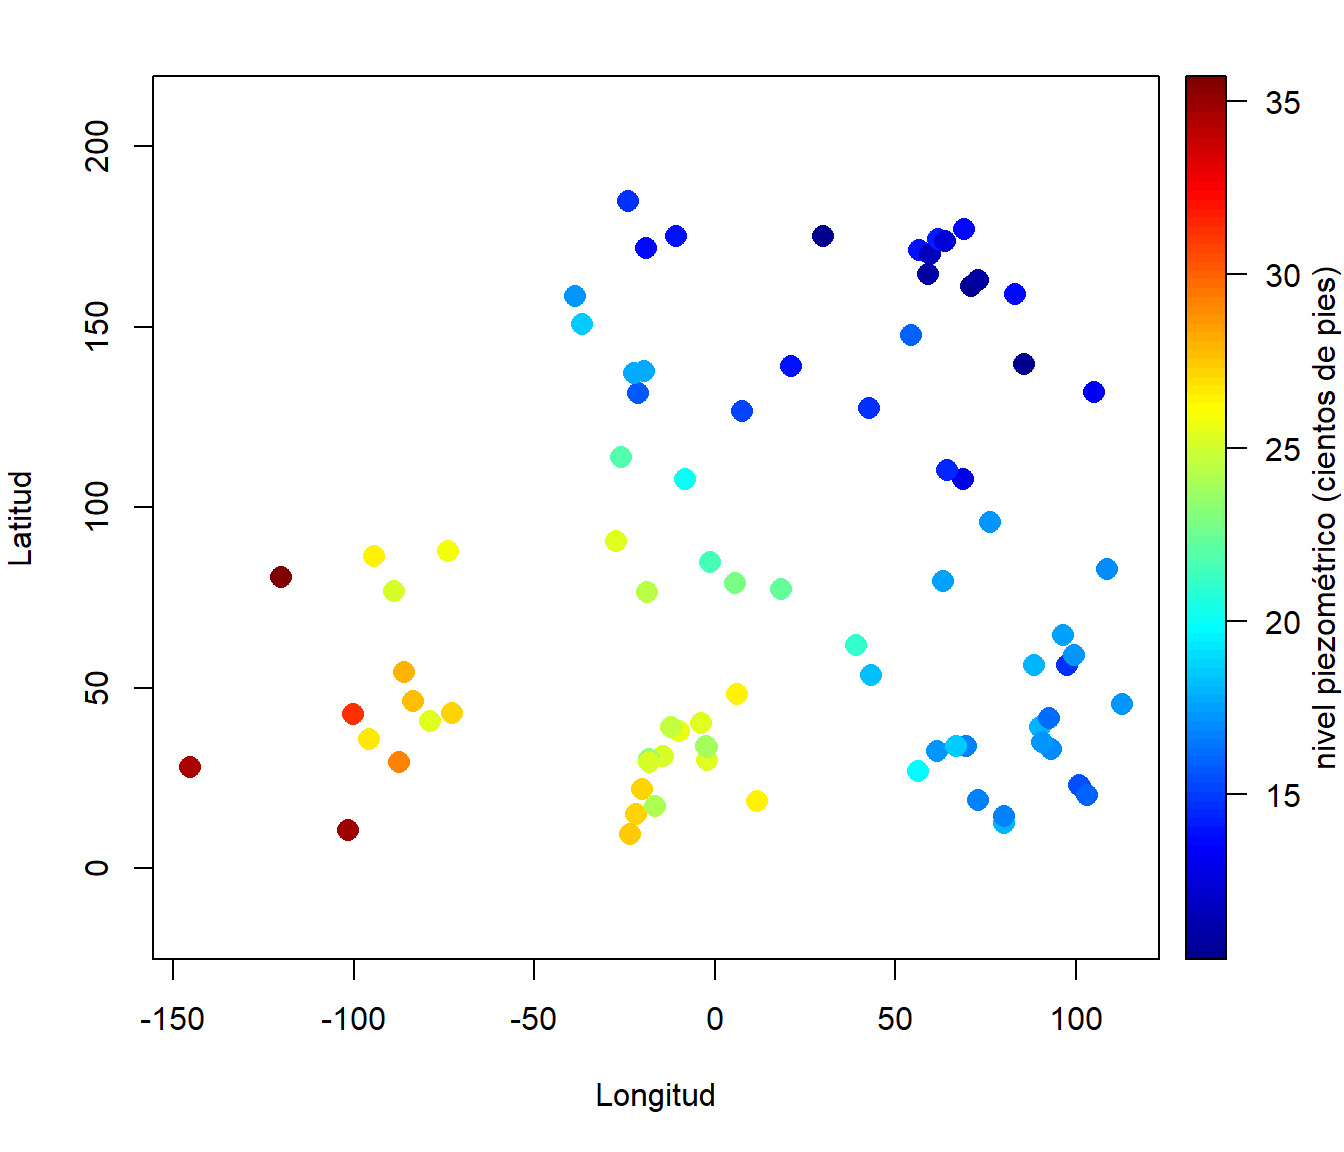
\includegraphics[width=0.7\linewidth]{01-introduccion_files/figure-latex/aquifer-1} 

  }

  \caption{Nivel del agua subterránea en 85 localizaciones del acuífero Wolfcamp (procedentes de un estudio sobre el posible emplazamiento de un depósito de residuos nucleares).}\label{fig:aquifer}
  \end{figure}
\item
  \textbf{Procesos reticulares/regionales} (índice espacial discreto):
  \(D\) es un conjunto numerable de posiciones o regiones. El proceso solo puede ser
  observado en determinadas posiciones. Es habitual que los datos se correspondan
  con agregaciones (totales o valores medios) de una determinada zona (por ejemplo,
  países, provincias, ayuntamientos, zonas sanitarias\ldots). Son muy comunes en
  econometría o epidemiología. {[}Figura \ref{fig:mortalidad}{]}

  \begin{figure}[!htb]

  {\centering 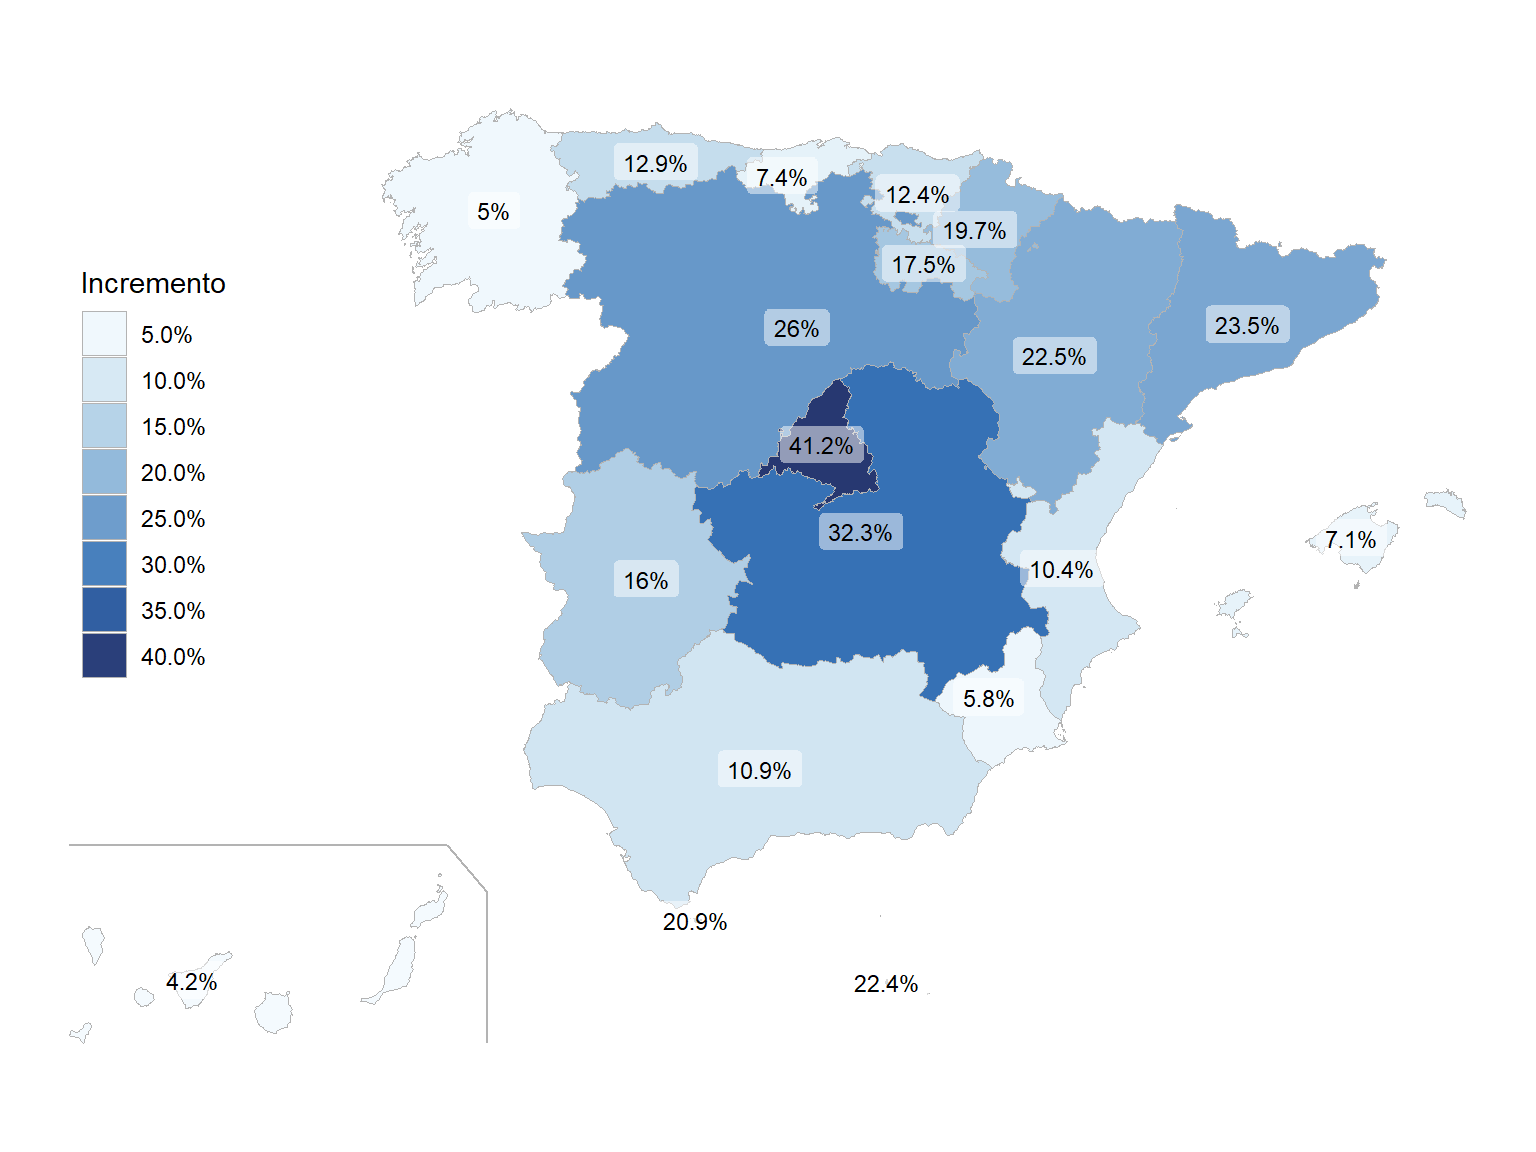
\includegraphics[width=0.7\linewidth]{01-introduccion_files/figure-latex/mortalidad-1} 

  }

  \caption{Porcentaje de incremento de las defunciones en el año 2020 respecto al 2019 por CCAA (datos provisionales [INE](https://www.ine.es/jaxi/Tabla.htm?tpx=21856)).}\label{fig:mortalidad}
  \end{figure}
\item
  \textbf{Procesos/patrones puntuales} (índice espacial aleatorio):
  \(D\) es un proceso puntual en \(\mathbb{R}^{d}\). Las posiciones en las que se
  observa el proceso son aleatorias. En muchas casos interesa únicamente la posición
  donde se observa el evento de interés (por ejemplo la posición en la que creció
  un árbol de una determinada especie). En el caso general, además de la posición
  se podría observar alguna otra característica (una marca; por ejemplo la altura o
  el diámetro del árbol), es lo que se conoce como \emph{proceso puntual marcado}.
  Este tipo de datos son habituales en biología, ecología, criminología, etc.
  {[}Figura \ref{fig:cholera}{]}

  \begin{figure}[!htb]

  {\centering 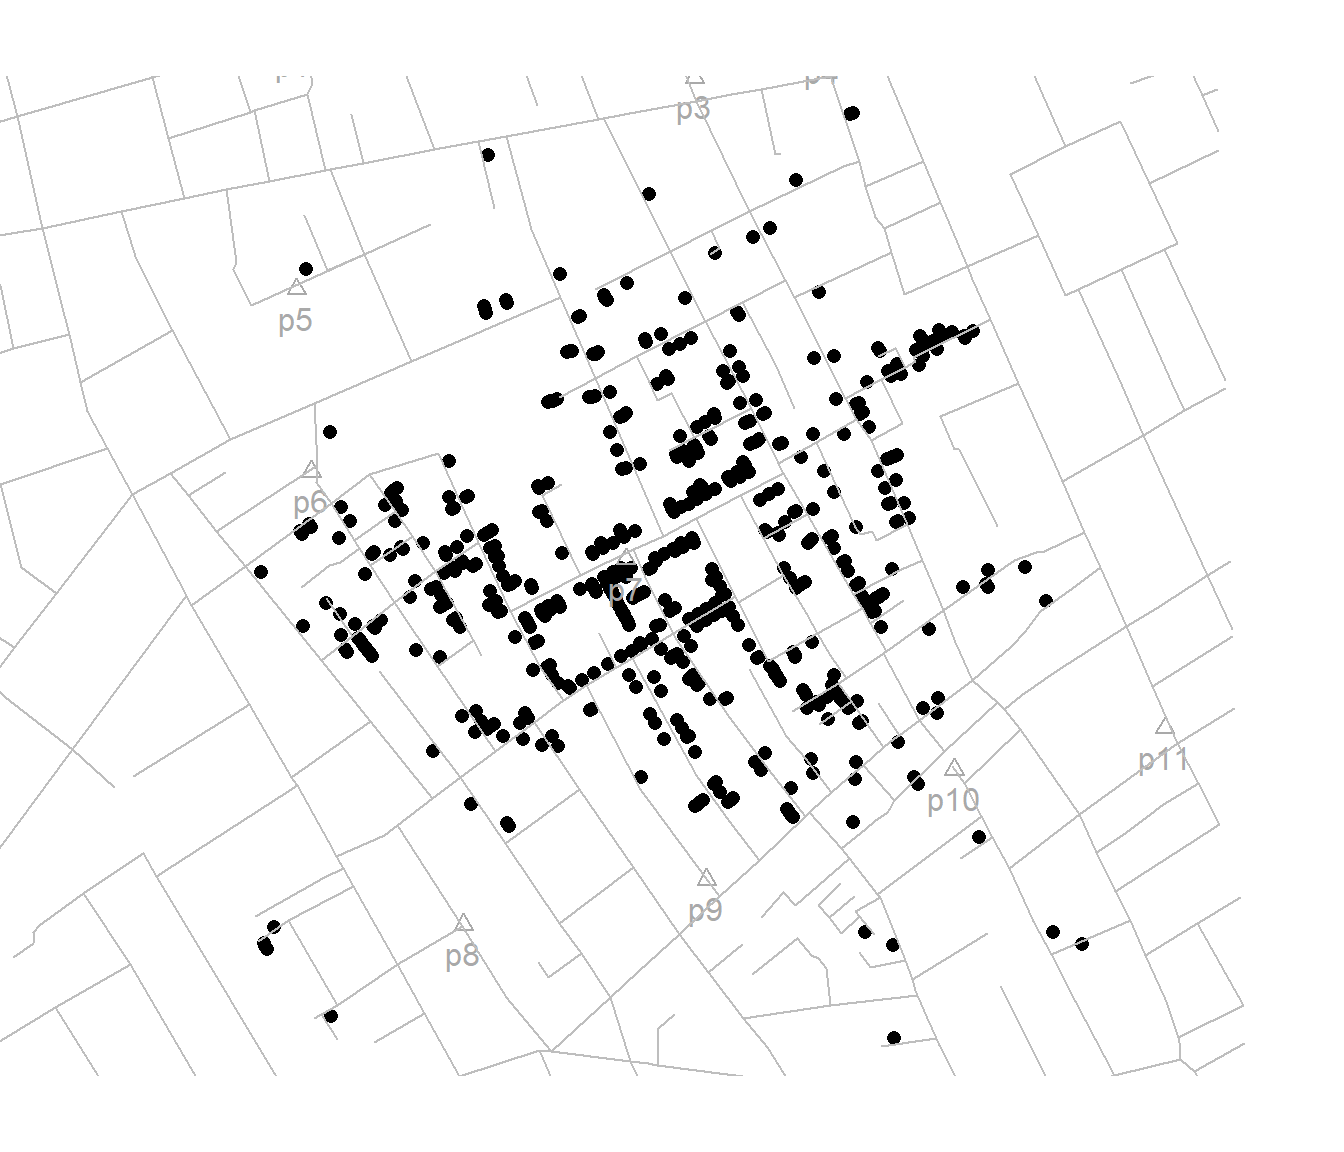
\includegraphics[width=0.7\linewidth]{01-introduccion_files/figure-latex/cholera-1} 

  }

  \caption{Mapa (de John Snow) del brote de cólera de 1854 en Londres.}\label{fig:cholera}
  \end{figure}
\end{itemize}

Nos centraremos en el caso de procesos geoestadísticos (también denominados procesos espaciales continuos).
El caso de posiciones espaciales discretas se considerará como resultado de la discretización de un proceso continuo.
Esto sería válido también para el caso espacio-temporal, por ejemplo podríamos considerar posiciones de la forma \(\mathbf{s}=(s_{1} , \ldots,s_{d-1} ,t) \in \mathbb{R}^{d-1} \times \mathbb{R}^{+,0}\), donde \(\mathbb{R}^{+,0} = \left\{ t \in \mathbb{R} : t \geq 0 \right\}\).
Por tanto, las definiciones y métodos para procesos espaciales son en principio aplicables también al caso espacio-temporal.
Sin embargo, la componente temporal presenta diferencias respecto a la componente espacial\ldots{}

\hypertarget{paquetes-r}{%
\subsection{Paquetes de R}\label{paquetes-r}}

En R hay disponibles una gran cantidad de paquetes para el análisis estadístico de datos espaciales (ver por ejemplo \href{http://cran.r-project.org/web/views/Spatial.html}{CRAN Task View: Analysis of Spatial Data}).
Entre ellos podríamos destacar:

\begin{itemize}
\item
  Procesos geoestadísticos: \texttt{gstat}, \texttt{geoR}, \texttt{geoRglm}, \texttt{fields},
  \texttt{spBayes}, \texttt{RandomFields}, \texttt{VR:spatial}, \texttt{sgeostat}, \texttt{vardiag}, \texttt{npsp}\ldots{}
\item
  Procesos reticulares/regionales: \texttt{spdep}, \texttt{DCluster}, \texttt{spgwr},
  \texttt{ade4}\ldots{}
\item
  Procesos puntuales: \texttt{spatstat}, \texttt{VR:spatial}, \texttt{splancs}\ldots{}
\end{itemize}

Algunos de estos paquetes son la referencia para el análisis de este tipo de datos,
aunque también están disponibles otros, como por ejemplo \texttt{maptools}, \texttt{geosphere}, \texttt{tmap}, \texttt{mapsf}, \texttt{leaflet}, \texttt{mapview}, \texttt{mapdeck}, \texttt{ggmap}, \texttt{rgrass7}, \texttt{RSAGA}, \texttt{RPyGeo}, \texttt{RQGIS} o \texttt{r-arcgis}, que implementan herramientas adicionales y permiten, por ejemplo, generar gráficos interactivos o interactuar con sistemas externos de información geográfica (GIS).

En todos estos paquetes se trabajan con similares tipos de datos (espaciales y espacio-temporales) por lo que se han desarrollado paquetes que facilitan su manejo.
Entre ellos destacan el paquete \href{https://CRAN.R-project.org/package=sp}{\texttt{sp}} \protect\hyperlink{ref-Bivand2013}{Bivand et~al.} (\protect\hyperlink{ref-Bivand2013}{2013}) y el paquete \href{https://r-spatial.github.io/sf}{\texttt{sf}} \protect\hyperlink{ref-Pebesma2021}{E. Pebesma y Bivand} (\protect\hyperlink{ref-Pebesma2021}{2021}).
Otros paquetes para la manipulación de datos que pueden ser de interés son: \href{https://CRAN.R-project.org/package=raster}{\texttt{raster}}, \href{https://CRAN.R-project.org/package=terra}{\texttt{terra}}, \href{https://r-spatial.github.io/stars}{\texttt{starts}}, \href{https://CRAN.R-project.org/package=rgdal}{\texttt{rgdal}} y \href{https://CRAN.R-project.org/package=rgeos}{\texttt{rgeos}}, entre otros.
En la Sección \ref{datos-tipos} se incluye información adicional sobre estos paquetes.

En estos apuntes emplearemos principalmente el paquete \texttt{gstat} para el análisis de datos geoestadísticos (aunque se incluye una introducción al paquete \texttt{geoR} en el Apéndice B) y el paquete \texttt{sf} para la manipulación de datos espaciales (en el Apéndice A se incluye una breve introducción a las clases \texttt{sp} para datos espaciales).

\hypertarget{geoestadistica}{%
\section{Geoestadística}\label{geoestadistica}}

La geoestadística (Matheron 1962) surgió como una mezcla de varias disciplinas: ingeniería de minas, geología, matemáticas y estadística, para dar respuesta a problemas como, por ejemplo, el de la estimación de los recursos de una explotación minera (se desarrolló principalmente a partir de los años 80).
La diferencia (ventaja) respecto a otras aproximaciones es que, además de tener en cuenta la tendencia espacial (variación de gran escala), también tiene en cuenta la correlación espacial (variación de pequeña escala).
Otros métodos sin embargo, sólo incluyen la variación de larga escala y suponen que los errores son independientes (Sección \ref{modelos-clasicos-espaciales}).
Hoy en día podemos decir que la geoestadística es la rama de la estadística espacial que estudia los procesos con índice espacial continuo.

Uno de los problemas iniciales más importantes de la geoestadística fue la predicción de la riqueza de un bloque minero a partir de una muestra observada.
A este proceso Matheron (1963) lo denominó kriging\footnote{D. G. Krige fue un ingeniero de minas de Sudáfrica que desarrollo
  en los años 50 métodos empíricos para determinar la distribución de
  la riqueza de un mineral a partir de valores observados.
  Sin embargo la formulación de la predicción espacial lineal óptima no
  procede del trabajo de Krige.
  Al mismo tiempo que la geoestadística se desarrollaba en la ingeniería
  de minas por Matheron en Francia, la misma idea se desarrollaba en la
  meteorología por L.S. Gandin en la antigua Unión Soviética.
  El nombre que Gandin le dio a esta aproximación fue análisis objetivo
  y utilizó la terminología de interpolación óptima en lugar de kriging.
  Para más detalles sobre el origen del kriging ver p.e. Cressie (1990).}, y también predicción espacial lineal óptima (estos métodos de predicción se muestran en el Capítulo 4).

El modelo general habitualmente considerado en geoestadística considera que el proceso se descompone en \emph{variabilidad de gran escala} y \emph{variabilidad de pequeña escala}:
\begin{equation}
  Z(\mathbf{s}) = \mu(\mathbf{s}) + \varepsilon(\mathbf{s}),
  \label{eq:modelogeneral}
\end{equation}
donde:

\begin{itemize}
\item
  \(\mu(\mathbf{s}) = E \left( Z(\mathbf{s}) \right)\) es la tendencia (función de regresión, determinística).
\item
  \(\varepsilon(\mathbf{s})\) es un proceso de error de media cero que incorpora la dependencia espacial.
\end{itemize}

Como en condiciones normales únicamente se dispone de una realización parcial del proceso, se suelen asumir hipótesis adicionales de estacionariedad sobre el proceso de error \(\varepsilon(\mathbf{s})\) para hacer posible la inferencia.
En la Sección \ref{procesos-estacionarios} se definen los principales tipos de estacionariedad habitualmente considerados en geoestadística y se introducen dos funciones relacionadas con procesos estacionarios, el covariograma y el variograma.
Algunas propiedades de estas funciones, que podríamos decir que son las herramientas fundamentales de la geoestadística, se muestran en la Sección 2.2.

\hypertarget{modelos-clasicos-espaciales}{%
\subsection{Modelos clásicos y modelos espaciales}\label{modelos-clasicos-espaciales}}

En general, cuando se considera que la componente espacial (o espacio-temporal) puede ser importante en el modelado y el análisis de los datos es necesaria una aproximación estadística distinta a la tradicionalmente usada.

Uno de los modelos más utilizados en estadística para el caso de datos no homogéneos es el conocido modelo clásico de regresión lineal.
Si \(\left\{ Z(\mathbf{s}):\mathbf{s}\in D\subset \mathbb{R}^{d} \right\}\) es un proceso espacial, podemos suponer que:
\[Z(\mathbf{s})=\sum\limits_{j=0}^{p}x_{j}(\mathbf{s})\beta_{j} +\varepsilon(\mathbf{s}),\ \mathbf{s}\in D,\]
(un caso particular del modelo general \eqref{eq:modelogeneral}), donde \(\boldsymbol{\beta }=(\beta_{0}, \ldots,\beta_{p})^{\top}\in \mathbb{R}^{p+1}\) es un vector desconocido, \(\left\{ x_{j} (\cdot):j=0, \ldots,p\right\}\) un conjunto de variables explicativas (típicamente \(x_0(\cdot)=1\)) y \(\varepsilon(\cdot)\) un proceso de media cero incorrelado (i.e.~\(Cov(\varepsilon (\mathbf{u}),\varepsilon (\mathbf{v}))=0\) si \(\mathbf{u}\neq \mathbf{v}\)) con \(Var(\varepsilon (\mathbf{s}))=\sigma^{2}\).

Supongamos por el momento que el objetivo es la estimación eficiente de la tendencia, o lo que es lo mismo la estimación óptima de los parámetros de la \emph{variación de gran escala} \(\boldsymbol{\beta}\), a partir de los datos observados en un conjunto de posiciones espaciales \(\left\{ \mathbf{s}_{1}, \ldots,\mathbf{s}_{n} \right\}\).
Bajo las hipótesis anteriores:
\[\mathbf{Z} = \mathbf{X}\boldsymbol{\beta} + \boldsymbol{\varepsilon},\]
siendo \(\mathbf{Z}=\left( Z(\mathbf{s}_{1}), \ldots,Z(\mathbf{s}_{n}) \right)^{\top}\), \(\mathbf{X}\) una matriz \(n\times (p+1)\) con \(X_{ij}=x_{j-1}(\mathbf{s}_{i})\) y \(\boldsymbol{\varepsilon} = \left( \varepsilon (\mathbf{s}_{1}), \ldots,\varepsilon (\mathbf{s}_{n})\right)^{\top}\); y el estimador lineal insesgado de \(\boldsymbol{\beta}\) más eficiente resulta ser el estimador de mínimos cuadrados ordinarios (OLS, \emph{ordinary least squares}):
\begin{equation} 
  \hat{\boldsymbol{\beta}}_{ols}=(\mathbf{X}^{\top}\mathbf{X})^{-1}\mathbf{X}^{\top}\mathbf{Z},
  \label{eq:beta-ols}
\end{equation}
con \[Var(\hat{\boldsymbol{\beta}}_{ols})=\sigma^{2}(\mathbf{X}^{\top}\mathbf{X})^{-1}.\]

Sin embargo la suposición de que los errores son independientes e idénticamente distribuidos influye crucialmente en la inferencia.
En el modelo anterior, en lugar de errores incorrelados, si suponemos que:
\[Var\left( \boldsymbol{\varepsilon} \right) =\Sigma,\]
obtenemos el modelo lineal de regresión generalizado y en este caso el estimador lineal óptimo de \(\boldsymbol{\beta}\) es el estimador de mínimos cuadrados generalizados (GLS, \emph{generalized least squares}):
\begin{equation} 
  \hat{\boldsymbol{\beta}}_{gls} =(\mathbf{X}^{\top}\Sigma^{-1} \mathbf{X})^{-1} \mathbf{X}^{\top}\Sigma^{-1} \mathbf{Z}.
  \label{eq:beta-gls}
\end{equation}

Si \(\Sigma=\sigma^{2} \mathbf{I}_{n}\), siendo \(\mathbf{I}_{n}\) la matriz identidad \(n\times n\), los estimadores \eqref{eq:beta-ols} y \eqref{eq:beta-gls} coinciden; pero en caso contrario las estimaciones basadas en el modelo anterior pueden llegar a ser altamente ineficientes.
Puede verse fácilmente que en el caso general:
\[Var\left( \hat{\boldsymbol{\beta}}_{gls} \right)=(\mathbf{X}^{\top}\Sigma^{-1} \mathbf{X})^{-1}, \\
Var\left( \hat{\boldsymbol{\beta}}_{ols} \right) =(\mathbf{X}^{\top}\mathbf{X})^{-1} (\mathbf{X}^{\top}\Sigma\mathbf{X})(\mathbf{X}^{\top}\mathbf{X})^{-1},\]
resultando además que \(Var( \hat{\boldsymbol{\beta}}_{ols}) - Var( \hat{\boldsymbol{\beta}}_{gls} )\) es una matriz semidefinida positiva (e.g.~Searle, 1971, Sección 3.3).

En muchos casos el objetivo final es la predicción del proceso en una posición espacial \(\mathbf{s}_{0}\):
\[Z(\mathbf{s}_{0} )=\mathbf{x}^{\top}\boldsymbol{\beta}+\varepsilon (\mathbf{s}_{0} ),\]
donde \(\mathbf{x}=\left( x_{0} (\mathbf{s}_{0} ), \ldots,x_{p} (\mathbf{s}_{0})\right)^{\top}\).
Bajo las hipótesis del modelo clásico el predictor óptimo sería la estimación de la tendencia \(\hat{\mu}(\mathbf{s}_{0} ) = \mathbf{x}^{\top}\hat{\boldsymbol{\beta}}_{ols}\) (el predictor óptimo de un error independiente sería cero).
En el caso general, siguiendo esta aproximación, podríamos pensar en utilizar como predictor el estimador más eficiente de la tendencia:
\[\hat{Z} (\mathbf{s}_{0})=\mathbf{x^{\top}}\hat{\boldsymbol{\beta}}_{gls},\]
sin embargo no es el predictor lineal óptimo. Puede verse (e.g.~Goldberger, 1962; Sección 4.X) que en este caso el mejor predictor lineal insesgado es:
\begin{equation} 
  \tilde{Z}(\mathbf{s}_{0}) = \mathbf{x}^{\top}\hat{\boldsymbol{\beta}}_{gls} + \mathbf{c}^{\top} \Sigma^{-1} \left( \mathbf{Z} - \mathbf{X}\hat{\boldsymbol{\beta}}_{gls} \right),
  \label{eq:predictor-kriging}
\end{equation}
(el denominado predictor del \emph{kriging universal}, Sección 4.X), siendo
\[\mathbf{c} = \left( Cov\left( \varepsilon (\mathbf{s}_{1} ),\varepsilon (\mathbf{s}_{0} )\right), \ldots, Cov\left( \varepsilon (\mathbf{s}_{n} ),\varepsilon (\mathbf{s}_{0} )\right) \right)^{\top},\]
y la diferencia \(Var( \hat{Z} (\mathbf{s}_{0} ) ) - Var( \tilde{Z} (\mathbf{s}_{0} ) ) \ge 0\) puede ser significativamente mayor que cero\footnote{Por ejemplo, para un caso particular, Goldberger (1962, pp.374-375) observó que la mejora en la predicción puede llegar a ser del 50\%. En Cressie (1993, Sección 1.3) se muestran también otros ejemplos del efecto de la presencia de correlación en la estimación.} (si la dependencia espacial no es muy débil).
Naturalmente, si se ignora por completo la dependencia y se emplea únicamente el estimador \(\hat{\boldsymbol{\beta}}_{ols}\) disminuye aún más la eficiencia de las predicciones.

Teniendo en cuenta los resultados anteriores podemos afirmar que al explotar la dependencia presente en los datos el incremento en eficiencia puede ser importante.
Sin embargo el principal inconveniente es que en la práctica normalmente la matriz \(\Sigma\) y el vector \(\mathbf{c}\) son desconocidos.
El procedimiento habitual, para evitar la estimación de \(n+n(n+1)/2\) parámetros adicionales a partir del
conjunto de \(n\) observaciones, suele ser la elección de un modelo paramétrico adecuado:
\[C(\mathbf{u},\mathbf{v}\left| \boldsymbol{\theta}\right. )\equiv Cov\left( \varepsilon (\mathbf{u}),\varepsilon (\mathbf{v})\right),\]
i.e.~suponer que \(\Sigma \equiv \Sigma\left( \boldsymbol{\theta}\right)\) y \(\mathbf{c}\equiv \mathbf{c}\left( \boldsymbol{\theta}\right)\).
Una hipótesis natural es suponer que los datos cercanos en el espacio o en el tiempo están correlados y que la correlación disminuye al aumentar la separación entre ellos; por tanto es normal pensar en errores espacialmente correlados.
Por ejemplo, podemos considerar:
\[C(\mathbf{u},\mathbf{v}\left| \boldsymbol{\theta}\right. )=\sigma^{2} \rho^{\left\| \mathbf{u}-\mathbf{v}\right\| },\]
con \(\sigma^{2} \geq 0\) y \(0<\rho <1\).
De esta forma, si \(\hat{\boldsymbol{\theta}}\) es un estimador de \(\boldsymbol{\theta}\), podemos obtener por ejemplo una aproximación del predictor óptimo de \(Z(\mathbf{s}_{0} )\) sustituyendo en \eqref{eq:predictor-kriging} \(\Sigma(\boldsymbol{\theta})\) por \(\Sigma(\hat{\boldsymbol{\theta}} )\) y \(\mathbf{c}(\boldsymbol{\theta})\) por \(\mathbf{c}(\hat{\boldsymbol{\theta}} )\).

\hypertarget{ventajas-de-la-aproximaciuxf3n-espacial-y-espacio-temporal}{%
\subsection{Ventajas de la aproximación espacial (y espacio-temporal)}\label{ventajas-de-la-aproximaciuxf3n-espacial-y-espacio-temporal}}

Algunos de los beneficios de utilizar modelos espaciales para caracterizar y explotar la dependencia espacial de un conjunto de datos son los siguientes:

\begin{itemize}
\item
  Modelos más generales: en la mayoría de los casos, los modelos clásicos no espaciales son un caso particular de un modelo espacial.
\item
  Estimaciones más eficientes: de la tendencia, de los efectos de variables explicativas, de promedios regionales\ldots{}
\item
  Mejora de las predicciones: más eficientes, con propiedades de extrapolación más estables\ldots{}
\item
  La variación espacial no explicada en la estructura de la media debe ser absorbida por la estructura del error, por lo que un modelo que incorpore la dependencia espacial puede decirse que esta protegido frente a una mala especificación de este tipo. Esto en muchos casos tiene como resultado una simplificación en la especificación de la tendencia; en general los modelos con dependencia espacial suelen tener una descripción más parsimoniosa (en ocasiones con muchos menos parámetros) que los clásicos modelos de superficie de tendencia.
\end{itemize}

\hypertarget{procesos-estacionarios}{%
\section{Procesos espaciales estacionarios}\label{procesos-estacionarios}}

Supongamos que \(\left\{ Z(\mathbf{s}) : \mathbf{s} \in D \subset \mathbb{R}^{d} \right\}\) es un proceso geoestadístico.
Este proceso aleatorio se puede caracterizar a través de las funciones de distribución finito-dimensionales:
\[F_{\mathbf{s}_1, \ldots, \mathbf{s}_m}(z_1, \ldots, z_m)
= P\left(Z(\mathbf{s}_1)\leq z_1 , \ldots,Z(\mathbf{s}_m)\leq z_m \right)\]
(o de las funciones de densidad correspondientes \(f_{\mathbf{s}_1, \ldots, \mathbf{s}_m}(z_1, \ldots, z_m)\).
Por ejemplo, el proceso se dice normal (o gaussiano) si para cada posible conjunto de \(m \in \mathbb{N}\) posiciones espaciales, \(\{\mathbf{s}_1, \ldots, \mathbf{s}_m\}\), su función de distribución \(F_{\mathbf{s}_1, \ldots, \mathbf{s}_m}\) es normal (gaussiana).

Como ya se comentó en la Sección \ref{proc-esp}, en general no se puede disponer de una realización completa del proceso \(Z(\cdot)\) y solamente se observan valores en unas posiciones espaciales conocidas \(\left\{ \mathbf{s}_1, \ldots, \mathbf{s}_{n} \right\}\) (que por lo general van a ser irregulares).
Por tanto es necesario hacer algunas suposiciones acerca del proceso de forma que sea posible la inferencia sobre el mismo.
Lo habitual es asumir algún tipo de estacionariedad del proceso (o del proceso de error, suponiendo que el proceso no tiene media constante y sigue el modelo general \eqref{eq:modelogeneral}).

El proceso \(Z(\cdot)\) se dice \emph{estrictamente estacionario} si al trasladar (en cualquier dirección) una configuración cualquiera de posiciones espaciales la distribución conjunta no varia:
\[F_{\mathbf{s}_1 +\mathbf{h}, \ldots,\mathbf{s}_m +\mathbf{h}}(z_1, \ldots, z_m) = F_{\mathbf{s}_1, \ldots, \mathbf{s}_m}(z_1, \ldots, z_m),\ \forall \mathbf{h}\in D,\ \forall m\geq 1.\]

El proceso \(Z(\cdot)\) se dice \emph{estacionario de segundo orden} (también proceso estacionario homogéneo o débilmente estacionario) si tiene media constante y la covarianza entre dos posiciones depende únicamente del salto entre ellas:

\begin{itemize}
\item
  \(E(Z(\mathbf{s}))=\mu,\ \forall \mathbf{s}\in D\).
\item
  \(Cov(Z(\mathbf{s}_1), Z(\mathbf{s}_2)) = C(\mathbf{s}_1 -\mathbf{s}_2),\ \forall \mathbf{s}_1 ,\mathbf{s}_2 \in D\).
\end{itemize}

La función \(C(\cdot)\) se denomina \emph{covariograma} (también autocovariograma o función de covarianzas).
Si además \(C(\mathbf{h}) \equiv C(\left\| \mathbf{h}\right\|)\) (sólo depende de la magnitud y no de la dirección del salto) se dice que el covariograma es \emph{isotrópico} (en caso contrario se dice que es \emph{anisotrópico}; \ref{anisotropia}).

Si un proceso es estrictamente estacionario y \(Var(Z(\mathbf{s}))\) es finita, entonces es estacionario de segundo orden.
Además, como es bien conocido, en el caso de procesos normales ambas propiedades son equivalentes (ya que están caracterizados por su media y covarianza).

En algunos casos en lugar del covariograma se utiliza el correlograma:
\[\rho (\mathbf{h}) = \dfrac{C(\mathbf{h})}{C(\mathbf{0})} \in \left[-1,+1\right],\]
suponiendo que \(C(\mathbf{0}) = Var(Z(\mathbf{s})) >0\).
Sin embargo lo habitual es modelar la dependencia espacial a través del variograma (principalmente por sus ventajas en la estimación; Sección \ref{vario-muestrales}), definido a continuación.

Se dice que el proceso es \emph{intrínsecamente estacionario} (también proceso espacial de incrementos estacionarios u homogéneos) si:

\begin{itemize}
\item
  \(E(Z(\mathbf{s}))=\mu,\ \forall \mathbf{s}\in D\).
\item
  \(Var(Z(\mathbf{s}_1)-Z(\mathbf{s}_2)) = 2\gamma (\mathbf{s}_1 - \mathbf{s}_2),\ \forall \mathbf{s}_1 ,\mathbf{s}_2 \in D\).
\end{itemize}

La función \(2\gamma (\cdot)\) se denomina \emph{variograma} y \(\gamma (\cdot)\) \emph{semivariograma}.
Al igual que en el caso anterior, si además \(\gamma(\mathbf{h}) \equiv \gamma(\left\| \mathbf{h}\right\|)\) (sólo depende de la distancia) se dice que el variograma es isotrópico.

La clase de procesos intrínsecamente estacionarios es más general que la clase de procesos estacionarios de segundo orden.
Si un proceso estacionario de segundo orden tiene covariograma \(C(\cdot)\), como:
\[\begin{aligned}
Var(Z(\mathbf{s}_1)-Z(\mathbf{s}_2)) &= Var(Z(\mathbf{s}_1)) + Var(Z(\mathbf{s}_2))-2Cov(Z(\mathbf{s}_1),Z(\mathbf{s}_2)) \\
&=2\left(C(\mathbf{0})-C(\mathbf{s}_1 -\mathbf{s}_2)\right),
\end{aligned}\]
entonces su semivariograma viene dado por:
\[\gamma (\mathbf{h}) = C(\mathbf{0})-C(\mathbf{h}),\]
y por tanto es un proceso intrínsecamente estacionario.
El reciproco en general no es cierto (por ejemplo el caso de un \href{https://es.wikipedia.org/wiki/Movimiento_browniano\#Matem\%C3\%A1ticas}{movimiento browniano}), aunque sí se verifica en muchos casos.
Normalmente cuando no se verifica es debido a que el proceso no tiene media constante y puede ser modelado como una función de tendencia más un error estacionario de segundo orden (o cuando se consideran los errores del modelo general, la tendencia no está especificada correctamente).

Si el variograma está acotado y:
\[\lim \limits_{\left\| \mathbf{h}\right\| \rightarrow \infty }\gamma(\mathbf{h})=\sigma^2,\]
entonces\footnote{Suponiendo que \(\lim \limits_{\left\| \mathbf{h}\right\| \rightarrow \infty } C(\mathbf{h})=0\).} podemos obtener el covariograma correspondiente como:
\[C(\mathbf{h})=\sigma^2-\gamma (\mathbf{h}).\]
A \(\sigma^{2} = C(\mathbf{0})\) se le denomina \emph{umbral} (o \emph{meseta}) del semivariograma.
La relación entre el semivariograma y el covariograma se ilustra en la Figura \ref{fig:var-gen}.

Además del umbral, hay otras características geométricas del variograma (o del covariograma) de especial importancia\footnote{Además de poder interpretar su influencia en la predicción espacial (Sección 4.X), son utilizadas en la parametrización de la mayoría de los modelos de variogramas o covariogramas (Sección \ref{modelos-parametricos}).}, entre ellas destacarían el \emph{efecto pepita} (o \emph{nugget}) y el \emph{rango} (o \emph{alcance}).
La Figura \ref{fig:var-gen} ilustra las distintas características del semivariograma.

\begin{figure}[!htb]

{\centering 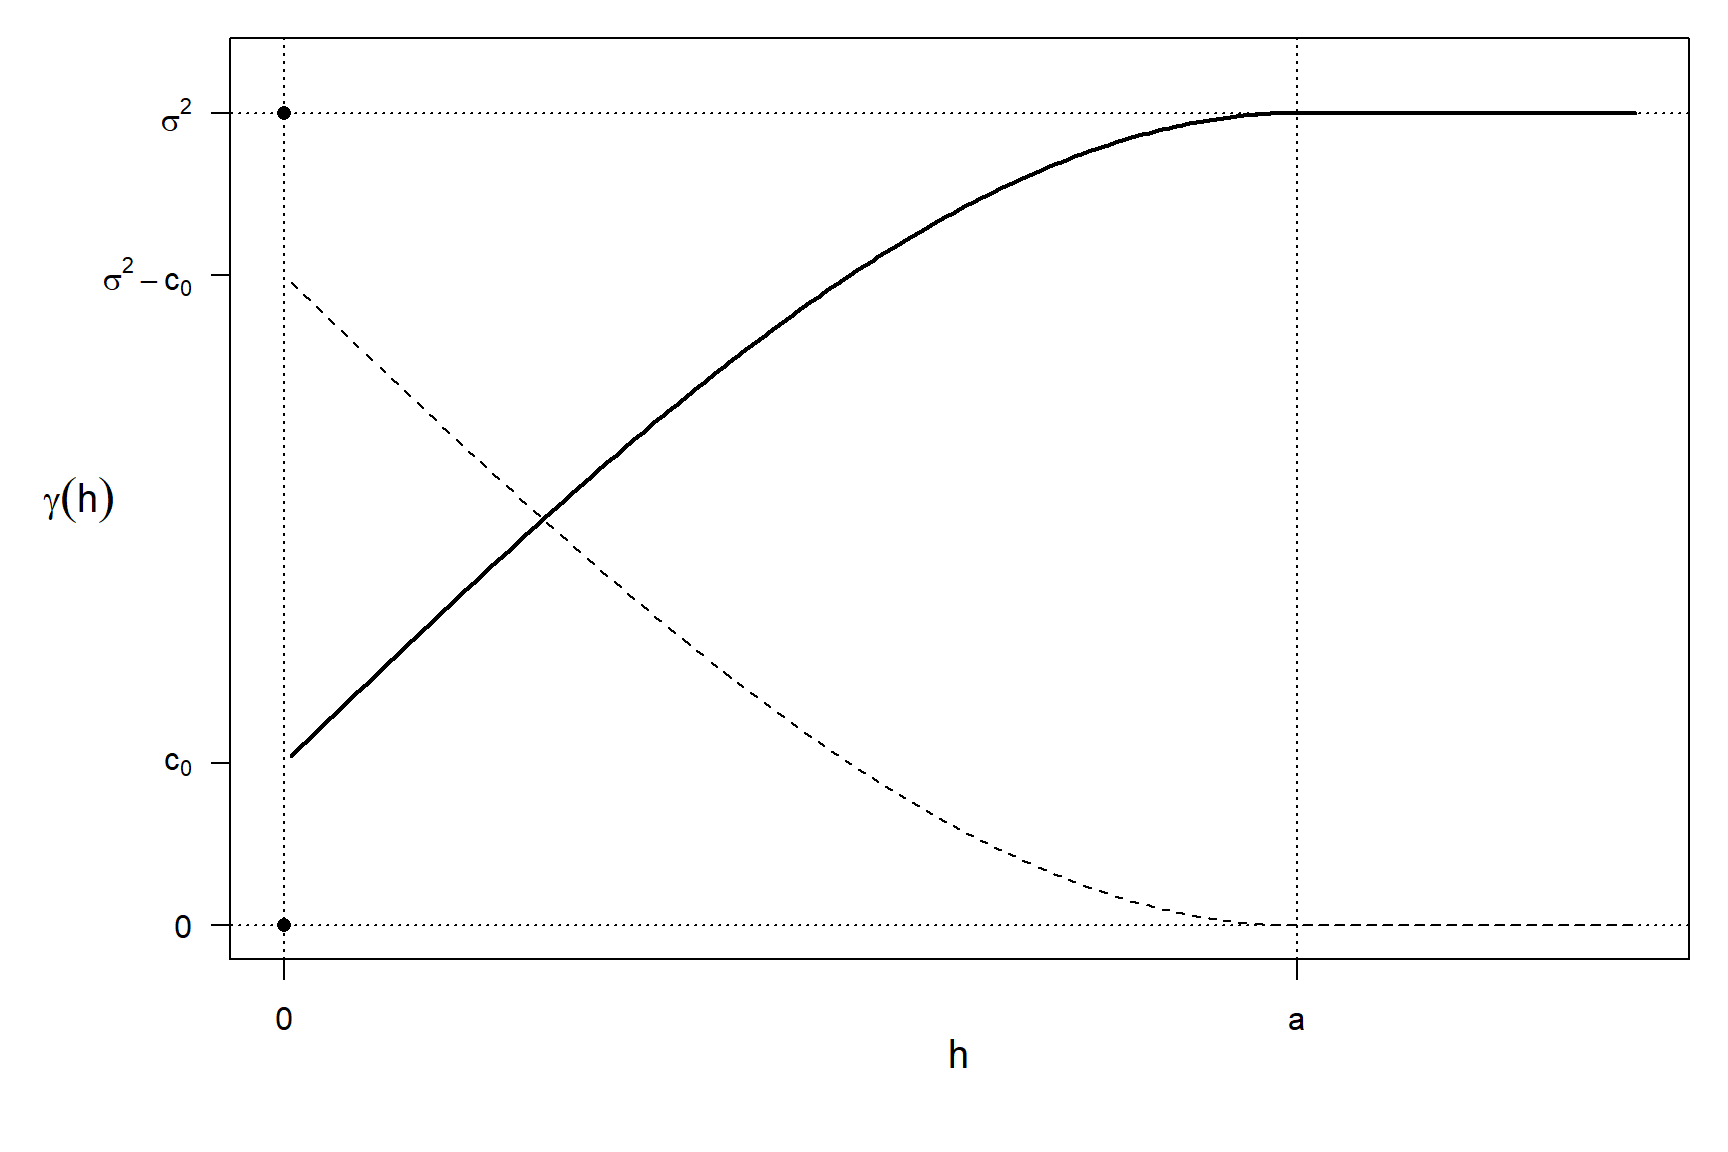
\includegraphics[width=0.8\linewidth]{01-introduccion_files/figure-latex/var-gen-1} 

}

\caption{Relación entre el covariograma (línea discontinua) y el variograma (línea continua) en el caso unidimensional (o isotrópico), y principales características.}\label{fig:var-gen}
\end{figure}

Siempre se verifica que \(\gamma (\mathbf{0})=0\), sin embargo puede ser que:
\[\lim \limits_{\mathbf{h}\rightarrow \mathbf{0}} \gamma(\mathbf{h}) = c_0 > 0.\]
entonces \(c_0\) se denomina \emph{efecto pepita} (o \emph{nugget})\footnote{El origen de esta denominación esta relacionado con la terminología minera. En algunos yacimientos de metal, como por ejemplo en el caso del oro, el mineral suele obtenerse como pepitas de material puro y estas pepitas normalmente son más pequeñas que el tamaño de la unidad de muestreo (lo que produce una variabilidad adicional en la muestra).}.
Además, si \(\sigma^{2}\) es el umbral del semivariograma (suponiendo que existe), a \(\sigma ^{2} -c_0\) se le denomina \emph{umbral parcial}.

Las propiedades de continuidad (y derivabilidad) del variograma (o el covariograma) en el origen están relacionadas con las propiedades de continuidad (y diferenciabilidad) en media cuadrática del proceso \(Z(\cdot)\) (ver e.g.~Chilès y Delfiner, 1999, Sección 2.3.1).
Por ejemplo, el proceso es continuo en media cuadrática si y sólo si su variograma (covariograma) es continuo en el origen. Entonces la presencia de efecto nugget indica que (en teoría) el proceso no es continuo y por tanto altamente irregular.

La proporción del efecto nugget en el umbral total \(c_0 /\sigma^{2}\) proporciona mucha información acerca del grado de dependencia espacial presente en los datos.
Por ejemplo, en el caso en que toda la variabilidad es efecto nugget (i.e.~\(\gamma (\mathbf{h})=c_0\), \(\forall \mathbf{h}\neq \mathbf{0}\)) entonces \(Z(\mathbf{s}_1)\) y \(Z(\mathbf{s}_2)\) son incorrelados \(\forall \mathbf{s}_1 ,\mathbf{s}_2 \in D\) independientemente de lo cerca que estén (el proceso \(Z(\cdot)\) es ruido blanco).
Por tanto podemos pensar en \(c_0 /\sigma^{2}\) como la proporción de ``variabilidad independiente'', aunque en la práctica típicamente no se dispone de información sobre el variograma a distancias menores de \(\min \left\{ \left\| \mathbf{s}_{i} -\mathbf{s}_{j} \right\| :1\leq i<j\leq n\right\}\) (la estimación de \(c_0\) se obtiene normalmente extrapolando un variograma experimental cerca del origen).

Si \(\sigma ^{2}\) es el umbral del semivariograma (suponiendo que existe), se define el \emph{rango} (o alcance) del semivariograma en la dirección \(\mathbf{e}_0 \in \mathbb{R}^{d}\) con \(\left\| \mathbf{e}_0 \right\| = 1\), como el mínimo salto en esa dirección en el que se alcanza el umbral:
\[a_0 =\min \left\{ a:\gamma (a\left( 1+\varepsilon \right) \mathbf{e}_0 )=\sigma ^{2} , \forall \varepsilon >0\right\}.\]
El rango en la dirección \(\mathbf{e}_0\) puede interpretarse como el salto \(h\) a partir del cual no hay correlación entre \(Z(\mathbf{s})\) y \(Z(\mathbf{s}\pm h\mathbf{e}_0)\), por tanto está íntimamente ligado a la noción de ``zona de influencia'' (y tiene un papel importante en la determinación de criterios de vecindad).
En los casos en los que el semivariograma alcanza el umbral asintóticamente (rango infinito), se suele considerar el \emph{rango práctico}, definido como el mínimo salto en el que se alcanza el 95\% del umbral.

El variograma y el covariograma son las funciones habitualmente consideradas en geoestadística para el modelado de la dependencia espacial (o espacio-temporal), y son consideradas como un parámetro (de especial interés) del proceso.
En la práctica normalmente se suele utilizar el variograma, no sólo porque es más general (puede existir en casos en que el covariograma no), sino por las ventajas en su estimación (Sección \ref{vario-muestrales}; Cressie, 1993, Sección 2.4.1).
No obstante, en muchos casos los modelos de variograma se obtienen a partir de modelos de covariograma.

\hypertarget{propiedades-elementales}{%
\subsection{Propiedades elementales del covariograma y del variograma}\label{propiedades-elementales}}

El variograma y el covariograma deben verificar ciertas propiedades que sus estimadores no siempre verifican, a continuación se detallan algunas de ellas.

Si \(Z(\cdot)\) es un proceso estacionario de segundo orden con covariograma \(C(\cdot)\),
entonces se verifica que \(C(\mathbf{0}) = Var( Z(\mathbf{s}) ) \geq 0\), es una función par \(C(\mathbf{h})=C(-\mathbf{h})\), y por la desigualdad de Cauchy-Schwarz \(\left| C(\mathbf{h})\right| \leq C(\mathbf{0})\).
Además, el covariograma debe ser semidefinido positivo, es decir:
\[\sum\limits_{i=1}^{m} \sum\limits_{j=1}^{m} a_i a_j C(\mathbf{s}_i-\mathbf{s}_j) \geq 0  \\
\forall m\geq 1,\ \forall \mathbf{s}_i \in D,\ \forall a_i \in \mathbb{R};\ i=1, \ldots,m,\]
ya que:
\[\sum\limits_{i=1}^{m}\sum\limits_{j=1}^{m}a_i a_j C(\mathbf{s}_i -\mathbf{s}_j) = Var\left\{\sum\limits_{i=1}^{m}a_i Z(\mathbf{s}_i) \right\}\]
La condición es necesaria y suficiente para que exista un proceso estacionario de segundo orden con covariograma \(C(\cdot)\) (se puede construir un proceso normal multivariante con covarianzas definidas por \(C(\cdot)\)).
Por tanto la clase de covariogramas válidos en \(\mathbb{R}^d\) es equivalente a la clase de funciones semidefinidas positivas en \(\mathbb{R}^d\).

Algunas propiedades adicionales que verifican los covariogramas son las siguientes:

\begin{enumerate}
\def\labelenumi{\arabic{enumi}.}
\item
  Si \(C(\cdot)\) es un covariograma válido en \(\mathbb{R}^d\), entonces \(aC(\cdot)\), \(\forall a\geq 0\), es
  también un covariograma válido en \(\mathbb{R}^d\).
\item
  Si \(C_1 (\cdot)\) y \(C_2 (\cdot)\) son covariogramas válidos en \(\mathbb{R}^d\), entonces \(C_1 (\cdot) + C_2 (\cdot)\) es un
  covariograma válido en \(\mathbb{R}^d\). Lo que equivale a suponer que el proceso \(Z(\cdot)\) se obtiene como suma de dos procesos estacionarios de segundo orden independientes: \(Z(\mathbf{s})=Z_1 (\mathbf{s})Z_2 (\mathbf{s})\), con covariogramas \(C_1 (\cdot)\) y \(C_2 (\cdot)\) respectivamente.
\item
  Si \(C_1 (\cdot)\) y \(C_2 (\cdot)\) son covariogramas válidos en \(\mathbb{R}^d\), entonces \(C(\cdot) = C_1 (\cdot)C_2 (\cdot)\)
  es un covariograma válido en \(\mathbb{R}^d\). Lo que equivale a suponer que el proceso se obtiene como producto de dos procesos estacionarios de segundo orden independientes.
\item
  Un covariograma isotrópico válido en \(\mathbb{R}^d\) es también un covariograma isotrópico válido en \(\mathbb{R}^m\), \(\forall m\leq d\) (el recíproco no es en general cierto, ver p.e. Cressie, 1993, p.~84).
\end{enumerate}

Si \(\gamma (\cdot)\) es el semivariograma de un proceso intrínsecamente estacionario \(Z(\cdot)\), entonces se verifica que \(\gamma (\mathbf{0})=0\), \(\gamma (\mathbf{h})\geq 0\) y \(\gamma (\mathbf{h})=\gamma (-\mathbf{h})\).
El semivariograma debe ser además condicionalmente semidefinido negativo, es decir:
\[\sum\limits_{i=1}^{m}\sum\limits_{j=1}^{m}a_i a_j \gamma(\mathbf{s}_i -\mathbf{s}_j) \leq 0  \\
\forall m\geq 1,\forall \mathbf{s}_i \in D,\forall a_i \in \mathbb{R};i=1, \ldots,m,\text{tales que } \sum\limits_{i=1}^{m}a_i = 0.\]
Esta condición es necesaria pero no suficiente (aunque pocas condiciones adicionales son necesarias para que el recíproco sea cierto; ver Cressie, 1993, Sección 3.5.2).

Algunas propiedades adicionales que verifica un variograma son las siguientes:

\begin{enumerate}
\def\labelenumi{\arabic{enumi}.}
\item
  Si \(\gamma (\cdot)\) es un semivariograma válido en \(\mathbb{R}^d\), entonces \(a\gamma (\cdot)\), \(\forall a\geq 0\), es también un semivariograma válido en \(\mathbb{R}^d\).
\item
  Si \(\gamma_1 (\cdot)\) y \(\gamma_2 (\cdot)\) son semivariogramas válidos en \(\mathbb{R}^d\), entonces \(\gamma_1 (\cdot)+\gamma_2 (\cdot)\), es también un semivariograma válido en \(\mathbb{R}^d\). Lo que equivale a suponer que el proceso \(Z(\cdot)\) se obtiene como suma de dos procesos intrínsecamente estacionarios independientes: \(Z(\mathbf{s})=Z_1 (\mathbf{s})+Z_2 (\mathbf{s})\), con semivariogramas \(\gamma_1 (\cdot)\) y \(\gamma_2 (\cdot)\) respectivamente.
\item
  Un variograma isotrópico válido en \(\mathbb{R}^d\) es también un variograma isotrópico válido en \(\mathbb{R}^m\), \(\forall m\leq d\).
\end{enumerate}

Se suelen emplear estas propiedades para la obtención de modelos de variograma válidos, como por ejemplo en el caso de la anisotropía zonal (Sección \ref{anisotropia}) o del modelo lineal de (co)regionalización (secciones \ref{vario-lin-reg} y 5.X).

\hypertarget{procesos-agregados}{%
\subsection{Procesos agregados}\label{procesos-agregados}}

En algunos casos los datos pueden ser agregaciones espaciales en lugar de observaciones puntuales (e incluso observaciones sobre distintos soportes) o, por ejemplo, puede ser de interés la estimación de medias espaciales a partir de datos puntuales.
Estas agregaciones pueden ser modeladas como el promedio de un proceso puntual, lo que permite deducir fácilmente las relaciones entre covariogramas y variogramas vinculados a diferentes soportes.

Supongamos que el proceso espacial \(Z(\cdot)\) definido sobre \(D\subset \mathbb{R} ^{d}\) es integrable en media cuadrática.
Entonces, si \(B\subset D\) es un subconjunto acotado e integrable con \(\left| B\right| =\int_B d\mathbf{s} > 0\), se puede definir el proceso espacial agregado (también se denomina regularizado) como:
\[Z(B)\equiv \dfrac{1}{\left| B\right| } \int_{B}Z(\mathbf{s})d\mathbf{s}.\]

Si por ejemplo el proceso puntual es intrínsecamente estacionario con semivariograma \(\gamma (\cdot)\), entonces a partir del variograma puntual podemos obtener el variograma del proceso agregado:

\[\begin{aligned}
Var\left( Z(B_1)-Z(B_2)\right) = & -\dfrac{1}{\left| B_1 \right| ^{2} } 
\int_{B_1 }\int_{B_1 }\gamma(\mathbf{s}-\mathbf{u})d\mathbf{s}d\mathbf{u}   \\
  & -\dfrac{1}{\left| B_2 \right|^{2} } \int_{B_2}\int_{B_2}\gamma(\mathbf{s}-\mathbf{u})d\mathbf{s}d\mathbf{u}   \\
 & +\dfrac{1}{\left| B_1 \right| \left| B_2 \right| } \int_{B_1 }\int_{B_2} 2\gamma(\mathbf{s}-\mathbf{u})d\mathbf{s}d\mathbf{u}. 
\end{aligned}\]

Aunque nos centraremos principalmente en el caso de soporte puntual, los métodos descritos en estos apuntes pueden ser extendidos para el caso de distintos soportes (por ejemplo el \emph{block kriging} descrito en la Sección 4.X).
Sin embargo, en la práctica pueden aparecer dificultades, especialmente al combinar observaciones en distintos soportes (esto es lo que se conoce como el problema de cambio de soporte, o el \emph{modifiable areal unit problem}, MAUP).
Para más detalles ver por ejemplo Cressie (1993, Sección 5.2) ó Chilès y Delfiner (1999, Sección 2.4).

\hypertarget{objetivos-esquema}{%
\section{Objetivos y pasos}\label{objetivos-esquema}}

A partir de los valores observados \(\{Z(\mathbf{s}_1), \ldots, Z(\mathbf{s}_n)\}\) (o \(\{Z(B_1), \ldots, Z(B_n)\}\)), los objetivos suelen ser:

\begin{itemize}
\item
  Obtener predicciones (kriging) \(\hat{Z}(\mathbf{s}_0)\) (o \(\hat{Z}(B_0)\)).
\item
  Realizar inferencias (estimación, contrastes) sobre las componentes
  del modelo \(\hat{\mu}(\cdot)\), \(\hat{\gamma}(\cdot)\).
\item
  Obtención de mapas de riesgo \(P({Z}(\mathbf{s}_0)\geq c)\).
\item
  Realizar inferencias sobre la distribución (condicional) de la respuesta
  en nuevas localizaciones\ldots{}
\end{itemize}

En cualquier caso en primer lugar habría que estimar las componentes del modelo: la tendencia \(\mu(\mathbf{s})\) y el semivariograma \(\gamma(\mathbf{h})\).
La aproximación tradicional (paramétrica) para el modelado de un proceso geoestadístico consiste en los siguientes pasos:

\begin{enumerate}
\def\labelenumi{\arabic{enumi}.}
\item
  Análisis exploratorio y formulación de un modelo paramétrico inicial (Capítulo 2).
\item
  Estimación de los parámetros del modelo (proceso iterativo; Capítulo 3):

  \begin{enumerate}
  \def\labelenumii{\arabic{enumii}.}
  \item
    Estimar y eliminar la tendencia.
  \item
    Modelar la dependencia (ajustar un modelo de variograma) a partir de los residuos.
  \end{enumerate}
\item
  Validación del modelo (Sección 4.X) o reformulación del mismo.
\item
  Empleo del modelo aceptado (Capítulo 4).
\end{enumerate}

\hypertarget{datos}{%
\chapter{Datos espaciales}\label{datos}}

En este capítulo se incluye una breve introducción a los tipos de datos espaciales (Sección \ref{datos-tipos}) y a su manipulación en R con el paquete \texttt{sf} (secciones \ref{sf-intro} y \ref{operaciones-datos}).
La parte final se centra en el análisis exploratorio de datos espaciales (Sección \ref{sp-eda}).

\hypertarget{datos-tipos}{%
\section{Tipos de datos espaciales}\label{datos-tipos}}

En el campo de los datos espaciales se suele distinguir entre dos tipos de datos:

\begin{itemize}
\item
  \emph{Datos vectoriales}: en los que se emplean coordenadas para definir las posiciones espaciales ``exactas'' de los datos. Entre ellos estarían los asociados a las geometrías habituales: puntos, líneas, polígonos y rejillas.
\item
  \emph{Datos ráster}: se utilizan habitualmente para representar una superficie continua. Un ráster no es más que una rejilla regular que determina un conjunto de rectángulos denominados celdas (o píxeles en el análisis de imágenes de satélite y teledetección) que tienen asociados uno o más valores. Este tipo de datos también se denominan \emph{arrays} o \emph{data cubes} espaciales (o espacio-temporales). El valor de una celda ráster suele ser el valor medio (o el total) de una variable en el área que representa (se trataría de observaciones de un proceso agregado, descritos en la Sección \ref{procesos-agregados}), aunque en algunos casos es el valor puntual correspondiente al centro de la celda (nodo de una rejilla vectorial).
\end{itemize}

En estos apuntes entenderemos que \emph{ráster} hace referencia a agregaciones espaciales y nos centraremos principalmente en datos vectoriales (incluyendo rejillas de datos), aunque hoy en día cada vez es más habitual disponer de datos ráster gracias a la fotografía aérea y a la teledetección por satélite.
Como se comentó en la Sección \ref{procesos-agregados}, muchos métodos geoestadísticos admiten datos en distintos soportes (por ejemplo el \emph{block kriging} descrito en la Sección 4.X), aunque combinar datos en diferentes soportes puede presentar en la práctica serias dificultades (para más detalles ver referencias al final de la Sección \ref{procesos-agregados}).

Como ya se comentó en la Sección \ref{proc-esp}, dependiendo de las suposiciones sobre el soporte del proceso (índice espacial) se distingue entre distintos tipos de procesos espaciales.
Sin embargo, aunque en principio los objetivos pueden ser muy distintos, en todos estos casos se trabaja con datos similares (espaciales y espacio-temporales):

\begin{itemize}
\item
  \textbf{Procesos geoestadísticos} (índice espacial continuo):

  \begin{itemize}
  \item
    \emph{Datos}: coordenadas y valores observados (puntos y datos), opcionalmente se pueden considerar los límites de una región de observación o de múltiples regiones (polígonos).
  \item
    \emph{Resultados}: superficie de predicción (rejilla),
    opcionalmente predicciones por área (polígonos y datos, o raster).
  \end{itemize}
\item
  \textbf{Procesos reticulares/regionales} (índice espacial discreto):

  \begin{itemize}
  \item
    \emph{Datos}: límites de regiones y valores asociados (polígonos y datos, , o raster).
  \item
    \emph{Resultados}: estimaciones por área (polígonos y datos, o raster).
  \end{itemize}
\item
  \textbf{Procesos puntuales} (indice espacial aleatorio):

  \begin{itemize}
  \item
    \emph{Datos}: coordenadas (puntos), opcionalmente con valores asociados (procesos marcados; puntos y datos),
    límites región de observación (polígonos).
  \item
    \emph{Resultados}: superficie de incidencia o probabilidad (rejilla).
  \end{itemize}
\end{itemize}

Este es el principal motivo de que se hayan desarrollado paquetes de R para facilitar su manipulación (y permitiendo el intercambio de datos entre herramientas).
Entre ellos destacan:

\begin{itemize}
\item
  \href{https://CRAN.R-project.org/package=sp}{\texttt{sp}} (Classes and methods for spatial data, \protect\hyperlink{ref-Pebesma2005}{E. J. Pebesma y Bivand, 2005}): se corresponde con \protect\hyperlink{ref-Bivand2013}{Bivand et~al.} (\protect\hyperlink{ref-Bivand2013}{2013}) y emplea clases S4. Se complementa con los paquetes \href{https://CRAN.R-project.org/package=rgdal}{\texttt{rgdal}} (interfaz a la \emph{geospatial data abstraction library}, para la lectura y escritura de datos espaciales) y \href{https://CRAN.R-project.org/package=rgeos}{\texttt{rgeos}} (interfaz a la librería \emph{Geometry Engine Open Source}, para operaciones geométricas).
\item
  \href{https://r-spatial.github.io/sf}{\texttt{sf}} (Simple Features for R, \protect\hyperlink{ref-Pebesma2018}{E. Pebesma, 2018}): alternativa en desarrollo con objetos más simples S3 (compatible con \href{http://tidyverse.org}{\texttt{tidyverse}} y que proporciona una interfaz directa a las librerías \href{https://gdal.org}{GDAL} y \href{https://trac.osgeo.org/geos}{RGEOS}) que aspira a reemplazar el paquete \texttt{sp} a corto plazo. Se corresponde con \protect\hyperlink{ref-Pebesma2021}{E. Pebesma y Bivand} (\protect\hyperlink{ref-Pebesma2021}{2021}) (disponible \href{https://keen-swartz-3146c4.netlify.app}{online}).
\end{itemize}

El paquete \texttt{sp} tiene un soporte limitado para datos ráster, este es uno de los motivos por los que surgió el paquete \href{https://CRAN.R-project.org/package=raster}{\texttt{raster}}, que actualmente está siendo reemplazado por el paquete \href{https://CRAN.R-project.org/package=terra}{\texttt{terra}} (información sobre estos paquetes está disponible en el \href{https://rspatial.org/}{manual online}).
El paquete \texttt{sf} no implementa datos ráster (y tiene un soporte muy limitado para rejillas de datos), para manejar este tipo de datos se complementa con el paquete \href{https://r-spatial.github.io/stars}{\texttt{starts}} (Spatiotemporal Arrays: Raster and Vector Datacubes).
Para detalles sobre la conversión entre datos ráster y datos vectoriales ver por ejemplo las secciones \href{https://keen-swartz-3146c4.netlify.app/sf.html\#raster-to-vector}{7.5} y \href{https://keen-swartz-3146c4.netlify.app/sf.html\#warp}{7.7} de \protect\hyperlink{ref-Pebesma2021}{E. Pebesma y Bivand} (\protect\hyperlink{ref-Pebesma2021}{2021}).

En este capítulo emplearemos el paquete \texttt{sf} para la manipulación de datos espaciales, aunque en el Apéndice A se incluye una breve introducción a las clases \texttt{sp}, ya que este tipo de objetos siguen siendo ampliamente empleados en la actualidad (y, de momento, algunas de las herramientas disponibles en R solo admiten las clases de datos definidas en este paquete).

\hypertarget{sf-intro}{%
\section{\texorpdfstring{Introducción al paquete \textbf{sf}}{Introducción al paquete sf}}\label{sf-intro}}

El modelo de geometrías de \emph{\href{https://en.wikipedia.org/wiki/Simple_Features}{características simples}} (o rasgos simples) es un estándar (\href{https://www.iso.org/standard/40114.html}{ISO 19125}) desarrollado por el \href{https://www.ogc.org}{Open Geospatial Consortium} (OGC) para formas geográficas vectoriales, que ha sido adoptado por gran cantidad de software geográfico (entre otros por GeoJSON, ArcGIS, QGIS, PostGIS, MySQL Spatial Extensions, Microsoft SQL Server\ldots).
Como ya se comentó, este tipo de datos espaciales está implementado en R en el paquete \href{https://r-spatial.github.io/sf}{\texttt{sf}}.

Los objetos principales, del tipo \texttt{sf}, son extensiones de \texttt{data.frame} (o \texttt{tibble}) y como mínimo contienen una columna denominada \emph{simple feature geometry list column} que contiene la geometría de cada observación (se trata de una columna tipo \texttt{list}).
Cada fila, incluyendo la geometría y otras posibles variables (denominados atributos de la geometría), se considera una característica simple (SF).

\begin{Shaded}
\begin{Highlighting}[]
\FunctionTok{library}\NormalTok{(sf)}
\end{Highlighting}
\end{Shaded}

\begin{verbatim}
## Linking to GEOS 3.9.1, GDAL 3.2.1, PROJ 7.2.1
\end{verbatim}

\begin{Shaded}
\begin{Highlighting}[]
\NormalTok{nc }\OtherTok{\textless{}{-}} \FunctionTok{st\_read}\NormalTok{(}\FunctionTok{system.file}\NormalTok{(}\StringTok{"shape/nc.shp"}\NormalTok{, }\AttributeTok{package=}\StringTok{"sf"}\NormalTok{), }\AttributeTok{quiet =} \ConstantTok{TRUE}\NormalTok{)}
\NormalTok{nc }\OtherTok{\textless{}{-}}\NormalTok{ nc[}\FunctionTok{c}\NormalTok{(}\DecValTok{5}\NormalTok{, }\DecValTok{9}\SpecialCharTok{:}\DecValTok{15}\NormalTok{)]}
\NormalTok{nc}
\end{Highlighting}
\end{Shaded}

\begin{verbatim}
## Simple feature collection with 100 features and 7 fields
## Geometry type: MULTIPOLYGON
## Dimension:     XY
## Bounding box:  xmin: -84.32385 ymin: 33.88199 xmax: -75.45698 ymax: 36.58965
## Geodetic CRS:  NAD27
## First 10 features:
##           NAME BIR74 SID74 NWBIR74 BIR79 SID79 NWBIR79
## 1         Ashe  1091     1      10  1364     0      19
## 2    Alleghany   487     0      10   542     3      12
## 3        Surry  3188     5     208  3616     6     260
## 4    Currituck   508     1     123   830     2     145
## 5  Northampton  1421     9    1066  1606     3    1197
## 6     Hertford  1452     7     954  1838     5    1237
## 7       Camden   286     0     115   350     2     139
## 8        Gates   420     0     254   594     2     371
## 9       Warren   968     4     748  1190     2     844
## 10      Stokes  1612     1     160  2038     5     176
##                          geometry
## 1  MULTIPOLYGON (((-81.47276 3...
## 2  MULTIPOLYGON (((-81.23989 3...
## 3  MULTIPOLYGON (((-80.45634 3...
## 4  MULTIPOLYGON (((-76.00897 3...
## 5  MULTIPOLYGON (((-77.21767 3...
## 6  MULTIPOLYGON (((-76.74506 3...
## 7  MULTIPOLYGON (((-76.00897 3...
## 8  MULTIPOLYGON (((-76.56251 3...
## 9  MULTIPOLYGON (((-78.30876 3...
## 10 MULTIPOLYGON (((-80.02567 3...
\end{verbatim}

\begin{Shaded}
\begin{Highlighting}[]
\FunctionTok{str}\NormalTok{(nc)}
\end{Highlighting}
\end{Shaded}

\begin{verbatim}
## Classes 'sf' and 'data.frame':   100 obs. of  8 variables:
##  $ NAME    : chr  "Ashe" "Alleghany" "Surry" "Currituck" ...
##  $ BIR74   : num  1091 487 3188 508 1421 ...
##  $ SID74   : num  1 0 5 1 9 7 0 0 4 1 ...
##  $ NWBIR74 : num  10 10 208 123 1066 ...
##  $ BIR79   : num  1364 542 3616 830 1606 ...
##  $ SID79   : num  0 3 6 2 3 5 2 2 2 5 ...
##  $ NWBIR79 : num  19 12 260 145 1197 ...
##  $ geometry:sfc_MULTIPOLYGON of length 100; first list element: List of 1
##   ..$ :List of 1
##   .. ..$ : num [1:27, 1:2] -81.5 -81.5 -81.6 -81.6 -81.7 ...
##   ..- attr(*, "class")= chr [1:3] "XY" "MULTIPOLYGON" "sfg"
##  - attr(*, "sf_column")= chr "geometry"
##  - attr(*, "agr")= Factor w/ 3 levels "constant","aggregate",..: NA NA NA NA NA NA NA
##   ..- attr(*, "names")= chr [1:7] "NAME" "BIR74" "SID74" "NWBIR74" ...
\end{verbatim}

El nombre de la columna de geometrías está almacenado en el atributo \texttt{"sf\_column"} del objeto y se puede acceder a ella mediante la función \texttt{st\_geometry()} (además de poder emplear los procedimientos habituales para acceder a los componentes de un \texttt{data.frame}).
Esta columna es un objeto de tipo \texttt{sfc} (\emph{simple feature geometry list column}), descritos más adelante.

\begin{Shaded}
\begin{Highlighting}[]
\CommentTok{\# geom\_name \textless{}{-} attr(nc, "sf\_column")}
\CommentTok{\# nc[, geom\_name]; nc[[geom\_name]]}
\CommentTok{\# nc$geometry}
\FunctionTok{st\_geometry}\NormalTok{(nc)}
\end{Highlighting}
\end{Shaded}

\begin{verbatim}
## Geometry set for 100 features 
## Geometry type: MULTIPOLYGON
## Dimension:     XY
## Bounding box:  xmin: -84.32385 ymin: 33.88199 xmax: -75.45698 ymax: 36.58965
## Geodetic CRS:  NAD27
## First 5 geometries:
\end{verbatim}

\begin{verbatim}
## MULTIPOLYGON (((-81.47276 36.23436, -81.54084 3...
\end{verbatim}

\begin{verbatim}
## MULTIPOLYGON (((-81.23989 36.36536, -81.24069 3...
\end{verbatim}

\begin{verbatim}
## MULTIPOLYGON (((-80.45634 36.24256, -80.47639 3...
\end{verbatim}

\begin{verbatim}
## MULTIPOLYGON (((-76.00897 36.3196, -76.01735 36...
\end{verbatim}

\begin{verbatim}
## MULTIPOLYGON (((-77.21767 36.24098, -77.23461 3...
\end{verbatim}

En este paquete, todos los métodos y funciones que operan sobre datos espaciales comienzan por \texttt{st\_} (\emph{spatial type}; siguiendo la implementación de PostGIS):

\begin{Shaded}
\begin{Highlighting}[]
\FunctionTok{methods}\NormalTok{(}\AttributeTok{class=}\StringTok{"sf"}\NormalTok{)}
\end{Highlighting}
\end{Shaded}

\begin{verbatim}
##  [1] $<-                   [                     [[<-                 
##  [4] aggregate             as.data.frame         cbind                
##  [7] coerce                dbDataType            dbWriteTable         
## [10] filter                identify              initialize           
## [13] merge                 plot                  print                
## [16] rbind                 show                  slotsFromS3          
## [19] st_agr                st_agr<-              st_area              
## [22] st_as_s2              st_as_sf              st_bbox              
## [25] st_boundary           st_buffer             st_cast              
## [28] st_centroid           st_collection_extract st_convex_hull       
## [31] st_coordinates        st_crop               st_crs               
## [34] st_crs<-              st_difference         st_filter            
## [37] st_geometry           st_geometry<-         st_inscribed_circle  
## [40] st_interpolate_aw     st_intersection       st_intersects        
## [43] st_is                 st_is_valid           st_join              
## [46] st_line_merge         st_m_range            st_make_valid        
## [49] st_nearest_points     st_node               st_normalize         
## [52] st_point_on_surface   st_polygonize         st_precision         
## [55] st_reverse            st_sample             st_segmentize        
## [58] st_set_precision      st_shift_longitude    st_simplify          
## [61] st_snap               st_sym_difference     st_transform         
## [64] st_triangulate        st_union              st_voronoi           
## [67] st_wrap_dateline      st_write              st_z_range           
## [70] st_zm                 transform            
## see '?methods' for accessing help and source code
\end{verbatim}

Los objetos geométricos básicos son del tipo \texttt{sfg} (\emph{simple feature geometry}) que contienen la geometría de una única característica definida a partir de puntos en dos (XY), tres (XYZ, XYM) o cuatro dimensiones (XYZM).
Admite los 17 tipos de geometrías simples del estándar, pero de forma completa los 7 tipos básicos:

\begin{longtable}[]{@{}
  >{\raggedright\arraybackslash}p{(\columnwidth - 4\tabcolsep) * \real{0.20}}
  >{\raggedright\arraybackslash}p{(\columnwidth - 4\tabcolsep) * \real{0.61}}
  >{\raggedright\arraybackslash}p{(\columnwidth - 4\tabcolsep) * \real{0.20}}@{}}
\toprule
Tipo & Description & Creación \\
\midrule
\endhead
\texttt{POINT}, \texttt{MULTIPOINT} & Punto o conjunto de puntos & \texttt{st\_point()}, \texttt{st\_multipoint()} \\
\texttt{LINESTRING}, \texttt{MULTILINESTRING} & Línea o conjunto de líneas & \texttt{st\_linestring()}, \texttt{st\_multilinestring()} \\
\texttt{POLYGON}, \texttt{MULTIPOLYGON} & Polígono (secuencia de puntos que forma un anillo cerrado, que no se interseca; el primero anillo definen el anillo exterior, anillos posteriores definen agujeros) o conjunto de polígonos & \texttt{st\_polygon()}, \texttt{st\_multipolygon()} \\
\texttt{GEOMETRYCOLLECTION} & Conjunto de geometrías de los tipos anteriores & \texttt{st\_geometrycollection()} \\
\bottomrule
\end{longtable}

Las geometrías se imprimen empleando la representación \emph{well-known text} (WKT) del estándar (se exportan empleando la representación \emph{well-known binary}, WKB).

\begin{Shaded}
\begin{Highlighting}[]
\NormalTok{nc}\SpecialCharTok{$}\NormalTok{geometry[[}\DecValTok{1}\NormalTok{]]}
\end{Highlighting}
\end{Shaded}

\begin{verbatim}
## MULTIPOLYGON (((-81.47276 36.23436, -81.54084 36.27251, -81.56198 36.27359, -81.63306 36.34069, -81.74107 36.39178, -81.69828 36.47178, -81.7028 36.51934, -81.67 36.58965, -81.3453 36.57286, -81.34754 36.53791, -81.32478 36.51368, -81.31332 36.4807, -81.26624 36.43721, -81.26284 36.40504, -81.24069 36.37942, -81.23989 36.36536, -81.26424 36.35241, -81.32899 36.3635, -81.36137 36.35316, -81.36569 36.33905, -81.35413 36.29972, -81.36745 36.2787, -81.40639 36.28505, -81.41233 36.26729, -81.43104 36.26072, -81.45289 36.23959, -81.47276 36.23436)))
\end{verbatim}

Los objetos básicos \texttt{sfg} (normalmente del mismo tipo) se pueden combinar en un objeto \texttt{sfc} (\emph{simple feature geometry list column}) mediante la función \texttt{st\_sfg()}.
Estos objetos pueden incorporar un sistema de referencia de coordenadas (por defecto \texttt{NA\_crs\_}), descritos en la Sección \ref{crs}.
Posteriormente se puede crear un objeto \texttt{sf} mediante la función \texttt{st\_sf()}.

\begin{Shaded}
\begin{Highlighting}[]
\NormalTok{p1 }\OtherTok{\textless{}{-}} \FunctionTok{st\_point}\NormalTok{(}\FunctionTok{c}\NormalTok{(}\SpecialCharTok{{-}}\FloatTok{8.395835}\NormalTok{, }\FloatTok{43.37087}\NormalTok{))}
\NormalTok{p2 }\OtherTok{\textless{}{-}} \FunctionTok{st\_point}\NormalTok{(}\FunctionTok{c}\NormalTok{(}\SpecialCharTok{{-}}\FloatTok{7.555851}\NormalTok{, }\FloatTok{43.01208}\NormalTok{))}
\NormalTok{p3 }\OtherTok{\textless{}{-}} \FunctionTok{st\_point}\NormalTok{(}\FunctionTok{c}\NormalTok{(}\SpecialCharTok{{-}}\FloatTok{7.864641}\NormalTok{, }\FloatTok{42.34001}\NormalTok{))}
\NormalTok{p4 }\OtherTok{\textless{}{-}} \FunctionTok{st\_point}\NormalTok{(}\FunctionTok{c}\NormalTok{(}\SpecialCharTok{{-}}\FloatTok{8.648053}\NormalTok{, }\FloatTok{42.43362}\NormalTok{))}
\NormalTok{sfc }\OtherTok{\textless{}{-}} \FunctionTok{st\_sfc}\NormalTok{(}\FunctionTok{list}\NormalTok{(p1, p2, p3, p4))}
\NormalTok{cprov }\OtherTok{\textless{}{-}} \FunctionTok{st\_sf}\NormalTok{(}\AttributeTok{names =} \FunctionTok{c}\NormalTok{(}\StringTok{\textquotesingle{}Coruña (A)\textquotesingle{}}\NormalTok{, }\StringTok{\textquotesingle{}Lugo\textquotesingle{}}\NormalTok{, }\StringTok{\textquotesingle{}Ourense\textquotesingle{}}\NormalTok{, }\StringTok{\textquotesingle{}Pontevedra\textquotesingle{}}\NormalTok{),}
    \AttributeTok{geom =}\NormalTok{ sfc)}
\NormalTok{cprov}
\end{Highlighting}
\end{Shaded}

\begin{verbatim}
## Simple feature collection with 4 features and 1 field
## Geometry type: POINT
## Dimension:     XY
## Bounding box:  xmin: -8.648053 ymin: 42.34001 xmax: -7.555851 ymax: 43.37087
## CRS:           NA
##        names                       geom
## 1 Coruña (A) POINT (-8.395835 43.37087)
## 2       Lugo POINT (-7.555851 43.01208)
## 3    Ourense POINT (-7.864641 42.34001)
## 4 Pontevedra POINT (-8.648053 42.43362)
\end{verbatim}

Esta forma de proceder puede resultar de interés cuando se construyen geometrías tipo líneas o polígonos, pero en el caso de datos puntuales (las observaciones habituales en geoestadística), resulta mucho más cómodo emplear un \texttt{data.frame} que incluya las coordenadas en columnas y convertirlo a un objeto \texttt{sf} mediante la función \texttt{st\_as\_sf()}.

Como ejemplo consideraremos el conjunto de datos \texttt{meuse} del paquete \texttt{sp} que contiene concentraciones de metales pesados, junto con otras variables del terreno, en una zona de inundación del río Meuse (cerca de Stein, Holanda)\footnote{Empleado en la \href{https://cran.r-project.org/web/packages/gstat/vignettes/gstat.pdf}{viñeta} del paquete \texttt{gstat} con el paquete \texttt{sp}.} (ver Figura \ref{fig:meuse-sf}).

\begin{Shaded}
\begin{Highlighting}[]
\FunctionTok{data}\NormalTok{(meuse, }\AttributeTok{package=}\StringTok{"sp"}\NormalTok{)}
\FunctionTok{str}\NormalTok{(meuse)}
\end{Highlighting}
\end{Shaded}

\begin{verbatim}
## 'data.frame':    155 obs. of  14 variables:
##  $ x      : num  181072 181025 181165 181298 181307 ...
##  $ y      : num  333611 333558 333537 333484 333330 ...
##  $ cadmium: num  11.7 8.6 6.5 2.6 2.8 3 3.2 2.8 2.4 1.6 ...
##  $ copper : num  85 81 68 81 48 61 31 29 37 24 ...
##  $ lead   : num  299 277 199 116 117 137 132 150 133 80 ...
##  $ zinc   : num  1022 1141 640 257 269 ...
##  $ elev   : num  7.91 6.98 7.8 7.66 7.48 ...
##  $ dist   : num  0.00136 0.01222 0.10303 0.19009 0.27709 ...
##  $ om     : num  13.6 14 13 8 8.7 7.8 9.2 9.5 10.6 6.3 ...
##  $ ffreq  : Factor w/ 3 levels "1","2","3": 1 1 1 1 1 1 1 1 1 1 ...
##  $ soil   : Factor w/ 3 levels "1","2","3": 1 1 1 2 2 2 2 1 1 2 ...
##  $ lime   : Factor w/ 2 levels "0","1": 2 2 2 1 1 1 1 1 1 1 ...
##  $ landuse: Factor w/ 15 levels "Aa","Ab","Ag",..: 4 4 4 11 4 11 4 2 2 15 ...
##  $ dist.m : num  50 30 150 270 380 470 240 120 240 420 ...
\end{verbatim}

\begin{Shaded}
\begin{Highlighting}[]
\CommentTok{\# ?meuse }
\CommentTok{\# Sistema de coordenadas Rijksdriehoek (RDH) (Netherlands topographical) }
\CommentTok{\# https://epsg.io/28992 \# EPSG:28992}
\NormalTok{meuse\_sf }\OtherTok{\textless{}{-}} \FunctionTok{st\_as\_sf}\NormalTok{(meuse, }\AttributeTok{coords =} \FunctionTok{c}\NormalTok{(}\StringTok{"x"}\NormalTok{, }\StringTok{"y"}\NormalTok{), }\AttributeTok{crs =} \DecValTok{28992}\NormalTok{, }\AttributeTok{agr =} \StringTok{"constant"}\NormalTok{)}

\CommentTok{\# Rio Meuse }
\FunctionTok{data}\NormalTok{(meuse.riv, }\AttributeTok{package=}\StringTok{"sp"}\NormalTok{)}
\FunctionTok{str}\NormalTok{(meuse.riv)}
\end{Highlighting}
\end{Shaded}

\begin{verbatim}
##  num [1:176, 1:2] 182004 182137 182252 182315 182332 ...
\end{verbatim}

\begin{Shaded}
\begin{Highlighting}[]
\NormalTok{meuse\_riv }\OtherTok{\textless{}{-}} \FunctionTok{st\_sfc}\NormalTok{(}\FunctionTok{st\_polygon}\NormalTok{(}\FunctionTok{list}\NormalTok{(meuse.riv)), }\AttributeTok{crs =} \DecValTok{28992}\NormalTok{)}

\CommentTok{\# Rejilla}
\FunctionTok{data}\NormalTok{(meuse.grid, }\AttributeTok{package=}\StringTok{"sp"}\NormalTok{)}
\FunctionTok{str}\NormalTok{(meuse.grid)}
\end{Highlighting}
\end{Shaded}

\begin{verbatim}
## 'data.frame':    3103 obs. of  7 variables:
##  $ x     : num  181180 181140 181180 181220 181100 ...
##  $ y     : num  333740 333700 333700 333700 333660 ...
##  $ part.a: num  1 1 1 1 1 1 1 1 1 1 ...
##  $ part.b: num  0 0 0 0 0 0 0 0 0 0 ...
##  $ dist  : num  0 0 0.0122 0.0435 0 ...
##  $ soil  : Factor w/ 3 levels "1","2","3": 1 1 1 1 1 1 1 1 1 1 ...
##  $ ffreq : Factor w/ 3 levels "1","2","3": 1 1 1 1 1 1 1 1 1 1 ...
\end{verbatim}

\begin{Shaded}
\begin{Highlighting}[]
\NormalTok{meuse\_grid }\OtherTok{\textless{}{-}} \FunctionTok{st\_as\_sf}\NormalTok{(meuse.grid, }\AttributeTok{coords =} \FunctionTok{c}\NormalTok{(}\StringTok{"x"}\NormalTok{, }\StringTok{"y"}\NormalTok{), }
                       \AttributeTok{crs =} \DecValTok{28992}\NormalTok{, }\AttributeTok{agr =} \StringTok{"constant"}\NormalTok{)}
\CommentTok{\# Almacenar}
\FunctionTok{save}\NormalTok{(meuse\_sf, meuse\_riv, meuse\_grid, }\AttributeTok{file =} \StringTok{"datos/st\_meuse.RData"}\NormalTok{)}

\CommentTok{\# Representar}
\FunctionTok{plot}\NormalTok{(meuse\_sf[}\StringTok{"zinc"}\NormalTok{], }\AttributeTok{pch =} \DecValTok{16}\NormalTok{, }\AttributeTok{cex =} \FloatTok{1.5}\NormalTok{, }\AttributeTok{main =} \StringTok{""}\NormalTok{,}
     \AttributeTok{breaks =} \StringTok{"quantile"}\NormalTok{, }\AttributeTok{key.pos =} \DecValTok{4}\NormalTok{, }\AttributeTok{reset =} \ConstantTok{FALSE}\NormalTok{)}
\FunctionTok{plot}\NormalTok{(meuse\_riv, }\AttributeTok{col =} \StringTok{"lightblue"}\NormalTok{, }\AttributeTok{add =} \ConstantTok{TRUE}\NormalTok{)}
\FunctionTok{plot}\NormalTok{(}\FunctionTok{st\_geometry}\NormalTok{(meuse\_grid), }\AttributeTok{pch =} \DecValTok{3}\NormalTok{, }\AttributeTok{cex =} \FloatTok{0.2}\NormalTok{, }\AttributeTok{col =} \StringTok{"lightgray"}\NormalTok{, }\AttributeTok{add =} \ConstantTok{TRUE}\NormalTok{)}
\end{Highlighting}
\end{Shaded}

\begin{figure}[!htb]

{\centering 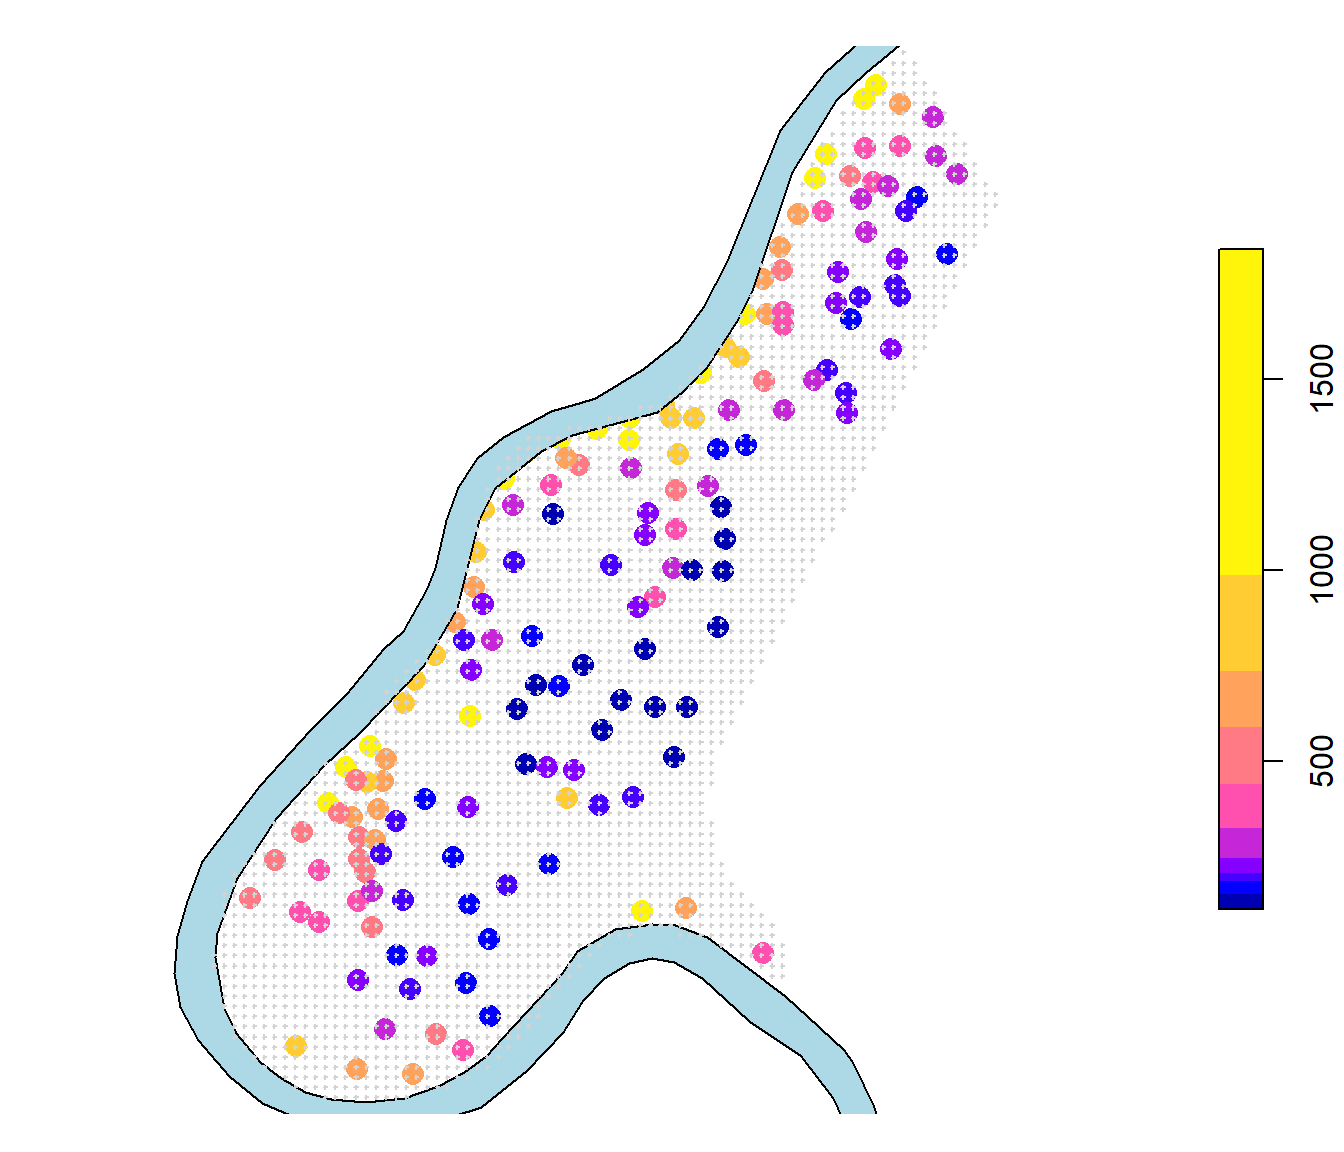
\includegraphics[width=0.7\linewidth]{02-datos_files/figure-latex/meuse-sf-1} 

}

\caption{Concentración de zinc (ppm) en el entorno del río Meuse (datos `sp::meuse`).}\label{fig:meuse-sf}
\end{figure}

\hypertarget{crs}{%
\subsection{Sistemas de referencia de coordenadas}\label{crs}}

El sistema de referencia de coordenadas (CRS) especifica la correspondencia entre valores de las coordenadas y puntos concretos en la superficie de la Tierra (o del espacio), y resulta fundamental cuando se combinan datos espaciales.
En general se consideran dos tipos de CRS:

\begin{itemize}
\item
  Geodésico: las coordenadas en tres dimensiones (latitud, longitud y altura) se basan en un elipsoide de referencia (global o local) que sirve como aproximación del globo terrestre (se tiene en cuenta que no es una esfera perfecta e incluso que puede haber variaciones locales). Este elipsoide, junto con información adicional sobre como interpretar las coordenadas (incluyendo el orden y el origen), define el denominado \emph{datum}. Normalmente se asume que las coordenadas son en la superficie terrestre y solo se consideran:

  \begin{itemize}
  \tightlist
  \item
    latitud: ángulo entre el plano ecuatorial y la línea que une la posición con el centro de la Tierra. Varía desde -90 (polo sur) hasta 90 (polo norte). Un grado equivale aproximadamente a 110.6 km. Los paralelos son las líneas en la superficie terrestre correspondientes a la misma latitud (siendo el 0 el ecuador).
  \item
    longitud: ángulo (paralelo al plano ecuatorial) entre un meridiano de referencia (arco máximo que une los polos pasando por una determinado punto, normalmente el observatorio de Greenwich) y la línea que une la posición con el centro de la Tierra. Varía desde -180 (oeste) hasta 180 (este). Un grado en el ecuador equivale a aproximadamente a 111.3 km. Los meridianos son las líneas en la superficie terrestre correspondientes a la misma longitud (siendo el 0 el meridiano de Greenwich y -180 o 180 el correspondiente antimeridiano).
  \end{itemize}

  La rejilla correspondiente a un conjunto de paralelos y meridianos se denomina \emph{gratícula} (ver \texttt{st\_graticule()}).

  \begin{figure}[!htb]

    {\centering 
\includegraphics[width=0.85\linewidth]{images/Latitud_y_Longitud} 

    }

    \caption{Coordenadas geográficas en la superficie terrestre (Fuente Wikimedia Commons).}\label{fig:latlon}
    \end{figure}

  Uno de los CRS más empleados es el WGS84 (\emph{World Geodetic System 1984}) en el que se basa el \emph{Sistema de Posicionamiento Global} (GPS).
\item
  Proyectado (cartesiano): sistema (local) en dos dimensiones que facilita algún tipo de cálculo (normalmente distancias o áreas). Por ejemplo el UTM (\emph{Universal Transverse Mercator}), que emplea coordenadas en metros respecto a una cuadrícula de referencia (se divide la tierra en 60 husos de longitud, numerados, y 20 bandas de latitud, etiquetadas con letras; por ejemplo Galicia se encuentra en la cuadricula 29T). Se define relacionando estas coordenadas cartesianas con coordenadas geodésicas con un determinado datum.
\end{itemize}

En \texttt{sf} se emplea la librería \href{http://proj.org/}{PRØJ} para definir el CRS y convertir coordenadas en distintos sistemas\footnote{El paquete \texttt{sf} admite las últimas versiones PROJ 5 y 6, incluyendo el formato WKT-2 de 2019, mientras que el paquete \texttt{sp} está diseñado para cadenas \emph{PROJ.4 string} que se recomiendan abandonar (las últimas versiones permiten añadir una cadena WKT2 como \texttt{comment}).}.
Para obtener o establecer el CRS se puede emplear la función \texttt{st\_crs()}.
Se puede especificar mediante una cadena de texto que admita \href{https://gdal.org/tutorials/osr_api_tut.html}{GDAL} (por ejemplo \texttt{"WGS84"}, que se corresponde con el \emph{World Geodetic System 1984}), que típicamente es de la forma ESTÁNDAR:CÓDIGO.
El estándar más empleado es el \href{https://epsg.org}{EPSG} (\emph{European Petroleum Survey Group}), y es que que da por hecho el paquete \texttt{sf} cuando se especifica el CRS mediante un número.
También admite el estándar \href{http://www.opengeospatial.org/standards/wkt-crs}{OGC WKT} (\emph{Open Geospatial Consortium well-known text}) que es el que emplea internamente, pero resulta complicado manejar en la práctica.

\begin{Shaded}
\begin{Highlighting}[]
\FunctionTok{st\_crs}\NormalTok{(}\StringTok{"WGS84"}\NormalTok{)}
\end{Highlighting}
\end{Shaded}

\begin{verbatim}
## Coordinate Reference System:
##   User input: WGS84 
##   wkt:
## GEOGCRS["WGS 84",
##     DATUM["World Geodetic System 1984",
##         ELLIPSOID["WGS 84",6378137,298.257223563,
##             LENGTHUNIT["metre",1]]],
##     PRIMEM["Greenwich",0,
##         ANGLEUNIT["degree",0.0174532925199433]],
##     CS[ellipsoidal,2],
##         AXIS["geodetic latitude (Lat)",north,
##             ORDER[1],
##             ANGLEUNIT["degree",0.0174532925199433]],
##         AXIS["geodetic longitude (Lon)",east,
##             ORDER[2],
##             ANGLEUNIT["degree",0.0174532925199433]],
##     ID["EPSG",4326]]
\end{verbatim}

\begin{Shaded}
\begin{Highlighting}[]
\FunctionTok{all.equal}\NormalTok{(}\FunctionTok{st\_crs}\NormalTok{(}\DecValTok{4326}\NormalTok{), }\FunctionTok{st\_crs}\NormalTok{(}\StringTok{"EPSG:4326"}\NormalTok{), }\FunctionTok{st\_crs}\NormalTok{(}\StringTok{"WGS84"}\NormalTok{))}
\end{Highlighting}
\end{Shaded}

\begin{verbatim}
## [1] TRUE
\end{verbatim}

\begin{Shaded}
\begin{Highlighting}[]
\FunctionTok{st\_crs}\NormalTok{(nc)}
\end{Highlighting}
\end{Shaded}

\begin{verbatim}
## Coordinate Reference System:
##   User input: NAD27 
##   wkt:
## GEOGCRS["NAD27",
##     DATUM["North American Datum 1927",
##         ELLIPSOID["Clarke 1866",6378206.4,294.978698213898,
##             LENGTHUNIT["metre",1]]],
##     PRIMEM["Greenwich",0,
##         ANGLEUNIT["degree",0.0174532925199433]],
##     CS[ellipsoidal,2],
##         AXIS["latitude",north,
##             ORDER[1],
##             ANGLEUNIT["degree",0.0174532925199433]],
##         AXIS["longitude",east,
##             ORDER[2],
##             ANGLEUNIT["degree",0.0174532925199433]],
##     ID["EPSG",4267]]
\end{verbatim}

En \href{https://spatialreference.org}{spatialreference.org} se puede obtener información detallada sobre una gran cantidad de proyecciones (y permite realizar búsquedas).
También puede ser de utilidad \href{https://epsg.io}{epsg.io} o este \href{https://proj.org/operations/projections}{listado} con detalles de los parámetros.

El CRS ideal dependerá del tipo de problema y de la zona cubierta por los datos (ver e.g Lovelace et al, 2021, \href{https://geocompr.robinlovelace.net/reproj-geo-data.html\#which-crs-to-use}{Sección 6.3}, para más información).
En general en estadística espacial nos interesará trabajar con coordenadas proyectadas, de forma que tenga sentido emplear la distancia euclídea (algo que puede ser poco o nada razonable si se trabaja con coordenadas geodésicas en una zona muy amplia del globo o cerca de los polos).
En el caso de coordenadas sin proyectar (latitud/longitud) puede ser preferible trabajar con distancias ortodrómicas (longitud del arco del círculo máximo que une los puntos, \emph{great circle distances})\footnote{Algo que ya hace de forma automática el paquete \texttt{gstat}.}.
Es importante destacar que cambiar el CRS no reproyecta los datos, hay que emplear \texttt{st\_transform()} para hacerlo, como se describe en la Sección \ref{operaciones-datos}.

Finalmente hay que insistir también en que el campo de aplicación de la estadística espacial no se restringe al análisis de datos geográficos (por ejemplo nos puede interesar analizar el desgaste en la pared de un crisol empleado en fundición) y en estos casos los CRS geográficos carecen de sentido.
De todos modos habrá que emplear un sistema de coordenadas que permita calcular algún tipo de salto o distancia entre puntos (aunque siempre se pueden considerar coordenadas espaciales tres dimensiones con la distancia euclídea).

\hypertarget{tidyverse-sf}{%
\subsection{\texorpdfstring{Integración con el ecosistema \textbf{tidyverse}}{Integración con el ecosistema tidyverse}}\label{tidyverse-sf}}

El paquete \texttt{sf} es compatible con \href{http://tidyverse.org}{\texttt{tidyverse}} y proporciona métodos para interactuar con los paquetes \href{https://dplyr.tidyverse.org}{\texttt{dplyr}},
\href{http://tidyr.tidyverse.org}{\texttt{tidyr}} y \href{https://ggplot2.tidyverse.org}{\texttt{ggplot2}}.

Algunos de los métodos de interés para manipular datos espaciales con el paquete \href{https://dplyr.tidyverse.org}{\texttt{dplyr}} son:

\begin{itemize}
\tightlist
\item
  \texttt{filter()}, \texttt{select()}, \texttt{mutate()}, \texttt{summarise(...,\ do\_union\ =\ TRUE,\ is\_coverage\ =\ FALSE)}, \texttt{group\_by()}, \texttt{ungroup()}, etc.
\item
  \texttt{inner\_join()}, \texttt{left\_join()}, \texttt{right\_join()}, \texttt{full\_join()}, \texttt{semi\_join()}, \texttt{anti\_join()}, \texttt{st\_join()}.
\item
  \texttt{st\_drop\_geometry()}, \texttt{st\_set\_crs()}.
\end{itemize}

Para detalles ver la \href{https://r-spatial.github.io/sf/reference/tidyverse.html}{referencia}.

En el caso del paquete \href{https://ggplot2.tidyverse.org}{\texttt{ggplot2}} se puede consultar la \href{https://ggplot2.tidyverse.org/reference/ggsf.html}{referencia} y el tutorial \emph{Drawing beautiful maps programmatically with R, sf and ggplot2}:

\begin{itemize}
\tightlist
\item
  \href{https://r-spatial.org/r/2018/10/25/ggplot2-sf.html}{Part 1: Basics (General concepts illustrated with the world Map)}.
\item
  \href{https://r-spatial.org/r/2018/10/25/ggplot2-sf-2.html}{Part 2: Layers (Adding additional layers: an example with points and polygons)}.
\item
  \href{https://r-spatial.org/r/2018/10/25/ggplot2-sf-3.html}{Part 3: Layouts (Positioning and layout for complex maps)}.
\end{itemize}

Por ejemplo, se puede generar un gráfico similar al de la Figura \ref{fig:mortalidad} (porcentaje de incremento de las defunciones en el año 2020 respecto al 2019 en las CCAA españolas; datos provisionales \href{https://www.ine.es/jaxi/Tabla.htm?tpx=21856\&L=0}{INE}), con el siguiente código:

\begin{Shaded}
\begin{Highlighting}[]
\FunctionTok{library}\NormalTok{(dplyr)}
\FunctionTok{library}\NormalTok{(mapSpain) }
\NormalTok{mortalidad }\OtherTok{\textless{}{-}} \FunctionTok{read.csv2}\NormalTok{(}\StringTok{"datos/mortalidad.csv"}\NormalTok{)}
\NormalTok{CCAA\_sf }\OtherTok{\textless{}{-}} \FunctionTok{esp\_get\_ccaa}\NormalTok{() }\SpecialCharTok{\%\textgreater{}\%} \FunctionTok{left\_join}\NormalTok{(mortalidad) }\SpecialCharTok{\%\textgreater{}\%}
  \FunctionTok{mutate}\NormalTok{(}\AttributeTok{incremento =} \DecValTok{100}\SpecialCharTok{*}\NormalTok{(mort}\FloatTok{.2020} \SpecialCharTok{{-}}\NormalTok{ mort}\FloatTok{.2019}\NormalTok{)}\SpecialCharTok{/}\NormalTok{mort}\FloatTok{.2019}\NormalTok{)}

\FunctionTok{library}\NormalTok{(ggplot2)}
\FunctionTok{ggplot}\NormalTok{(CCAA\_sf) }\SpecialCharTok{+}
  \FunctionTok{geom\_sf}\NormalTok{(}\FunctionTok{aes}\NormalTok{(}\AttributeTok{fill =}\NormalTok{ incremento), }\AttributeTok{color =} \StringTok{"grey70"}\NormalTok{) }\SpecialCharTok{+}
  \FunctionTok{scale\_fill\_gradientn}\NormalTok{(}\AttributeTok{colors =} \FunctionTok{hcl.colors}\NormalTok{(}\DecValTok{10}\NormalTok{, }\StringTok{"Blues"}\NormalTok{, }\AttributeTok{rev =} \ConstantTok{TRUE}\NormalTok{)) }\SpecialCharTok{+}
  \FunctionTok{geom\_sf\_label}\NormalTok{(}\FunctionTok{aes}\NormalTok{(}\AttributeTok{label =} \FunctionTok{paste0}\NormalTok{(}\FunctionTok{round}\NormalTok{(incremento, }\DecValTok{1}\NormalTok{), }\StringTok{"\%"}\NormalTok{)), }\AttributeTok{alpha =} \FloatTok{0.5}\NormalTok{) }\SpecialCharTok{+}
  \FunctionTok{geom\_sf}\NormalTok{(}\AttributeTok{data =} \FunctionTok{esp\_get\_can\_box}\NormalTok{(), }\AttributeTok{color =} \StringTok{"grey70"}\NormalTok{) }\SpecialCharTok{+} 
  \FunctionTok{theme\_void}\NormalTok{()}
\end{Highlighting}
\end{Shaded}

\begin{figure}[!htb]

{\centering 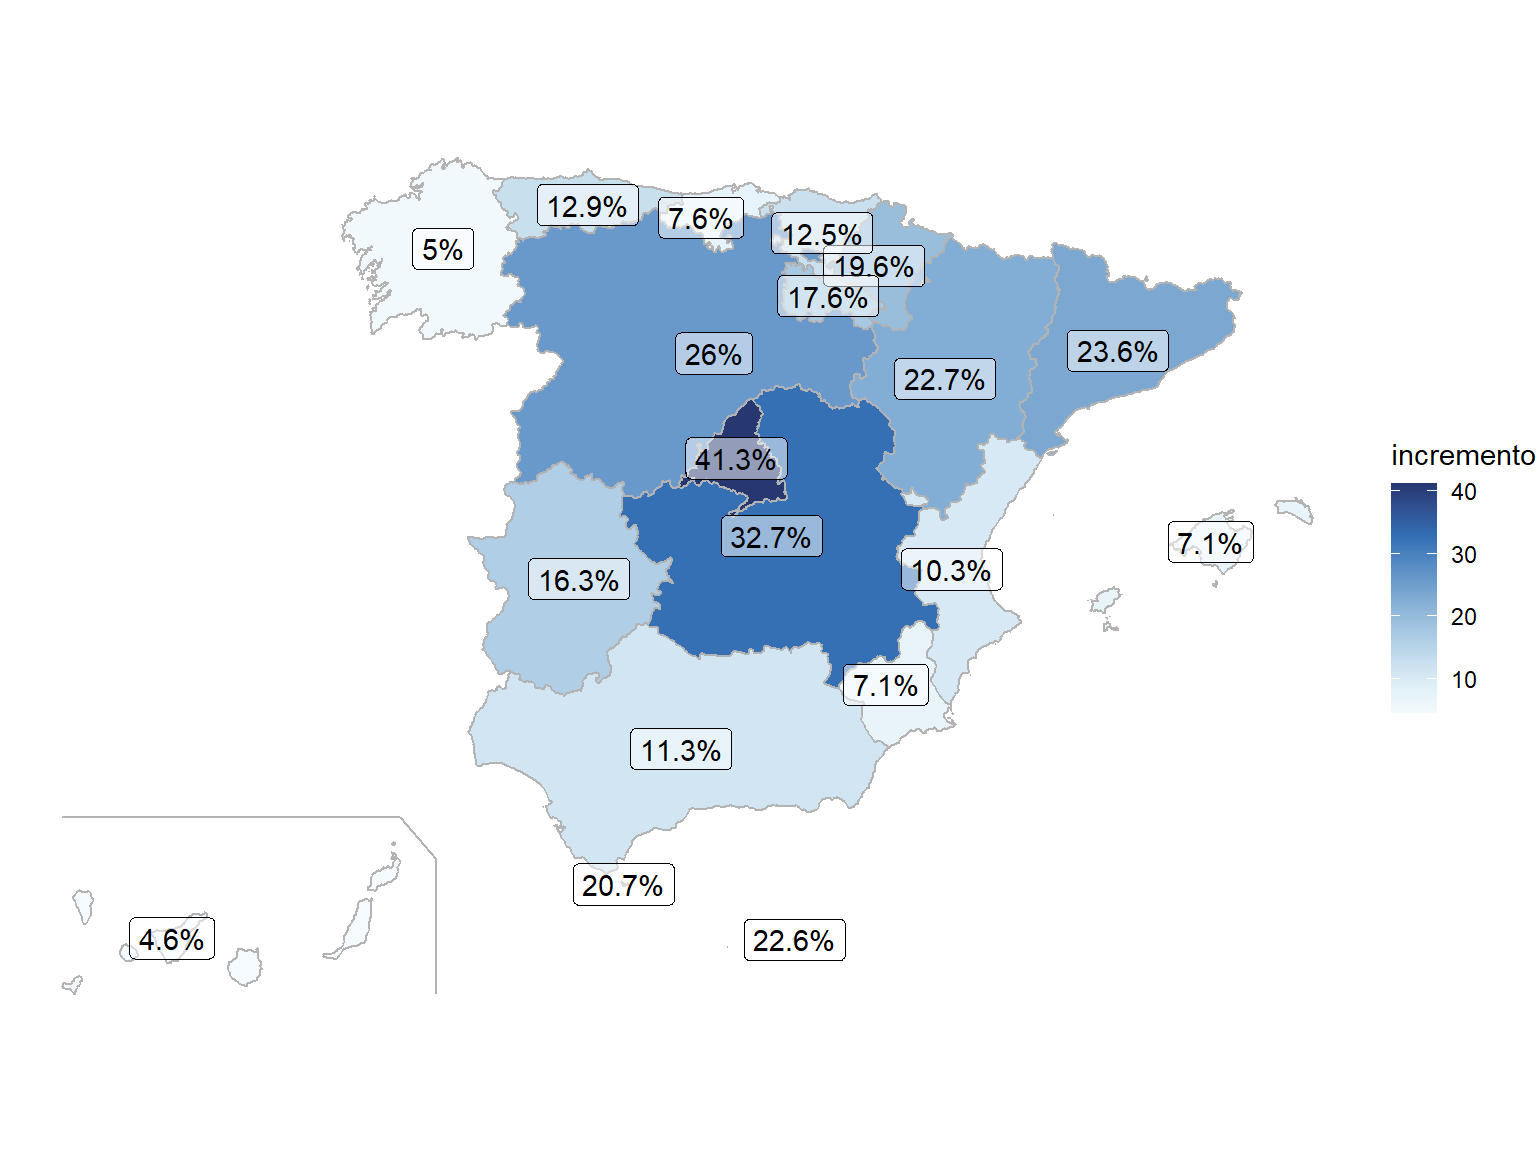
\includegraphics[width=0.7\linewidth]{02-datos_files/figure-latex/dplyr-ggplot-1} 

}

\caption{Ejemplo de gráfico generado empleando los paquetes `dplyr` y `ggplot2`.}\label{fig:dplyr-ggplot}
\end{figure}

{[}Figura \ref{fig:dplyr-ggplot}{]}

Sin embargo, en estos apuntes se supone que no se está familiarizado con estas herramientas y se evitará su uso (aunque pueden resultar más cómodas después de su aprendizaje).
Para una introducción a \href{https://dplyr.tidyverse.org}{\texttt{dplyr}}, ver por ejemplo la viñeta \href{https://cran.rstudio.com/web/packages/dplyr/vignettes/dplyr.html}{Introduction to dplyr},
el \href{http://r4ds.had.co.nz/transform.html}{Capítulo 5} del libro \href{http://r4ds.had.co.nz}{R for Data Science} o el \href{https://gltaboada.github.io/tgdbook/dplyr.html}{Capítulo 4} de los apuntes \href{https://gltaboada.github.io/tgdbook}{Prácticas de Tecnologías de Gestión y Manipulación de Datos}.

No obstante, en ciertas ocasiones emplearemos el operador \emph{pipe} \texttt{\%\textgreater{}\%} (tubería, redirección) por comodidad.
Este operador permite canalizar la salida de una función a la entrada de otra.
Por ejemplo \texttt{segundo(primero(datos))} se traduce en \texttt{datos\ \%\textgreater{}\%\ primero\ \%\textgreater{}\%\ segundo}
(facilitando la lectura de expresiones de izquierda a derecha).

\hypertarget{representaciuxf3n-de-datos-espaciales}{%
\section{Representación de datos espaciales}\label{representaciuxf3n-de-datos-espaciales}}

El paquete \texttt{sf} implementa métodos \texttt{plot()} para la representación de objetos espaciales (ver \href{https://r-spatial.github.io/sf/reference/plot.html}{\texttt{?plot.sf}}).
Estos métodos suelen ser la forma más rápida de generar gráficos básicos (estáticos), pero también se pueden emplear otros paquetes como \href{https://ggplot2.tidyverse.org}{\texttt{ggplot2}} (Sección \ref{tidyverse-sf}), \href{https://r-tmap.github.io/tmap}{\texttt{tmap}}, \href{https://riatelab.github.io/mapsf}{\texttt{mapsf}}, \href{https://rstudio.github.io/leaflet}{\texttt{leaflet}}, \href{https://r-spatial.github.io/mapview}{\texttt{mapview}}, \href{https://symbolixau.github.io/mapdeck}{\texttt{mapdeck}} o \href{https://github.com/dkahle/ggmap}{\texttt{ggmap}}, para generar mapas más avanzados, incluyendo mapas dinámicos.
Para una introducción a las posibilidades gráficas con el paquete \texttt{sf} se puede consultar la viñeta \href{https://r-spatial.github.io/sf/articles/sf5.html}{\emph{Plotting Simple Features}}.

El método \texttt{plot()} es de la forma:

\begin{Shaded}
\begin{Highlighting}[]
\FunctionTok{plot}\NormalTok{(x, ..., max.plot, }\AttributeTok{pal =} \ConstantTok{NULL}\NormalTok{, nbreaks, }\AttributeTok{breaks =} \StringTok{"pretty"}\NormalTok{, }
\NormalTok{     key.pos, key.length, key.width, }\AttributeTok{extent =}\NormalTok{ x, }\AttributeTok{axes =} \ConstantTok{FALSE}\NormalTok{, }
     \AttributeTok{graticule =}\NormalTok{ NA\_crs\_, }\AttributeTok{col\_graticule =} \StringTok{"grey"}\NormalTok{, border, }\AttributeTok{reset =} \ConstantTok{TRUE}\NormalTok{)}
\end{Highlighting}
\end{Shaded}

\begin{itemize}
\tightlist
\item
  \texttt{x}: objeto de tipo \texttt{sf} o \texttt{sfc}.
\item
  \texttt{max.plot}: número máximo de atributos que se representarán.
\item
  \texttt{pal}: función que genera la paleta de colores (ver e.g.~\texttt{?rainbow}), por defecto \texttt{sf.colors} (ver Figura \ref{fig:multi-plot-sf}).
\item
  \texttt{nbreaks}: número de puntos de corte para la clave de color.
\item
  \texttt{breaks}: vector de puntos de corte o cadena de texto válida para el argumento \texttt{style} de \texttt{classIntervals} (ver figuras: \ref{fig:meuse-sf}, \ref{fig:multi-plot-sf}).
\item
  \texttt{key.pos}: posición de la leyenda, -1 = automática, 0 = error?, 1 = abajo, 2 = izquierda, 3 = arriba, 4 = derecha, NULL = omitir. Cuando se representan múltiples atributos se añade una única leyenda común únicamente si se establece (ver figuras: \ref{fig:multi-plot-sf}, \ref{fig:transform}).
\item
  \texttt{key.length}, \texttt{key.width}: dimensiones de la leyenda (proporción de espacio).
\item
  \texttt{extent}: objeto con método \texttt{st\_bbox()} para definir los límites (sustituyendo a \texttt{xlim} e \texttt{ylim}).
\item
  \texttt{axes}: lógico; \texttt{TRUE} para dibujar los ejes.
\item
  \texttt{graticule}: lógico, objeto de clase \texttt{crs} (\texttt{st\_crs()}) u objeto creado por \texttt{st\_graticule}; \texttt{TRUE} representará la gratícula \texttt{st\_graticule(x)} (ver Figura \ref{fig:transform}).
\item
  \texttt{col\_graticule}: color de la gratícula.
\item
  \texttt{border}: color de los bordes de polígonos.
\item
  \texttt{reset}: lógico; si el gráfico contiene una leyenda se modifican los parámetros gráficos y por defecto los restaura (\texttt{reset\ =\ TRUE}). Solo en ese caso es necesario establecer \texttt{reset\ =\ FALSE} para continuar añadiendo elementos, con \texttt{add\ =\ TRUE} (para restaurarlos hay que ejecutar \texttt{dev.off()}) (ver figuras: \ref{fig:meuse-sf}, \ref{fig:multi-plot-sf}).
\item
  \texttt{...}: otros parámetros gráficos (ver \texttt{?plot.default} y \texttt{?par}).
\end{itemize}

Ejemplo:

\begin{Shaded}
\begin{Highlighting}[]
\FunctionTok{library}\NormalTok{(viridis)}
\FunctionTok{plot}\NormalTok{(nc[}\FunctionTok{c}\NormalTok{(}\StringTok{"SID74"}\NormalTok{, }\StringTok{"SID79"}\NormalTok{)], }\AttributeTok{pal =}\NormalTok{ viridis, }\AttributeTok{border =} \StringTok{\textquotesingle{}grey70\textquotesingle{}}\NormalTok{, }\AttributeTok{logz =} \ConstantTok{TRUE}\NormalTok{, }
     \AttributeTok{breaks =} \FunctionTok{seq}\NormalTok{(}\DecValTok{0}\NormalTok{, }\DecValTok{2}\NormalTok{, }\AttributeTok{len =} \DecValTok{9}\NormalTok{), }\AttributeTok{at =} \FunctionTok{c}\NormalTok{(}\DecValTok{0}\NormalTok{, }\FloatTok{0.5}\NormalTok{, }\DecValTok{1}\NormalTok{, }\FloatTok{1.5}\NormalTok{, }\DecValTok{2}\NormalTok{), }
     \AttributeTok{key.pos =} \DecValTok{1}\NormalTok{, }\AttributeTok{key.width =} \FunctionTok{lcm}\NormalTok{(}\FloatTok{1.2}\NormalTok{), }\AttributeTok{key.length =} \FloatTok{0.8}\NormalTok{) }
\end{Highlighting}
\end{Shaded}

\begin{figure}[!htb]

{\centering 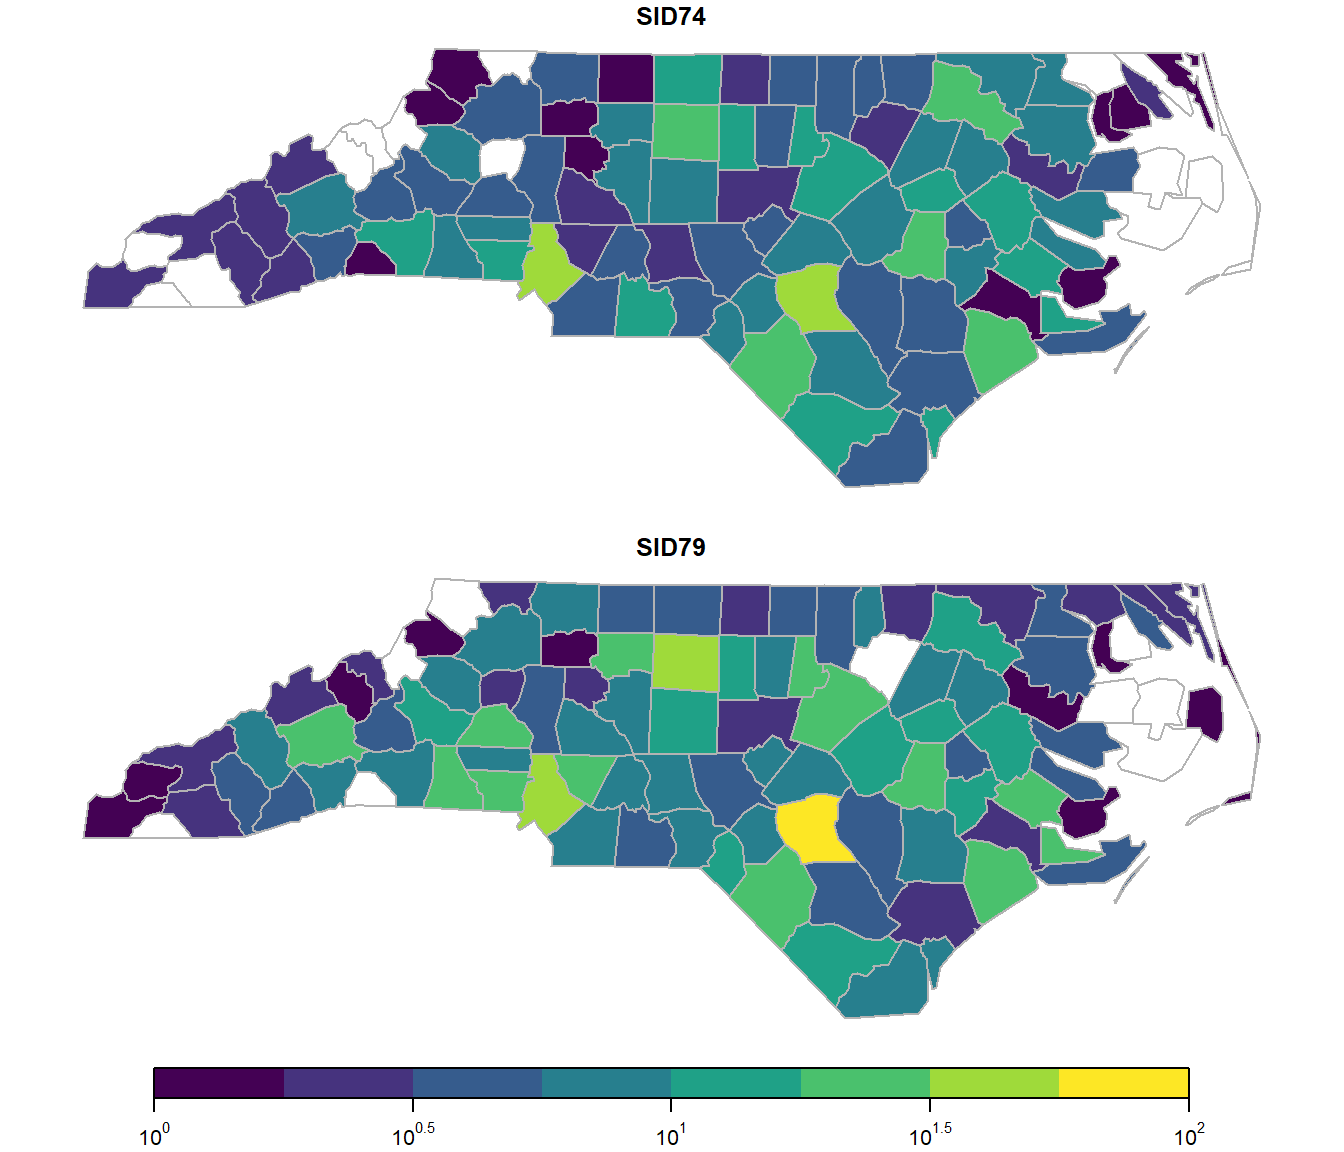
\includegraphics[width=0.7\linewidth]{02-datos_files/figure-latex/multi-plot-sf-1} 

}

\caption{Ejemplo de gráfico con múltiples atributos (con colores personalizados y leyenda común, en escala logarítmica personalizada).}\label{fig:multi-plot-sf}
\end{figure}

El paquete \href{https://r-tmap.github.io/tmap}{\texttt{tmap}} permite generar mapas temáticos con una gramática similar a la de \texttt{ggplot2} pero enfocada a mapas.
Por defecto crea mapas estáticos (\texttt{tmap\_mode("plot")}):

\begin{Shaded}
\begin{Highlighting}[]
\FunctionTok{library}\NormalTok{(tmap)}
\FunctionTok{tm\_shape}\NormalTok{(nc) }\SpecialCharTok{+} \FunctionTok{tm\_polygons}\NormalTok{(}\StringTok{"SID79"}\NormalTok{)}
\end{Highlighting}
\end{Shaded}

\begin{figure}[!htb]

{\centering 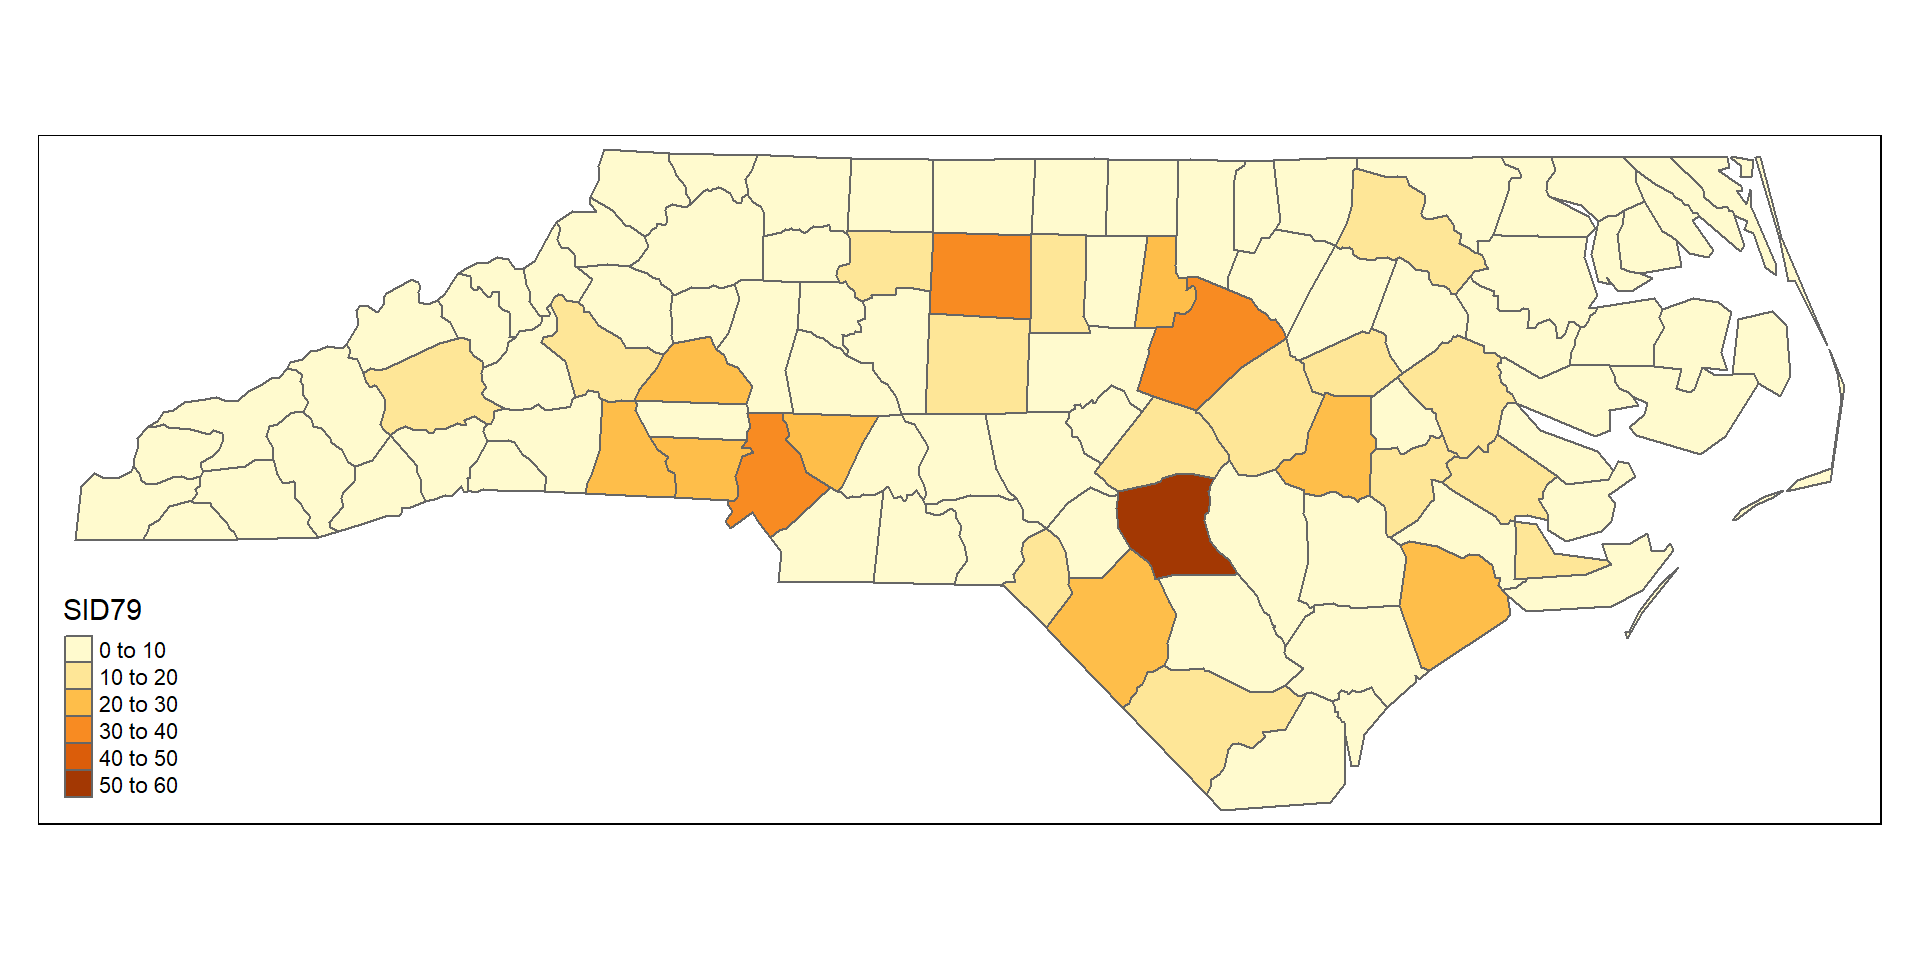
\includegraphics[width=0.7\linewidth]{02-datos_files/figure-latex/tmap-plot-1} 

}

\caption{Ejemplo de mapa estático creado con `tmap`.}\label{fig:tmap-plot}
\end{figure}

Aunque puede crear mapas interactivos, en páginas html, utilizando el paquete \href{https://rstudio.github.io/leaflet}{\texttt{leaflet}} (interfaz a la librería JavaScript \href{https://leafletjs.com}{Leaflet}), implementando también leyendas, ventanas emergentes al pulsar con el ratón en las características y soporte para datos rasterizados.

\begin{Shaded}
\begin{Highlighting}[]
\FunctionTok{tmap\_mode}\NormalTok{(}\StringTok{"view"}\NormalTok{)}
\FunctionTok{tmap\_last}\NormalTok{()}
\CommentTok{\# Error en bookdown}
\end{Highlighting}
\end{Shaded}

Para más información ver el capítulo \href{https://geocompr.robinlovelace.net/adv-map.html\#adv-map}{Making maps with R} del libro \href{https://geocompr.robinlovelace.net}{Geocomputation with R}, la \href{https://r-tmap.github.io/tmap/articles/tmap-getstarted.html}{viñeta} del paquete, o el borrador del libro \href{https://r-tmap.github.io}{Elegant and informative maps with tmap}.

El paquete \href{https://r-spatial.github.io/mapview}{\texttt{mapview}} también permite crear mapas interactivos utilizando el paquete \href{https://rstudio.github.io/leaflet}{\texttt{leaflet}} (con funcionalidades añadidas) o el paquete \href{https://symbolixau.github.io/mapdeck}{\texttt{mapdeck}} (diseñado para grandes conjuntos de datos espaciales).

\begin{Shaded}
\begin{Highlighting}[]
\FunctionTok{library}\NormalTok{(mapview)}
\FunctionTok{mapview}\NormalTok{(nc, }\AttributeTok{zcol =} \StringTok{"SID79"}\NormalTok{)}
\CommentTok{\# Error en bookdown}
\end{Highlighting}
\end{Shaded}

Para más información ver las \href{https://r-spatial.github.io/mapview/articles/articles/mapview_01-basics.html}{viñetas} del paquete.

\hypertarget{operaciones-datos}{%
\section{Operaciones con datos espaciales}\label{operaciones-datos}}

A continuación se describe una selección de las herramientas disponibles para datos espaciales.
Para un listado completo de las funciones implementadas en el paquete \texttt{sf} se puede consultar la \href{https://r-spatial.github.io/sf/reference/index.html}{referencia} (o la ``\href{https://github.com/rstudio/cheatsheets/blob/master/sf.pdf}{chuleta}'', aunque puede contener algunos errores).

Puede que algunas herramientas (o recursos) admitan únicamente objetos \texttt{Spatial*} del paquete \texttt{sp}, aunque siempre se pueden emplear las funciones para convertir tipos de objetos:

\begin{itemize}
\tightlist
\item
  \texttt{st\_as\_sf(x,\ ...)}: convierte \texttt{x} a un objeto \texttt{sf} (por ejemplo objetos \texttt{Spatial*}).
\item
  \texttt{as(x,\ "Spatial")}: convierte \texttt{x} a un objeto \texttt{Spatial*}.
\end{itemize}

\hypertarget{importaciuxf3n-y-exportaciuxf3n-de-datos-espaciales}{%
\subsection{Importación y exportación de datos espaciales}\label{importaciuxf3n-y-exportaciuxf3n-de-datos-espaciales}}

El paquete \texttt{sf} permite importar y exportar una gran cantidad de formatos de datos espaciales, almacenados en ficheros o en bases de datos, mediante las funciones \texttt{st\_read()} y \texttt{st\_write()}.
Como se mostró al principio de la Sección \ref{sf-intro}, estas funciones deducen el formato automáticamente a partir de la extensión del archivo:

\begin{Shaded}
\begin{Highlighting}[]
\NormalTok{dir }\OtherTok{\textless{}{-}} \FunctionTok{system.file}\NormalTok{(}\StringTok{"shape"}\NormalTok{, }\AttributeTok{package=}\StringTok{"sf"}\NormalTok{)}
\FunctionTok{list.files}\NormalTok{(dir, }\AttributeTok{pattern=}\StringTok{"\^{}[nc]"}\NormalTok{)}
\end{Highlighting}
\end{Shaded}

\begin{verbatim}
## [1] "nc.dbf" "nc.prj" "nc.shp" "nc.shx"
\end{verbatim}

\begin{Shaded}
\begin{Highlighting}[]
\CommentTok{\# ESRI Shapefile, consta por lo menos de 3 ficheros, el principal .shp}
\NormalTok{file }\OtherTok{\textless{}{-}} \FunctionTok{paste0}\NormalTok{(dir, }\StringTok{"/nc.shp"}\NormalTok{)}
\NormalTok{file}
\end{Highlighting}
\end{Shaded}

\begin{verbatim}
## [1] "C:/Program Files/R/R-4.1.0/library/sf/shape/nc.shp"
\end{verbatim}

\begin{Shaded}
\begin{Highlighting}[]
\NormalTok{nc\_sf }\OtherTok{\textless{}{-}} \FunctionTok{st\_read}\NormalTok{(file)}
\end{Highlighting}
\end{Shaded}

\begin{verbatim}
## Reading layer `nc' from data source 
##   `C:\Program Files\R\R-4.1.0\library\sf\shape\nc.shp' using driver `ESRI Shapefile'
## Simple feature collection with 100 features and 14 fields
## Geometry type: MULTIPOLYGON
## Dimension:     XY
## Bounding box:  xmin: -84.32385 ymin: 33.88199 xmax: -75.45698 ymax: 36.58965
## Geodetic CRS:  NAD27
\end{verbatim}

Se admiten los formatos de datos vectoriales \href{https://gdal.org/drivers/vector/index.html}{soportados por GDAL} (que emplea internamente),
se puede obtener un listado con la función \texttt{st\_drivers()}:

\begin{Shaded}
\begin{Highlighting}[]
\NormalTok{drivers }\OtherTok{\textless{}{-}} \FunctionTok{st\_drivers}\NormalTok{()}
\FunctionTok{str}\NormalTok{(drivers)}
\end{Highlighting}
\end{Shaded}

\begin{verbatim}
## 'data.frame':    89 obs. of  7 variables:
##  $ name     : chr  "ESRIC" "FITS" "PCIDSK" "netCDF" ...
##  $ long_name: chr  "Esri Compact Cache" "Flexible Image Transport System" "PCIDSK Database File" "Network Common Data Format" ...
##  $ write    : logi  FALSE TRUE TRUE TRUE TRUE TRUE ...
##  $ copy     : logi  FALSE FALSE FALSE TRUE TRUE TRUE ...
##  $ is_raster: logi  TRUE TRUE TRUE TRUE TRUE TRUE ...
##  $ is_vector: logi  TRUE TRUE TRUE TRUE TRUE TRUE ...
##  $ vsi      : logi  TRUE FALSE TRUE FALSE TRUE TRUE ...
\end{verbatim}

Además, se han desarrollado una gran cantidad de paquetes de R que permiten acceder directamente desde R a datos espaciales.
Muchos incluyen conjuntos de datos espaciales y otros implementan interfaces a bases de datos espaciales o geoportales disponibles en Internet.
Algunos de ellos son los siguientes:

\begin{itemize}
\tightlist
\item
  \href{https://docs.ropensci.org/rnaturalearth/}{\texttt{rnaturalearth}}: permite importar una gran cantidad de datos vectoriales y rasterizados de \href{http://www.naturalearthdata.com}{Natural Earth}, incluyendo datos administrativos/culturales (fronteras de países, aeropuertos, carreteras, vías férreas\ldots) y físicos (costas, lagos\ldots).
\item
  \href{https://ec.europa.eu/eurostat/web/gisco}{\texttt{giscoR}}: permite importar datos de \href{}{Eurostat - GISCO} (\emph{Geographic Information System of the COmmission}).
\item
  \href{https://ropenspain.github.io/mapSpain}{\texttt{mapSpain}}: permite importar límites administrativos de España (CCAA, provincias, municipios\ldots).
\item
  \href{https://CRAN.R-project.org/package=osmdata}{\texttt{osmdata}}: permite importar ``pequeños'' conjuntos de datos de \href{https://www.openstreetmap.org}{OpenStreetMap} (OSM).
\item
  \href{https://CRAN.R-project.org/package=osmextract}{\texttt{osmextract}}: permite importar grandes conjuntos de datos de OSM.
\item
  \href{https://github.com/eblondel/ows4R/wiki}{\texttt{ows4R}}: (en desarrollo) proporciona una interfaz para \emph{\href{https://www.ogc.org/docs/is}{OGC standard Web-Services}} (OWS).
\item
  \href{https://open-eo.github.io/openeo-r-client}{\texttt{openeo}}: permite importar datos de servidores \href{https://openeo.org}{openEO} (\emph{Open Earth Observation data}).
\item
  \href{https://CRAN.R-project.org/package=rnoaa}{\texttt{rnoaa}}: permite importar datos climáticos de la \href{https://www.ncdc.noaa.gov/cdo-web/webservices/v2}{National Oceanic and Atmospheric Administration} (NOAA).
\item
  \href{https://ropenspain.github.io/climaemet}{\texttt{climaemet}}: permite importar datos climáticos proporcionados por la \href{https://opendata.aemet.es}{Agencia Estatal de Meteorología de España} (AEMET).
\item
  \href{https://github.com/oscarperpinan/meteoForecast}{\texttt{meteoForecast}}: permite importar resultados de los modelos numéricos de predicción meteorológica \href{https://www.ncdc.noaa.gov/data-access/model-data/model-datasets/global-forcast-system-gfs}{GFS},
  \href{https://www.meteogalicia.gal/web/modelos/threddsIndex.action}{MeteoGalicia}, \href{https://www.ncdc.noaa.gov/data-access/model-data/model-datasets/north-american-mesoscale-forecast-system-nam}{NAM} y \href{https://www.ncdc.noaa.gov/data-access/model-data/model-datasets/rapid-refresh-rap}{RAP}.
\item
  \href{https://github.com/skgrange/saqgetr}{\texttt{saqgetr}}: permite importar datos de calidad del aire de Europa.
\item
  \href{https://github.com/spatialstatisticsupna/RGISTools}{\texttt{RGISTools}}: permite importar datos de imágenes de satélite de Landsat, MODIS y Sentinel.
\item
  \href{https://CRAN.R-project.org/package=maptools}{\texttt{maptools}},\href{https://CRAN.R-project.org/package=spData}{\texttt{spData}},\href{https://CRAN.R-project.org/package=spDataLarge}{\texttt{spDataLarge}},\href{https://CRAN.R-project.org/package=getlandsat}{\texttt{getlandsat}}\ldots{}
\end{itemize}

\begin{Shaded}
\begin{Highlighting}[]
\FunctionTok{library}\NormalTok{(osmdata) }
\CommentTok{\# Cuidado: descarga mucha información}
\CommentTok{\# https://nominatim.openstreetmap.org/ui/search.html}
\CommentTok{\# https://wiki.openstreetmap.org/wiki/Map\_features}
\NormalTok{osm\_coru }\OtherTok{\textless{}{-}} \FunctionTok{opq}\NormalTok{(}\StringTok{\textquotesingle{}A Coruña\textquotesingle{}}\NormalTok{) }\SpecialCharTok{\%\textgreater{}\%}
    \FunctionTok{add\_osm\_feature}\NormalTok{(}\AttributeTok{key =} \StringTok{\textquotesingle{}highway\textquotesingle{}}\NormalTok{) }\SpecialCharTok{\%\textgreater{}\%}
    \FunctionTok{osmdata\_sf}\NormalTok{() }
\FunctionTok{plot}\NormalTok{(}\FunctionTok{st\_geometry}\NormalTok{(osm\_coru}\SpecialCharTok{$}\NormalTok{osm\_lines), }\AttributeTok{main =} \StringTok{""}\NormalTok{, }
     \AttributeTok{xlim =} \FunctionTok{c}\NormalTok{(}\SpecialCharTok{{-}}\FloatTok{8.45}\NormalTok{, }\SpecialCharTok{{-}}\FloatTok{8.38}\NormalTok{), }\AttributeTok{ylim =} \FunctionTok{c}\NormalTok{(}\FloatTok{43.32}\NormalTok{, }\FloatTok{43.39}\NormalTok{))}
\end{Highlighting}
\end{Shaded}

{[}Figura \ref{fig:osmdata}{]}

\begin{figure}[!htb]

{\centering 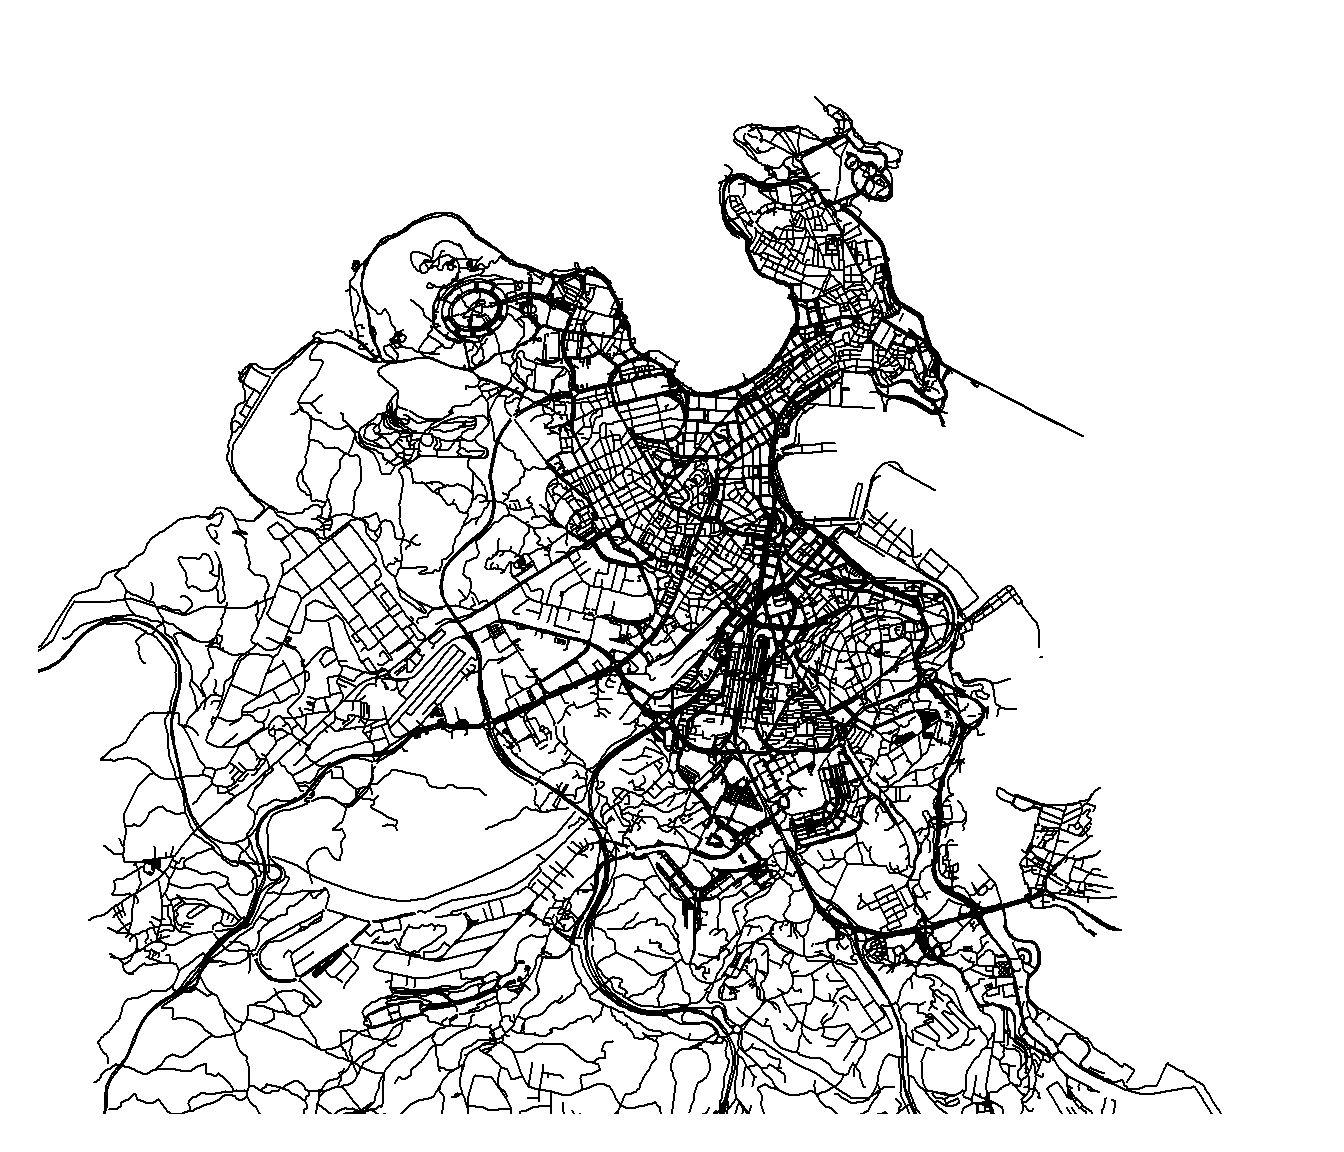
\includegraphics[width=0.7\linewidth]{images/osmdata-1} 

}

\caption{Representación de las carreteras, calles y caminos en A Coruña (generado con el paquete `osmdata`).}\label{fig:osmdata-plot}
\end{figure}

También están disponibles una gran cantidad de páginas web y geoportales desde donde es posible descargar datos espaciales (algo que se puede hacer directamente desde R).
Algunas de ellas son:

\begin{itemize}
\item
  \href{https://www.gadm.org}{CGADM database of Global Administrative Areas}: permite descargar límites administrativos a distintos niveles (e.g.~0 = pais, 1 = CCAA, 2 = provincias, 3 = comarcas, 4 = ayuntamientos).
\item
  \href{https://earthdata.nasa.gov}{NASA Earth Science Data}.
\item
  \href{https://inspire-geoportal.ec.europa.eu}{INSPIRE Geoportal}: \emph{Enhancing access to European spatial data}.
\item
  \href{https://scihub.copernicus.eu}{Copernicus Open Access Hub}: \emph{Europe's eyes on Earth}.
\end{itemize}

\hypertarget{operaciones-con-geometruxedas}{%
\subsection{Operaciones con geometrías}\label{operaciones-con-geometruxedas}}

Operaciones \href{https://r-spatial.github.io/sf/reference/geos_unary.html}{unarias} (operan sobre un único conjunto de geometrías simples, el primer argumento) con resultado geométrico:

\begin{itemize}
\tightlist
\item
  \texttt{st\_geometry()}: devuelve (o establece) la columna \texttt{sfc} de un objeto \texttt{sf}.
\item
  \texttt{st\_transform(x,\ crs,\ ...)}: transforma o convierte las coordenadas de \texttt{x} a un nuevo sistema de referencia.
\item
  \texttt{st\_cast(x,\ to,\ ...)}: cambia la geometría \texttt{x} a otro tipo de geometría.
\item
  \texttt{st\_centroid()}: devuelve los centroides de las geometrías.
\item
  \texttt{st\_buffer()}: crea un buffer en torno a la geometría o a cada geometría.
\item
  \texttt{st\_boundary()}: devuelve la frontera de la geometría.
\item
  \texttt{st\_convex\_hull()}: crea el envoltorio convexo de un conjunto de puntos.
\item
  \texttt{st\_voronoi()}: crea una \href{https://en.wikipedia.org/wiki/Voronoi_diagram}{teselación de Voronoi}.
\item
  \texttt{st\_make\_grid(x,\ cellsize,\ offset,\ n,\ what\ =\ c("polygons",\ "corners",\ "centers"))}: genera una rejilla rectangular (o exagonal) de geometrías (\texttt{what}) que cubre los límites de \texttt{x}.
\end{itemize}

Como ya se comentó en la Sección \ref{crs}, nos puede interesar transformar las coordenadas a un nuevo sistema de referencia (algo necesario para poder combinar conjuntos de datos espaciales con distintos CRS).
Por ejemplo podemos utilizar la \href{https://en.wikipedia.org/wiki/Mollweide_projection}{proyección de Mollweide} para representar datos globales (en este caso estimaciones de la población de países; Figura \ref{fig:transform} derecha).

\begin{Shaded}
\begin{Highlighting}[]
\FunctionTok{library}\NormalTok{(rnaturalearth) }
\NormalTok{par\_old }\OtherTok{\textless{}{-}} \FunctionTok{par}\NormalTok{(}\AttributeTok{mfrow =} \FunctionTok{c}\NormalTok{(}\DecValTok{1}\NormalTok{, }\DecValTok{2}\NormalTok{), }\AttributeTok{mar =} \FunctionTok{c}\NormalTok{(}\AttributeTok{bottom =} \DecValTok{0}\NormalTok{, }\AttributeTok{left =} \DecValTok{0}\NormalTok{, }\AttributeTok{top =} \DecValTok{0}\NormalTok{, }\AttributeTok{right =} \DecValTok{0}\NormalTok{))}
\CommentTok{\# NOTA: plot.sf() con escala no es compatible con mfrow }
\NormalTok{world\_pop }\OtherTok{\textless{}{-}} \FunctionTok{ne\_countries}\NormalTok{(}\AttributeTok{returnclass =} \StringTok{"sf"}\NormalTok{)[}\StringTok{"pop\_est"}\NormalTok{]}
\FunctionTok{plot}\NormalTok{(world\_pop, }\AttributeTok{logz =} \ConstantTok{TRUE}\NormalTok{, }\AttributeTok{main =} \StringTok{""}\NormalTok{, }\AttributeTok{key.pos =} \ConstantTok{NULL}\NormalTok{, }\AttributeTok{reset =} \ConstantTok{FALSE}\NormalTok{)}
\NormalTok{grat }\OtherTok{\textless{}{-}} \FunctionTok{st\_graticule}\NormalTok{(}\AttributeTok{crs=}\FunctionTok{st\_crs}\NormalTok{(}\StringTok{"WGS84"}\NormalTok{), }\AttributeTok{lon =} \FunctionTok{seq}\NormalTok{(}\SpecialCharTok{{-}}\DecValTok{180}\NormalTok{, }\DecValTok{180}\NormalTok{, }\AttributeTok{by =} \DecValTok{20}\NormalTok{), }\AttributeTok{lat =} \FunctionTok{seq}\NormalTok{(}\SpecialCharTok{{-}}\DecValTok{90}\NormalTok{, }\DecValTok{90}\NormalTok{, }\AttributeTok{by =} \DecValTok{10}\NormalTok{))}
\FunctionTok{plot}\NormalTok{(grat[}\DecValTok{1}\NormalTok{], }\AttributeTok{col =} \StringTok{\textquotesingle{}darkgray\textquotesingle{}}\NormalTok{, }\AttributeTok{add =} \ConstantTok{TRUE}\NormalTok{)}
\CommentTok{\# https://spatialreference.org/ref/esri/54009/}
\NormalTok{world\_pop2 }\OtherTok{\textless{}{-}} \FunctionTok{st\_transform}\NormalTok{(world\_pop, }\StringTok{"ESRI:54009"}\NormalTok{) }
\FunctionTok{plot}\NormalTok{(world\_pop2, }\AttributeTok{logz =} \ConstantTok{TRUE}\NormalTok{, }\AttributeTok{main =} \StringTok{""}\NormalTok{, }\AttributeTok{key.pos =} \ConstantTok{NULL}\NormalTok{, }\AttributeTok{reset =} \ConstantTok{FALSE}\NormalTok{)}
\NormalTok{grat }\OtherTok{\textless{}{-}} \FunctionTok{st\_graticule}\NormalTok{(world\_pop2, }\AttributeTok{lon =} \FunctionTok{seq}\NormalTok{(}\SpecialCharTok{{-}}\DecValTok{180}\NormalTok{, }\DecValTok{180}\NormalTok{, }\AttributeTok{by =} \DecValTok{20}\NormalTok{), }\AttributeTok{lat =} \FunctionTok{seq}\NormalTok{(}\SpecialCharTok{{-}}\DecValTok{90}\NormalTok{, }\DecValTok{90}\NormalTok{, }\AttributeTok{by =} \DecValTok{10}\NormalTok{))}
\FunctionTok{plot}\NormalTok{(grat[}\DecValTok{1}\NormalTok{], }\AttributeTok{col =} \StringTok{\textquotesingle{}darkgray\textquotesingle{}}\NormalTok{, }\AttributeTok{add =} \ConstantTok{TRUE}\NormalTok{)}
\end{Highlighting}
\end{Shaded}

\begin{figure}[!htb]

{\centering 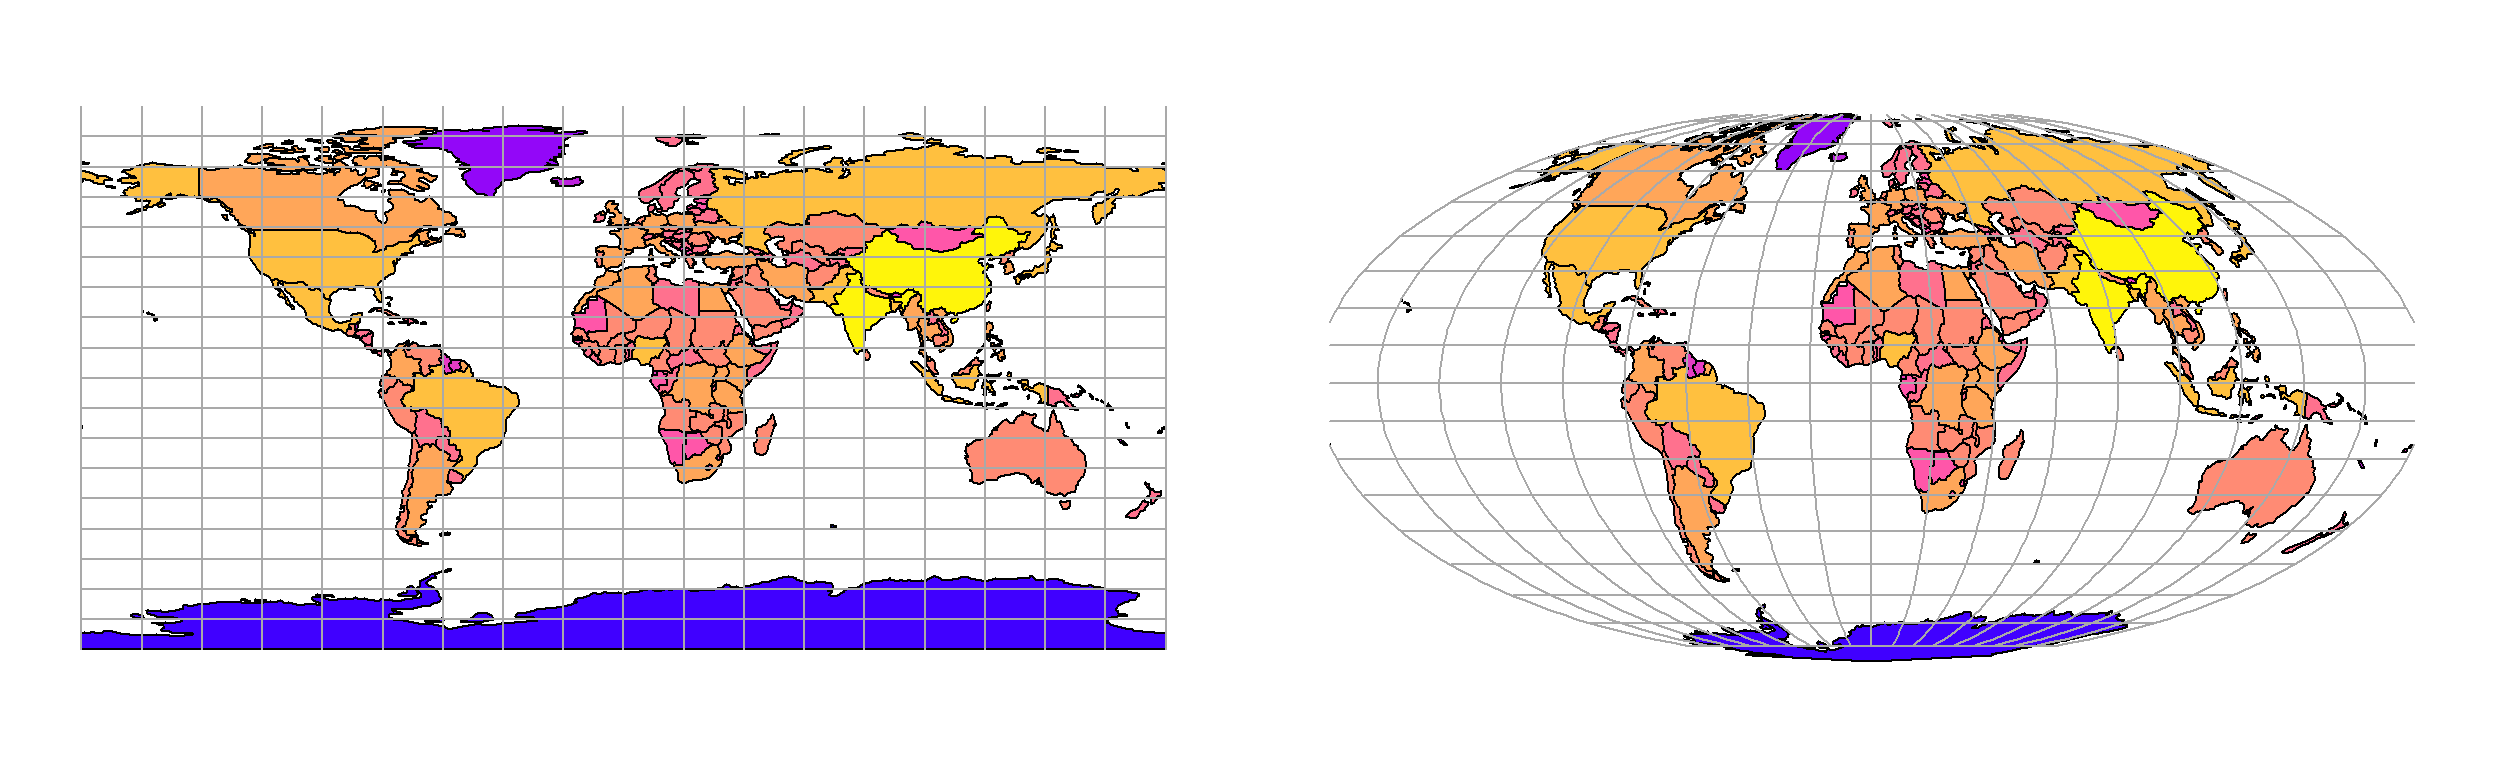
\includegraphics[width=1\linewidth]{02-datos_files/figure-latex/transform-1} 

}

\caption{Mapa de la población estimada por paises (en escala logarítmica), datos sin proyectar (izquierda) y con proyección de Mollweide (derecha).}\label{fig:transform}
\end{figure}

\begin{Shaded}
\begin{Highlighting}[]
\FunctionTok{par}\NormalTok{(par\_old)}
\end{Highlighting}
\end{Shaded}

Operaciones \href{https://r-spatial.github.io/sf/reference/geos_binary_ops.html}{binarias} (operan sobre dos conjuntos de geometrías simples) con resultado geométrico:

\begin{itemize}
\tightlist
\item
  \texttt{st\_union(x,\ y,\ ...,\ by\_feature)}: une varias geometrías.
\item
  \texttt{st\_intersection(x,\ y,\ ...)}: intersección de pares de geometrías.
\item
  \texttt{st\_crop(x,\ y,\ ...,\ xmin,\ ymin,\ xmax,\ ymax)}: intersección con rectángulo delimitador o especificado.
\item
  \texttt{st\_difference(x,\ y,\ ...)}: diferencia de pares de geometrías.
\item
  \texttt{st\_sym\_difference(x,\ y,\ ...)}: diferencia simétrica (xor) de pares de geometrías.
\item
  \texttt{st\_nearest\_points(x,\ y,\ ...)}: obtiene los puntos más cercanos entre pares de geometrías.
\end{itemize}

Operaciones unarias con resultado numérico o lógico:

\begin{itemize}
\tightlist
\item
  \texttt{st\_coordinates(x)}: devuelve una matriz con las coordenadas.
\item
  \texttt{st\_bbox(obj,\ ...)}: devuelve los límites del conjunto de geometrías.
\item
  \texttt{st\_area(x,\ ...)}: devuelve el área de polígonos.
\item
  \texttt{st\_length(x,\ ...)}: devuelve la longitud de líneas.
\item
  \texttt{st\_is(x,\ type)}: verifica si la geometría es de un determinado tipo o conjunto de clases.
\end{itemize}

Operaciones binarias con resultado numérico o \href{https://r-spatial.github.io/sf/reference/geos_binary_pred.html}{lógico}:

\begin{itemize}
\tightlist
\item
  \texttt{st\_distance(x,\ y,\ ...,\ by\_element,\ which)}: devuelve la matriz de distancias mínimas entre geometrías.
\item
  \texttt{st\_nearest\_feature(x,\ y)}: devuelve el índice de la geometría de \texttt{y} más cercana a cada geometría de \texttt{x}.
\item
  \texttt{st\_intersects(x,\ y,\ ...)}: determina si las geometrías se solapan o tocan.
\item
  \texttt{st\_disjoint(x,\ y,\ ...)}: determina si las geometrías no se solapan o tocan.
\item
  \texttt{st\_touches(x,\ y,\ ...)}: determina si las geometrías se tocan.
\item
  \texttt{st\_overlaps(x,\ y,\ ...)}: determina si las geometrías se solapan, pero no están completamente contenidas la una en la otra.
\item
  \texttt{st\_crosses(x,\ y,\ ...)}: determina si las geometrías se cruzan, pero no se tocan.
\item
  \texttt{st\_within(x,\ y,\ ...)}: determina si \texttt{x} está en \texttt{y}.
\item
  \texttt{st\_contains(x,\ y,\ ...)}: determina si \texttt{y} está en \texttt{x}.
\item
  \texttt{st\_covers(x,\ y,\ ...)}: determina si todos los puntos de \texttt{y} están dentro de \texttt{x}.
\item
  \texttt{st\_covered\_by(x,\ y,\ ...)}: determina si todos los puntos de \texttt{x} están dentro de \texttt{y}.
\item
  \texttt{st\_equals(x,\ y,\ ...)}: determina si \texttt{x} es geométricamente igual a \texttt{y}.
\item
  \texttt{st\_equals\_exact(x,\ y,\ par,\ ...)}: determina si \texttt{x} es igual a \texttt{y} con cierta tolerancia.
\end{itemize}

El resultado de las operaciones lógicas es una matriz dispersa (de clase \texttt{sgbp}, \emph{sparse geometry binary predicate}), que se puede convertir a una matriz densa con \texttt{as.matrix()}.

\hypertarget{sp-eda}{%
\section{Análisis exploratorio de datos espaciales}\label{sp-eda}}

Como se comentó en la Sección \ref{objetivos-esquema}, el primer paso para estimar las componentes del modelo, la tendencia \(\mu(\mathbf{s})\) y el semivariograma \(\gamma(\mathbf{h})\), es realizar un análisis exploratorio de los datos.

Normalmente comenzaremos por un análisis descriptivo de la respuesta.
Sería deseable que su distribución fuese aproximadamente simétrica (de forma que los métodos
basados en mínimos cuadrados sean adecuados).
Si además la distribución es aproximadamente normal (después de eliminar la tendencia) tendría sentido emplear métodos basados en
máxima verosimilitud (Sección \ref{ml-fit}).
Si su distribución es muy asimétrica se puede pensar en transformarla como punto de partida
(aunque podría cambiarse posteriormente dependiendo del modelo final para la tendencia).

\begin{Shaded}
\begin{Highlighting}[]
\FunctionTok{load}\NormalTok{(}\StringTok{"datos/aquifer.RData"}\NormalTok{)}
\FunctionTok{str}\NormalTok{(aquifer)}
\end{Highlighting}
\end{Shaded}

\begin{verbatim}
## 'data.frame':    85 obs. of  3 variables:
##  $ lon : num  42.78 -27.4 -1.16 -18.62 96.47 ...
##  $ lat : num  127.6 90.8 84.9 76.5 64.6 ...
##  $ head: num  1464 2553 2158 2455 1756 ...
\end{verbatim}

\begin{Shaded}
\begin{Highlighting}[]
\FunctionTok{library}\NormalTok{(sf)}
\NormalTok{aquifer\_sf }\OtherTok{\textless{}{-}} \FunctionTok{st\_as\_sf}\NormalTok{(aquifer, }\AttributeTok{coords =} \FunctionTok{c}\NormalTok{(}\StringTok{"lon"}\NormalTok{, }\StringTok{"lat"}\NormalTok{), }\AttributeTok{agr =} \StringTok{"constant"}\NormalTok{)}
\NormalTok{z }\OtherTok{\textless{}{-}}\NormalTok{ aquifer\_sf}\SpecialCharTok{$}\NormalTok{head}\SpecialCharTok{/}\DecValTok{100}
\FunctionTok{summary}\NormalTok{(z)}
\end{Highlighting}
\end{Shaded}

\begin{verbatim}
##    Min. 1st Qu.  Median    Mean 3rd Qu.    Max. 
##   10.24   15.48   17.97   20.02   25.40   35.71
\end{verbatim}

\begin{Shaded}
\begin{Highlighting}[]
\FunctionTok{hist}\NormalTok{(z, }\AttributeTok{xlab =} \StringTok{"piezometric{-}head"}\NormalTok{, }\AttributeTok{main =} \StringTok{""}\NormalTok{, }\AttributeTok{freq =} \ConstantTok{FALSE}\NormalTok{)}
\FunctionTok{lines}\NormalTok{(}\FunctionTok{density}\NormalTok{(z), }\AttributeTok{col =} \StringTok{\textquotesingle{}blue\textquotesingle{}}\NormalTok{)}
\end{Highlighting}
\end{Shaded}

\begin{figure}[!htb]

{\centering 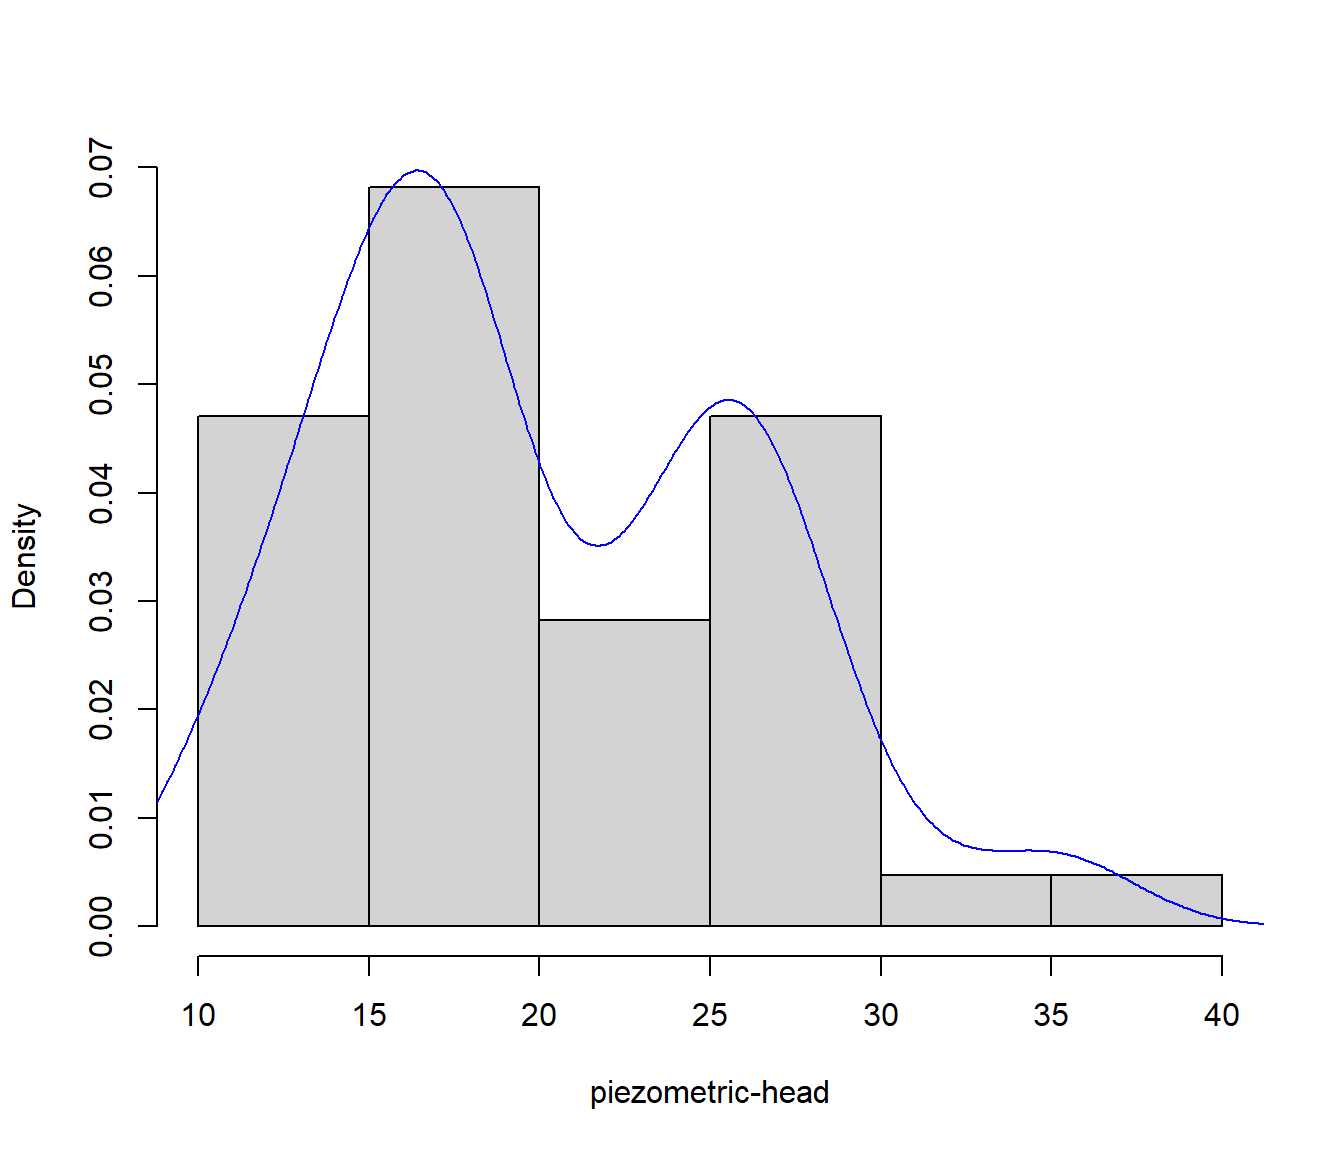
\includegraphics[width=0.7\linewidth]{02-datos_files/figure-latex/hist-aquifer-1} 

}

\caption{Distribución del nivel del agua subterránea en el acuífero Wolfcamp.}\label{fig:hist-aquifer}
\end{figure}

En un segundo paso se podría tener en cuenta las coordenadas espaciales.
Por ejemplo, podríamos generar un gráfico de dispersión para ver si se observa
algún patrón claro (lo que nos haría sospechar que la tendencia no es constante).

\begin{Shaded}
\begin{Highlighting}[]
\FunctionTok{plot}\NormalTok{(aquifer\_sf, }\AttributeTok{pch =} \DecValTok{20}\NormalTok{, }\AttributeTok{cex =} \DecValTok{3}\NormalTok{, }\AttributeTok{breaks =} \StringTok{"quantile"}\NormalTok{, }\AttributeTok{nbreaks =} \DecValTok{4}\NormalTok{)}
\end{Highlighting}
\end{Shaded}

\begin{figure}[!htb]

{\centering 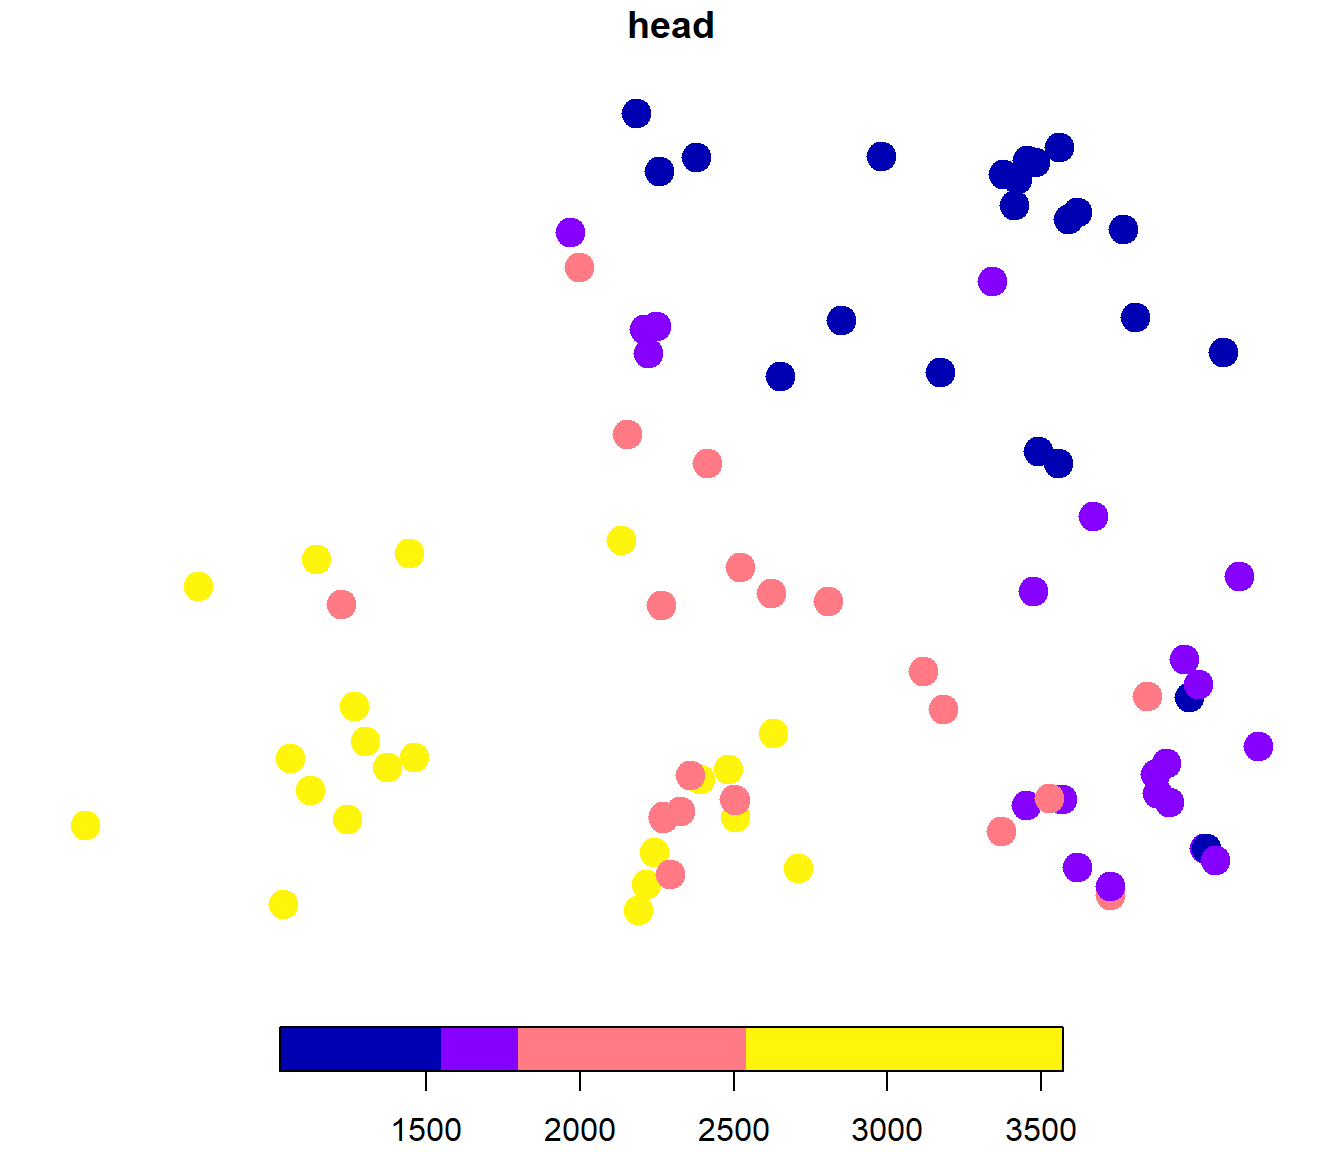
\includegraphics[width=0.7\linewidth]{02-datos_files/figure-latex/plot-aquifer-1} 

}

\caption{Distribución espacial de las observaciones del nivel del agua subterránea en el acuífero Wolfcamp.}\label{fig:plot-aquifer}
\end{figure}

Gráficos de dispersión de la respuesta frente a las coordenadas nos pueden ayudar a determinar si hay una tendencia (al estilo de las funciones \texttt{geoR::plot.geodata()} o \texttt{npsp::scattersplot()}):

\begin{Shaded}
\begin{Highlighting}[]
\NormalTok{coord }\OtherTok{\textless{}{-}} \FunctionTok{st\_coordinates}\NormalTok{(aquifer\_sf)}
\NormalTok{old.par }\OtherTok{\textless{}{-}} \FunctionTok{par}\NormalTok{(}\AttributeTok{mfrow =} \FunctionTok{c}\NormalTok{(}\DecValTok{1}\NormalTok{, }\DecValTok{2}\NormalTok{), }\AttributeTok{omd =} \FunctionTok{c}\NormalTok{(}\FloatTok{0.05}\NormalTok{, }\FloatTok{0.95}\NormalTok{, }\FloatTok{0.01}\NormalTok{, }\FloatTok{0.95}\NormalTok{))}
\FunctionTok{plot}\NormalTok{(coord[, }\DecValTok{1}\NormalTok{], z, }\AttributeTok{xlab =} \StringTok{"x"}\NormalTok{, }\AttributeTok{ylab =} \StringTok{"z"}\NormalTok{)}
\FunctionTok{lines}\NormalTok{(}\FunctionTok{lowess}\NormalTok{(coord[, }\DecValTok{1}\NormalTok{], z), }\AttributeTok{lty =} \DecValTok{2}\NormalTok{, }\AttributeTok{lwd =} \DecValTok{2}\NormalTok{, }\AttributeTok{col =} \StringTok{\textquotesingle{}blue\textquotesingle{}}\NormalTok{)}
\FunctionTok{plot}\NormalTok{(coord[, }\DecValTok{2}\NormalTok{], z, }\AttributeTok{xlab =} \StringTok{"y"}\NormalTok{, }\AttributeTok{ylab =} \StringTok{"z"}\NormalTok{)}
\FunctionTok{lines}\NormalTok{(}\FunctionTok{lowess}\NormalTok{(coord[, }\DecValTok{2}\NormalTok{], z), }\AttributeTok{lty =} \DecValTok{2}\NormalTok{, }\AttributeTok{lwd =} \DecValTok{2}\NormalTok{, }\AttributeTok{col =} \StringTok{\textquotesingle{}blue\textquotesingle{}}\NormalTok{)}
\end{Highlighting}
\end{Shaded}

\begin{figure}[!htb]

{\centering 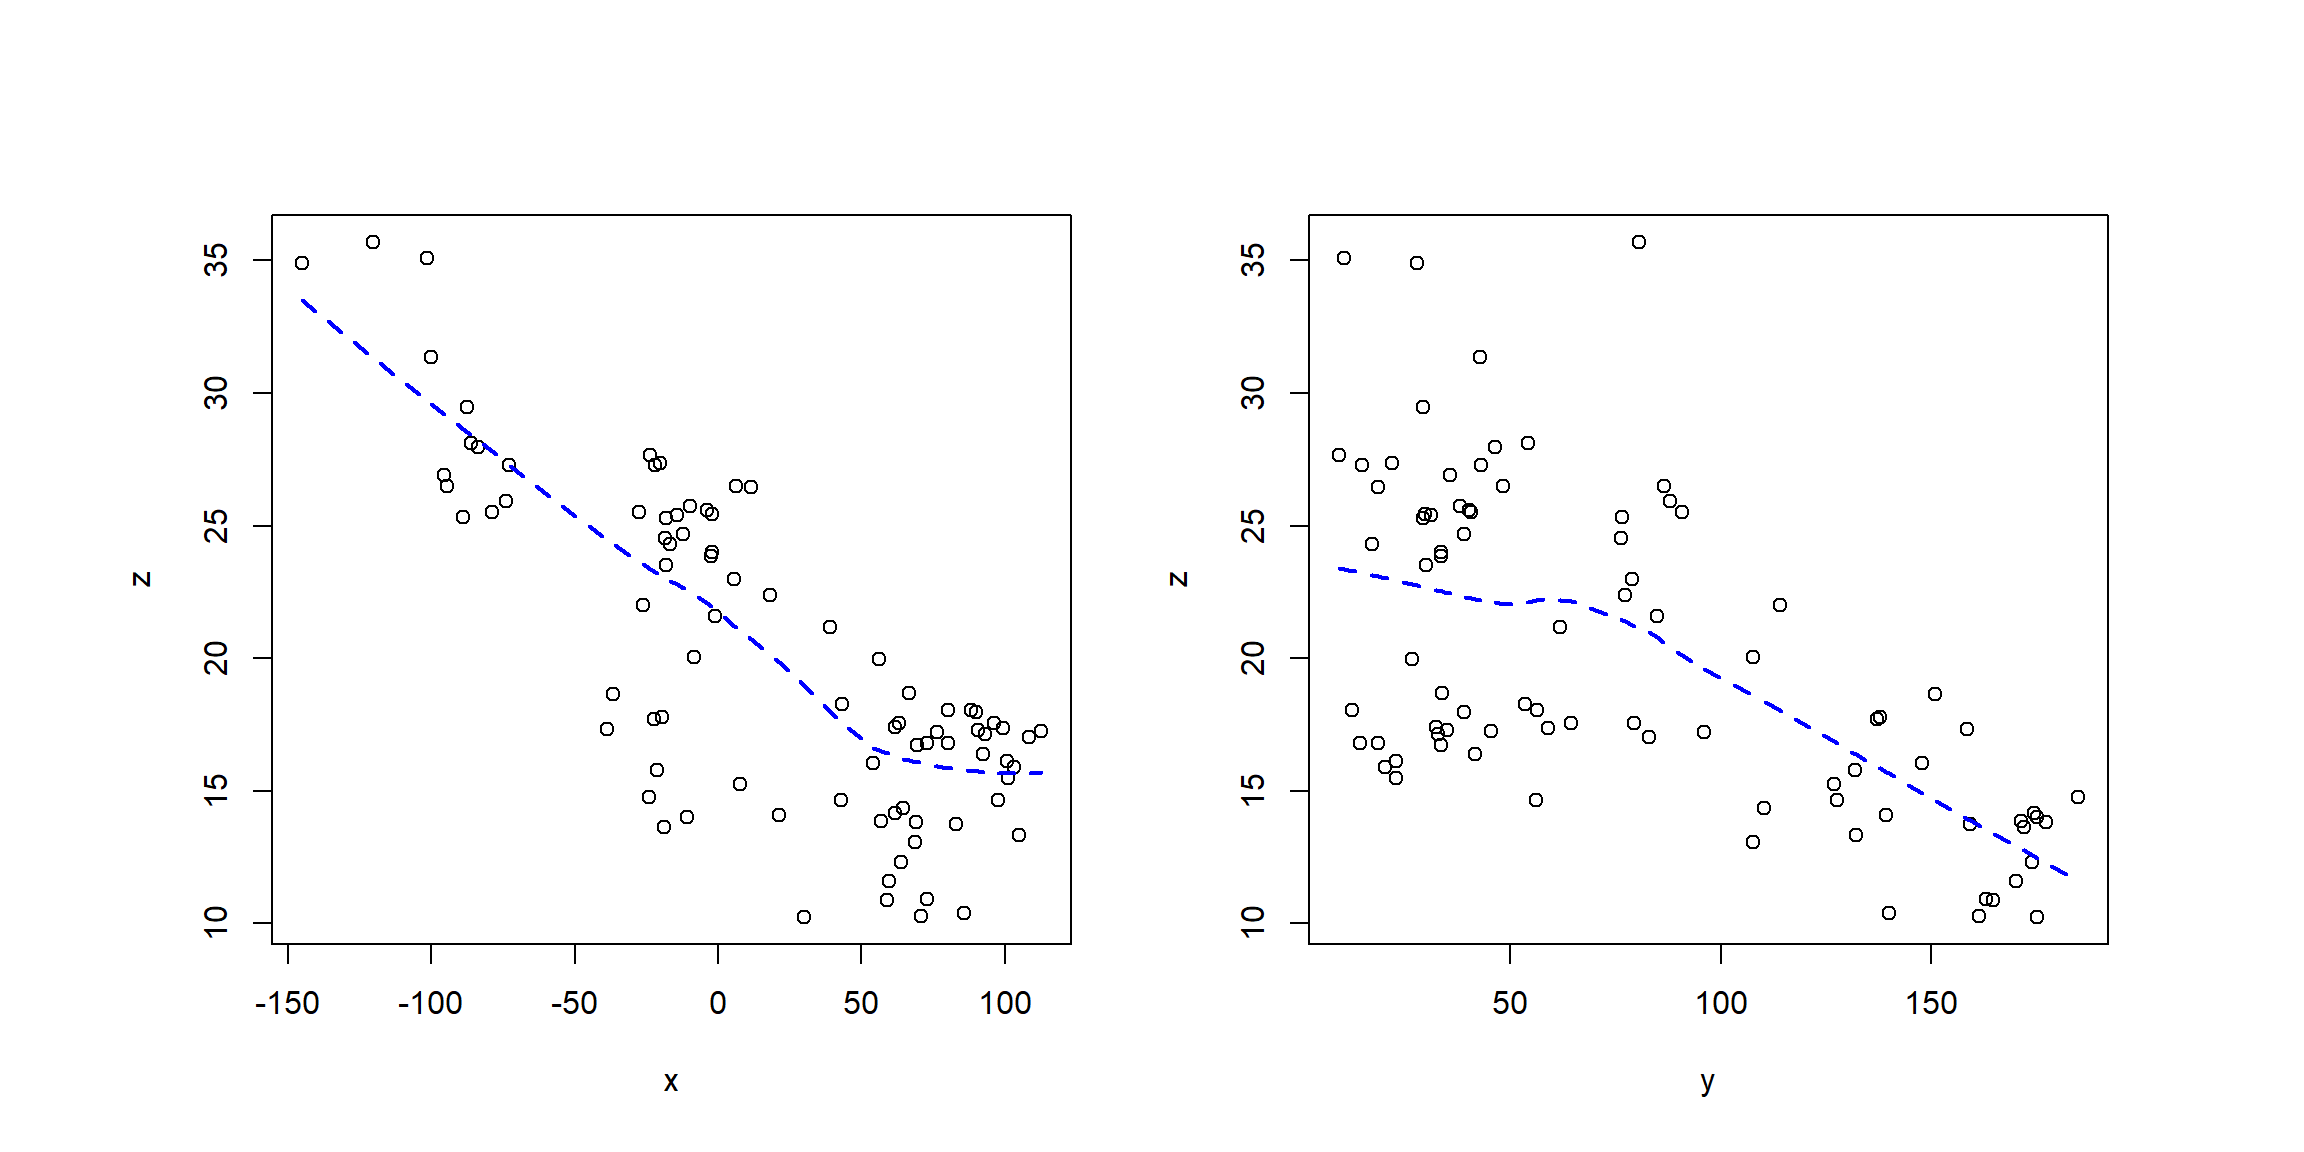
\includegraphics[width=0.9\linewidth]{02-datos_files/figure-latex/scattersplot-1} 

}

\caption{Gráficos de dispersión del nivel del agua subterránea frente a coordenadas (acuífero Wolfcamp).}\label{fig:scattersplot}
\end{figure}

\begin{Shaded}
\begin{Highlighting}[]
\FunctionTok{par}\NormalTok{(old.par)}
\end{Highlighting}
\end{Shaded}

En este caso concreto parece que una tendencia lineal es adecuada.

Para el análisis descriptivo de la dependencia se suelen emplear las semivarianzas o los estimadores experimentales del variograma, como se describe en la Sección \ref{vario-muestrales}.

\hypertarget{el-paquete-gstat}{%
\section{\texorpdfstring{El paquete \textbf{gstat}}{El paquete gstat}}\label{el-paquete-gstat}}

El paquete \href{https://r-spatial.github.io/gstat}{\texttt{gstat}} permite la modelización geoestadística (univariante, Capítulo 3, y multivariante, Capítulo 5), espacial y espacio-temporal (Capítulo 6), incluyendo predicción y simulación (Capítulo 4 y secciones 5.X y 6.X).

\begin{Shaded}
\begin{Highlighting}[]
\FunctionTok{library}\NormalTok{(gstat)}
\end{Highlighting}
\end{Shaded}

Este paquete implementa su propia estructura de datos (S3, basada en \texttt{data.frame}) pero también es compatible con los objetos \texttt{Spatial*} del paquete \texttt{sp} y los objetos de datos de los paquetes \texttt{sf} y \texttt{stars}.

Para más información se pueden consultar la \href{https://r-spatial.github.io/gstat/reference/index.html}{referencia}, las viñetas del paquete:

\begin{itemize}
\tightlist
\item
  \href{https://cran.r-project.org/web/packages/gstat/vignettes/gstat.pdf}{The meuse data set: a tutorial for the gstat R package},
\item
  \href{https://cran.r-project.org/web/packages/gstat/vignettes/spatio-temporal-kriging.pdf}{Spatio-Temporal Geostatistics using gstat},
\item
  \href{https://cran.r-project.org/web/packages/gstat/vignettes/st.pdf}{Introduction to Spatio-Temporal Variography},
\end{itemize}

el blog \href{https://r-spatial.org/}{r-spatial} o las correspondientes publicaciones (\href{http://www.sciencedirect.com/science/article/pii/S0098300404000676}{Pebesma, 2004}; \href{https://journal.r-project.org/archive/2016-1/na-pebesma-heuvelink.pdf}{Gräler, Pebesma y Heuvelink, 2016}).

Este paquete de R es una evolución de un programa independiente anterior con el mismo nombre (\href{http://www.sciencedirect.com/science/article/pii/S0098300497000824}{Pebesma y Wesseling, 1998}; basado en la librería \href{http://www.gslib.com}{GSLIB}, Deutsch y Journel, 1992).
Puede resultar de interés consultar el \href{http://www.gstat.org/gstat.pdf}{manual original} para información adicional sobre los detalles computacionales.

\hypertarget{modelado}{%
\chapter{Modelado de procesos geoestadísticos}\label{modelado}}

\textbf{\emph{En preparación\ldots{}}}

Como se comentó en la Sección \ref{objetivos-esquema} la aproximación tradicional (paramétrica) para el modelado de un proceso geoestadístico, es decir, estimar la tendencia \(\mu(\mathbf{s})\) y el semivariograma \(\gamma(\mathbf{h})\), consiste en los siguientes pasos:

\begin{enumerate}
\def\labelenumi{\arabic{enumi}.}
\item
  Análisis exploratorio y formulación de un modelo paramétrico (inicial).
\item
  Estimación de los parámetros del modelo:

  \begin{enumerate}
  \def\labelenumii{\arabic{enumii}.}
  \item
    Estimar y eliminar la tendencia (suponiendo que no es constante).
  \item
    Modelar la dependencia (ajustar un modelo de variograma) a partir de los residuos
    (o directamente de las observaciones si la tendencia se supone constante).
  \end{enumerate}
\item
  Validación del modelo o reformulación del mismo.
\item
  Empleo del modelo aceptado.
\end{enumerate}

El procedimiento habitual para el modelado de la dependencia en el paso 2 (también denominado \emph{análisis estructural}) consiste en obtener una estimación inicial del semivariograma utilizando algún tipo de estimador experimental (Sección \ref{vario-muestrales}) y posteriormente ajustar un modelo paramétrico válido de semivariograma a las estimaciones ``piloto'' obtenidas en el primer paso (secciones \ref{modelos-variog} y \ref{ajuste-variog}).

El principal problema con esta aproximación aparece cuando no se puede asumir que la tendencia es constante, ya que los estimadores muestrales descritos en la siguiente sección solo son adecuados para procesos estacionarios.
En este caso, como la media es constante, entonces:
\begin{equation} 
  E(Z(\mathbf{s}_1) - Z(\mathbf{s}_{2}))^2 = 2\gamma(\mathbf{s}_1 -\mathbf{s}_{2}),
  \ \forall \mathbf{s}_1 ,\mathbf{s}_{2} \in D.
\label{eq:vario-est}
\end{equation}
Sin embargo, cuando la tendencia no es constante:
\begin{equation} 
  E(Z(\mathbf{s}_1) - Z(\mathbf{s}_{2}))^2 = 2\gamma(\mathbf{s}_1 - \mathbf{s}_{2}) 
  + \left( \mu(\mathbf{s}_1)-\mu(\mathbf{s}_{2})\right)^2,
\label{eq:vario-nest}
\end{equation}
y no es necesariamente función de \(\mathbf{s}_1 -\mathbf{s}_{2}\), ni tiene por qué verificar las propiedades de un variograma.
Por este motivo, estos estimadores no deben ser utilizados mientras que no se elimine la tendencia de los datos.

Si no se puede asumir que la tendencia es constante, para poder estimarla de forma eficiente sería necesario conocer la dependencia (i.e.~conocer \(\gamma(\cdot)\)).
Este problema circular se suele resolver en la práctica realizando el paso 2 de forma iterativa, como se describe en la Sección 3.4.
Otra alternativa sería asumir normalidad y estimar ambos componentes de forma conjunta empleando alguno de los métodos basados en máxima verosimilitud descritos en la Sección \ref{ajuste-variog}.

Finalmente, en el paso 3, para verificar si el modelo (de tendencia y variograma) describe adecuadamente la variabilidad espacial de los datos (y para comparar modelos), se emplea normalmente la técnica de validación cruzada, descrita en la Sección 4.X del siguiente capítulo (en el que también se describe los principales métodos empleados en el paso 4).

\hypertarget{vario-muestrales}{%
\section{Estimadores muestrales del semivariograma}\label{vario-muestrales}}

Suponiendo que el proceso es intrísecamente estacionario, a partir de \eqref{eq:vario-est}, empleando el método de los momentos, se obtiene el denominado \emph{estimador empírico} (o clásico) del semivariograma (Matheron, 1962):
\[\hat{\gamma}(\mathbf{h}) = \dfrac{1}{2\left| N(\mathbf{h})\right| }
\sum\limits_{N(\mathbf{h})}\left( Z(\mathbf{s}_{i})-Z(\mathbf{s}_{j} )\right) ^2 ,\ \mathbf{h}\in \mathbb{R}^{d},\]
donde:
\[N(\mathbf{h}) = \left\{ (i,j):\mathbf{s}_{i} -\mathbf{s}_{j} \in Tol(\mathbf{h});i,j=1,\ldots,n\right\},\]
\(Tol(\mathbf{h})\subset \mathbb{R}^{d}\) es una región de tolerancia en torno a \(\mathbf{h}\) y \(\left| N(\mathbf{h})\right|\) es el número de pares distintos en \(N(\mathbf{h})\).
La región de tolerancia debería ser lo suficientemente grande como para que no aparezcan inestabilidades, por lo que se recomienda (Journel y Huijbregts 1978, p.194) que el numero de aportaciones a la estimación en un salto \(\mathbf{h}\) sea por lo menos de treinta (i.e.~\(\left| N(\mathbf{h})\right| \geq 30\)).

De forma análoga, suponiendo estacionariedad de segundo orden, se obtiene el estimador clásico del covariograma:
\[\hat{C} (\mathbf{h}) = \dfrac{1}{\left| N(\mathbf{h})\right| }
\sum\limits_{N(\mathbf{h})}\left( Z(\mathbf{s}_{i})-\bar{Z} \right)
\left( Z(\mathbf{s}_{j})-\bar{Z} \right),\ \mathbf{h}\in \mathbb{R}^{d},\]
siendo \(\bar{Z} =\frac{1}{n} \sum_{i=1}^{n}Z(\mathbf{s}_{i})\) la media muestral.
El principal problema con este estimador es la necesidad de estimar la media \(\mu\) del proceso, lo que produce que sea sesgado.
Por otra parte, además de que la suposición de estacionariedad de segundo orden es menos general (Sección \ref{procesos-estacionarios}, si el proceso es intrínsecamente estacionario el estimador del variograma es insesgado y también tiene mejores propiedades cuando la estimación se basa en residuos (aunque en este caso ambos estimadores son sesgados).
Más información sobre la distribución y propiedades de estos estimadores se tienen por ejemplo en Cressie (1993, pp.~71-74).
Estos resultados justifican que el modelado de la dependencia espacial se realice a través del semivariograma.

Uno de los problemas con el estimador empírico del semivariograma es su falta de robustez frente a observaciones atípicas.
Por este motivo se han propuesto numerosas alternativas robustas.
Hawkins y Cressie (1984) sugirieron promediar la raíz cuadrada de las diferencias en valor absoluto\footnote{Si el proceso \(Z(\cdot)\) es normal entonces
  \((Z(\mathbf{s})-Z(\mathbf{s}+\mathbf{h}))^2\) sigue una distribución \(2\gamma(\mathbf{h})\chi_1^2\), sin embargo esta distribución es muy asimétrica y la transformación de potencia que hace que se aproxime más a la simetría (normalidad) es la raíz cuarta. Otra ventaja de utilizar la raíz cuadrada de las diferencias es que, en general, están menos correladas que las diferencias al cuadrado (ver p.e. Cressie, 1993, p.~76).} y posteriormente transformar el resultado a la escala original tratando de obtener un estimador aproximadamente insesgado (utilizando del método delta), obteniéndose el estimador:

\[2\tilde{\gamma}(\mathbf{h}) = \left( \dfrac{1}{\left| N(\mathbf{h})\right| }
\sum\limits_{N(\mathbf{h})}\left| Z(\mathbf{s}_{i})-Z(\mathbf{s}_{j}
)\right|^{\frac{1}{2} } \right)^{4} /\left( \text{0.457+}
\dfrac{\text{0.494} }{\left| N(\mathbf{h})\right| } +\dfrac{\text{0.045}
}{\left| N(\mathbf{h})\right|^2 } \right).\]

Los estimadores locales tipo núcleo son herramientas frecuentemente utilizadas en la estimación de curvas y superficies.
Entre los más conocidos podemos señalar los estimadores tipo Nadaraya-Watson y los polinómicos locales (e.g.~Fan y Gijbels,1996).
Recientemente se han considerado también estas ideas para la estimación del covariograma (e.g.~Hall et al., 1994) y del semivariograma.
La expresión general de un estimador no paramétrico de un semivariograma isotrópico es de la forma:
\[\hat{\gamma}(r) = \dfrac{\sum\limits_{i=1}^{n-1}\sum\limits_{j=i+1}^{n}\omega_{ij}
(r)\left( Z(\mathbf{s}_{i})-Z(\mathbf{s}_{j})\right)^2  
}{2\sum\limits_{i=1}^{n-1}\sum\limits_{j=i+1}^{n}\omega_{ij}(r)},\]
donde \(\omega_{ij}(r) \geq 0\), \(\forall i,j\) y \(\sum_{i,j}\omega_{ij}(r) > 0\).
Dependiendo de la elección de estos pesos obtenemos distintos estimadores:

\begin{itemize}
\tightlist
\item
  \(\omega_{ij}(r) = \mathcal{I}_{Tol(r)} \left( \left\| \mathbf{s}_{i} - \mathbf{s}_{j} \right\| \right)\), siendo \(Tol(r)\subset \mathbb{R}\) una región de tolerancia en torno a \(r\) (y denotando por \(\mathcal{I}_{A}(\cdot)\) función indicadora del conjunto \(A\)), obtenemos el estimador clásico del semivariograma.
\item
  \(\omega_{ij}(r)=K\left( \frac{\left\| \mathbf{s}_{i} -\mathbf{s}_{j} \right\| -r}{h} \right)\), es el estimador Nadaraya-Watson (Hall et al., 1994).
\item
  \(\omega_{ij}(r)=K\left( \frac{\left\| \mathbf{s}_{i} -\mathbf{s}_{j} \right\| -r}{h} \right) \times\) \(\sum\limits_{k}\sum\limits_{l}K\left( \frac{\left\| \mathbf{s}_{k} -\mathbf{s}_{l} \right\| -r}{h} \right) \left( \left\| \mathbf{s}_{k} -\mathbf{s}_{l} \right\| -r\right) \left( \left\| \mathbf{s}_{k} -\mathbf{s}_{l} \right\| -\left\| \mathbf{s}_{i} -\mathbf{s}_{j} \right\| \right)\) se obtiene el estimador lineal local del semivariograma (García-Soidán et al., 2003).
\end{itemize}

La función \href{https://r-spatial.github.io/gstat/reference/variogram.html}{\texttt{variogram()}} del paquete \texttt{gstat}:

\begin{verbatim}
variogram(formula, locations = coordinates(data), data, cutoff, width = cutoff/15,
          cressie = FALSE, cloud = FALSE, covariogram = FALSE, ...)
\end{verbatim}

permite obtener la nube de semivarianzas (\texttt{cloud\ =\ TRUE}) y las estimaciones
empíricas o robustas (\texttt{cressie\ =\ TRUE}), además de otras posibilidades.

En primer lugar emplearemos el conjunto de datos \texttt{s100} del paquete \texttt{geoR}, que contiene una simulación de un proceso espacial estacionario (sin tendencia).

\begin{Shaded}
\begin{Highlighting}[]
\CommentTok{\# Cargamos los datos y los transformamos a un objeto \textasciigrave{}sf\textasciigrave{}}
\FunctionTok{library}\NormalTok{(sf)}
\end{Highlighting}
\end{Shaded}

\begin{verbatim}
## Linking to GEOS 3.9.1, GDAL 3.2.1, PROJ 7.2.1
\end{verbatim}

\begin{Shaded}
\begin{Highlighting}[]
\FunctionTok{data}\NormalTok{(s100, }\AttributeTok{package =} \StringTok{"geoR"}\NormalTok{)}
\NormalTok{datos }\OtherTok{\textless{}{-}} \FunctionTok{st\_as\_sf}\NormalTok{(}\FunctionTok{data.frame}\NormalTok{(s100}\SpecialCharTok{$}\NormalTok{coords, }\AttributeTok{z =}\NormalTok{ s100}\SpecialCharTok{$}\NormalTok{data), }
                  \AttributeTok{coords =} \DecValTok{1}\SpecialCharTok{:}\DecValTok{2}\NormalTok{, }\AttributeTok{agr =} \StringTok{"constant"}\NormalTok{)}
\end{Highlighting}
\end{Shaded}

\begin{Shaded}
\begin{Highlighting}[]
\FunctionTok{library}\NormalTok{(gstat)}
\NormalTok{vario.cloud }\OtherTok{\textless{}{-}} \FunctionTok{variogram}\NormalTok{(z }\SpecialCharTok{\textasciitilde{}} \DecValTok{1}\NormalTok{, datos, }\AttributeTok{cloud =} \ConstantTok{TRUE}\NormalTok{, }\AttributeTok{cutoff =} \FloatTok{0.6}\NormalTok{)}
\NormalTok{vario }\OtherTok{\textless{}{-}} \FunctionTok{variogram}\NormalTok{(z }\SpecialCharTok{\textasciitilde{}} \DecValTok{1}\NormalTok{, datos, }\AttributeTok{cloud =} \ConstantTok{FALSE}\NormalTok{, }\AttributeTok{cutoff =} \FloatTok{0.6}\NormalTok{)}
\CommentTok{\# Si se quiere tomar el 50\% del máximo salto (posible) cutoff = maxlag}
\CommentTok{\# maxlag \textless{}{-} 0.5*sqrt(sum(diff(apply(s100$coord, 2, range))\^{}2)) }
\CommentTok{\# maxlag \textless{}{-} 0.5*sqrt(sum(diff(matrix(st\_bbox(datos), nrow = 2, byrow = TRUE))\^{}2))}
\FunctionTok{names}\NormalTok{(vario)}
\end{Highlighting}
\end{Shaded}

\begin{verbatim}
## [1] "np"      "dist"    "gamma"   "dir.hor" "dir.ver" "id"
\end{verbatim}

NOTA: La componente \texttt{dist} contiene los saltos, \texttt{gamma} las estimaciones del semivariograma (semivarianzas) y \texttt{np} el número de aportaciones.

\begin{Shaded}
\begin{Highlighting}[]
\NormalTok{rvario.cloud }\OtherTok{\textless{}{-}} \FunctionTok{variogram}\NormalTok{(z }\SpecialCharTok{\textasciitilde{}} \DecValTok{1}\NormalTok{, datos, }\AttributeTok{cloud =} \ConstantTok{TRUE}\NormalTok{, }\AttributeTok{cressie =} \ConstantTok{TRUE}\NormalTok{, }\AttributeTok{cutoff =} \FloatTok{0.6}\NormalTok{)}
\NormalTok{rvario }\OtherTok{\textless{}{-}} \FunctionTok{variogram}\NormalTok{(z }\SpecialCharTok{\textasciitilde{}} \DecValTok{1}\NormalTok{, datos, }\AttributeTok{cloud =} \ConstantTok{FALSE}\NormalTok{, }\AttributeTok{cressie =} \ConstantTok{TRUE}\NormalTok{, }\AttributeTok{cutoff =} \FloatTok{0.6}\NormalTok{)}

\NormalTok{oldpar }\OtherTok{\textless{}{-}} \FunctionTok{par}\NormalTok{(}\AttributeTok{mfrow =} \FunctionTok{c}\NormalTok{(}\DecValTok{1}\NormalTok{, }\DecValTok{2}\NormalTok{))}
\FunctionTok{with}\NormalTok{(vario.cloud,  }\FunctionTok{plot}\NormalTok{(dist, gamma, }\AttributeTok{col =} \StringTok{"darkgray"}\NormalTok{, }
                        \AttributeTok{xlab =} \StringTok{"distance"}\NormalTok{, }\AttributeTok{ylab =}  \StringTok{"semivariance"}\NormalTok{))}
\FunctionTok{with}\NormalTok{(vario, }\FunctionTok{points}\NormalTok{(dist, gamma, }\AttributeTok{pch =} \DecValTok{19}\NormalTok{))}

\FunctionTok{with}\NormalTok{(rvario.cloud,  }\FunctionTok{plot}\NormalTok{(dist, gamma, }\AttributeTok{col =} \StringTok{"darkgray"}\NormalTok{, }
                        \AttributeTok{xlab =} \StringTok{"distance"}\NormalTok{, }\AttributeTok{ylab =}  \StringTok{"semivariance"}\NormalTok{))}
\FunctionTok{with}\NormalTok{(rvario, }\FunctionTok{points}\NormalTok{(dist, gamma, }\AttributeTok{pch =} \DecValTok{19}\NormalTok{))}
\end{Highlighting}
\end{Shaded}

\begin{center}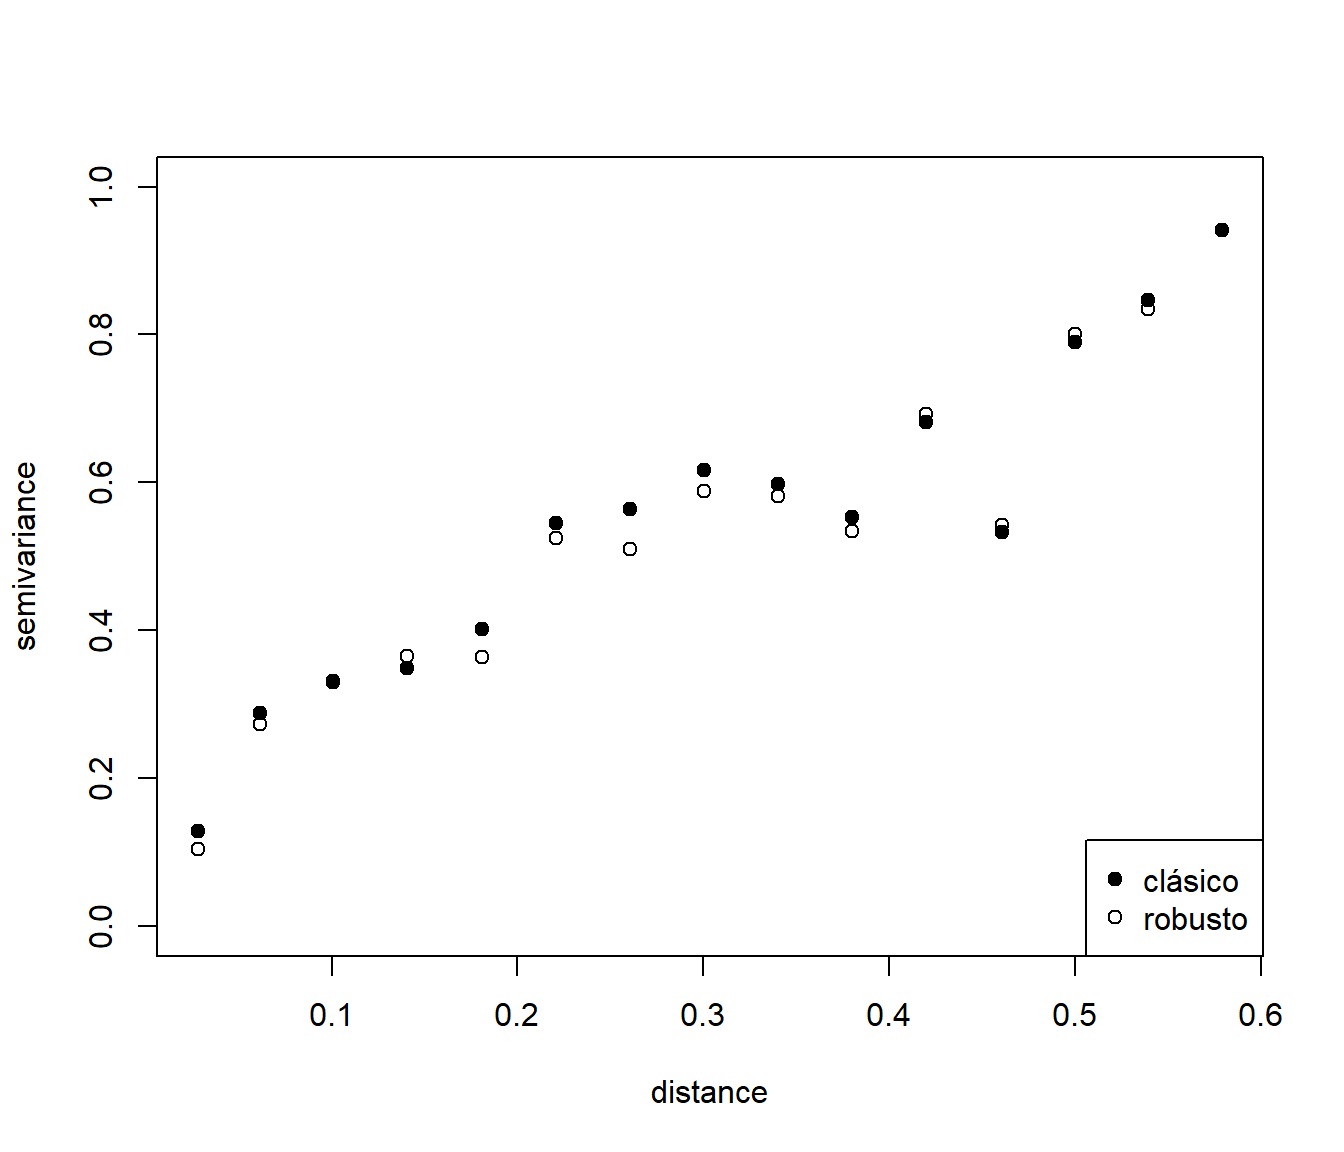
\includegraphics[width=0.9\linewidth]{03-modelado_files/figure-latex/vario-rvario-1} \end{center}

\begin{Shaded}
\begin{Highlighting}[]
\FunctionTok{par}\NormalTok{(oldpar)}
\end{Highlighting}
\end{Shaded}

Para un análisis exploratorio de la anisotropía, podemos obtener variogramas direccionales indicando el ángulo y los grados de tolerancia en cada eje:

\begin{Shaded}
\begin{Highlighting}[]
\FunctionTok{plot}\NormalTok{(}\FunctionTok{variogram}\NormalTok{(z }\SpecialCharTok{\textasciitilde{}} \DecValTok{1}\NormalTok{, datos, }\AttributeTok{cutoff =} \FloatTok{0.6}\NormalTok{, }\AttributeTok{alpha =} \FunctionTok{c}\NormalTok{(}\DecValTok{0}\NormalTok{, }\DecValTok{45}\NormalTok{, }\DecValTok{90}\NormalTok{, }\DecValTok{135}\NormalTok{)))}
\end{Highlighting}
\end{Shaded}

\begin{center}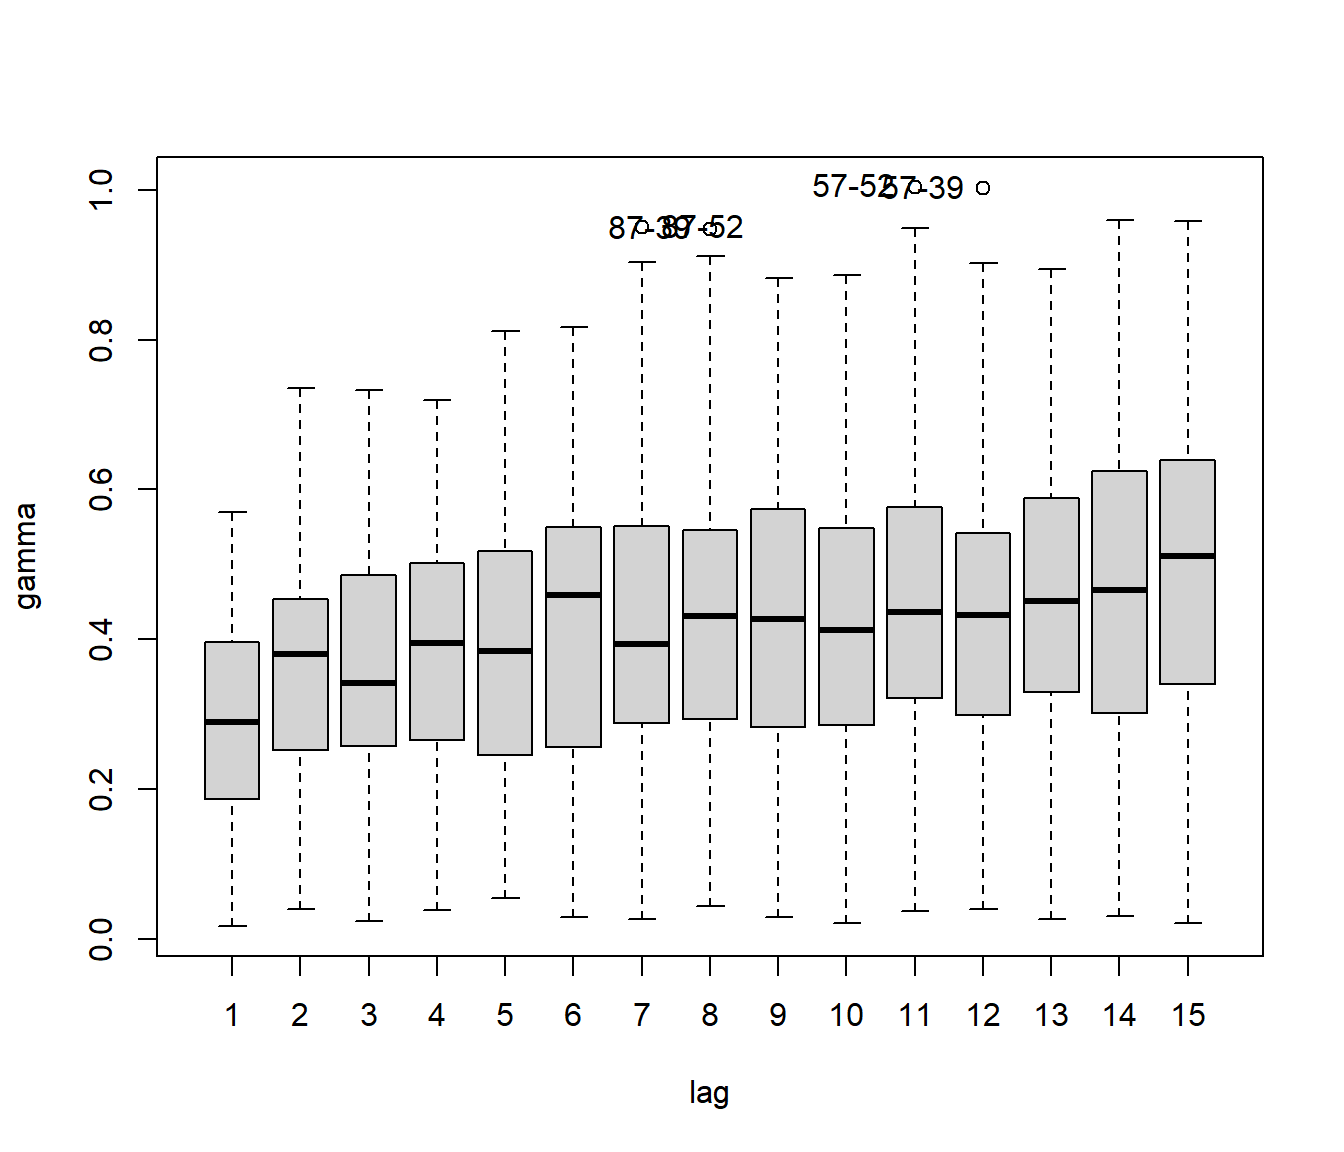
\includegraphics[width=0.7\linewidth]{03-modelado_files/figure-latex/unnamed-chunk-4-1} \end{center}

Complementariamente, se puede obtener un mapa de semivarianzas discretizadas en dos dimensiones:

\begin{Shaded}
\begin{Highlighting}[]
\NormalTok{variogram.map }\OtherTok{\textless{}{-}} \FunctionTok{variogram}\NormalTok{(z }\SpecialCharTok{\textasciitilde{}} \DecValTok{1}\NormalTok{, datos, }\AttributeTok{cutoff =} \FloatTok{0.6}\NormalTok{, }\AttributeTok{width =} \FloatTok{0.6} \SpecialCharTok{/} \DecValTok{15}\NormalTok{, }\AttributeTok{map =} \ConstantTok{TRUE}\NormalTok{)}
\FunctionTok{plot}\NormalTok{(variogram.map)}
\end{Highlighting}
\end{Shaded}

\begin{center}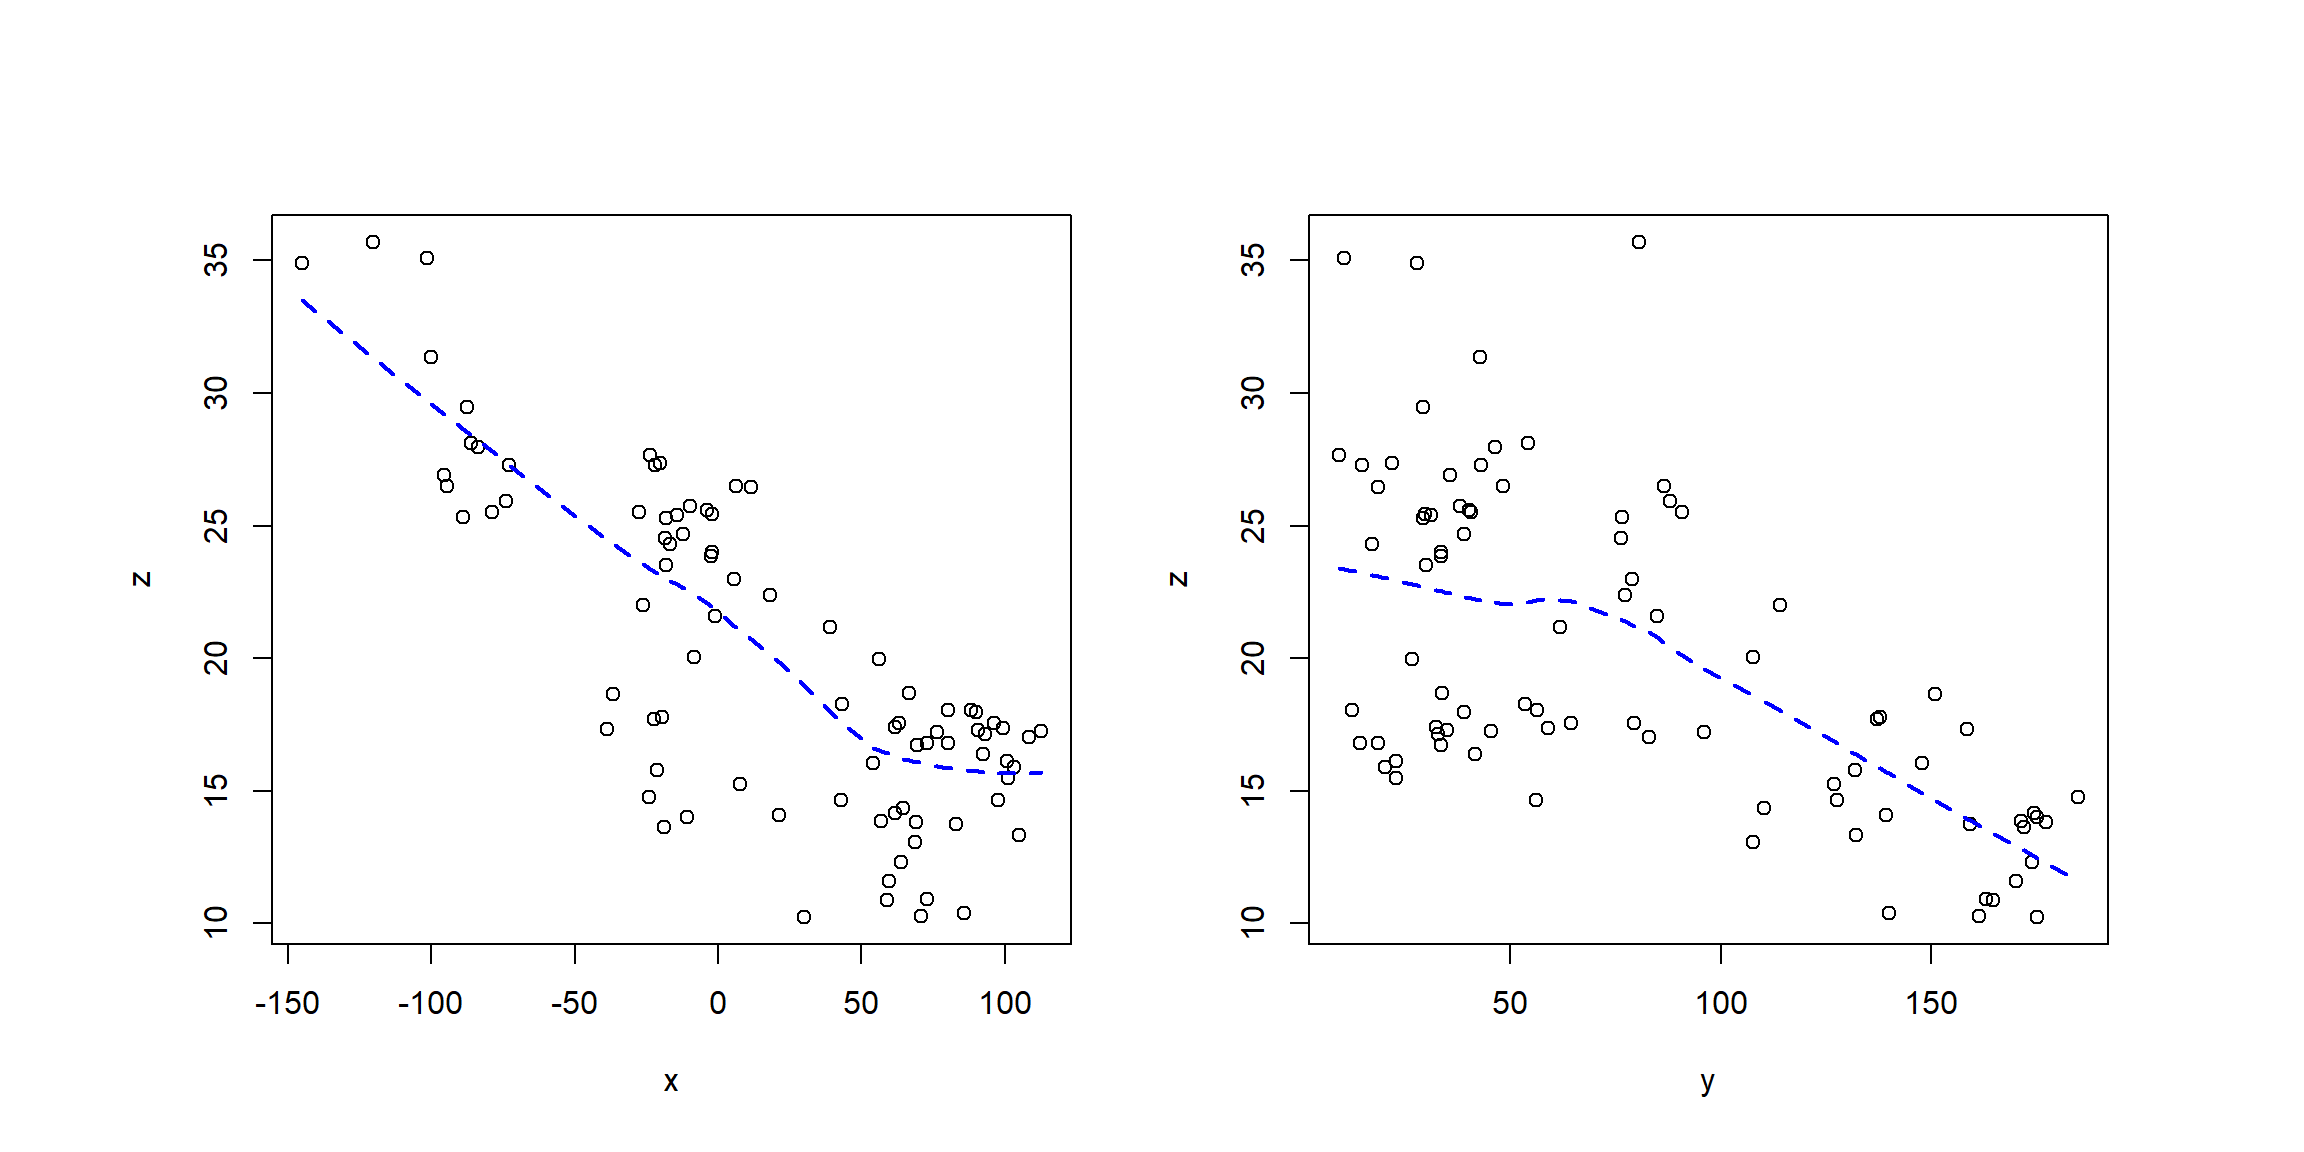
\includegraphics[width=0.7\linewidth]{03-modelado_files/figure-latex/unnamed-chunk-5-1} \end{center}

Para estudiar si hay dependencia espacial (estadísticamente significativa) se puede emplear la rutina \texttt{sm.variogram} del paquete \texttt{sm}.
Estableciendo \texttt{model\ =\ "independent"} devuelve un p-valor para contrastar la hipótesis nula de independencia
(i.e.~se acepta que hay una dependencia espacial si \(p \leq \alpha = 0.05\)) y un gráfico en el que se muestra el estimador empírico robusto, un estimador suavizado y una región de confianza para el variograma suponiendo que el proceso es independiente (i.e.~consideraríamos que hay dependencia espacial si el variograma suavizado no está contenido en esa región).

\begin{Shaded}
\begin{Highlighting}[]
\FunctionTok{library}\NormalTok{(sm)}
\end{Highlighting}
\end{Shaded}

\begin{verbatim}
## Package 'sm', version 2.2-5.7: type help(sm) for summary information
\end{verbatim}

\begin{Shaded}
\begin{Highlighting}[]
\FunctionTok{sm.variogram}\NormalTok{(s100}\SpecialCharTok{$}\NormalTok{coords, s100}\SpecialCharTok{$}\NormalTok{data, }\AttributeTok{model =} \StringTok{"independent"}\NormalTok{)}
\end{Highlighting}
\end{Shaded}

\begin{verbatim}
## Test of spatial independence: p =  0.024
\end{verbatim}

\begin{center}\includegraphics[width=0.7\linewidth]{03-modelado_files/figure-latex/unnamed-chunk-6-1} \end{center}

También se puede realizar contrastes adicionales estableciendo el parámetro \texttt{model} a \texttt{"isotropic"} o \texttt{"stationary"}.

\hypertarget{modelos-variog}{%
\section{Modelos de semivariogramas}\label{modelos-variog}}

Los variogramas deben ser condicionalmente semidefinidos negativos, una propiedad que los estimadores tradicionales normalmente no poseen.
Tradicionalmente esto se remedia ajustando un modelo paramétrico válido al estimador muestral (Sección \ref{ajuste-variog}).
En la Sección \ref{modelos-parametricos} se presentan algunos de los modelos isotrópicos tradicionalmente utilizados en geoestadística.
Estos modelos son empleados también en ciertos casos como estructuras básicas a partir de las cuales se construyen modelos más complejos, como modelos anisotrópicos (Sección \ref{anisotropia}) o los denominados modelos lineales de regionalización (Sección \ref{vario-lin-reg}).

\hypertarget{modelos-parametricos}{%
\subsection{Modelos paramétricos isotrópicos}\label{modelos-parametricos}}

A continuación se presentan algunos de los modelos isotrópicos de semivariograma más utilizados en geoestadística (una revisión más completa se tiene por ejemplo en Chilès y Delfiner, 1999, sección 2.5.1).
En la notación utilizada en las parametrizaciones \(c_{0} \geq 0\) representa el efecto nugget, \(c_1 \geq 0\) el umbral parcial (en el caso de variogramas acotados, con \(\sigma^2= c_0 + c_1\)) y \(a>0\) el rango (si existe) o el parámetro de escala.
En el caso de semivariogramas acotados que alcanzan el umbral asintóticamente (rango infinito), el parámetro \(a\) representa el rango práctico, definido como la distancia en la que el valor del semivariograma es el 95\% del umbral parcial.
En la Figura \ref{fig:show-vgms} se tienen algunos ejemplos de las formas de algunos de
estos semivariogramas.

\begin{itemize}
\item
  Modelo esférico:
  \[\gamma(\mathbf{h}\left| \boldsymbol{\theta}\right. ) = \left\{ 
  \begin{array}{ll}
  0 & \text{si} \left\| \mathbf{h}\right\| =0 \\
  c_{0} +c_1 \left\{ \dfrac{3}{2} \dfrac{\left\| \mathbf{h}\right\| }{a}
  -\dfrac{1}{2} \left( \dfrac{\left\| \mathbf{h}\right\| }{a} \right)
  3\right\}  & \text{si} 0<\left\| \mathbf{h}\right\| \leq a \\
  c_{0} +c_1  & \text{si} \left\| \mathbf{h}\right\| >a
  \end{array}
  \right.\]
  válido en \(\mathbb{R}^{d}\), \(d=1,2,3\).
\item
  Modelo exponencial:
  \[\gamma(\mathbf{h}\left| \boldsymbol{\theta}\right. )\ =\ \left\{ 
  \begin{array}{ll}
  0 & \text{si}\  \mathbf{h}=\mathbf{0} \\
  c_{0} + c_1 \left( 1-\exp \left( -\dfrac{3\left\|
  \mathbf{h}\right\| }{a} \right) \right)  & \text{si}\  \mathbf{h}\neq
  \mathbf{0}
  \end{array}
  \right.\]
  válido en \(\mathbb{R}^{d}\), \(\forall d \geq 1\).
\item
  Modelo racional cuadrático:
  \[\gamma(\mathbf{h}\left| \boldsymbol{\theta}\right. )\ =\ \left\{ 
  \begin{array}{ll}
  0 & \text{si}\  \mathbf{h}=\mathbf{0} \\
  c_{0} + c_1 \dfrac{\left\| \mathbf{h}\right\|^2
  }{\frac{1}{19} a^2 +\left\| \mathbf{h}\right\|^2 }  & \text{si}\ 
  \mathbf{h}\neq \mathbf{0}
  \end{array}
  \right.\]
  válido en \(\mathbb{R}^{d}\), \(\forall d \geq 1\).
\item
  Modelo potencial:
  \[\gamma(\mathbf{h}\left| \boldsymbol{\theta}\right. )\ =\ \left\{ 
  \begin{array}{ll}
  0 & \text{si}\  \mathbf{h}=\mathbf{0} \\
  c_{0} + a\left\| \mathbf{h}\right\|^{\lambda }  & \text{si}\ 
  \mathbf{h}\neq \mathbf{0}
  \end{array}
  \right.\]
  con \(0\leq \lambda <2\) y válido en \(\mathbb{R}^{d}\), \(\forall d \geq 1\).
  En el caso de \(\lambda =1\) se obtiene el conocido modelo lineal.
\item
  Modelo exponencial-potencial:
  \[\gamma(\mathbf{h}\left| \boldsymbol{\theta}\right. )\ =\ \left\{ 
  \begin{array}{ll}
  0 & \text{si}\  \mathbf{h}=\mathbf{0} \\
  c_{0} + c_1 \left( 1-\exp \left( -3\left( \dfrac{\left\|
  \mathbf{h}\right\| }{a} \right)^{\lambda } \right) \right)  & \text{si}\ 
  \mathbf{h}\neq \mathbf{0}
  \end{array}
  \right.\]
  con \(0\leq \lambda \leq 2\) y válido en \(\mathbb{R}^{d}\), \(\forall d \geq 1\).
  Cuando \(\lambda =2\) es denominado modelo gausiano;
  este modelo sin embargo no debería ser utilizado en la predicción
  espacial debido a las inestabilidades numéricas que produce en los
  algoritmos kriging (especialmente cuando el efecto nugget es grande; ver
  p.e. Wackernagel, 1998, pp.~120-123).
  El modelo exponencial se obtiene también como caso particular cuando \(\lambda =1\).
\item
  Modelo oscilatorio:
  \[\gamma(\mathbf{h}\left| \boldsymbol{\theta}\right. )\ =\ \left\{ 
  \begin{array}{ll}
  0 & \text{si}\  \mathbf{h}=\mathbf{0} \\
  c_{0} + c_1 \left( 1-\dfrac{a}{\left\| \mathbf{h}\right\| }
  \text{sen} \left( \dfrac{\left\| \mathbf{h}\right\| }{a} \right) \right) 
  & \text{si}\  \mathbf{h}\neq \mathbf{0}
  \end{array}
  \right.\]
  válido en \(\mathbb{R}^{d}\), \(d=1,2,3\).
  Este modelo con forma de onda (hay correlaciones negativas) alcanza su valor máximo ( \(c_{0} +1.218c_1\)) cuando \(\left\| \mathbf{h}\right\| \simeq 4.5a\), siendo \(a\) el parámetro de escala.
\item
  Modelo de Matérn (o K-Bessel):
  \[\gamma(\mathbf{h}\left| \boldsymbol{\theta}\right. )\ =\ \left\{ 
  \begin{array}{ll}
  0 & \text{si}\  \mathbf{h}=\mathbf{0} \\
  c_{0} + c_1 \left( 1-\dfrac{1}{2^{\nu -1} \gamma(\nu )} \left(
  \dfrac{\left\| \mathbf{h}\right\| }{a} \right)^{\nu } K_{\nu } \left(
  \dfrac{\left\| \mathbf{h}\right\| }{a} \right) \right)  & \text{si}\ 
  \mathbf{h}\neq \mathbf{0}
  \end{array}
  \right.\]
  siendo \(\nu \geq 0\) (un parámetro de suavizado) y \(K_{\nu }\) la función de Bessel modificada de tercera clase de orden \(\nu\) (ver p.e. Abramowitz y Stegun, 1965, pp.~374-379).
  Este modelo es válido en \(\mathbb{R}^{d}\), \(\forall d \geq 1\). El modelo exponencial se obtiene como caso particular cuando \(\nu =\frac{1}{2}\) y en el límite \(\nu \rightarrow \infty\) el modelo gausiano.
\end{itemize}

En \texttt{gstat} se emplea la función \texttt{vgm()} (\emph{Variogram Model}) para definir un modelo de variograma:

\begin{Shaded}
\begin{Highlighting}[]
\FunctionTok{vgm}\NormalTok{(}\AttributeTok{psill =} \ConstantTok{NA}\NormalTok{, model, }\AttributeTok{range =} \ConstantTok{NA}\NormalTok{, nugget, add.to, anis, }\AttributeTok{kappa =} \FloatTok{0.5}\NormalTok{, ...)}
\end{Highlighting}
\end{Shaded}

\begin{itemize}
\tightlist
\item
  \texttt{psill}: umbral parcial (\(c_1\)).
\item
  \texttt{model}: cadena de texto que identifica el modelo (e.g.~\texttt{"Exp"}, \texttt{"Sph"}, \texttt{"Gau"}, \texttt{"Mat"}\ldots).
\item
  \texttt{range}: rango o parámetro de escala (proporcional a \(a\)).
\item
  \texttt{nugget}: efecto nugget (\(c_0\)).
\item
  \texttt{kappa}: parametro de suavizado (\(\nu\) en el modelo de Matérn).
\item
  \texttt{add.to}: permite combinar modelos (Sección \ref{vario-lin-reg}).
\item
  \texttt{anis}: parámetros de anisotropía (Sección \ref{anisotropia}).
\end{itemize}

Lo habitual es definir un modelo para posteriormente estimar sus parámetros utilizando los empleados en la definición como valores iniciales. También se puede llamar a esta función con el modelo como primer y único argumento, indicando que los parámetros son desconocidos (o que tome los valores por defecto en el ajuste).
Si se ejecuta sin argumentos devuelve un listado de todos los modelos:

\begin{Shaded}
\begin{Highlighting}[]
\FunctionTok{vgm}\NormalTok{()}
\end{Highlighting}
\end{Shaded}

\begin{verbatim}
##    short                                      long
## 1    Nug                              Nug (nugget)
## 2    Exp                         Exp (exponential)
## 3    Sph                           Sph (spherical)
## 4    Gau                            Gau (gaussian)
## 5    Exc        Exclass (Exponential class/stable)
## 6    Mat                              Mat (Matern)
## 7    Ste Mat (Matern, M. Stein's parameterization)
## 8    Cir                            Cir (circular)
## 9    Lin                              Lin (linear)
## 10   Bes                              Bes (bessel)
## 11   Pen                      Pen (pentaspherical)
## 12   Per                            Per (periodic)
## 13   Wav                                Wav (wave)
## 14   Hol                                Hol (hole)
## 15   Log                         Log (logarithmic)
## 16   Pow                               Pow (power)
## 17   Spl                              Spl (spline)
## 18   Leg                            Leg (Legendre)
## 19   Err                   Err (Measurement error)
## 20   Int                           Int (Intercept)
\end{verbatim}

La función \texttt{show.vgms()} genera gráficos con los distintos modelos (por defecto los 17 primeros):

\begin{Shaded}
\begin{Highlighting}[]
\FunctionTok{show.vgms}\NormalTok{()}
\end{Highlighting}
\end{Shaded}

\begin{figure}[!htb]

{\centering 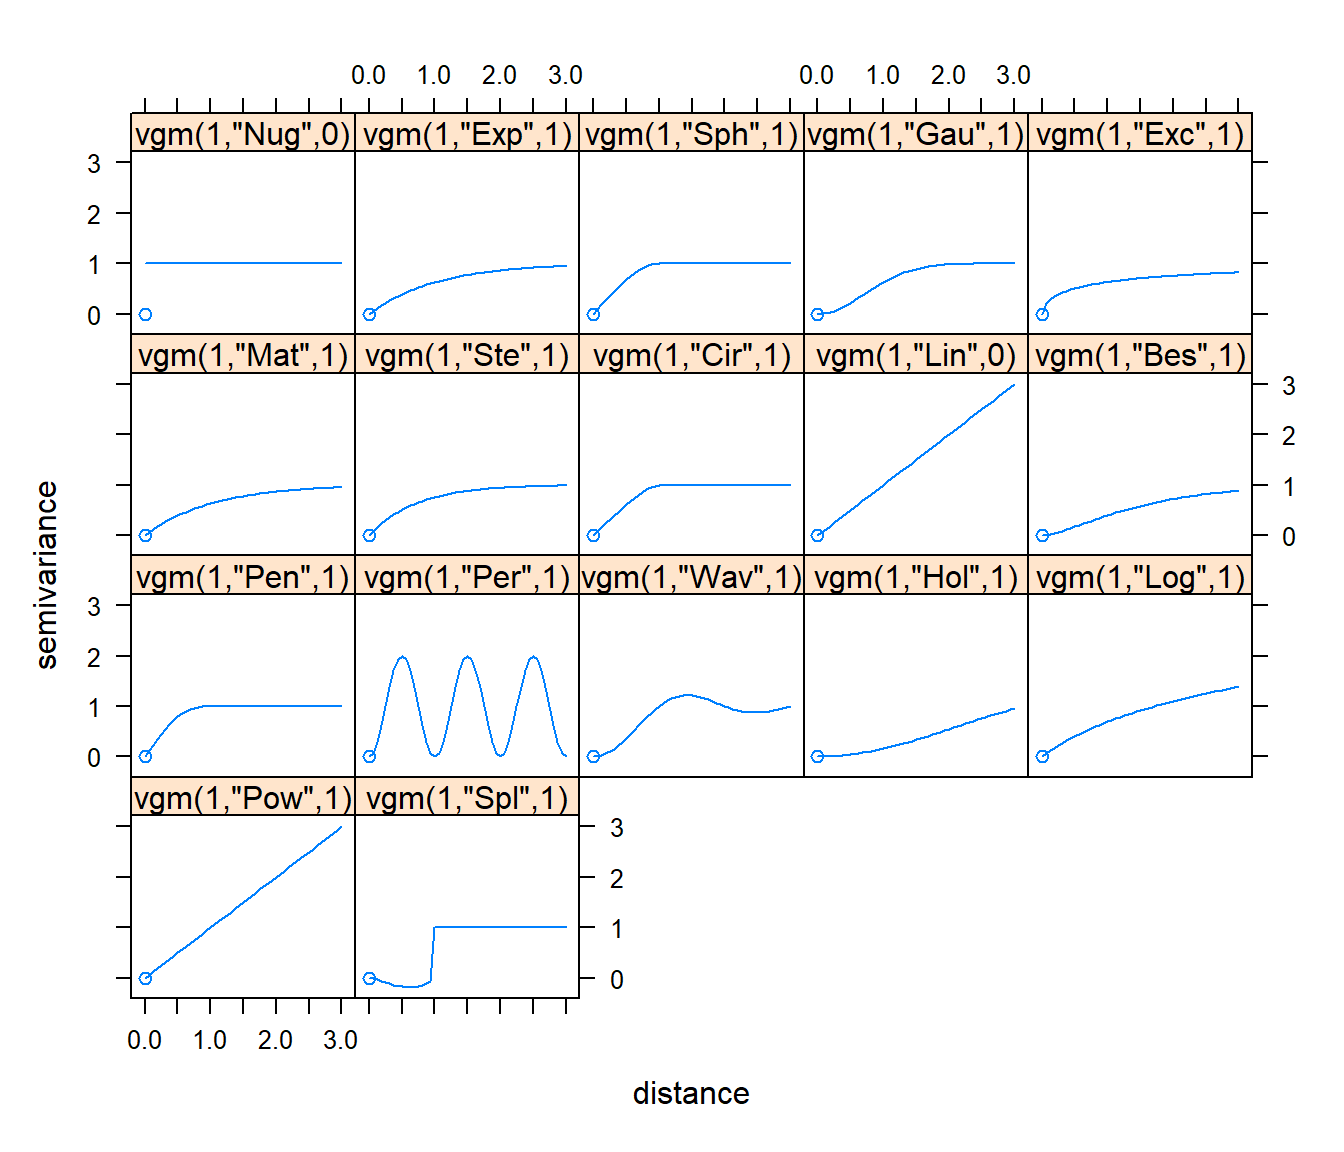
\includegraphics[width=0.7\linewidth]{03-modelado_files/figure-latex/show-vgms-1} 

}

\caption{Representaciones de los modelos paramétricos isotrópicos de semivariogramas implementados en el paquete `gstat`.}\label{fig:show-vgms}
\end{figure}

\begin{Shaded}
\begin{Highlighting}[]
\FunctionTok{show.vgms}\NormalTok{(}\AttributeTok{kappa.range =} \FunctionTok{c}\NormalTok{(}\FloatTok{0.1}\NormalTok{, }\FloatTok{0.5}\NormalTok{, }\DecValTok{1}\NormalTok{, }\DecValTok{5}\NormalTok{, }\DecValTok{10}\NormalTok{), }\AttributeTok{max =} \DecValTok{10}\NormalTok{)}
\end{Highlighting}
\end{Shaded}

\begin{figure}[!htb]

{\centering 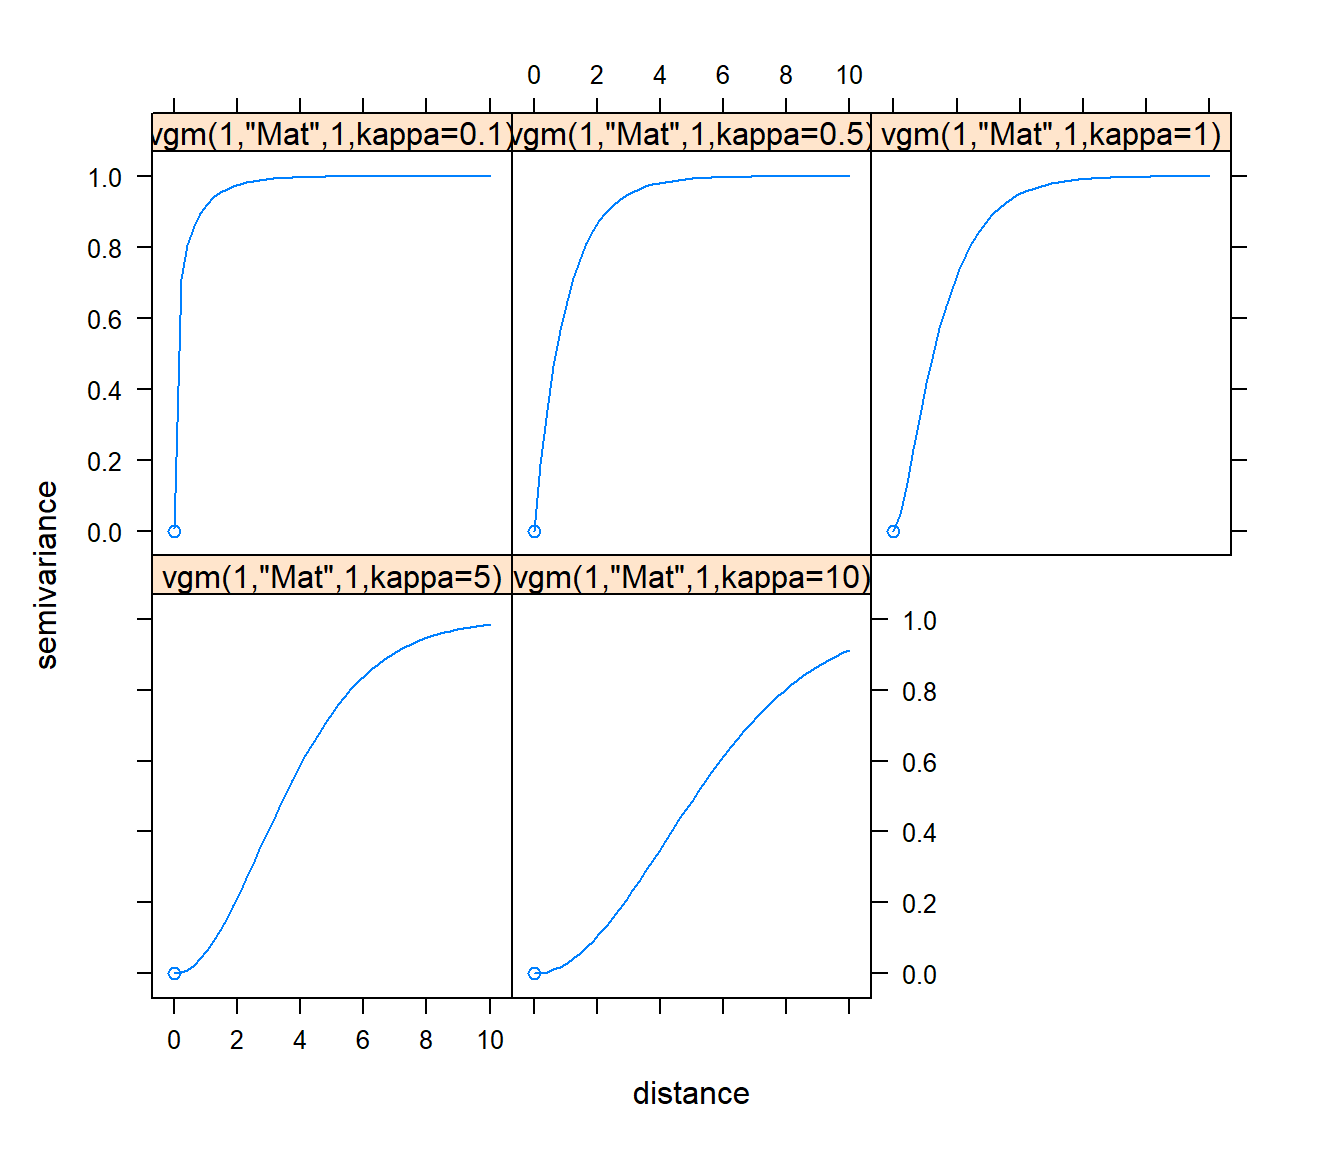
\includegraphics[width=0.7\linewidth]{03-modelado_files/figure-latex/show-matern-1} 

}

\caption{Modelo de Matérn con distintos valores del parámetro de suavizado.}\label{fig:show-matern}
\end{figure}

\begin{Shaded}
\begin{Highlighting}[]
\NormalTok{v1 }\OtherTok{\textless{}{-}} \FunctionTok{vgm}\NormalTok{(}\AttributeTok{psill =} \DecValTok{1}\NormalTok{, }\AttributeTok{model =} \StringTok{"Exp"}\NormalTok{, }\AttributeTok{range =} \FloatTok{0.5}\NormalTok{, }\AttributeTok{nugget =} \DecValTok{0}\NormalTok{)}
\NormalTok{v1}
\end{Highlighting}
\end{Shaded}

\begin{verbatim}
##   model psill range
## 1   Nug     0   0.0
## 2   Exp     1   0.5
\end{verbatim}

\begin{Shaded}
\begin{Highlighting}[]
\FunctionTok{plot}\NormalTok{(v1, }\AttributeTok{cutoff =} \DecValTok{3}\NormalTok{)}
\end{Highlighting}
\end{Shaded}

\begin{figure}[!htb]

{\centering 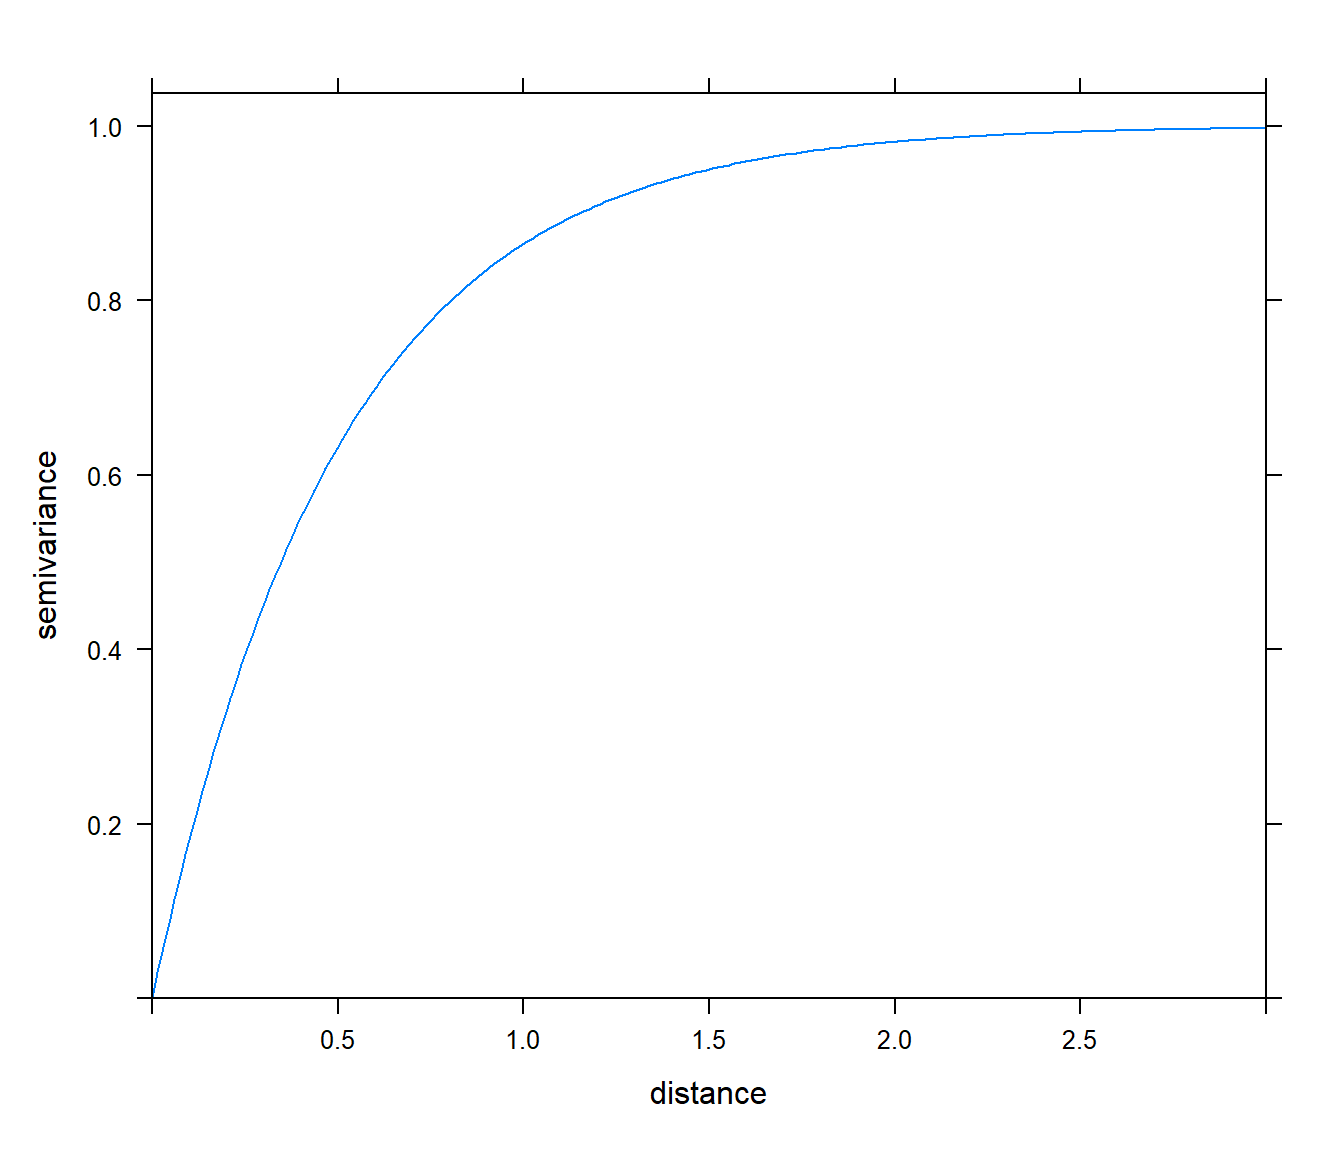
\includegraphics[width=0.7\linewidth]{03-modelado_files/figure-latex/vgm-exp-1} 

}

\caption{Ejemplo de modelo exponencial.}\label{fig:vgm-exp}
\end{figure}

\hypertarget{anisotropia}{%
\subsection{Modelado de anisotropía}\label{anisotropia}}

La hipótesis de isotropía simplifica notablemente el modelado de la dependencia espacial por lo que la mayoría de los modelos (básicos) de semivariogramas considerados en geoestadística son isotrópicos (Sección XX).
Sin embargo, en muchos casos no se puede asumir que la dependencia es igual en cualquier dirección (uno de los ejemplos más claros es el caso espacio-temporal, donde en principio no es razonable pensar que un salto espacial es equivalente a un salto temporal).
En esos casos se suelen considerar ligeras variaciones de la hipótesis de isotropía para modelar la dependencia espacial.
En esta sección se comentan brevemente las distintas aproximaciones tradicionalmente consideradas en geoestadística (para más detalles ver p.e. Chilès y Delfiner, 1999, sección 2.5.2, o Goovaerts, 1997, sección 4.2.2), otras aproximaciones adicionales se tratarán en el Capítulo 7 (caso espacio-temporal).

Cuando el variograma es función de la dirección además de la magnitud del salto, se dice que el variograma es anisotrópico (no isotrópico).
Los tipos de anisotropía habitualmente considerados son:

\begin{itemize}
\tightlist
\item
  \emph{Anisotropía geométrica}: cuando el umbral permanece constante mientras que el rango varía con la dirección.
\item
  \emph{Anisotropía zonal}: cuando el umbral del semivariograma varía con la dirección (también se denomina anisotropía estratificada).
\item
  Combinación de las anteriores.
\end{itemize}

La anisotropía geométrica se puede corregir mediante una transformación lineal del vector de salto \(\mathbf{h}\):
\[\gamma(\mathbf{h})=\gamma ^{0} \left( \left\| \mathbf{A}\mathbf{h}\right\| \right) ,\forall \mathbf{h}\in \mathbb{R}^{d},\]
siendo \(\mathbf{A}\) una matriz cuadrada \(d\times d\) y \(\gamma ^{0} (\cdot)\) un semivariograma isotrópico\footnote{Esta idea (que el espacio euclídeo no es apropiado para medir distancias entre posiciones espaciales pero una transformación lineal de él sí) ha sido también generalizada para el caso de deformaciones no lineales del espacio. Por ejemplo, Sampson y Guttorp (1992) consideraron transformaciones no lineales obtenidas mediante técnicas de escalamiento óptimo multidimensional.}.
En este caso se dice que el variograma es \emph{geométricamente anisotrópico}.
Por ejemplo, en el caso bidimensional, se suelen considerar una matriz de la forma:
\[\mathbf{A}=\left( 
\begin{array}{cc}
1  & 0 \\
0 & a_2/a_1 
\end{array}
\right) \left( 
\begin{array}{cc}
\cos \theta  & \sin\theta  \\
\text{-} \sin\theta  & \cos \theta 
\end{array}
\right),\]
que se corresponde con las direcciones principales de anisotropía \(\theta\) y \(\theta + \frac{\pi }{\text{2}}\) (normalmente se toma \(\theta\) igual a la dirección de máximo rango).
Esto puede extenderse fácilmente para el caso tridimensional (ver p.e. Chilès y Delfiner, 1999, pp.~94-95).

En \texttt{gstat} se puede definir anisotropía mediante el argumento \texttt{anis} de la función \texttt{vgm()}.
En dos dimensiones es un vector con dos componentes \texttt{aniso\ =\ c(alpha,\ ratio)}, \texttt{alpha} es el ángulo para la dirección principal de variabilidad (medido en el sentido del reloj partiendo de la dirección norte) y \texttt{ratio} la relación entre el rango mínimo y máximo (\(0 \leq ratio \leq 1\)).

Ejemplo:

\begin{Shaded}
\begin{Highlighting}[]
\NormalTok{v }\OtherTok{\textless{}{-}} \FunctionTok{vgm}\NormalTok{(}\DecValTok{1}\NormalTok{, }\StringTok{"Exp"}\NormalTok{, }\DecValTok{5}\NormalTok{, }\AttributeTok{anis =} \FunctionTok{c}\NormalTok{(}\DecValTok{30}\NormalTok{, }\FloatTok{0.1}\NormalTok{))}
\FunctionTok{str}\NormalTok{(v)}
\end{Highlighting}
\end{Shaded}

\begin{verbatim}
## Classes 'variogramModel' and 'data.frame':   1 obs. of  9 variables:
##  $ model: Factor w/ 20 levels "Nug","Exp","Sph",..: 2
##  $ psill: num 1
##  $ range: num 5
##  $ kappa: num 0.5
##  $ ang1 : num 30
##  $ ang2 : num 0
##  $ ang3 : num 0
##  $ anis1: num 0.1
##  $ anis2: num 1
\end{verbatim}

\begin{Shaded}
\begin{Highlighting}[]
\NormalTok{plot\_ellipse\_2d }\OtherTok{\textless{}{-}} \ControlFlowTok{function}\NormalTok{(}\AttributeTok{xc =} \DecValTok{0}\NormalTok{, }\AttributeTok{yc =} \DecValTok{0}\NormalTok{, }\AttributeTok{l1 =} \DecValTok{10}\NormalTok{, }\AttributeTok{l2 =} \DecValTok{1}\NormalTok{, }\AttributeTok{phi =}\NormalTok{ pi}\SpecialCharTok{/}\DecValTok{3}\NormalTok{, }
                            \AttributeTok{by =} \FloatTok{0.01}\NormalTok{, }\AttributeTok{asp =} \DecValTok{1}\NormalTok{, ...) \{}
    \CommentTok{\# xc, yc: centro}
    \CommentTok{\# l1, l2: longitud ejes}
    \CommentTok{\# phi: angulo del eje 1 respecto al eje x}
\NormalTok{    t }\OtherTok{\textless{}{-}} \FunctionTok{seq}\NormalTok{(}\DecValTok{0}\NormalTok{, }\DecValTok{2}\SpecialCharTok{*}\NormalTok{pi, by)}
\NormalTok{    x }\OtherTok{\textless{}{-}}\NormalTok{ xc }\SpecialCharTok{+}\NormalTok{ l1}\SpecialCharTok{*}\FunctionTok{cos}\NormalTok{(t)}\SpecialCharTok{*}\FunctionTok{cos}\NormalTok{(phi) }\SpecialCharTok{{-}}\NormalTok{ l2}\SpecialCharTok{*}\FunctionTok{sin}\NormalTok{(t)}\SpecialCharTok{*}\FunctionTok{sin}\NormalTok{(phi)}
\NormalTok{    y }\OtherTok{\textless{}{-}}\NormalTok{ yc }\SpecialCharTok{+}\NormalTok{ l1}\SpecialCharTok{*}\FunctionTok{cos}\NormalTok{(t)}\SpecialCharTok{*}\FunctionTok{sin}\NormalTok{(phi) }\SpecialCharTok{+}\NormalTok{ l2}\SpecialCharTok{*}\FunctionTok{sin}\NormalTok{(t)}\SpecialCharTok{*}\FunctionTok{cos}\NormalTok{(phi)}
    \FunctionTok{plot}\NormalTok{(x, y, }\AttributeTok{type =} \StringTok{"l"}\NormalTok{, }\AttributeTok{asp =}\NormalTok{ asp, ...)}
\NormalTok{\}}

\FunctionTok{with}\NormalTok{(v, }\FunctionTok{plot\_ellipse\_2d}\NormalTok{(}\AttributeTok{l1 =}\NormalTok{ range, }\AttributeTok{l2 =}\NormalTok{ range}\SpecialCharTok{*}\NormalTok{anis1, }
                        \AttributeTok{phi =}\NormalTok{ (}\DecValTok{90} \SpecialCharTok{{-}}\NormalTok{ ang1)}\SpecialCharTok{*}\NormalTok{pi}\SpecialCharTok{/}\DecValTok{180}\NormalTok{))}
\FunctionTok{abline}\NormalTok{(}\AttributeTok{h =} \DecValTok{0}\NormalTok{, }\AttributeTok{lty =} \DecValTok{2}\NormalTok{)}
\FunctionTok{abline}\NormalTok{(}\AttributeTok{v =} \DecValTok{0}\NormalTok{, }\AttributeTok{lty =} \DecValTok{2}\NormalTok{)}
\end{Highlighting}
\end{Shaded}

\begin{center}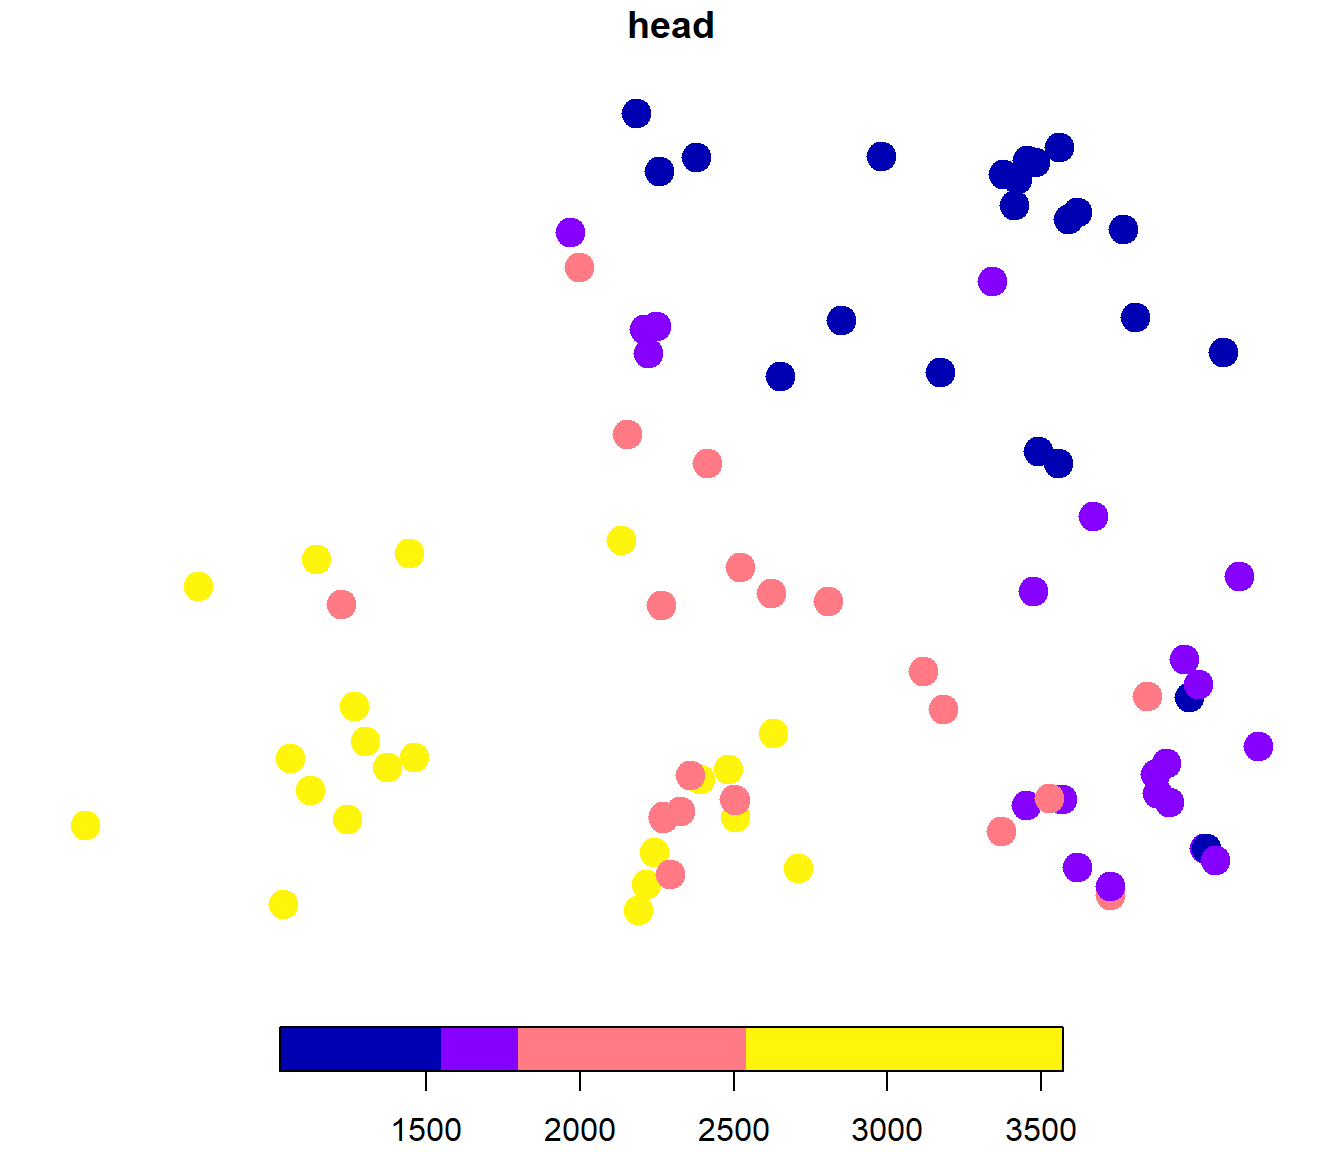
\includegraphics[width=0.7\linewidth]{03-modelado_files/figure-latex/unnamed-chunk-9-1} \end{center}

En el caso de la anisotropía zonal se suele considerar una combinación de un semivariograma isotrópico más otros ``zonales'' que depende solamente de la distancia en ciertas direcciones (o componentes del vector de salto).
Por ejemplo, en el caso bidimensional, si \(\phi\) es la dirección de mayor varianza se suele considerar una combinación de la forma:
\[\gamma(\mathbf{h})=\gamma_1 (\left\| \mathbf{h}\right\|)+\gamma_2(h_{\phi }),\]
siendo \(\gamma_1 (\cdot)\) y \(\gamma_2 (\cdot)\) semivariogramas isotrópicos, y \(h_{\phi } =\cos (\phi)h_1 +\sin(\phi)h_2\) el salto en la dirección \(\phi\), para \(\mathbf{h}=(h_1 ,h_2)\in \mathbb{R} ^{2}\).
Es importante destacar que este tipo de anisotropías pueden causar la aparición de problemas al realizar predicción espacial (ver p.e. Myers y Journel, 1990; y Rouhani y Myers, 1990), como por ejemplo dar lugar a sistemas kriging no válidos con ciertas configuraciones de los datos.
Hay que tener un especial cuidado cuando el covariograma es expresado como suma de covariogramas unidimensionales, en cuyo caso el resultado puede ser únicamente condicionalmente semidefinido positivo sobre un dominio multidimensional.

Este tipo de modelos son casos particulares del modelo lineal de regionalización descrito en la siguiente sección.

Una variante de la anisotropía zonal es el caso de covariogramas separables (también denominados factorizables) en componentes del vector de salto.
Por ejemplo, un covariograma completamente separable en \(\mathbb{R}^2\) es de la forma \(C(h_1, h_2)= C_1(h_1)C_2(h_2)\), siendo \(C_1(\cdot)\) y \(C_2(\cdot)\) covariogramas en \(\mathbb{R}^{1}\).
En este caso se puede pensar que el proceso espacial se obtiene como producto de procesos unidimensionales independientes definidos sobre cada uno de los ejes de coordenadas.
Este tipo de modelos se utilizan habitualmente en geoestadística espacio-temporal (aunque no permiten modelar interacciones).

\hypertarget{vario-lin-reg}{%
\subsection{El modelo lineal de regionalización}\label{vario-lin-reg}}

En \texttt{gstat} se pueden definir modelos de este tipo empleando el parámetro \texttt{add.to} de la función \texttt{vgm()}.

\begin{Shaded}
\begin{Highlighting}[]
\NormalTok{v2 }\OtherTok{\textless{}{-}} \FunctionTok{vgm}\NormalTok{(}\AttributeTok{psill =} \DecValTok{1}\NormalTok{, }\AttributeTok{model =} \StringTok{"Gau"}\NormalTok{, }\AttributeTok{range =} \FloatTok{0.5}\NormalTok{)}
\NormalTok{v12 }\OtherTok{\textless{}{-}} \FunctionTok{vgm}\NormalTok{(}\AttributeTok{psill =} \DecValTok{1}\NormalTok{, }\AttributeTok{model =} \StringTok{"Gau"}\NormalTok{, }\AttributeTok{range =} \FloatTok{0.5}\NormalTok{, }\AttributeTok{add.to =}\NormalTok{ v1)}
\NormalTok{v12}
\end{Highlighting}
\end{Shaded}

\begin{verbatim}
##   model psill range
## 1   Nug     0   0.0
## 2   Exp     1   0.5
## 3   Gau     1   0.5
\end{verbatim}

\begin{Shaded}
\begin{Highlighting}[]
\FunctionTok{plot}\NormalTok{(}\FunctionTok{variogramLine}\NormalTok{(v12, }\AttributeTok{maxdist =} \DecValTok{3}\NormalTok{), }\AttributeTok{type =} \StringTok{"l"}\NormalTok{, }\AttributeTok{ylim =} \FunctionTok{c}\NormalTok{(}\DecValTok{0}\NormalTok{, }\FloatTok{2.25}\NormalTok{))}
\FunctionTok{lines}\NormalTok{(}\FunctionTok{variogramLine}\NormalTok{(v1, }\AttributeTok{maxdist =} \DecValTok{3}\NormalTok{), }\AttributeTok{col =} \StringTok{"red"}\NormalTok{, }\AttributeTok{lty =} \DecValTok{2}\NormalTok{)}
\FunctionTok{lines}\NormalTok{(}\FunctionTok{variogramLine}\NormalTok{(v2, }\AttributeTok{maxdist =} \DecValTok{3}\NormalTok{), }\AttributeTok{col =} \StringTok{"blue"}\NormalTok{, }\AttributeTok{lty =} \DecValTok{3}\NormalTok{)}
\FunctionTok{legend}\NormalTok{(}\StringTok{"bottomright"}\NormalTok{, }\FunctionTok{c}\NormalTok{(}\StringTok{"Exponencial"}\NormalTok{, }\StringTok{"Gaussiano"}\NormalTok{, }\StringTok{"Anidado"}\NormalTok{), }\AttributeTok{lty =} \FunctionTok{c}\NormalTok{(}\DecValTok{2}\NormalTok{, }\DecValTok{3}\NormalTok{, }\DecValTok{1}\NormalTok{), }
       \AttributeTok{col =} \FunctionTok{c}\NormalTok{(}\StringTok{"red"}\NormalTok{, }\StringTok{"blue"}\NormalTok{, }\StringTok{"black"}\NormalTok{), }\AttributeTok{cex =} \FloatTok{0.75}\NormalTok{)}
\end{Highlighting}
\end{Shaded}

\begin{center}\includegraphics[width=0.7\linewidth]{03-modelado_files/figure-latex/unnamed-chunk-10-1} \end{center}

\hypertarget{ajuste-variog}{%
\section{Ajuste de un modelo válido}\label{ajuste-variog}}

\hypertarget{ls-fit}{%
\subsection{Estimación por mínimos cuadrados}\label{ls-fit}}

\hypertarget{ml-fit}{%
\subsection{Estimación por máxima verosimilitud}\label{ml-fit}}

\hypertarget{comentarios-sobre-los-distintos-muxe9todos}{%
\subsection{Comentarios sobre los distintos métodos}\label{comentarios-sobre-los-distintos-muxe9todos}}

\hypertarget{modelado-conjunto-de-la-tendencia-y-del-variograma}{%
\section{Modelado conjunto de la tendencia y del variograma}\label{modelado-conjunto-de-la-tendencia-y-del-variograma}}

Si no se puede asumir que la tendencia es constante, para poder estimarla de forma eficiente sería necesario conocer la dependencia (i.e.~conocer \(\gamma(\cdot)\)).
Este problema circular se suele resolver en la práctica realizando el paso 2 de forma iterativa, como se describe en la Sección 3.4.
Otra alternativa sería asumir normalidad y estimar ambos componentes de forma conjunta empleando alguno de los métodos basados en máxima verosimilitud descritos en la Sección \ref{ml-fit}.

\hypertarget{kriging}{%
\chapter{Predicción Kriging}\label{kriging}}

\textbf{\emph{En preparación\ldots{}}}

En este capítulo se comentan brevemente los métodos más conocidos de predicción espacial denominados métodos kriging\footnote{Podríamos definir los métodos kriging como algoritmos de predicción de mínimo error en media cuadrática que tienen en cuenta la estructura de segundo orden del proceso.} (ver Sección 1.2.1 para un resumen del origen de esta terminología), centrándonos únicamente en el caso de predicción lineal puntual univariante (el caso multivariante se trata en el Capítulo 5).
Una revisión más completa de estos métodos se tiene por ejemplo en Cressie (1993, Capítulo 3 y secciones 5.1, 5.4 y 5.9.1) o Chilès y Delfiner (1999, capítulos 3, 4 y 6).

\hypertarget{introducciuxf3n}{%
\section{Introducción}\label{introducciuxf3n}}

Si denotamos por \(\mathbf{Z}=\left( Z(\mathbf{s}_{1} ), \ldots, z(\mathbf{s}_{n} )\right)^\top\) valores observados del proceso, los distintos métodos kriging proporcionan un predictor \(p(\mathbf{Z},\mathbf{s}_{0} )\) de \(Z(\mathbf{s}_{0} )\) verificando que:

\begin{itemize}
\item
  es lineal:
  \[p(\mathbf{Z},\mathbf{s}_{0} )=\sum\limits_{i=1}^{n}\lambda_{i} Z(\mathbf{s}_{i} ) +\lambda_{0},\]
\item
  es uniformemente insesgado, para cualquier \(\mu(\cdot)\):
  \[E(p(\mathbf{Z},\mathbf{s}_{0} ))=\mu(\mathbf{s}_{0} ),\]
\item
  y minimiza el error en media cuadrática (e.m.c.) de predicción\footnote{Como es bien sabido, en el caso de normalidad el predictor óptimo (tomando como función de pérdidas el error cuadrático) es lineal y va a coincidir con los predictores kriging. Pero si el proceso no es normal no tiene porque serlo, lo que ha motivado el desarrollo de métodos kriging no lineales (ver p.e. Rivoirard, 1994) y del kriging trans-normal (ver sección 4.X).}:
  \[E\left( \left( p(\mathbf{Z},\mathbf{s}_{0} )-Z(\mathbf{s}_{0} )\right)^{\text{2} } \right),\]
\end{itemize}

(al hablar de predicción óptima nos referiremos a que se verifican estas dos últimas condiciones).

Dependiendo de las suposiciones acerca de la función de tendencia \(\mu(\cdot)\), se distingue principalmente entre tres métodos kriging:

\begin{enumerate}
\def\labelenumi{\arabic{enumi}.}
\item
  \emph{Kriging simple} (KS): se supone que la media es conocida (algunos autores suponen también que es constante o incluso cero).
  Además se asume que el covariograma existe y es conocido.
\item
  \emph{Kriging ordinario} (KO): se supone que la media es constante (i.e.~\(E(Z(\mathbf{s}))=\mu ,\forall \mathbf{s}\in D\)) y desconocida.
  Además se asume que por lo menos existe el variograma y es conocido.
\item
  \emph{Kriging universal} (KU; también denominado kriging con modelo de tendencia): se supone que la media es desconocida y no constante, pero
  que es una combinación lineal (desconocida) de \(p+1\) funciones (o variables explicativas) conocidas \(\left\{ x_{j} (\cdot):j=0, \ldots,p\right\}\):
  \[\mu(\mathbf{s})=\sum\limits_{j=0}^{p}x_{j} (\mathbf{s})\beta_{j}\]
  donde \(?=(\beta_{0} , \ldots,\beta_{p} )^\top \in \mathbb{R}^{p+1}\) es un vector desconocido.
  Se asume también que por lo menos existe el variograma y es conocido\footnote{Siempre que una de las funciones explicativas sea idénticamente 1, p.e. \(x_{0} (\cdot)\equiv 1\), en caso contrario las ecuaciones kriging sólo pueden expresarse en función del covariograma.}.
\end{enumerate}

Por simplicidad el kriging ordinario se tratará en este capítulo como un caso particular del kriging universal (aunque en la práctica se suele
pensar en el KO como un método distinto al KU, principalmente por ciertos inconvenientes que presenta este último; ver Sección 4.X.X).

\hypertarget{ksimple}{%
\section{Kriging con media conocida: kriging simple}\label{ksimple}}

\hypertarget{kuniversal}{%
\section{Kriging con media desconocida: kriging universal}\label{kuniversal}}

\hypertarget{consideraciones-kriging}{%
\section{Consideraciones acerca de los métodos kriging}\label{consideraciones-kriging}}

\hypertarget{multivar}{%
\chapter{Procesos espaciales multivariantes}\label{multivar}}

\textbf{\emph{En preparación\ldots{}}}

Si \(\left\{ Z_{j}(\mathbf{s}):j=1, \ldots, k;\mathbf{s}\in D\right\}\)
son \(k\) procesos espaciales univariantes (y que se suponen en principio interdependientes), el vector
\[\mathbf{Z}(\mathbf{s})=(Z_{1}(\mathbf{s}), \ldots, Z_{k}(\mathbf{s}))^\top\]
lo denominaremos proceso espacial multivariante (también se denomina proceso espacial vectorial, campo vectorial espacial o vector regionalizado).

\hypertarget{esp-temp}{%
\chapter{Procesos espaciales espacio-temporales}\label{esp-temp}}

\textbf{\emph{En preparación\ldots{}}}

Como ya se comentó en el Capítulo 1 se puede pensar en un procesos espacio-temporal como un caso particular de un proceso espacial en el que una de las componentes es el tiempo.
Sin embargo, para enfatizar el carácter temporal, se utilizará una notación de la forma:
\[\left\{ Z(\mathbf{s},t):(\mathbf{s},t)\in D\times T\right\}\]
donde \(D\times T\subset \mathbb{R} ^{d} \times \mathbb{R}^{+,0}\), para
referirse a un proceso espacio-temporal.

En algunos casos los procesos espacio-temporales son modelados también
como procesos espaciales multivariantes (e.g.~Egbert y Lettenmaier,
1986; Kyriakidis y Journel, 1999).

Por ejemplo, se puede considerar una representación de la forma:

\[Z(\mathbf{s},t)=\mathbf{Z}(\mathbf{s})=(Z_{1} (\mathbf{s}), \ldots,Z_{k} (
\mathbf{s}))^\top,\]
donde
\[Z_{i} (\mathbf{s})=Z(\mathbf{s},t_{i} ),\  i=1, \ldots,k.\]
O también:
\[Z(\mathbf{s},t) = \mathbf{Z}(t) =  \left(Z_{1}(t), \ldots, Z_{n}(t) \right)^\top,\]
siendo
\[Z_{j} (t)=Z(\mathbf{s}_{j} ,t),\  j=1, \ldots,n.\]
Uno de los principales problemas al utilizar estas aproximaciones es que, utilizando los modelos geoestadísticos tradicionales, no es posible la
predicción en todas las posiciones espacio-temporales sin algún tipo de
modelado adicional. Por ejemplo, utilizando la representación y los métodos geoestadísticos de predicción espacial multivariante, se pueden obtener en principio superficies de predicción solamente en los k instantes temporales \(t_{i} ,\  i=1, \ldots, k\),
y no es posible la interpolación temporal sin modelado adicional (ver Sección 5.3.5).

\hypertarget{appendix-apendices}{%
\appendix}


\hypertarget{intro-sp}{%
\chapter{\texorpdfstring{Introducción al paquete \textbf{sp}}{Introducción al paquete sp}}\label{intro-sp}}

El paquete \href{https://CRAN.R-project.org/package=sp}{\texttt{sp}} {[}Classes and methods for spatial data; \protect\hyperlink{ref-Pebesma2005}{E. J. Pebesma y Bivand} (\protect\hyperlink{ref-Pebesma2005}{2005}){]} implementa objetos y métodos para datos espaciales\ldots{}

Introducción, para más detalles ver \protect\hyperlink{ref-Bivand2013}{Bivand et~al.} (\protect\hyperlink{ref-Bivand2013}{2013})\ldots{}
\url{https://www.maths.lancs.ac.uk/~rowlings/Teaching/UseR2012/cheatsheet.html}

\hypertarget{tipos-de-objetos}{%
\section{Tipos de objetos}\label{tipos-de-objetos}}

\begin{Shaded}
\begin{Highlighting}[]
\CommentTok{\# Librería sp:classes and methods for spatial data}
\FunctionTok{library}\NormalTok{(sp) }\CommentTok{\# install.packages(\textquotesingle{}sp\textquotesingle{})}

\CommentTok{\# Tipos de objetos}
\FunctionTok{getClass}\NormalTok{(}\StringTok{"Spatial"}\NormalTok{)}
\end{Highlighting}
\end{Shaded}

\begin{verbatim}
## Class "Spatial" [package "sp"]
## 
## Slots:
##                               
## Name:         bbox proj4string
## Class:      matrix         CRS
## 
## Known Subclasses: 
## Class "SpatialPoints", directly
## Class "SpatialMultiPoints", directly
## Class "SpatialGrid", directly
## Class "SpatialLines", directly
## Class "SpatialPolygons", directly
## Class "SpatialPointsDataFrame", by class "SpatialPoints", distance 2
## Class "SpatialPixels", by class "SpatialPoints", distance 2
## Class "SpatialMultiPointsDataFrame", by class "SpatialMultiPoints", distance 2
## Class "SpatialGridDataFrame", by class "SpatialGrid", distance 2
## Class "SpatialLinesDataFrame", by class "SpatialLines", distance 2
## Class "SpatialPixelsDataFrame", by class "SpatialPoints", distance 3
## Class "SpatialPolygonsDataFrame", by class "SpatialPolygons", distance 2
\end{verbatim}

\begin{itemize}
\item
  Clases del tipo S4 (definicion formal con componentes
  denominadas slots)
\item
  Tipo base: \texttt{Spatial}

  \begin{itemize}
  \item
    \texttt{bbox} (bounding box): matriz con los límites mínimo y máximo de
    las coordenadas (principalmente para representación gráfica;
    normalmente se genera automáticamente).
  \item
    \texttt{proj4string}: cadena de texto que define el sistema de
    coordenadas de referencia (realmente objeto tipo \emph{CRS,}
    coordinate reference system) en formato
    \href{http://trac.osgeo.org/proj}{PROJ.4}.

    \begin{itemize}
    \item
      \texttt{CRS(as.character(NA))} para indicar no disponible/faltante
    \item
      \texttt{CRS(+proj=longlat)} para coordenadas geográficas
    \item
      \texttt{CRS(+proj=longlat\ +ellps=WGS84)} estándar GPS (World
      Geodetic System of 1984)
    \end{itemize}
  \end{itemize}
\end{itemize}

\begin{Shaded}
\begin{Highlighting}[]
\NormalTok{xbbox }\OtherTok{\textless{}{-}} \FunctionTok{matrix}\NormalTok{( }\FunctionTok{c}\NormalTok{(}\DecValTok{0}\NormalTok{,}\DecValTok{0}\NormalTok{,}\DecValTok{1}\NormalTok{,}\DecValTok{1}\NormalTok{), }\AttributeTok{ncol=}\DecValTok{2}\NormalTok{)}
\FunctionTok{colnames}\NormalTok{(xbbox) }\OtherTok{\textless{}{-}} \FunctionTok{c}\NormalTok{(}\StringTok{"min"}\NormalTok{, }\StringTok{"max"}\NormalTok{) }\CommentTok{\# Normalmente la bbox se genera automáticamente al crear el objeto}
\NormalTok{x }\OtherTok{\textless{}{-}} \FunctionTok{Spatial}\NormalTok{(xbbox, }\AttributeTok{proj4string =} \FunctionTok{CRS}\NormalTok{(}\FunctionTok{as.character}\NormalTok{(}\ConstantTok{NA}\NormalTok{)))}
\NormalTok{x}
\end{Highlighting}
\end{Shaded}

\begin{verbatim}
## An object of class "Spatial"
## Slot "bbox":
##      min max
## [1,]   0   1
## [2,]   0   1
## 
## Slot "proj4string":
## Coordinate Reference System:
## Deprecated Proj.4 representation: NA
\end{verbatim}

Los objetos son del tipo S4.
Los componentes se denominan slots.
Se acceden con la función \texttt{slot()} o el operador \texttt{@}.

\begin{Shaded}
\begin{Highlighting}[]
\FunctionTok{slot}\NormalTok{(x,}\StringTok{\textquotesingle{}bbox\textquotesingle{}}\NormalTok{)}
\end{Highlighting}
\end{Shaded}

\begin{verbatim}
##      min max
## [1,]   0   1
## [2,]   0   1
\end{verbatim}

\begin{Shaded}
\begin{Highlighting}[]
\NormalTok{x}\SpecialCharTok{@}\NormalTok{bbox }\DocumentationTok{\#\#\# en s4 se pone @ en vez de $.}
\end{Highlighting}
\end{Shaded}

\begin{verbatim}
##      min max
## [1,]   0   1
## [2,]   0   1
\end{verbatim}

El paquete sp dispone también de funciones para acceder/establecer
los componentes:

\begin{Shaded}
\begin{Highlighting}[]
\FunctionTok{bbox}\NormalTok{(x)}
\end{Highlighting}
\end{Shaded}

\begin{verbatim}
##      min max
## [1,]   0   1
## [2,]   0   1
\end{verbatim}

\begin{Shaded}
\begin{Highlighting}[]
\FunctionTok{proj4string}\NormalTok{(x) }\OtherTok{\textless{}{-}} \FunctionTok{CRS}\NormalTok{(}\StringTok{"+proj=longlat +ellps=WGS84"}\NormalTok{) }\CommentTok{\# Importante}
\end{Highlighting}
\end{Shaded}

\hypertarget{spatialpoints-y-spatialpointsdataframe}{%
\subsection{SpatialPoints y SpatialPointsDataFrame}\label{spatialpoints-y-spatialpointsdataframe}}

\begin{itemize}
\item
  Tipo \texttt{SpatialPoints}

  \begin{itemize}
  \item
    Slots: \texttt{coords,\ bbox,\ proj4string}
  \item
    Objeto de datos básico para procesos puntuales.
  \end{itemize}
\item
  Tipo \texttt{SpatialPointsDataFrame}

  \begin{itemize}
  \item
    Slots: \texttt{data,\ coords.nrs,\ coords,\ bbox,\ proj4string}
  \item
    Objeto de datos básico para procesos geoestadísticos (y procesos
    puntuales marcados).
  \end{itemize}
\end{itemize}

\hypertarget{ejemplo-spatialpoints}{%
\subsubsection{Ejemplo SpatialPoints}\label{ejemplo-spatialpoints}}

\begin{Shaded}
\begin{Highlighting}[]
\FunctionTok{load}\NormalTok{(}\StringTok{"datos/caballa.galicia.RData"}\NormalTok{)}
\FunctionTok{str}\NormalTok{(caballa.galicia)  }\CommentTok{\# data.frame(attr(caballa.galicia, "variable.labels"))}
\end{Highlighting}
\end{Shaded}

\begin{verbatim}
## 'data.frame':    676 obs. of  12 variables:
##  $ id       : Factor w/ 31 levels "A1","A2","B1",..: 17 17 19 19 19 21 21 23 23 23 ...
##  $ x        : num  -9.4 -9.44 -9.44 -9.4 -9.47 ...
##  $ y        : num  43 43 43 43 42.8 ...
##  $ fecha    : num  1.32e+10 1.32e+10 1.32e+10 1.32e+10 1.32e+10 ...
##  $ semana   : num  7 7 7 7 7 7 8 8 8 8 ...
##  $ mes      : num  2 2 2 2 2 2 2 2 2 2 ...
##  $ ano      : num  2001 2001 2001 2001 2001 ...
##  $ cpue     : num  18 240 240 18 118 ...
##  $ chl_a    : num  NA NA 7.08 7.08 7.08 ...
##  $ sust_amar: num  NA NA 0.356 0.356 0.356 ...
##  $ sst      : num  14.2 14.2 16 16 16 16.1 16 15.9 15.9 15.9 ...
##  $ lcpue    : num  2.89 5.48 5.48 2.89 4.77 ...
##  - attr(*, "variable.labels")= Named chr [1:12] "Cuadricula " "" "" "" ...
##   ..- attr(*, "names")= chr [1:12] "id" "x" "y" "fecha" ...
##  - attr(*, "codepage")= int 1252
\end{verbatim}

\begin{Shaded}
\begin{Highlighting}[]
\FunctionTok{plot}\NormalTok{(y}\SpecialCharTok{\textasciitilde{}}\NormalTok{x, }\AttributeTok{data =}\NormalTok{ caballa.galicia)}
\end{Highlighting}
\end{Shaded}

\begin{center}\includegraphics[width=0.7\linewidth]{11-sp_files/figure-latex/unnamed-chunk-6-1} \end{center}

\begin{Shaded}
\begin{Highlighting}[]
\NormalTok{spt }\OtherTok{\textless{}{-}} \FunctionTok{SpatialPoints}\NormalTok{(caballa.galicia[,}\FunctionTok{c}\NormalTok{(}\StringTok{"x"}\NormalTok{,}\StringTok{"y"}\NormalTok{)], }\AttributeTok{proj4string =} \FunctionTok{CRS}\NormalTok{(}\StringTok{"+proj=longlat +ellps=WGS84"}\NormalTok{))}
\FunctionTok{summary}\NormalTok{(spt)}
\end{Highlighting}
\end{Shaded}

\begin{verbatim}
## Object of class SpatialPoints
## Coordinates:
##        min       max
## x -9.56538 -8.030065
## y 41.86240 44.010800
## Is projected: FALSE 
## proj4string : [+proj=longlat +ellps=WGS84 +no_defs]
## Number of points: 676
\end{verbatim}

\begin{Shaded}
\begin{Highlighting}[]
\FunctionTok{str}\NormalTok{(spt)}
\end{Highlighting}
\end{Shaded}

\begin{verbatim}
## Formal class 'SpatialPoints' [package "sp"] with 3 slots
##   ..@ coords     : num [1:676, 1:2] -9.4 -9.44 -9.44 -9.4 -9.47 ...
##   .. ..- attr(*, "dimnames")=List of 2
##   .. .. ..$ : chr [1:676] "1" "2" "3" "4" ...
##   .. .. ..$ : chr [1:2] "x" "y"
##   ..@ bbox       : num [1:2, 1:2] -9.57 41.86 -8.03 44.01
##   .. ..- attr(*, "dimnames")=List of 2
##   .. .. ..$ : chr [1:2] "x" "y"
##   .. .. ..$ : chr [1:2] "min" "max"
##   ..@ proj4string:Formal class 'CRS' [package "sp"] with 1 slot
##   .. .. ..@ projargs: chr "+proj=longlat +ellps=WGS84 +no_defs"
##   .. .. ..$ comment: chr "GEOGCRS[\"unknown\",\n    DATUM[\"Unknown based on WGS84 ellipsoid\",\n        ELLIPSOID[\"WGS 84\",6378137,298"| __truncated__
\end{verbatim}

Hay muchos métodos (funciones genéricas) implementados para objetos \texttt{sp}:

\begin{Shaded}
\begin{Highlighting}[]
\CommentTok{\# plot(spt)}
\FunctionTok{plot}\NormalTok{(spt, }\AttributeTok{axes=}\ConstantTok{TRUE}\NormalTok{)}
\end{Highlighting}
\end{Shaded}

\begin{center}\includegraphics[width=0.7\linewidth]{11-sp_files/figure-latex/unnamed-chunk-7-1} \end{center}

\hypertarget{ejemplo-spatialpointsdataframe}{%
\subsubsection{Ejemplo SpatialPointsDataFrame}\label{ejemplo-spatialpointsdataframe}}

Importante (para preparar datos):

\begin{Shaded}
\begin{Highlighting}[]
\NormalTok{sdf1 }\OtherTok{\textless{}{-}} \FunctionTok{SpatialPointsDataFrame}\NormalTok{(caballa.galicia[,}\FunctionTok{c}\NormalTok{(}\DecValTok{2}\NormalTok{,}\DecValTok{3}\NormalTok{)], caballa.galicia[,}\SpecialCharTok{{-}}\FunctionTok{c}\NormalTok{(}\DecValTok{2}\NormalTok{,}\DecValTok{3}\NormalTok{)], }\AttributeTok{proj4string =} \FunctionTok{CRS}\NormalTok{(}\StringTok{"+proj=longlat +ellps=WGS84"}\NormalTok{))}
\FunctionTok{str}\NormalTok{(sdf1)}
\end{Highlighting}
\end{Shaded}

\begin{verbatim}
## Formal class 'SpatialPointsDataFrame' [package "sp"] with 5 slots
##   ..@ data       :'data.frame':  676 obs. of  10 variables:
##   .. ..$ id       : Factor w/ 31 levels "A1","A2","B1",..: 17 17 19 19 19 21 21 23 23 23 ...
##   .. ..$ fecha    : num [1:676] 1.32e+10 1.32e+10 1.32e+10 1.32e+10 1.32e+10 ...
##   .. ..$ semana   : num [1:676] 7 7 7 7 7 7 8 8 8 8 ...
##   .. ..$ mes      : num [1:676] 2 2 2 2 2 2 2 2 2 2 ...
##   .. ..$ ano      : num [1:676] 2001 2001 2001 2001 2001 ...
##   .. ..$ cpue     : num [1:676] 18 240 240 18 118 ...
##   .. ..$ chl_a    : num [1:676] NA NA 7.08 7.08 7.08 ...
##   .. ..$ sust_amar: num [1:676] NA NA 0.356 0.356 0.356 ...
##   .. ..$ sst      : num [1:676] 14.2 14.2 16 16 16 16.1 16 15.9 15.9 15.9 ...
##   .. ..$ lcpue    : num [1:676] 2.89 5.48 5.48 2.89 4.77 ...
##   ..@ coords.nrs : num(0) 
##   ..@ coords     : num [1:676, 1:2] -9.4 -9.44 -9.44 -9.4 -9.47 ...
##   .. ..- attr(*, "dimnames")=List of 2
##   .. .. ..$ : chr [1:676] "1" "2" "3" "4" ...
##   .. .. ..$ : chr [1:2] "x" "y"
##   ..@ bbox       : num [1:2, 1:2] -9.57 41.86 -8.03 44.01
##   .. ..- attr(*, "dimnames")=List of 2
##   .. .. ..$ : chr [1:2] "x" "y"
##   .. .. ..$ : chr [1:2] "min" "max"
##   ..@ proj4string:Formal class 'CRS' [package "sp"] with 1 slot
##   .. .. ..@ projargs: chr "+proj=longlat +ellps=WGS84 +no_defs"
##   .. .. ..$ comment: chr "GEOGCRS[\"unknown\",\n    DATUM[\"Unknown based on WGS84 ellipsoid\",\n        ELLIPSOID[\"WGS 84\",6378137,298"| __truncated__
\end{verbatim}

Una alernativa normalmente preferible es modificar directamente
el \texttt{data.frame}:

\begin{Shaded}
\begin{Highlighting}[]
\NormalTok{sdf }\OtherTok{\textless{}{-}}\NormalTok{ caballa.galicia}
\FunctionTok{coordinates}\NormalTok{(sdf) }\OtherTok{\textless{}{-}} \FunctionTok{c}\NormalTok{(}\StringTok{"x"}\NormalTok{, }\StringTok{"y"}\NormalTok{) }\CommentTok{\# Recomendación}
\FunctionTok{proj4string}\NormalTok{(sdf) }\OtherTok{\textless{}{-}} \FunctionTok{CRS}\NormalTok{(}\StringTok{"+proj=longlat +ellps=WGS84"}\NormalTok{)  }\CommentTok{\# También sdf@proj4string \textless{}{-} CRS("+proj=longlat +ellps=WGS84")}
\FunctionTok{str}\NormalTok{(sdf)}
\end{Highlighting}
\end{Shaded}

\begin{verbatim}
## Formal class 'SpatialPointsDataFrame' [package "sp"] with 5 slots
##   ..@ data       :'data.frame':  676 obs. of  10 variables:
##   .. ..$ id       : Factor w/ 31 levels "A1","A2","B1",..: 17 17 19 19 19 21 21 23 23 23 ...
##   .. ..$ fecha    : num [1:676] 1.32e+10 1.32e+10 1.32e+10 1.32e+10 1.32e+10 ...
##   .. ..$ semana   : num [1:676] 7 7 7 7 7 7 8 8 8 8 ...
##   .. ..$ mes      : num [1:676] 2 2 2 2 2 2 2 2 2 2 ...
##   .. ..$ ano      : num [1:676] 2001 2001 2001 2001 2001 ...
##   .. ..$ cpue     : num [1:676] 18 240 240 18 118 ...
##   .. ..$ chl_a    : num [1:676] NA NA 7.08 7.08 7.08 ...
##   .. ..$ sust_amar: num [1:676] NA NA 0.356 0.356 0.356 ...
##   .. ..$ sst      : num [1:676] 14.2 14.2 16 16 16 16.1 16 15.9 15.9 15.9 ...
##   .. ..$ lcpue    : num [1:676] 2.89 5.48 5.48 2.89 4.77 ...
##   ..@ coords.nrs : int [1:2] 2 3
##   ..@ coords     : num [1:676, 1:2] -9.4 -9.44 -9.44 -9.4 -9.47 ...
##   .. ..- attr(*, "dimnames")=List of 2
##   .. .. ..$ : chr [1:676] "1" "2" "3" "4" ...
##   .. .. ..$ : chr [1:2] "x" "y"
##   ..@ bbox       : num [1:2, 1:2] -9.57 41.86 -8.03 44.01
##   .. ..- attr(*, "dimnames")=List of 2
##   .. .. ..$ : chr [1:2] "x" "y"
##   .. .. ..$ : chr [1:2] "min" "max"
##   ..@ proj4string:Formal class 'CRS' [package "sp"] with 1 slot
##   .. .. ..@ projargs: chr "+proj=longlat +ellps=WGS84 +no_defs"
##   .. .. ..$ comment: chr "GEOGCRS[\"unknown\",\n    DATUM[\"Unknown based on WGS84 ellipsoid\",\n        ELLIPSOID[\"WGS 84\",6378137,298"| __truncated__
\end{verbatim}

Operaciones como en un \texttt{data.frame}.

\begin{Shaded}
\begin{Highlighting}[]
\FunctionTok{names}\NormalTok{(sdf)}
\end{Highlighting}
\end{Shaded}

\begin{verbatim}
##  [1] "id"        "fecha"     "semana"    "mes"       "ano"       "cpue"     
##  [7] "chl_a"     "sust_amar" "sst"       "lcpue"
\end{verbatim}

\begin{Shaded}
\begin{Highlighting}[]
\NormalTok{sdf}\SpecialCharTok{$}\NormalTok{id  }\CommentTok{\# Equivalente a sdf@data$id }
\end{Highlighting}
\end{Shaded}

\begin{verbatim}
##   [1] E2 E2 F2 F2 F2 G2 G2 H1 H1 H1 I1 I1 I2 I2 J1 J1 J1 J1 J2 J2 J2 D1 E1 F1 F1
##  [26] G1 G2 H2 I2 I2 J1 J2 D1 E2 E2 F2 F1 F1 F1 F2 G1 G1 G2 G2 H2 I1 I1 I2 I2 I2
##  [51] J1 J1 J2 E2 F1 F1 G1 G2 H1 H2 H2 I1 I1 I1 I1 I2 I2 I2 F1 F2 F2 G2 I1 I1 I1
##  [76] I1 I2 I2 I2 I2 J1 J1 E2 F2 F2 F2 F2 G2 G2 H3 I3 I3 I3 J3 J3 J3 F2 G2 H2 F2
## [101] G2 G2 H2 I1 I1 I2 I2 J2 B2 B3 C2 C3 C3 E2 F2 F2 G2 H3 I3 B3 B3 C3 C3 C3 C4
## [126] C4 C4 I2 I2 I3 J2 J2 H2 H2 H2 I2 I2 I2 E2 F2 F2 G2 B2 B3 B3 C3 C3 C3 C4 C4
## [151] E1 F1 F1 F1 F2 G1 G1 G2 E1 F1 F2 G2 G2 H2 I2 I2 I2 J2 J2 A1 B2 B3 B3 B3 B4
## [176] B4 C3 I2 I2 J2 J2 I2 J2 I2 J2 I3 J2 J3 A1 A2 A2 B3 B4 B4 B5 C2 C3 C3 C4 D2
## [201] D3 F1 F2 C2 C2 C3 C3 C3 C4 C4 D4 H2 H2 H3 I3 B2 B3 C2 C2 C3 C3 C3 C3 C4 B2
## [226] B3 C2 C3 C3 C3 C3 C4 C4 C4 B2 C2 C2 C3 C3 C3 C3 C4 C4 C4 H2 H2 I1 I2 I2 I1
## [251] I2 I2 I2 I2 I3 J1 J2 J2 J2 J3 B2 B3 B3 B3 B3 C3 C3 C3 C3 C4 C4 C4 I2 I2 I3
## [276] I3 J2 J2 J3 J3 B2 C3 C3 C4 C4 B2 B2 B3 B3 B3 C3 C3 C3 C4 C4 B2 B2 B3 C3 C3
## [301] C3 C3 C4 D4 B2 B2 B3 C2 C2 C3 C3 C3 C3 C4 I2 J2 J2 J2 B2 B3 C2 C2 C3 C3 C4
## [326] I3 J2 J2 J3 B3 B3 B3 B4 B4 C3 C4 C4 B2 B3 C3 C3 C3 C4 C4 B3 C3 C3 C4 C4 C4
## [351] B3 B3 B3 B4 B4 C4 G2 H1 H2 H2 B3 B3 B4 C4 C4 H2 H2 I2 I2 H2 I2 J2 B3 B3 B4
## [376] C3 C4 C4 D4 B3 C3 C3 C4 C4 C4 D4 D4 H2 I2 I2 J1 J2 D1 D2 D2 D2 D2 H2 I2 E2
## [401] F2 F2 F2 E2 E2 F2 F2 E2 F2 F2 F2 G2 B2 B2 B3 B3 B3 C3 C3 C3 C4 C1 C2 C3 C3
## [426] C4 D1 D2 D4 C1 C2 C2 C3 C3 C4 I2 I2 J1 J1 J2 J2 I3 H2 H3 I2 I2 I2 I2 I2 I3
## [451] J1 J1 J1 J2 J2 J2 J2 H3 H3 I2 I3 I3 I3 I3 I3 J2 J2 J3 H3 H3 H3 I2 I2 I2 I3
## [476] I3 I3 J2 J2 G3 G3 H2 H2 H2 H2 H2 H3 G3 H2 H2 H2 E1 F1 E1 F1 E1 F1 G2 H1 H2
## [501] H2 H3 I3 C2 D1 D1 D1 D2 D2 D2 E2 E2 E2 F2 B1 B2 C2 C2 C3 D1 D1 D1 D2 E2 E2
## [526] H2 I2 I2 I2 J1 J1 J1 J2 J2 H3 H3 I3 I3 I3 I3 J3 J3 H1 I1 H3 H3 I2 I2 I3 I3
## [551] I3 I3 J2 J2 I2 I3 J2 H3 H3 I3 I3 I3 I3 J3 J3 H3 I3 I3 I3 J3 J3 H3 H3 I2 I3
## [576] I3 I3 I3 J3 J3 H3 H3 I2 I3 I3 I3 J2 J2 J3 F1 F2 G2 G2 H1 H2 H2 F1 G1 G2 I1
## [601] I2 I2 I2 J1 J1 J2 J2 J2 I2 I2 I2 I2 J2 J2 J2 J2 D1 D2 E2 E2 E2 F2 F2 G2 D1
## [626] D1 D1 D1 D2 D2 E1 E2 E2 F1 G1 G2 G2 F1 G1 G1 G1 G2 G2 G1 G2 H3 I2 I3 I3 J2
## [651] J2 J3 J3 H3 I3 I3 I3 I3 I3 J2 J3 J3 J3 J3 H3 I2 I3 I3 I3 I3 I3 I3 J3 J3 J3
## [676] J3
## 31 Levels: A1 A2 B1 B2 B3 B4 B5 C1 C2 C3 C4 D1 D2 D3 D4 E1 E2 F1 F2 G1 ... J3
\end{verbatim}

\begin{Shaded}
\begin{Highlighting}[]
\FunctionTok{plot}\NormalTok{(sdf, }\AttributeTok{axes =} \ConstantTok{TRUE}\NormalTok{)}
\FunctionTok{plot}\NormalTok{(sdf[sdf}\SpecialCharTok{$}\NormalTok{id }\SpecialCharTok{==} \StringTok{"J3"}\NormalTok{, ], }\AttributeTok{col =} \StringTok{"red"}\NormalTok{, }\AttributeTok{add =} \ConstantTok{TRUE}\NormalTok{)}
\end{Highlighting}
\end{Shaded}

\begin{center}\includegraphics[width=0.7\linewidth]{11-sp_files/figure-latex/unnamed-chunk-10-1} \end{center}

Importante (para análisis descriptivo):

\begin{Shaded}
\begin{Highlighting}[]
\FunctionTok{summary}\NormalTok{(sdf[,}\FunctionTok{c}\NormalTok{(}\StringTok{"cpue"}\NormalTok{,}\StringTok{"lcpue"}\NormalTok{)])}
\end{Highlighting}
\end{Shaded}

\begin{verbatim}
## Object of class SpatialPointsDataFrame
## Coordinates:
##        min       max
## x -9.56538 -8.030065
## y 41.86240 44.010800
## Is projected: FALSE 
## proj4string : [+proj=longlat +ellps=WGS84 +no_defs]
## Number of points: 676
## Data attributes:
##       cpue              lcpue        
##  Min.   :  0.1435   Min.   :-1.9411  
##  1st Qu.:  1.9559   1st Qu.: 0.6708  
##  Median :  5.8537   Median : 1.7671  
##  Mean   : 30.9208   Mean   : 1.9087  
##  3rd Qu.: 19.5349   3rd Qu.: 2.9722  
##  Max.   :870.0000   Max.   : 6.7685
\end{verbatim}

\begin{Shaded}
\begin{Highlighting}[]
\FunctionTok{hist}\NormalTok{(sdf}\SpecialCharTok{$}\NormalTok{cpue)}
\end{Highlighting}
\end{Shaded}

\begin{center}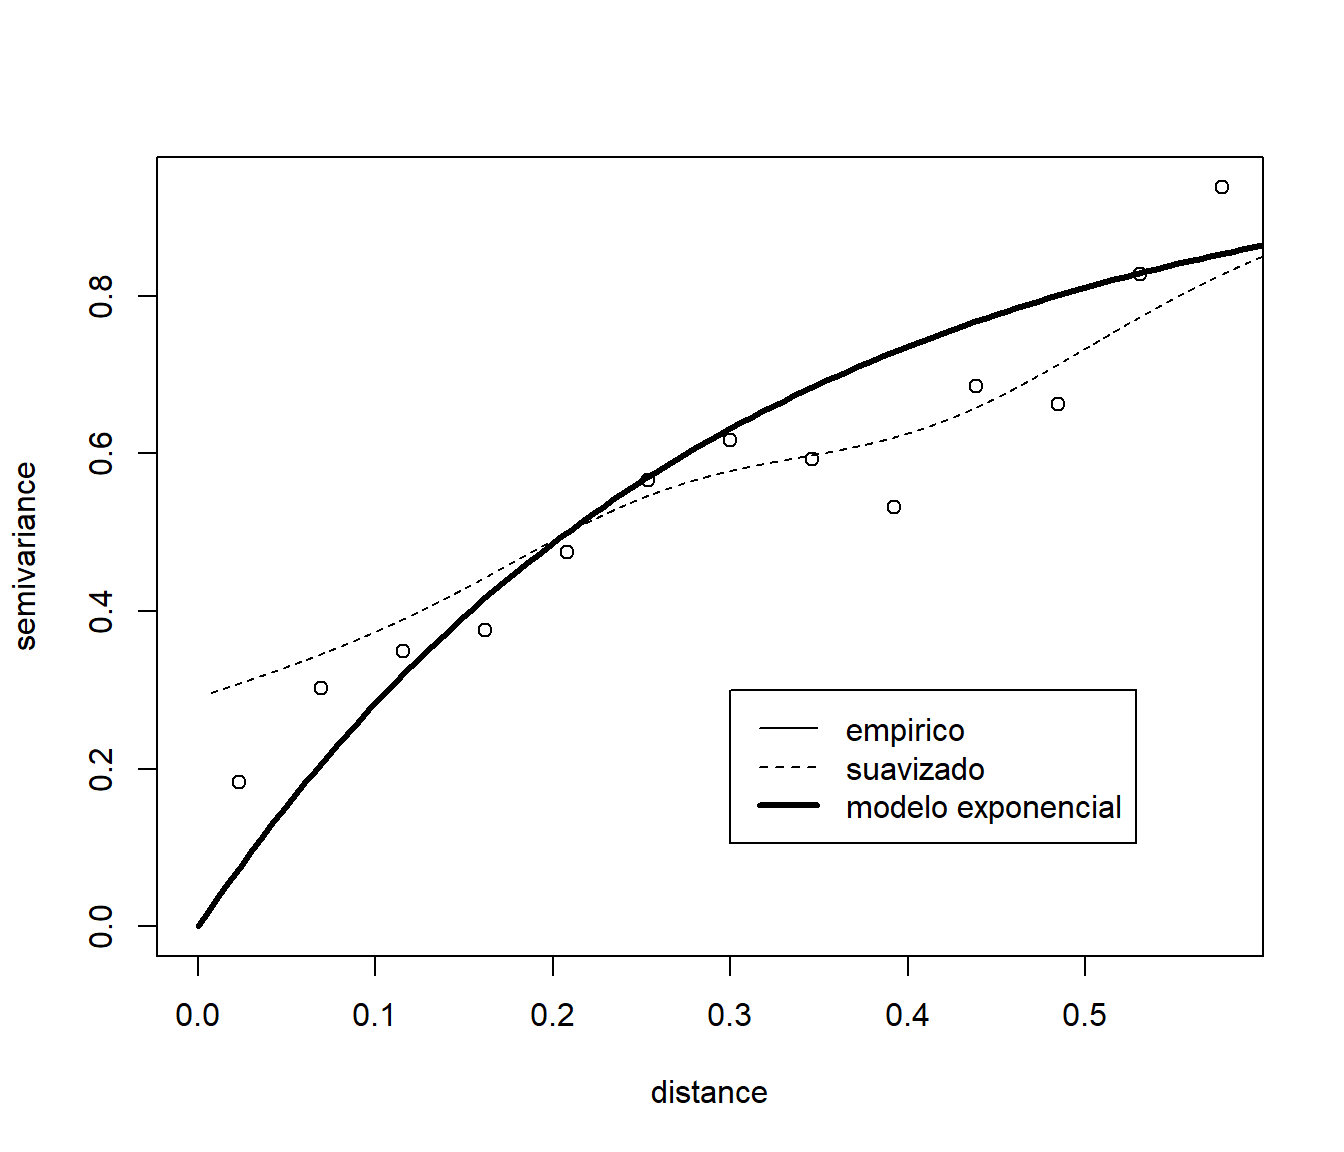
\includegraphics[width=0.7\linewidth]{11-sp_files/figure-latex/unnamed-chunk-11-1} \end{center}

\begin{Shaded}
\begin{Highlighting}[]
\FunctionTok{hist}\NormalTok{(sdf}\SpecialCharTok{$}\NormalTok{lcpue)}
\end{Highlighting}
\end{Shaded}

\begin{center}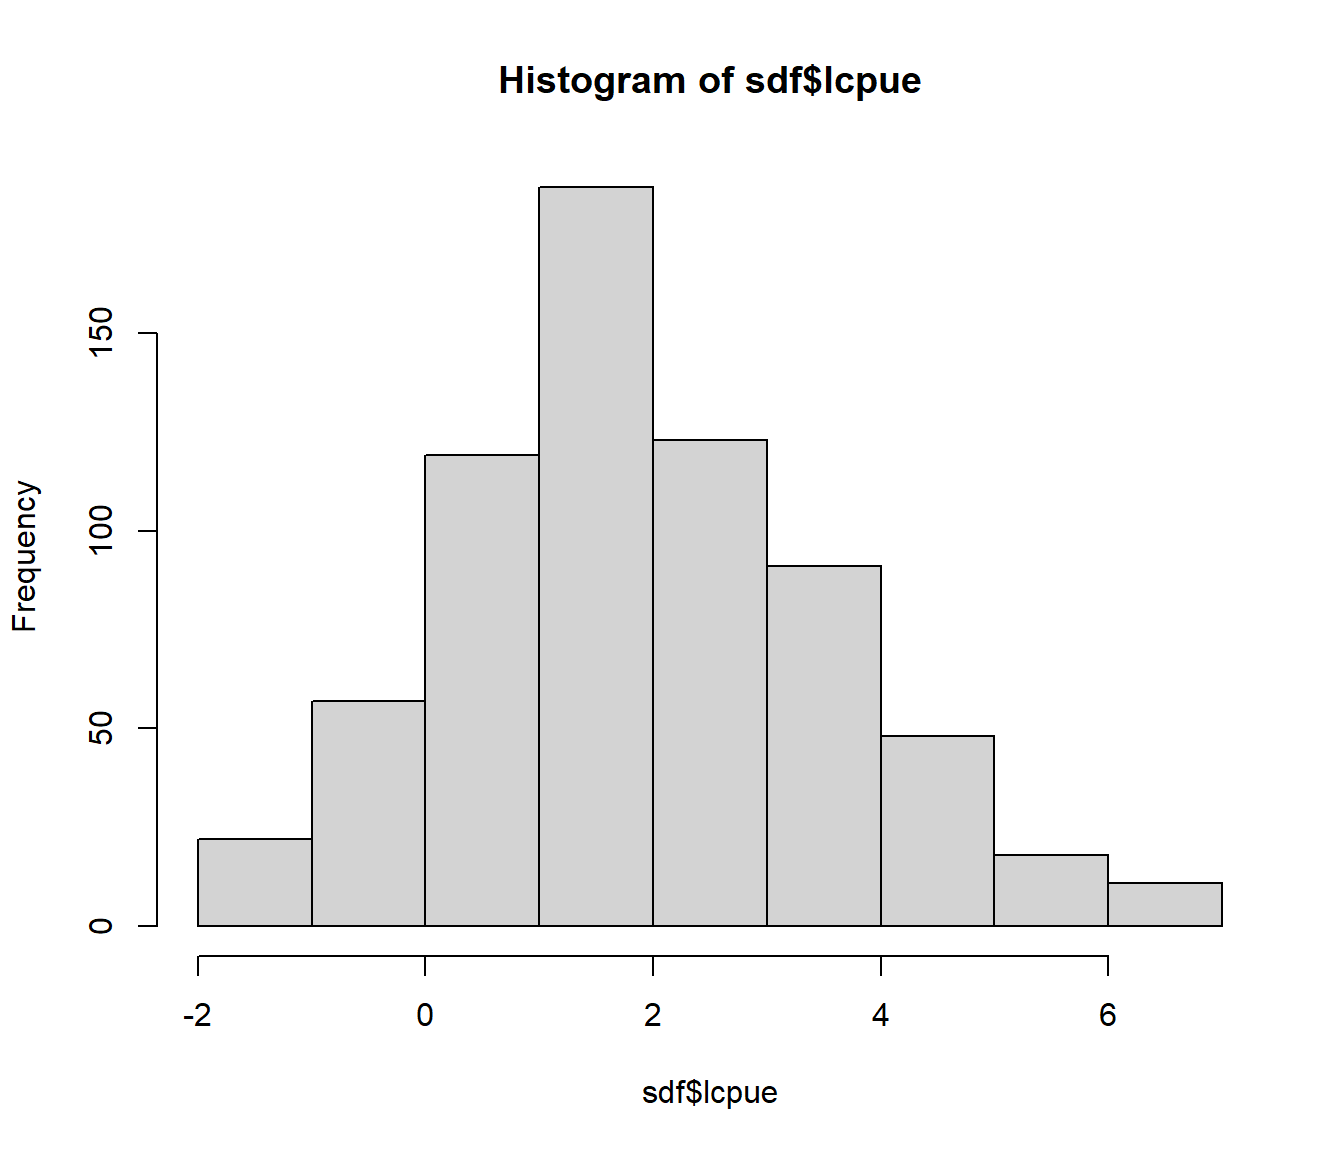
\includegraphics[width=0.7\linewidth]{11-sp_files/figure-latex/unnamed-chunk-11-2} \end{center}

\begin{Shaded}
\begin{Highlighting}[]
\FunctionTok{spplot}\NormalTok{(sdf, }\StringTok{"lcpue"}\NormalTok{)}
\end{Highlighting}
\end{Shaded}

\begin{center}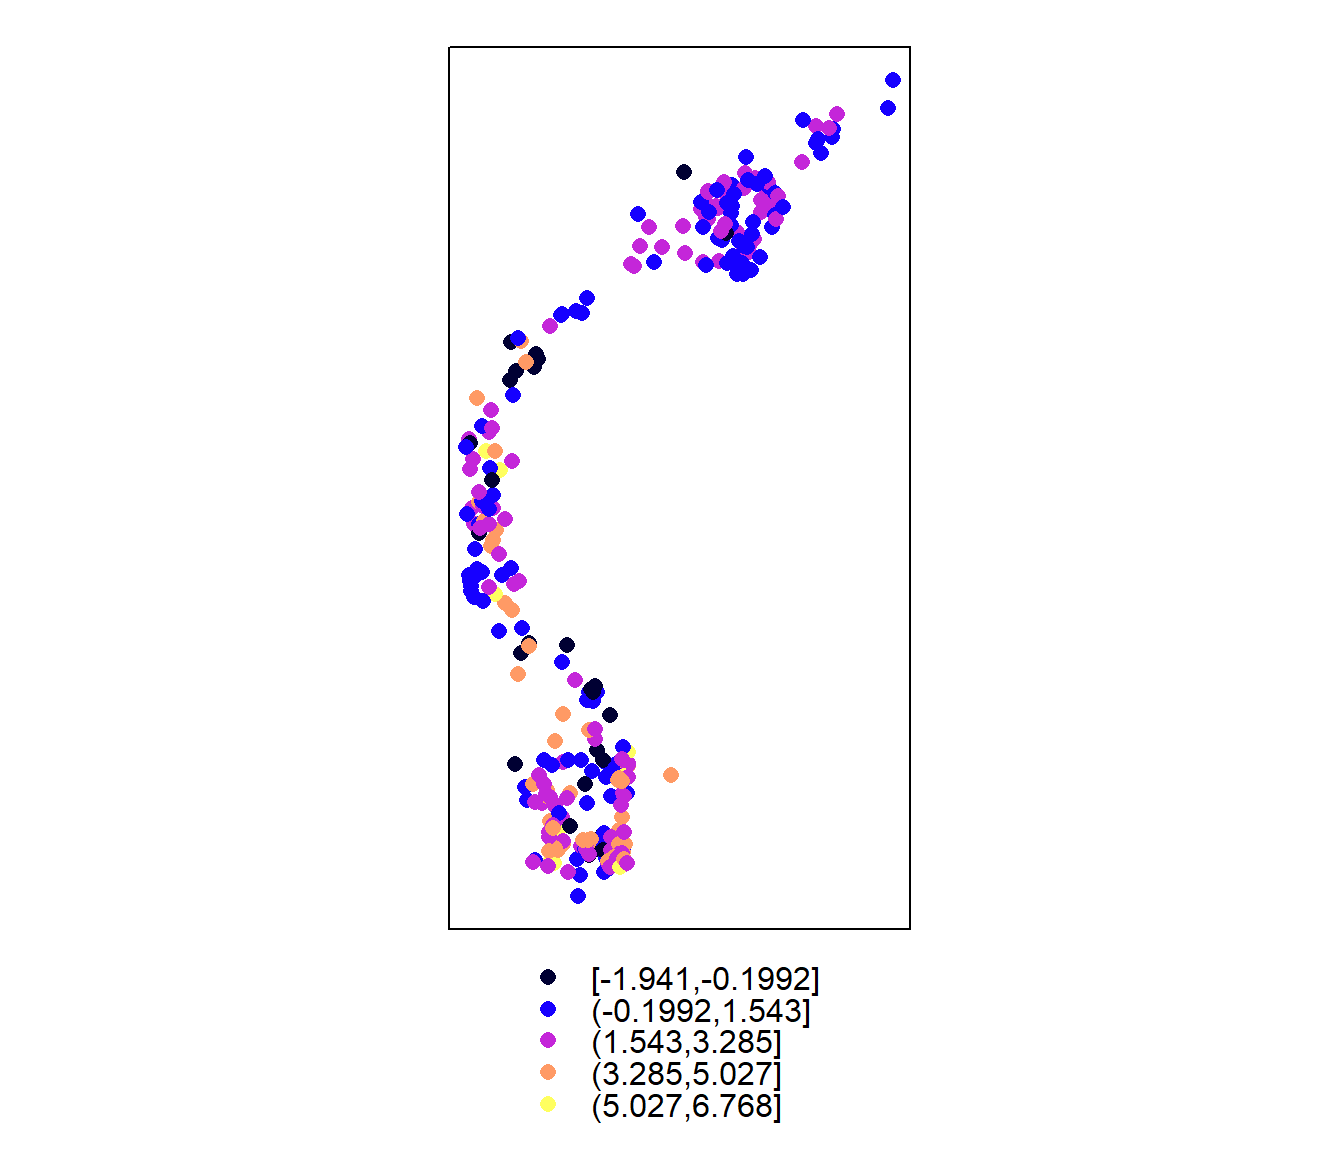
\includegraphics[width=0.7\linewidth]{11-sp_files/figure-latex/unnamed-chunk-11-3} \end{center}

\hypertarget{spatiallines-y-spatialpolygons}{%
\subsection{SpatialLines y SpatialPolygons}\label{spatiallines-y-spatialpolygons}}

\begin{itemize}
\item
  Tipo \texttt{SpatialLines}

  \begin{itemize}
  \item
    Basados en \texttt{Line}: \texttt{coords}
  \item
    Se combinan objetos \texttt{Line} en listas: \texttt{lines,\ bbox,\ proj4string}
  \item
    De utilidad principalmente para representaciones gráficas (y
    para generar polígonos).
  \end{itemize}
\item
  Tipo \texttt{SpatialPolygons}

  \begin{itemize}
  \item
    Basados en \texttt{Polygon}:
    \texttt{labpt,\ area,\ hole,\ ringDir,\ coords}(extiende \texttt{Line} de forma
    que la primera y la última línea es la misma)\texttt{.}
  \item
    Se combinan objetos \texttt{Polygon} en listas:
    \texttt{polygons,\ plotOrder,\ bbox,\ proj4string.}
  \item
    De utilidad principalmente para representaciones gráficas (y
    \texttt{overlay}).
  \end{itemize}
\item
  Se extienden también a \texttt{Spatial*DataFrame} (slot \texttt{data})

  \begin{itemize}
  \tightlist
  \item
    \texttt{SpatialPolygonsDataFrame}: util para procesos reticulares.
  \end{itemize}
\end{itemize}

\hypertarget{ejemplo-spatiallines}{%
\subsubsection{Ejemplo SpatialLines}\label{ejemplo-spatiallines}}

El fichero \emph{costa.galicia.txt} contiene la costa de Galicia en formato Mapgen.
Descargada del (difunto) \href{http://www.ngdc.noaa.gov/mgg/shorelines/shorelines.html}{Coastline Extractor}

\begin{Shaded}
\begin{Highlighting}[]
\FunctionTok{library}\NormalTok{(maptools) }\CommentTok{\# Utilidades para convertir datos entre diferentes formatos espaciales}
\end{Highlighting}
\end{Shaded}

\begin{verbatim}
## Checking rgeos availability: TRUE
\end{verbatim}

\begin{Shaded}
\begin{Highlighting}[]
\NormalTok{costa.galicia }\OtherTok{\textless{}{-}} \FunctionTok{MapGen2SL}\NormalTok{(}\StringTok{"datos/costa.galicia.txt"}\NormalTok{, }\FunctionTok{CRS}\NormalTok{(}\StringTok{"+proj=longlat +ellps=WGS84"}\NormalTok{))}

\FunctionTok{summary}\NormalTok{(costa.galicia)}
\end{Highlighting}
\end{Shaded}

\begin{verbatim}
## Object of class SpatialLines
## Coordinates:
##         min       max
## x -9.305495 -6.500147
## y 41.500846 43.791944
## Is projected: FALSE 
## proj4string : [+proj=longlat +ellps=WGS84 +no_defs]
\end{verbatim}

\begin{Shaded}
\begin{Highlighting}[]
\FunctionTok{plot}\NormalTok{(sdf, }\AttributeTok{axes=}\ConstantTok{TRUE}\NormalTok{)}
\FunctionTok{plot}\NormalTok{(costa.galicia, }\AttributeTok{add=}\ConstantTok{TRUE}\NormalTok{)}
\end{Highlighting}
\end{Shaded}

\begin{center}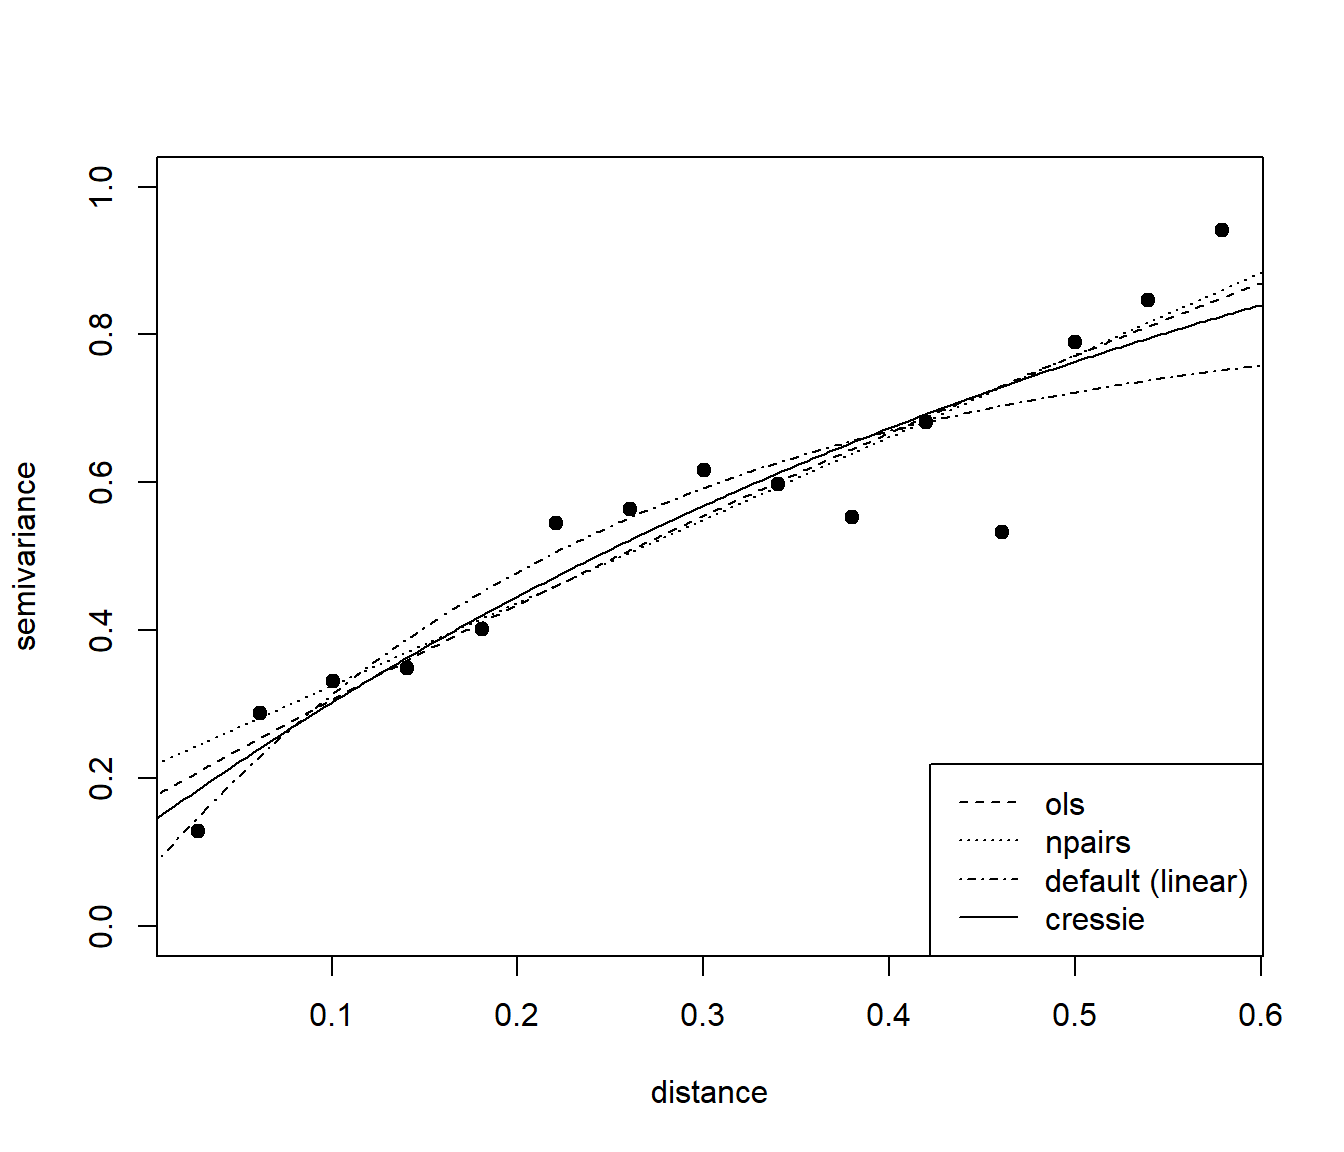
\includegraphics[width=0.7\linewidth]{11-sp_files/figure-latex/unnamed-chunk-12-1} \end{center}

\hypertarget{ejemplo-spatialpolygonsdataframe}{%
\subsubsection{Ejemplo SpatialPolygonsDataFrame}\label{ejemplo-spatialpolygonsdataframe}}

Los objetos de este tipo se suelen crear a partir de objetos \texttt{SpatialLines},
pero hay que asegurarse de que definen adecuadamente un polígono.

Objetos de este tipo se pueden descargar de
\href{http://www.gadm.org}{GADM database of Global Administrative Areas}.
Contienen límites administrativos a disintos niveles, e.g.:

\begin{itemize}
\item
  \texttt{ESP\_adm0.rds} límites España e islas
\item
  \texttt{ESP\_adm1.rds} límites Autonomías
\item
  \texttt{ESP\_adm2.rds} límites Provincias
\item
  \texttt{ESP\_adm3.rds} límites Comarcas
\item
  \texttt{ESP\_adm4.rds} límites Ayuntamientos
\end{itemize}

NOTA: Se podrían descargar directamente desde R, e.g.:

\begin{verbatim}
  con <- url('http://gadm.org/data/rda/ESP_adm1.rds')
  gadm <- readRDS(con)
  close(con)
\end{verbatim}

Carga de un objeto gadm:

\begin{Shaded}
\begin{Highlighting}[]
\NormalTok{gadm }\OtherTok{\textless{}{-}} \FunctionTok{readRDS}\NormalTok{(}\StringTok{"datos/ESP\_adm1.rds"}\NormalTok{) }
\FunctionTok{summary}\NormalTok{(gadm)}
\end{Highlighting}
\end{Shaded}

\begin{verbatim}
## Object of class SpatialPolygonsDataFrame
## Coordinates:
##         min       max
## x -18.16153  4.328195
## y  27.63736 43.791527
## Is projected: FALSE 
## proj4string :
## [+proj=longlat +datum=WGS84 +no_defs +ellps=WGS84 +towgs84=0,0,0]
## Data attributes:
##     OBJECTID          ID_0         ISO               NAME_0         
##  Min.   : 1.00   Min.   :215   Length:18          Length:18         
##  1st Qu.: 5.25   1st Qu.:215   Class :character   Class :character  
##  Median : 9.50   Median :215   Mode  :character   Mode  :character  
##  Mean   : 9.50   Mean   :215                                        
##  3rd Qu.:13.75   3rd Qu.:215                                        
##  Max.   :18.00   Max.   :215                                        
##                                                                     
##       ID_1          NAME_1             HASC_1              CCN_1    
##  Min.   : 1.00   Length:18          Length:18          Min.   : NA  
##  1st Qu.: 5.25   Class :character   Class :character   1st Qu.: NA  
##  Median : 9.50   Mode  :character   Mode  :character   Median : NA  
##  Mean   : 9.50                                         Mean   :NaN  
##  3rd Qu.:13.75                                         3rd Qu.: NA  
##  Max.   :18.00                                         Max.   : NA  
##                                                        NA's   :18   
##     CCA_1              TYPE_1           ENGTYPE_1          NL_NAME_1        
##  Length:18          Length:18          Length:18          Length:18         
##  Class :character   Class :character   Class :character   Class :character  
##  Mode  :character   Mode  :character   Mode  :character   Mode  :character  
##                                                                             
##                                                                             
##                                                                             
##                                                                             
##   VARNAME_1        
##  Length:18         
##  Class :character  
##  Mode  :character  
##                    
##                    
##                    
## 
\end{verbatim}

\begin{Shaded}
\begin{Highlighting}[]
\FunctionTok{plot}\NormalTok{(gadm)}
\end{Highlighting}
\end{Shaded}

\begin{center}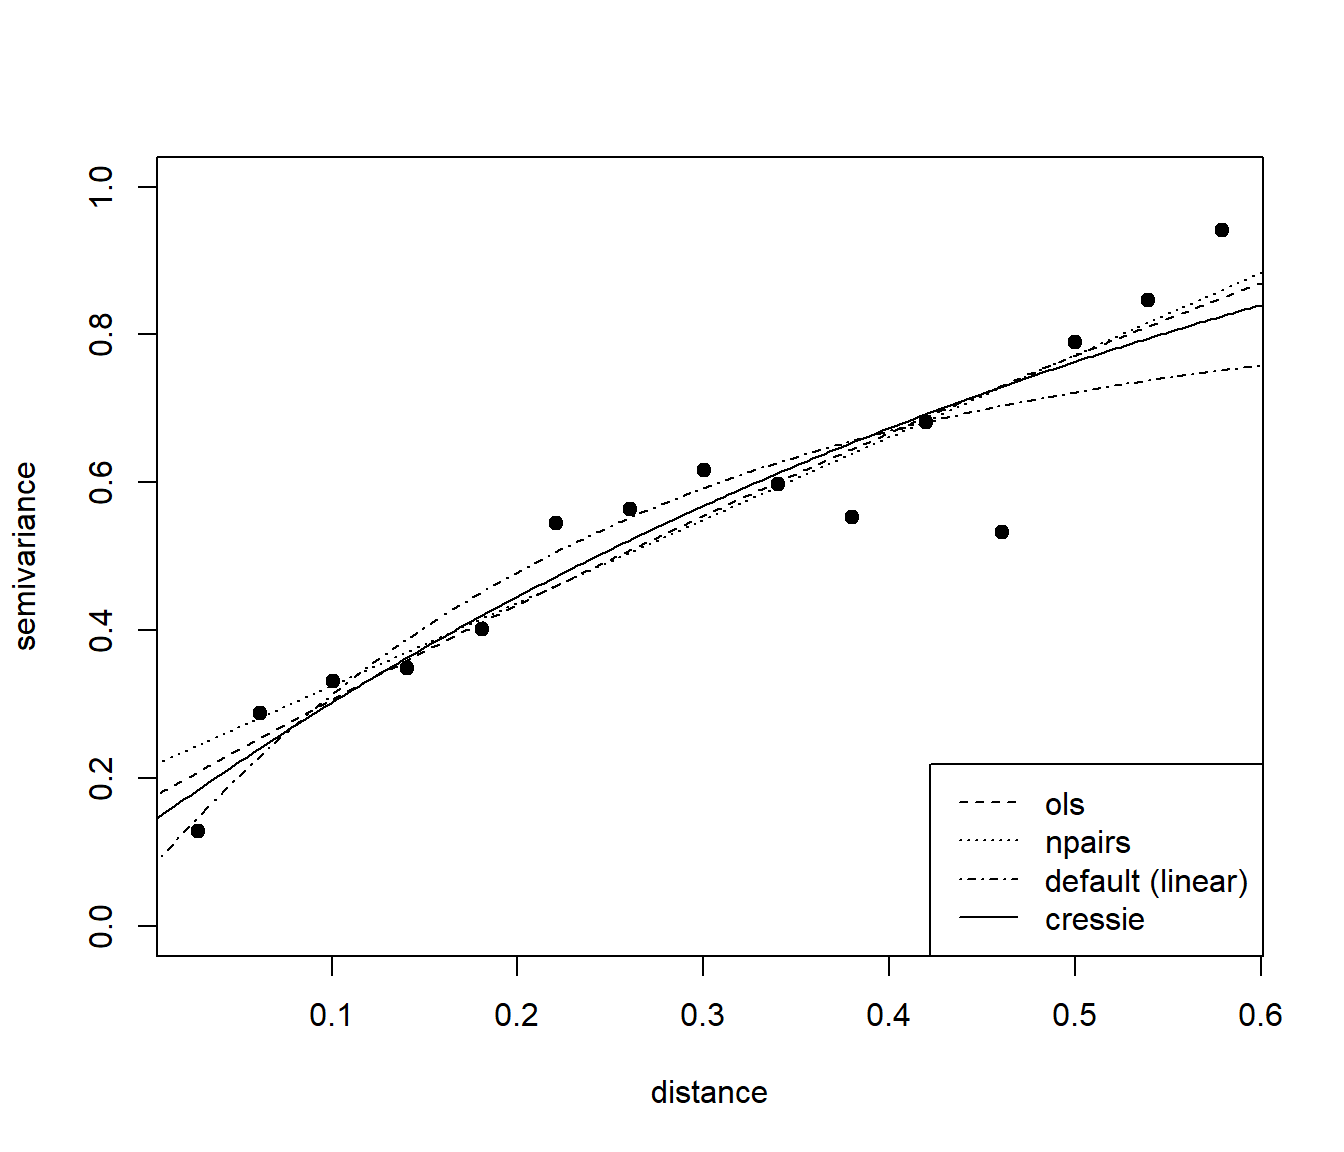
\includegraphics[width=0.7\linewidth]{11-sp_files/figure-latex/unnamed-chunk-13-1} \end{center}

\begin{Shaded}
\begin{Highlighting}[]
\CommentTok{\# Cuidado objeto muy grande: str(gadm)}
\CommentTok{\# Mejor emplear str(gadm, 3)}
\end{Highlighting}
\end{Shaded}

Extraer autonomía de Galicia:

\begin{Shaded}
\begin{Highlighting}[]
\FunctionTok{names}\NormalTok{(gadm)}
\end{Highlighting}
\end{Shaded}

\begin{verbatim}
##  [1] "OBJECTID"  "ID_0"      "ISO"       "NAME_0"    "ID_1"      "NAME_1"   
##  [7] "HASC_1"    "CCN_1"     "CCA_1"     "TYPE_1"    "ENGTYPE_1" "NL_NAME_1"
## [13] "VARNAME_1"
\end{verbatim}

\begin{Shaded}
\begin{Highlighting}[]
\NormalTok{galicia }\OtherTok{\textless{}{-}}\NormalTok{ gadm[gadm}\SpecialCharTok{$}\NormalTok{NAME\_1 }\SpecialCharTok{==} \StringTok{"Galicia"}\NormalTok{, ]}
\FunctionTok{plot}\NormalTok{(galicia)}
\end{Highlighting}
\end{Shaded}

\begin{center}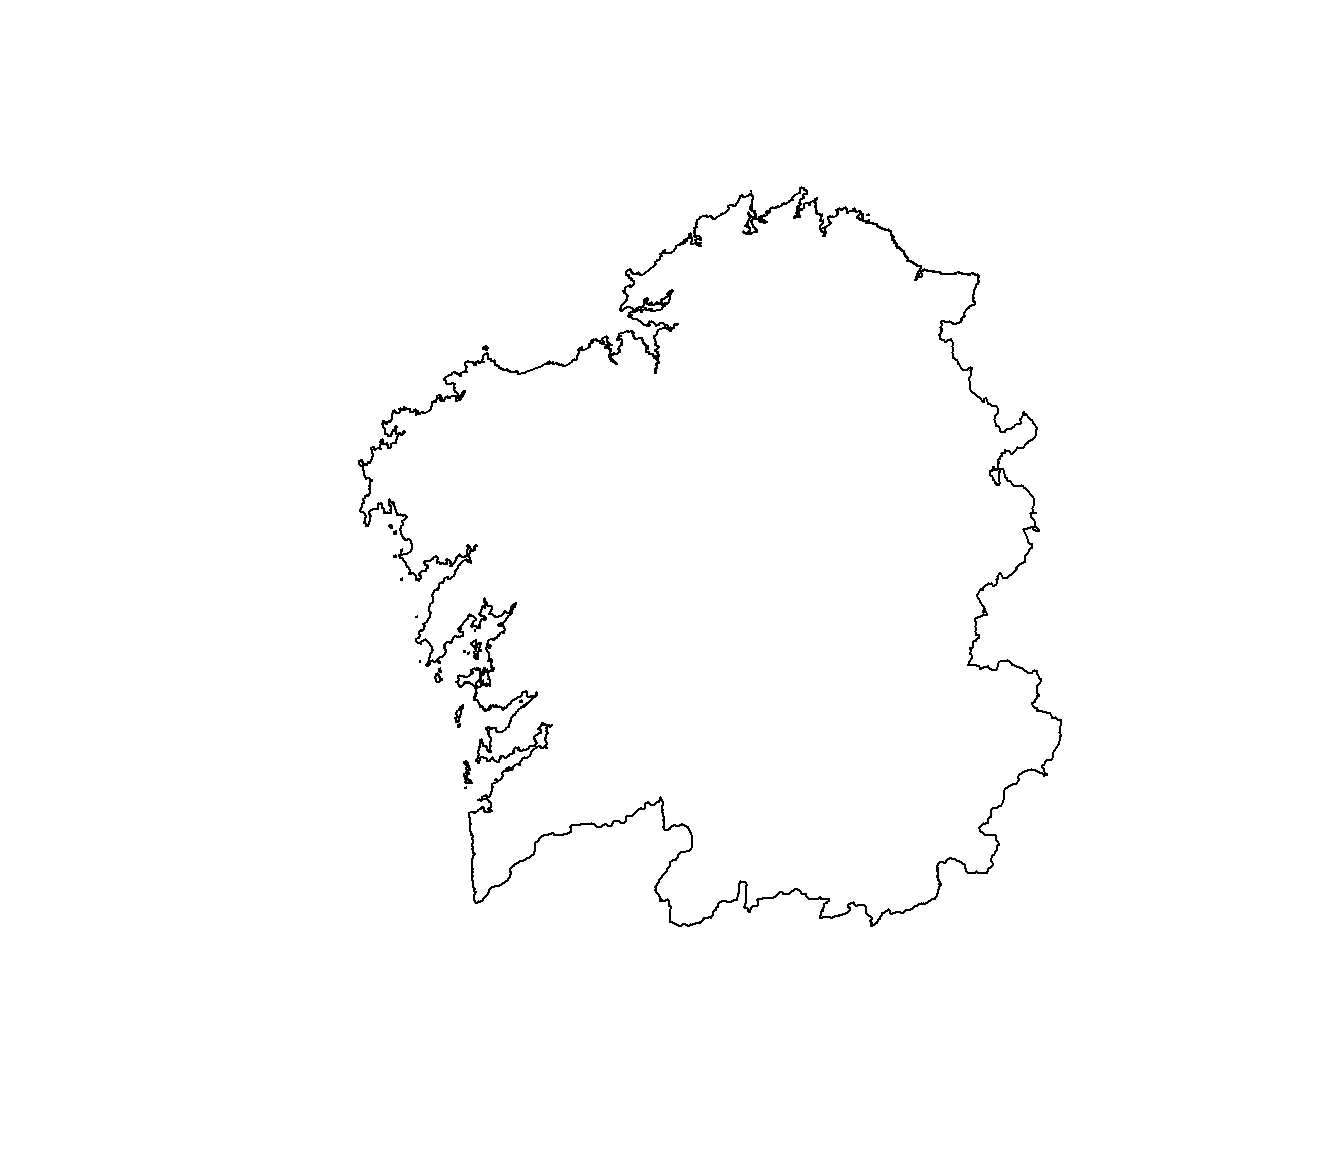
\includegraphics[width=0.7\linewidth]{11-sp_files/figure-latex/unnamed-chunk-14-1} \end{center}

Es preferible emplear este tipo de objetos a \texttt{SpatialLines}:

\begin{Shaded}
\begin{Highlighting}[]
\FunctionTok{plot}\NormalTok{(sdf, }\AttributeTok{axes=}\ConstantTok{TRUE}\NormalTok{)}
\FunctionTok{plot}\NormalTok{(galicia, }\AttributeTok{add=}\ConstantTok{TRUE}\NormalTok{)}
\end{Highlighting}
\end{Shaded}

\begin{center}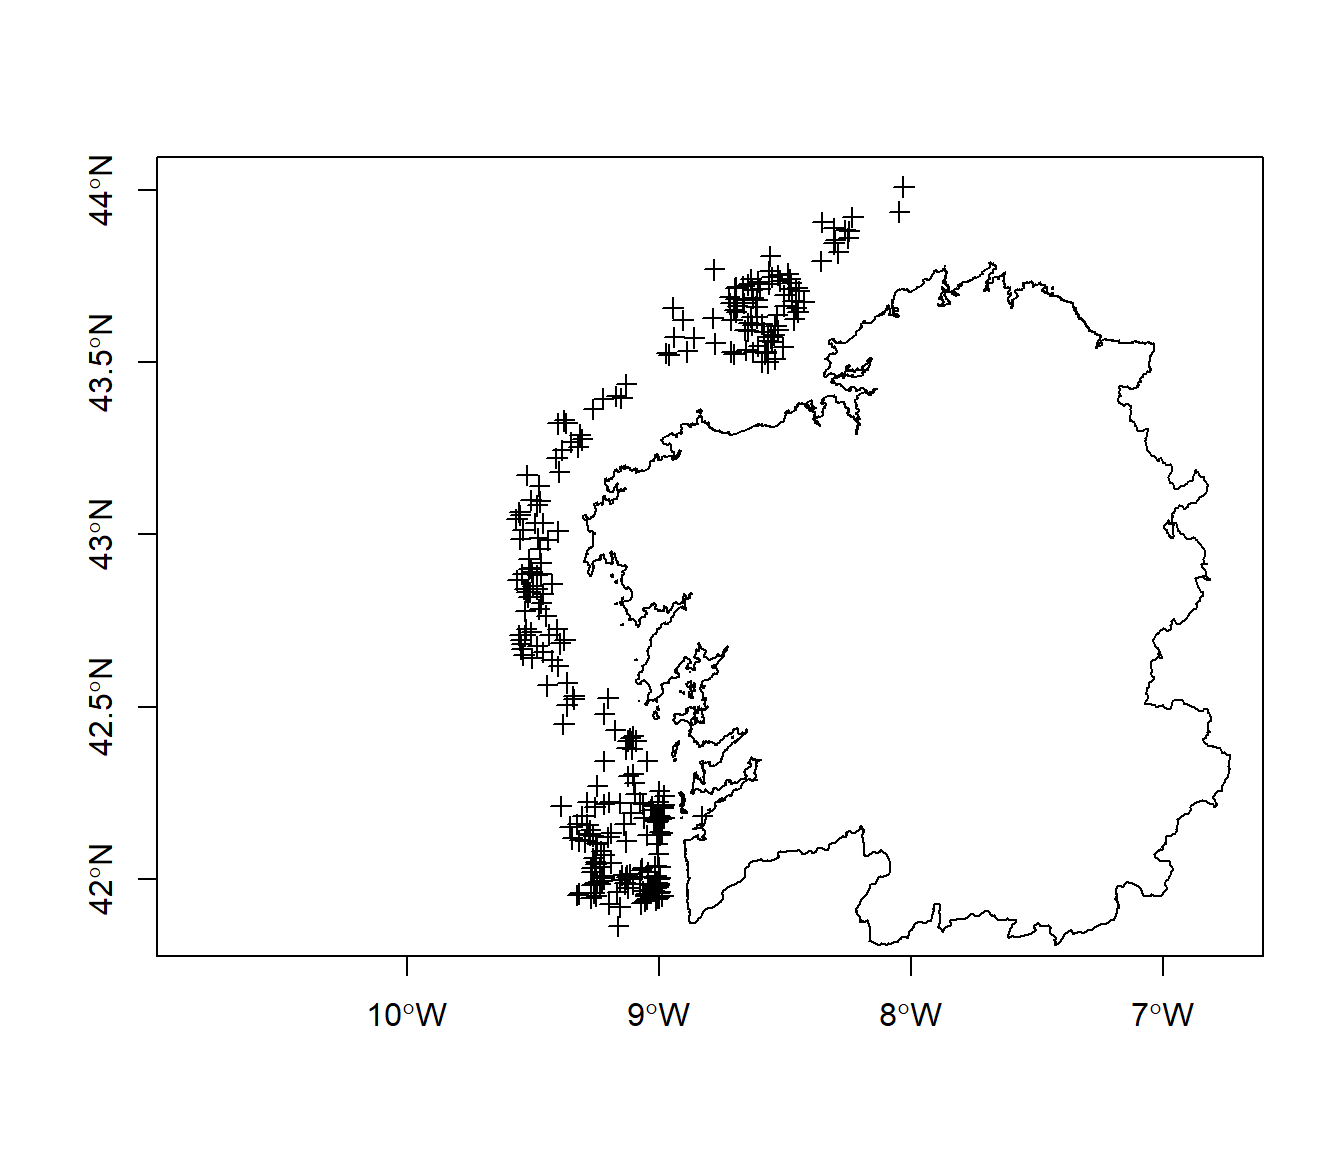
\includegraphics[width=0.7\linewidth]{11-sp_files/figure-latex/unnamed-chunk-15-1} \end{center}

\hypertarget{spatialgrid-y-spatialpixels}{%
\subsection{SpatialGrid y SpatialPixels}\label{spatialgrid-y-spatialpixels}}

Es habitual trabajar con datos espaciales en formato
rejilla (grid) (e.g.~predicciones en geoestadística):

\begin{itemize}
\item
  Rejilla (posiciones) definida por un objeto \texttt{GridTopology}:
  \texttt{cellcentre.offset,\ cellsize,\ cells.dim}
\item
  Tipos \texttt{SpatialGrid} y \texttt{SpatialPixels}:
  \texttt{grid,\ grid.index,\ coords,\ bbox,\ proj4string}
\item
  Se extienden también a \texttt{Spatial*DataFrame} (slot \texttt{data})
\item
  Los objetos \texttt{SpatialGrid} se corresponden con la rejilla completa:
\item
  Los objetos \texttt{SpatialPixels} se corresponden con una rejilla
  incompleta

  \begin{itemize}
  \item
    \texttt{coords}contiene todas las coordenadas (objetos equivalentes a
    \texttt{SpatialPoints})
  \item
    \texttt{grid.index}indices de la rejilla
  \end{itemize}
\end{itemize}

\hypertarget{ejemplo-spatialgrid}{%
\subsubsection{Ejemplo SpatialGrid}\label{ejemplo-spatialgrid}}

Importante si se utiliza el paquete \texttt{gstat}\ldots{}

\begin{Shaded}
\begin{Highlighting}[]
\NormalTok{xrange }\OtherTok{\textless{}{-}} \FunctionTok{c}\NormalTok{(}\SpecialCharTok{{-}}\DecValTok{10}\NormalTok{, }\SpecialCharTok{{-}}\FloatTok{7.5}\NormalTok{)}
\NormalTok{yrange }\OtherTok{\textless{}{-}} \FunctionTok{c}\NormalTok{(}\FloatTok{42.25}\NormalTok{, }\DecValTok{44}\NormalTok{)}
\NormalTok{nx }\OtherTok{\textless{}{-}} \DecValTok{100}
\NormalTok{ny }\OtherTok{\textless{}{-}} \DecValTok{100}
\NormalTok{hx }\OtherTok{\textless{}{-}} \FunctionTok{diff}\NormalTok{(xrange)}\SpecialCharTok{/}\NormalTok{(nx}\DecValTok{{-}1}\NormalTok{)}
\NormalTok{hy }\OtherTok{\textless{}{-}} \FunctionTok{diff}\NormalTok{(yrange)}\SpecialCharTok{/}\NormalTok{(ny}\DecValTok{{-}1}\NormalTok{)}

\NormalTok{gridtop }\OtherTok{\textless{}{-}} \FunctionTok{GridTopology}\NormalTok{(}\AttributeTok{cellcentre.offset =} \FunctionTok{c}\NormalTok{(}\FunctionTok{min}\NormalTok{(xrange), }\FunctionTok{min}\NormalTok{(yrange)),}
                        \AttributeTok{cellsize =} \FunctionTok{c}\NormalTok{(hx, hy), }\AttributeTok{cells.dim =} \FunctionTok{c}\NormalTok{(nx, ny))}
\NormalTok{spgrid }\OtherTok{\textless{}{-}}  \FunctionTok{SpatialGrid}\NormalTok{(gridtop, }\AttributeTok{proj4string =} \FunctionTok{proj4string}\NormalTok{(gadm))}

\FunctionTok{str}\NormalTok{(spgrid)}
\end{Highlighting}
\end{Shaded}

\begin{verbatim}
## Formal class 'SpatialGrid' [package "sp"] with 3 slots
##   ..@ grid       :Formal class 'GridTopology' [package "sp"] with 3 slots
##   .. .. ..@ cellcentre.offset: num [1:2] -10 42.2
##   .. .. ..@ cellsize         : num [1:2] 0.0253 0.0177
##   .. .. ..@ cells.dim        : int [1:2] 100 100
##   ..@ bbox       : num [1:2, 1:2] -10.01 42.24 -7.49 44.01
##   .. ..- attr(*, "dimnames")=List of 2
##   .. .. ..$ : NULL
##   .. .. ..$ : chr [1:2] "min" "max"
##   ..@ proj4string:Formal class 'CRS' [package "sp"] with 1 slot
##   .. .. ..@ projargs: chr "+proj=longlat +datum=WGS84 +no_defs"
##   .. .. ..$ comment: chr "GEOGCRS[\"unknown\",\n    DATUM[\"World Geodetic System 1984\",\n        ELLIPSOID[\"WGS 84\",6378137,298.25722"| __truncated__
\end{verbatim}

\begin{Shaded}
\begin{Highlighting}[]
\FunctionTok{plot}\NormalTok{(spgrid, }\AttributeTok{axes =} \ConstantTok{TRUE}\NormalTok{)}
\FunctionTok{plot}\NormalTok{(galicia, }\AttributeTok{add =} \ConstantTok{TRUE}\NormalTok{)}
\end{Highlighting}
\end{Shaded}

\begin{center}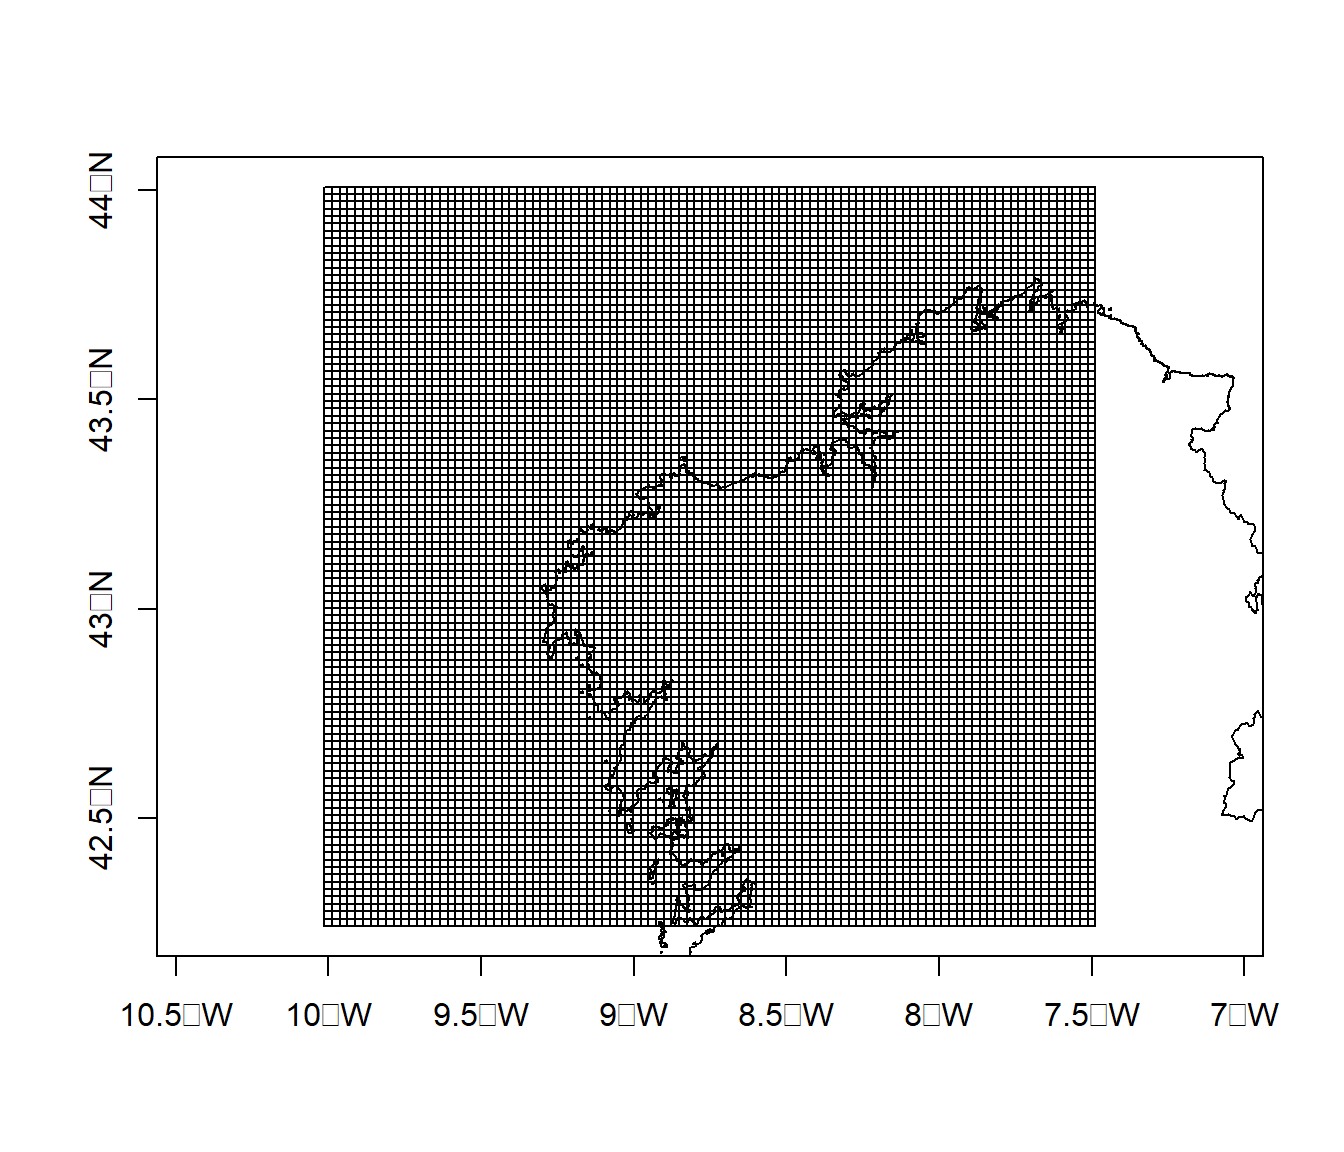
\includegraphics[width=0.7\linewidth]{11-sp_files/figure-latex/unnamed-chunk-16-1} \end{center}

\hypertarget{ejemplo-spatialpixels}{%
\subsubsection{Ejemplo SpatialPixels}\label{ejemplo-spatialpixels}}

\begin{Shaded}
\begin{Highlighting}[]
\CommentTok{\# over: combinación de objetos espaciales}
\NormalTok{index }\OtherTok{\textless{}{-}} \FunctionTok{over}\NormalTok{(spgrid, }\FunctionTok{as}\NormalTok{(galicia, }\StringTok{"SpatialPolygons"}\NormalTok{))}
\NormalTok{sppix }\OtherTok{\textless{}{-}} \FunctionTok{as}\NormalTok{(spgrid, }\StringTok{"SpatialPixels"}\NormalTok{)[}\FunctionTok{is.na}\NormalTok{(index), ]}

\FunctionTok{str}\NormalTok{(sppix)}
\end{Highlighting}
\end{Shaded}

\begin{verbatim}
## Formal class 'SpatialPixels' [package "sp"] with 5 slots
##   ..@ grid       :Formal class 'GridTopology' [package "sp"] with 3 slots
##   .. .. ..@ cellcentre.offset: num [1:2] -10 42.2
##   .. .. ..@ cellsize         : num [1:2] 0.0253 0.0177
##   .. .. ..@ cells.dim        : int [1:2] 100 100
##   ..@ grid.index : int [1:5631] 1 2 3 4 5 6 7 8 9 10 ...
##   ..@ coords     : num [1:5631, 1:2] -10 -9.97 -9.95 -9.92 -9.9 ...
##   .. ..- attr(*, "dimnames")=List of 2
##   .. .. ..$ : NULL
##   .. .. ..$ : chr [1:2] "s1" "s2"
##   ..@ bbox       : num [1:2, 1:2] -10.01 42.24 -7.49 44.01
##   .. ..- attr(*, "dimnames")=List of 2
##   .. .. ..$ : chr [1:2] "s1" "s2"
##   .. .. ..$ : chr [1:2] "min" "max"
##   ..@ proj4string:Formal class 'CRS' [package "sp"] with 1 slot
##   .. .. ..@ projargs: chr "+proj=longlat +datum=WGS84 +no_defs"
##   .. .. ..$ comment: chr "GEOGCRS[\"unknown\",\n    DATUM[\"World Geodetic System 1984\",\n        ELLIPSOID[\"WGS 84\",6378137,298.25722"| __truncated__
\end{verbatim}

\begin{Shaded}
\begin{Highlighting}[]
\FunctionTok{plot}\NormalTok{(sppix, }\AttributeTok{axes =} \ConstantTok{TRUE}\NormalTok{)}
\FunctionTok{plot}\NormalTok{(galicia, }\AttributeTok{add =} \ConstantTok{TRUE}\NormalTok{)}
\end{Highlighting}
\end{Shaded}

\begin{center}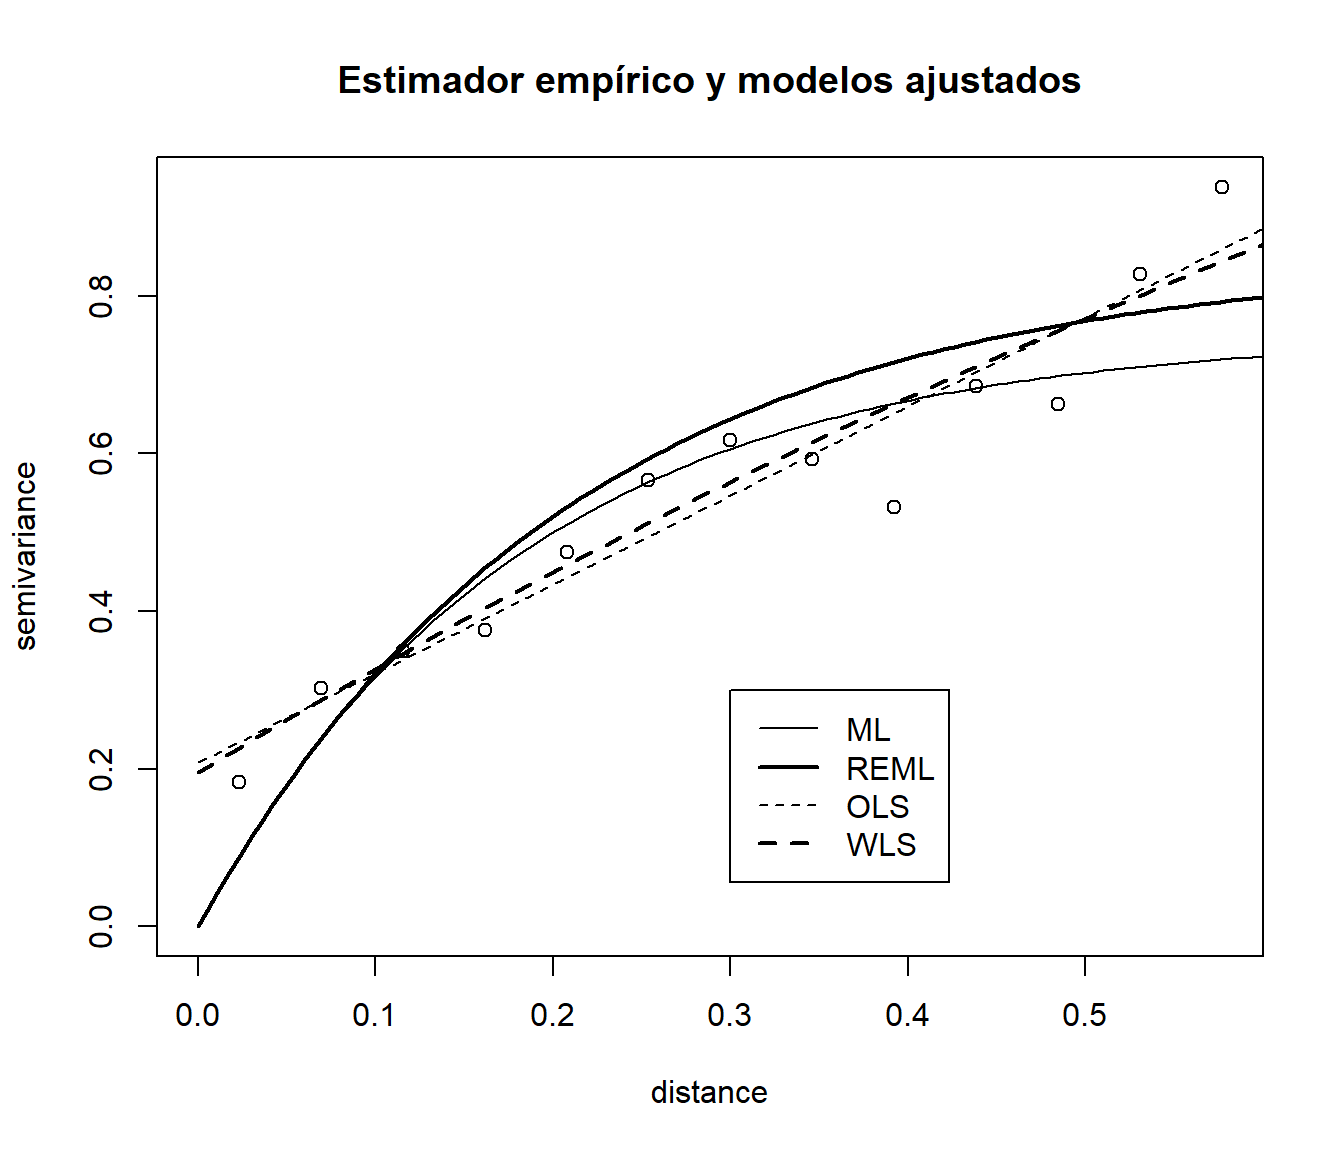
\includegraphics[width=0.7\linewidth]{11-sp_files/figure-latex/unnamed-chunk-17-1} \end{center}

\begin{Shaded}
\begin{Highlighting}[]
\CommentTok{\# NOTA: puede ser preferible asignar NA\textquotesingle{}s a variables en SpatialGridDataFrame...}
\FunctionTok{object.size}\NormalTok{(spgrid)}
\end{Highlighting}
\end{Shaded}

\begin{verbatim}
## 4040 bytes
\end{verbatim}

\begin{Shaded}
\begin{Highlighting}[]
\FunctionTok{object.size}\NormalTok{(sppix)}
\end{Highlighting}
\end{Shaded}

\begin{verbatim}
## 117680 bytes
\end{verbatim}

\begin{Shaded}
\begin{Highlighting}[]
\CommentTok{\# Otras funciones:}
\CommentTok{\# as(sppix, "SpatialGrid") recostruye la rejilla completa}
\CommentTok{\# gridded(ObjetoSpatialPoints) \textless{}{-} TRUE  convierte el objeto SpatialPoints en SpatialPixels}
\end{Highlighting}
\end{Shaded}

\hypertarget{muxe9todos-y-procedimientos-clases-sp}{%
\section{Métodos y procedimientos clases sp}\label{muxe9todos-y-procedimientos-clases-sp}}

\begin{longtable}[]{@{}
  >{\raggedright\arraybackslash}p{(\columnwidth - 2\tabcolsep) * \real{0.13}}
  >{\raggedright\arraybackslash}p{(\columnwidth - 2\tabcolsep) * \real{0.87}}@{}}
\toprule
Método & Descripción \\
\midrule
\endhead
\texttt{{[}} & selecciona elementos espaciales (puntos, líneas, polígonos, filas/columnas de una rejilla) y/o variables. \\
\texttt{\$,\ {[}{[}} & obtiene, establece o agrega variables (columnas). \\
\texttt{coordinates} & obtiene o establece (creando objetos sp) coordenadas. \\
\texttt{as(obj,\ clase)} & convierte un objeto a una clase. \\
\texttt{over,\ overlay} & combina objetos espaciales. \\
\texttt{spsample} & muestrea puntos dentro de una región (rectangular, polígono, línea o rejilla). \\
\bottomrule
\end{longtable}

\hypertarget{importarexportartransformar}{%
\subsection{Importar/exportar/transformar}\label{importarexportartransformar}}

A través de R (paquetes que emplean sp) es fácil exportar datos a otras aplicaciones
(e.g.~\href{http://plotkml.r-forge.r-project.org}{Google Earth}).

Ejemplo importación:

Datos descargados en formato NetCDF (\href{http://www.opengeospatial.org/standards/netcdf}{Network Common Data Form})
de \href{http://www.esrl.noaa.gov/psd/data/gridded/data.noaa.oisst.v2.html}{NOAA Optimum Interpolated Sea Surface Temperature V2 (OISST)}
y procesados con \emph{\href{datos/NOAA_OISST_extraction_v2.R}{NOAA\_OISST\_extraction\_v2.R}}:

\begin{Shaded}
\begin{Highlighting}[]
\FunctionTok{load}\NormalTok{(}\StringTok{"datos/sstsp.RData"}\NormalTok{) }\CommentTok{\# SST 15{-}04{-}2012 }
\NormalTok{jet.colors }\OtherTok{\textless{}{-}} \FunctionTok{colorRampPalette}\NormalTok{(}\FunctionTok{c}\NormalTok{(}\StringTok{"\#00007F"}\NormalTok{, }\StringTok{"blue"}\NormalTok{, }\StringTok{"\#007FFF"}\NormalTok{, }\StringTok{"cyan"}\NormalTok{, }\StringTok{"\#7FFF7F"}\NormalTok{, }\StringTok{"yellow"}\NormalTok{, }\StringTok{"\#FF7F00"}\NormalTok{, }\StringTok{"red"}\NormalTok{, }\StringTok{"\#7F0000"}\NormalTok{))}
\FunctionTok{image}\NormalTok{(sstsp, }\AttributeTok{col =} \FunctionTok{jet.colors}\NormalTok{(}\DecValTok{128}\NormalTok{), }\AttributeTok{axes =} \ConstantTok{TRUE}\NormalTok{)}
\FunctionTok{title}\NormalTok{(}\FunctionTok{attr}\NormalTok{(sstsp}\SpecialCharTok{@}\NormalTok{data, }\StringTok{"label"}\NormalTok{))}

\CommentTok{\# Ejemplo importar datos de otros paquetes:}
\FunctionTok{library}\NormalTok{(maps)}
\FunctionTok{library}\NormalTok{(maptools)}
\NormalTok{world }\OtherTok{\textless{}{-}} \FunctionTok{map}\NormalTok{(}\StringTok{"world"}\NormalTok{, }\AttributeTok{fill =} \ConstantTok{TRUE}\NormalTok{, }\AttributeTok{plot =} \ConstantTok{FALSE}\NormalTok{)   }\CommentTok{\# Hay un mapa con mayor resolución en mapdata::worldHires}
\NormalTok{world\_pol }\OtherTok{\textless{}{-}} \FunctionTok{map2SpatialPolygons}\NormalTok{(world, world}\SpecialCharTok{$}\NormalTok{names, }\FunctionTok{CRS}\NormalTok{(}\StringTok{"+proj=longlat +ellps=WGS84"}\NormalTok{))}
\FunctionTok{plot}\NormalTok{(world\_pol, }\AttributeTok{col =} \StringTok{\textquotesingle{}white\textquotesingle{}}\NormalTok{, }\AttributeTok{add =} \ConstantTok{TRUE}\NormalTok{) }
\end{Highlighting}
\end{Shaded}

\begin{center}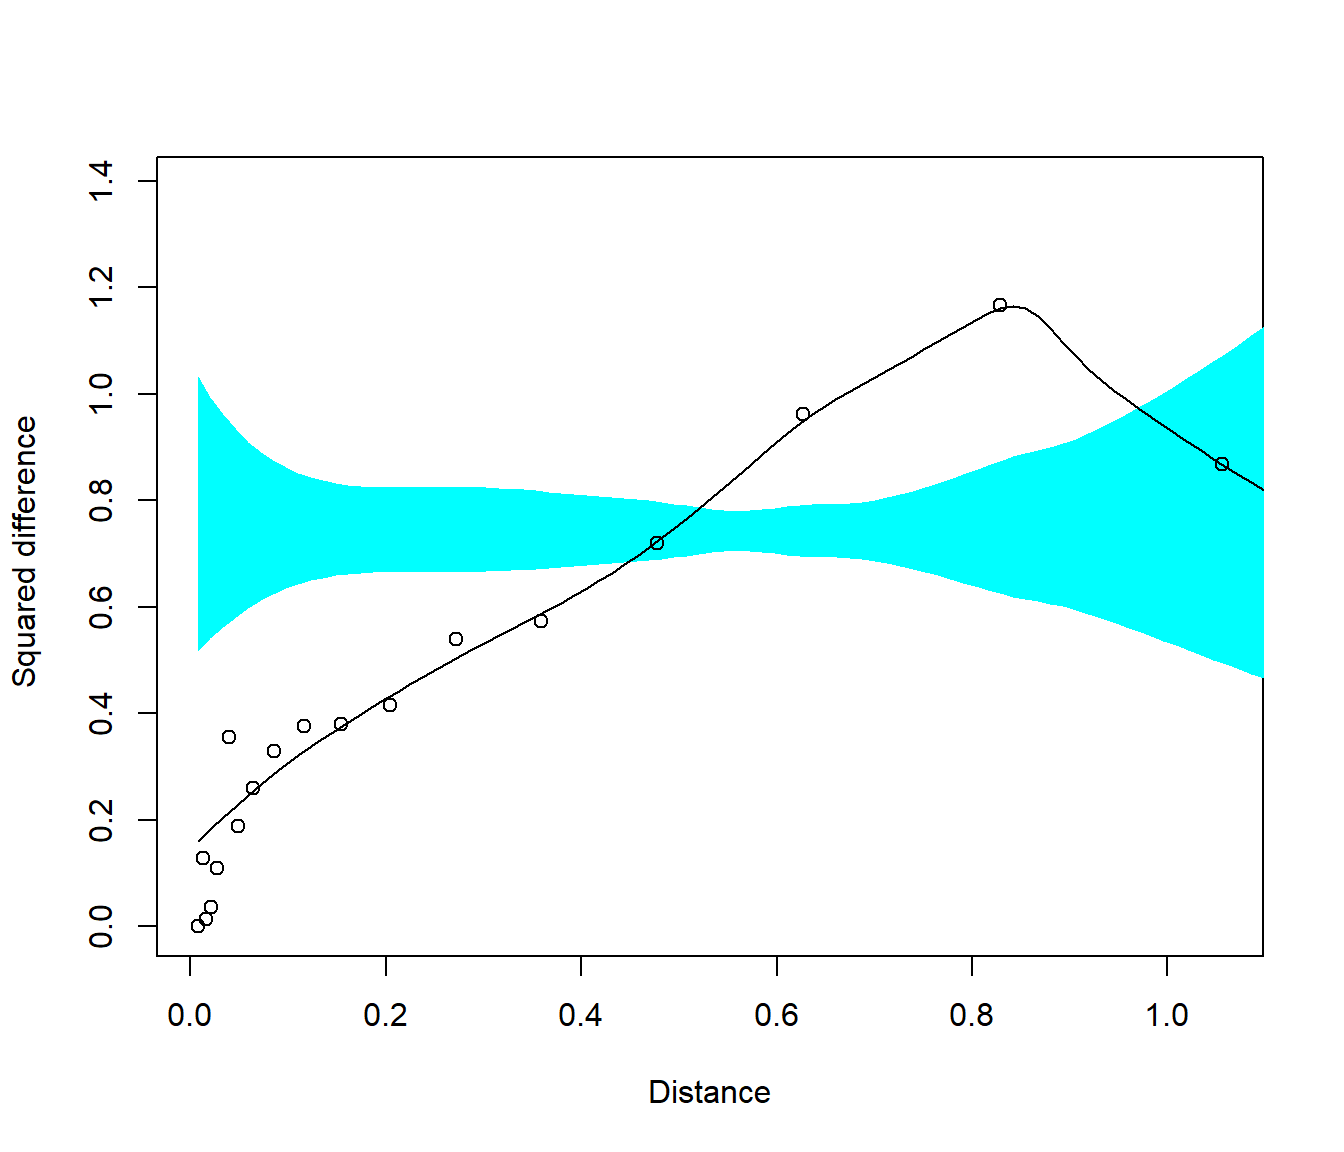
\includegraphics[width=0.7\linewidth]{11-sp_files/figure-latex/unnamed-chunk-18-1} \end{center}

\hypertarget{representaciones-gruxe1ficas}{%
\section{Representaciones gráficas}\label{representaciones-gruxe1ficas}}

\hypertarget{gruxe1ficos-estuxe1ndar}{%
\subsection{Gráficos estándar}\label{gruxe1ficos-estuxe1ndar}}

\begin{Shaded}
\begin{Highlighting}[]
\FunctionTok{plot}\NormalTok{(sdf, }\AttributeTok{axes =} \ConstantTok{TRUE}\NormalTok{, }\AttributeTok{pch =} \DecValTok{1}\NormalTok{)}
\FunctionTok{plot}\NormalTok{(galicia, }\AttributeTok{add =} \ConstantTok{TRUE}\NormalTok{)}
\end{Highlighting}
\end{Shaded}

\begin{center}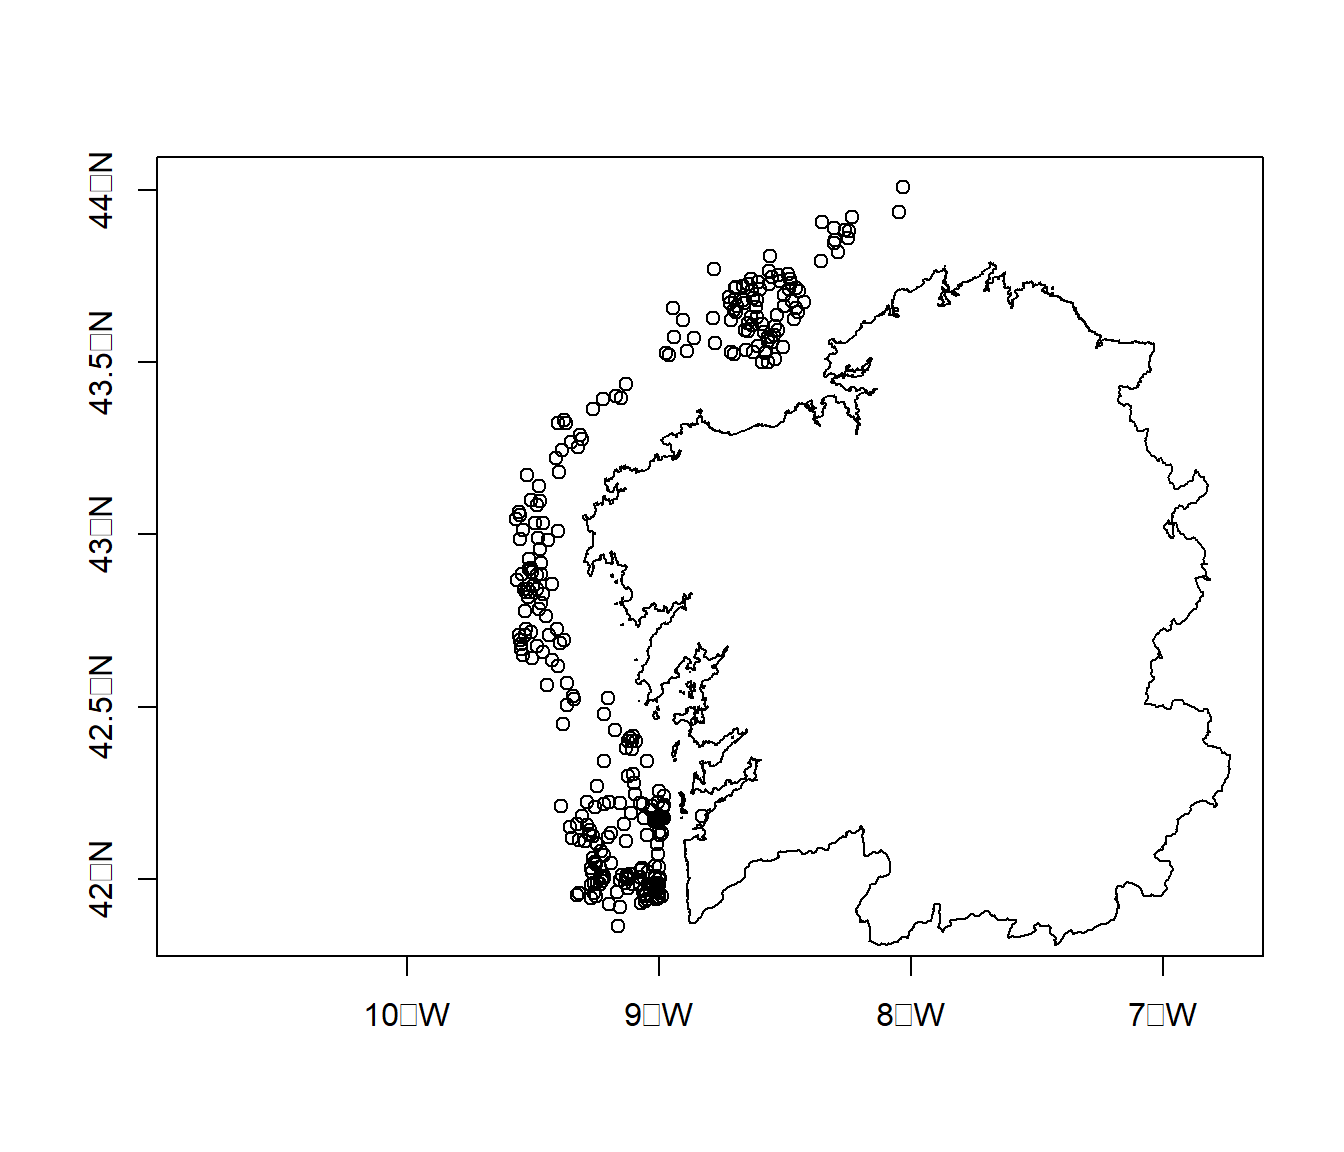
\includegraphics[width=0.7\linewidth]{11-sp_files/figure-latex/unnamed-chunk-19-1} \end{center}

Color en función de una variable categórica:

\begin{Shaded}
\begin{Highlighting}[]
\NormalTok{sdf}\SpecialCharTok{$}\NormalTok{ano }\OtherTok{\textless{}{-}} \FunctionTok{factor}\NormalTok{(sdf}\SpecialCharTok{$}\NormalTok{ano)   }\CommentTok{\# convertir año a factor}
\NormalTok{colores }\OtherTok{\textless{}{-}} \FunctionTok{c}\NormalTok{(}\StringTok{"blue"}\NormalTok{, }\StringTok{"yellow"}\NormalTok{, }\StringTok{"red"}\NormalTok{)}
\NormalTok{color }\OtherTok{\textless{}{-}}\NormalTok{ colores[}\FunctionTok{as.numeric}\NormalTok{(sdf}\SpecialCharTok{$}\NormalTok{ano)]}
\FunctionTok{plot}\NormalTok{(sdf, }\AttributeTok{axes =} \ConstantTok{TRUE}\NormalTok{, }\AttributeTok{col =}\NormalTok{ color, }\AttributeTok{pch =} \DecValTok{19}\NormalTok{)}
\FunctionTok{legend}\NormalTok{(}\StringTok{"topleft"}\NormalTok{, }\AttributeTok{fill =}\NormalTok{ colores, }\AttributeTok{legend =} \FunctionTok{levels}\NormalTok{(sdf}\SpecialCharTok{$}\NormalTok{ano), }\AttributeTok{bty =} \StringTok{"n"}\NormalTok{)}
\FunctionTok{plot}\NormalTok{(galicia, }\AttributeTok{add =} \ConstantTok{TRUE}\NormalTok{)}
\end{Highlighting}
\end{Shaded}

\begin{center}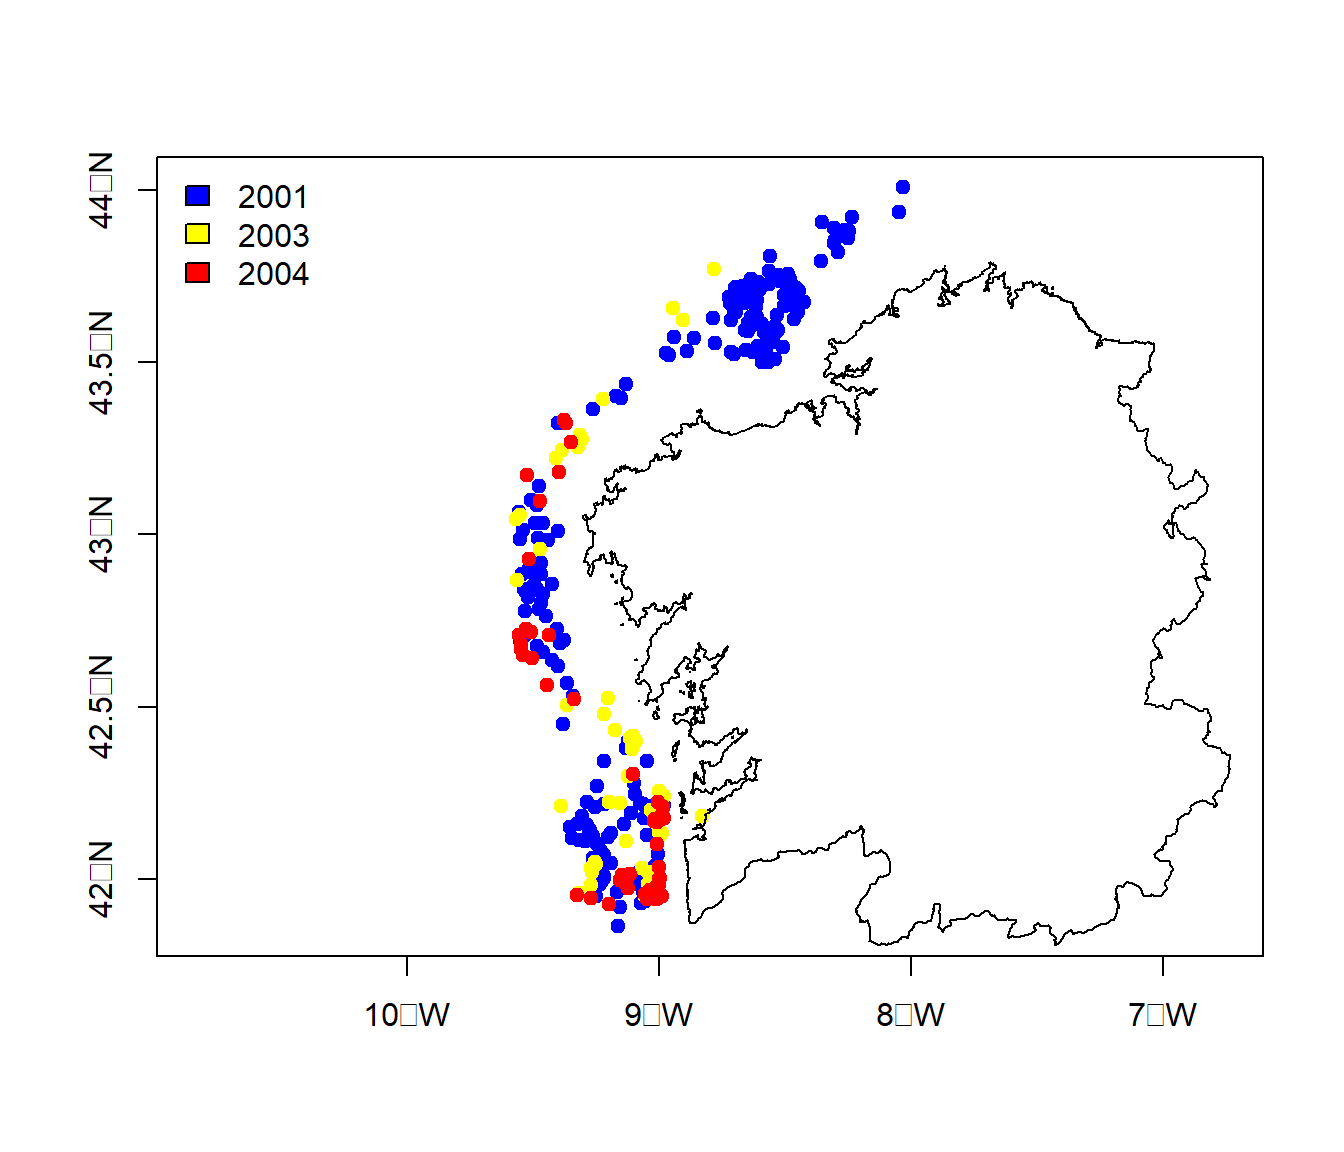
\includegraphics[width=0.7\linewidth]{11-sp_files/figure-latex/unnamed-chunk-20-1} \end{center}

Usando p.e. la función classIntervals del paquete classInt
se puede establecer los colores en función de una variable continua:

\begin{Shaded}
\begin{Highlighting}[]
\FunctionTok{library}\NormalTok{(classInt) }\CommentTok{\# install.packages(\textquotesingle{}classInt\textquotesingle{})}

\NormalTok{class.int }\OtherTok{\textless{}{-}} \FunctionTok{classIntervals}\NormalTok{(sdf}\SpecialCharTok{$}\NormalTok{lcpue, }\AttributeTok{n =} \DecValTok{5}\NormalTok{, }\AttributeTok{style =} \StringTok{"quantile"}\NormalTok{)}
\NormalTok{pal }\OtherTok{\textless{}{-}} \FunctionTok{c}\NormalTok{(}\StringTok{"blue"}\NormalTok{, }\StringTok{"red"}\NormalTok{)}
\CommentTok{\# plot(class.int, pal = pal)}

\NormalTok{class.col }\OtherTok{\textless{}{-}} \FunctionTok{findColours}\NormalTok{(class.int, }\AttributeTok{pal =}\NormalTok{ pal)}

\FunctionTok{plot}\NormalTok{(sdf, }\AttributeTok{col =}\NormalTok{ class.col, }\AttributeTok{pch =} \DecValTok{19}\NormalTok{)}
\FunctionTok{legend}\NormalTok{(}\StringTok{"topleft"}\NormalTok{, }\AttributeTok{fill =} \FunctionTok{attr}\NormalTok{(class.col, }\StringTok{"palette"}\NormalTok{), }
       \AttributeTok{legend =} \FunctionTok{names}\NormalTok{(}\FunctionTok{attr}\NormalTok{(class.col, }\StringTok{"table"}\NormalTok{)), }\AttributeTok{bty =} \StringTok{"n"}\NormalTok{)}
\FunctionTok{plot}\NormalTok{(galicia, }\AttributeTok{add =} \ConstantTok{TRUE}\NormalTok{)}
\end{Highlighting}
\end{Shaded}

\begin{center}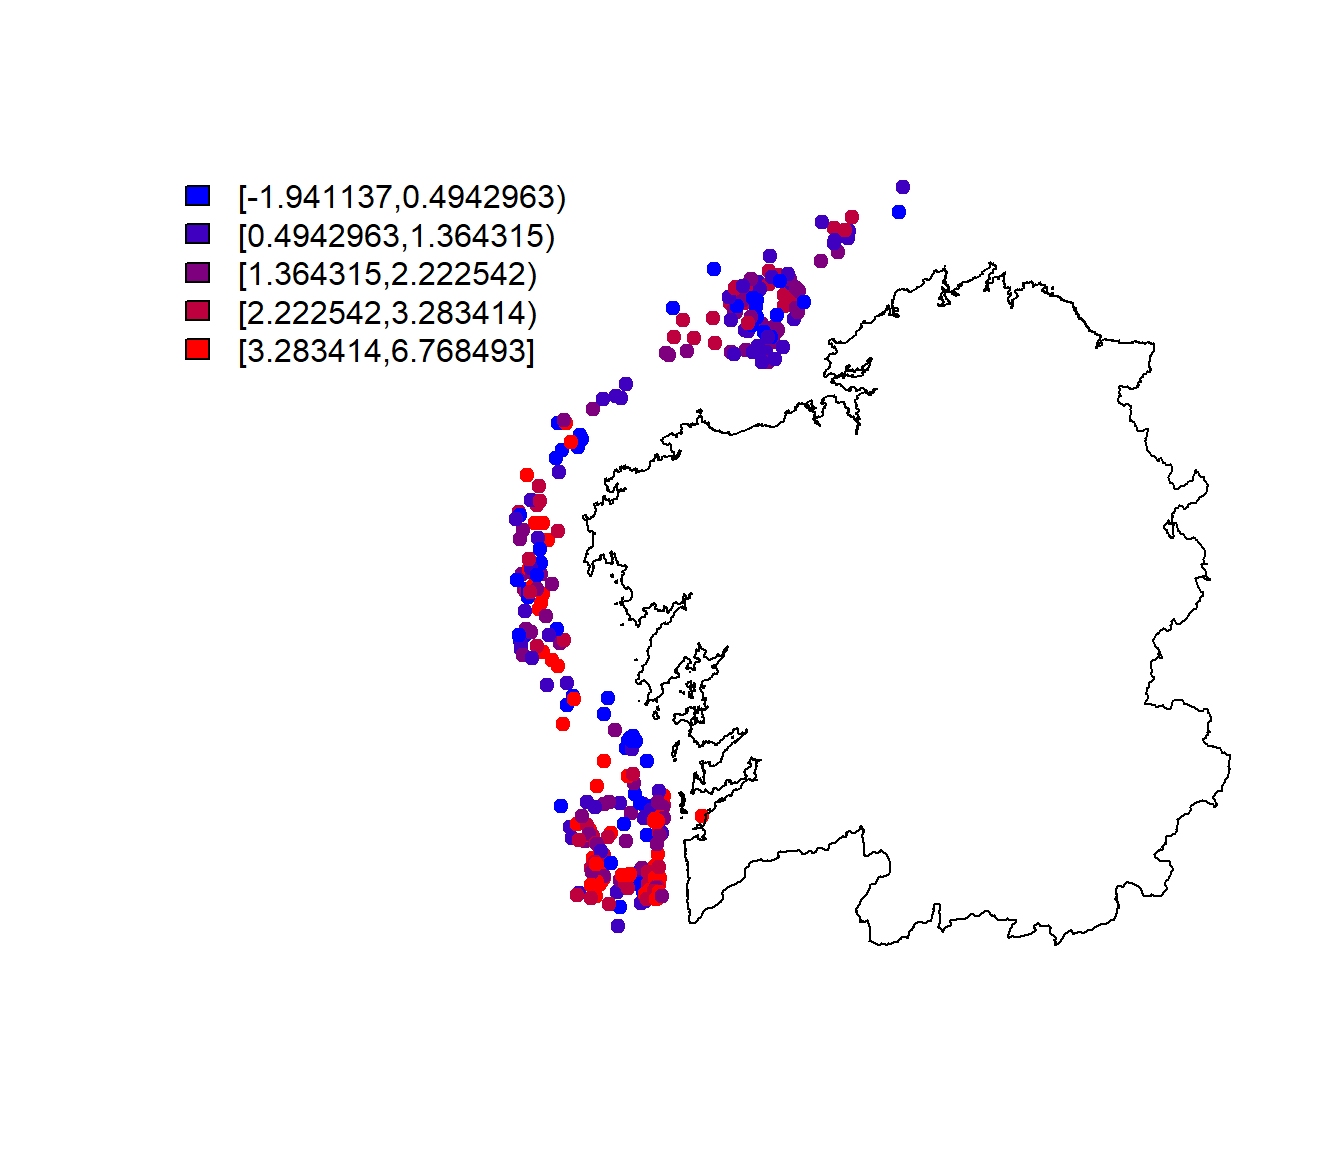
\includegraphics[width=0.7\linewidth]{11-sp_files/figure-latex/unnamed-chunk-21-1} \end{center}

\begin{Shaded}
\begin{Highlighting}[]
\CommentTok{\# methods(image) para rejillas}
\CommentTok{\# ver tambien splot, simage,... en library(npsp)}
\end{Highlighting}
\end{Shaded}

\hypertarget{gruxe1ficos-lattice-spplot}{%
\subsection{Gráficos lattice: spplot}\label{gruxe1ficos-lattice-spplot}}

\begin{itemize}
\item
  Ventajas: ``Ideales'' para las clases sp (para gráfico automáticos\ldots)
\item
  Inconveniente: los gráficos lattice requieren mayor tiempo de aprendizaje (dificultades para personalizarlos\ldots)
\end{itemize}

\begin{Shaded}
\begin{Highlighting}[]
\FunctionTok{library}\NormalTok{(lattice)}

\FunctionTok{spplot}\NormalTok{(sdf, }\StringTok{"lcpue"}\NormalTok{, }\AttributeTok{main =} \StringTok{"CPUE (escala logarítmica)"}\NormalTok{, }
       \AttributeTok{col.regions =} \FunctionTok{topo.colors}\NormalTok{(}\DecValTok{6}\NormalTok{), }\AttributeTok{cuts=}\DecValTok{5}\NormalTok{)}
\end{Highlighting}
\end{Shaded}

\begin{center}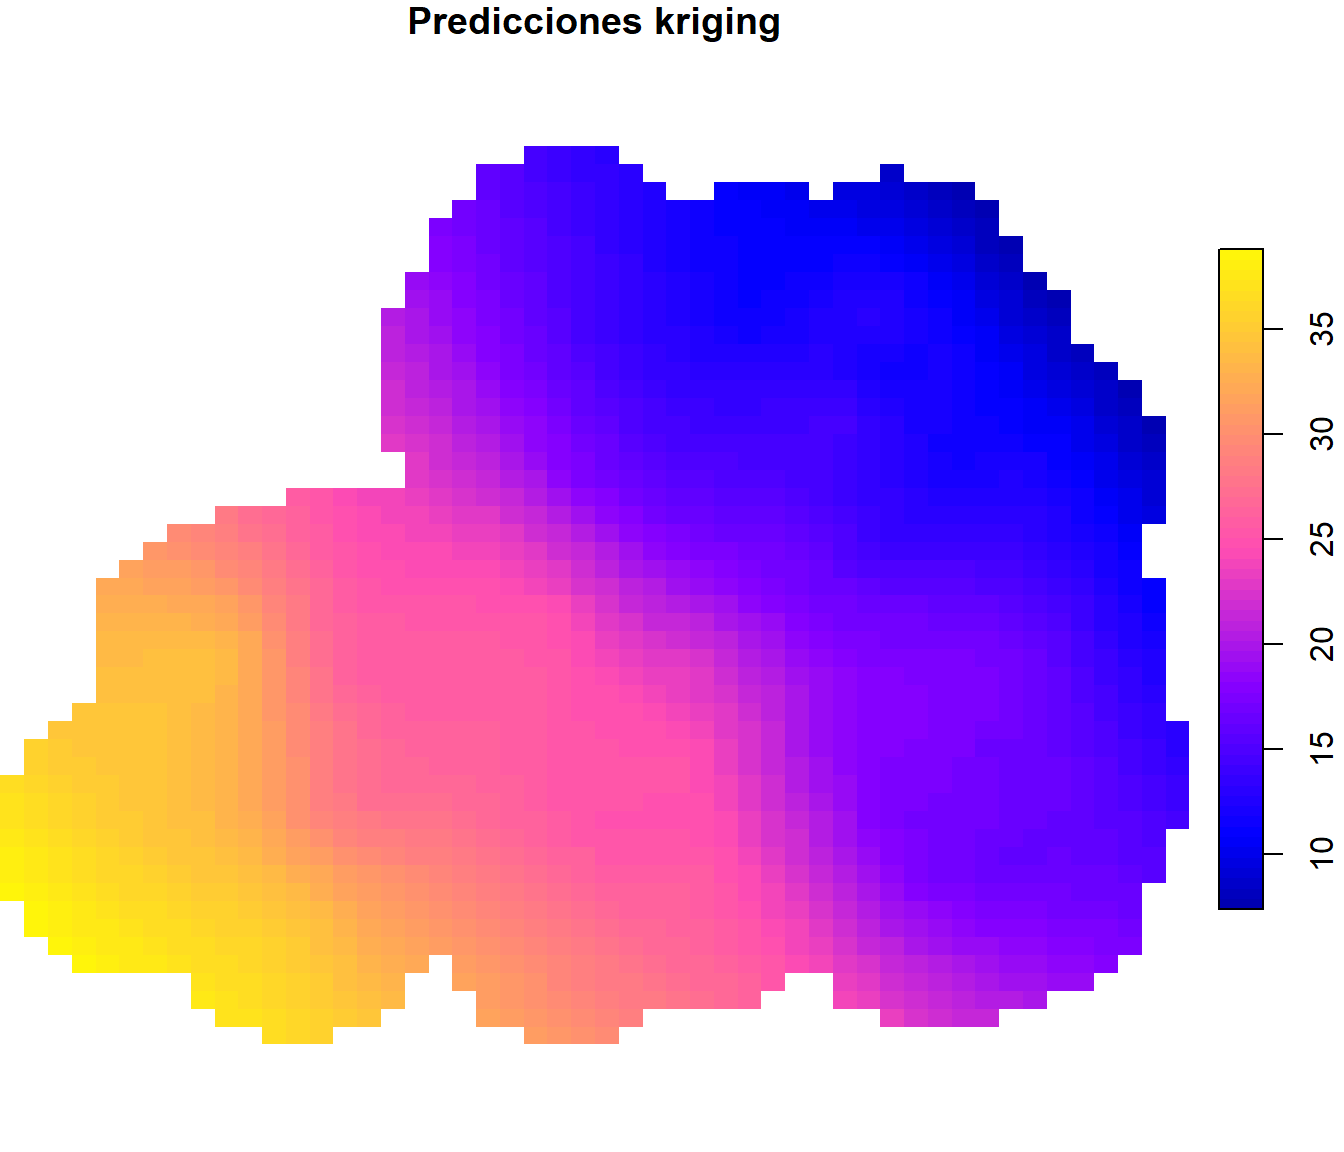
\includegraphics[width=0.7\linewidth]{11-sp_files/figure-latex/unnamed-chunk-22-1} \end{center}

\begin{Shaded}
\begin{Highlighting}[]
\FunctionTok{bubble}\NormalTok{(sdf, }\StringTok{"cpue"}\NormalTok{, }\AttributeTok{main =} \StringTok{"CPUE"}\NormalTok{) }
\end{Highlighting}
\end{Shaded}

\begin{center}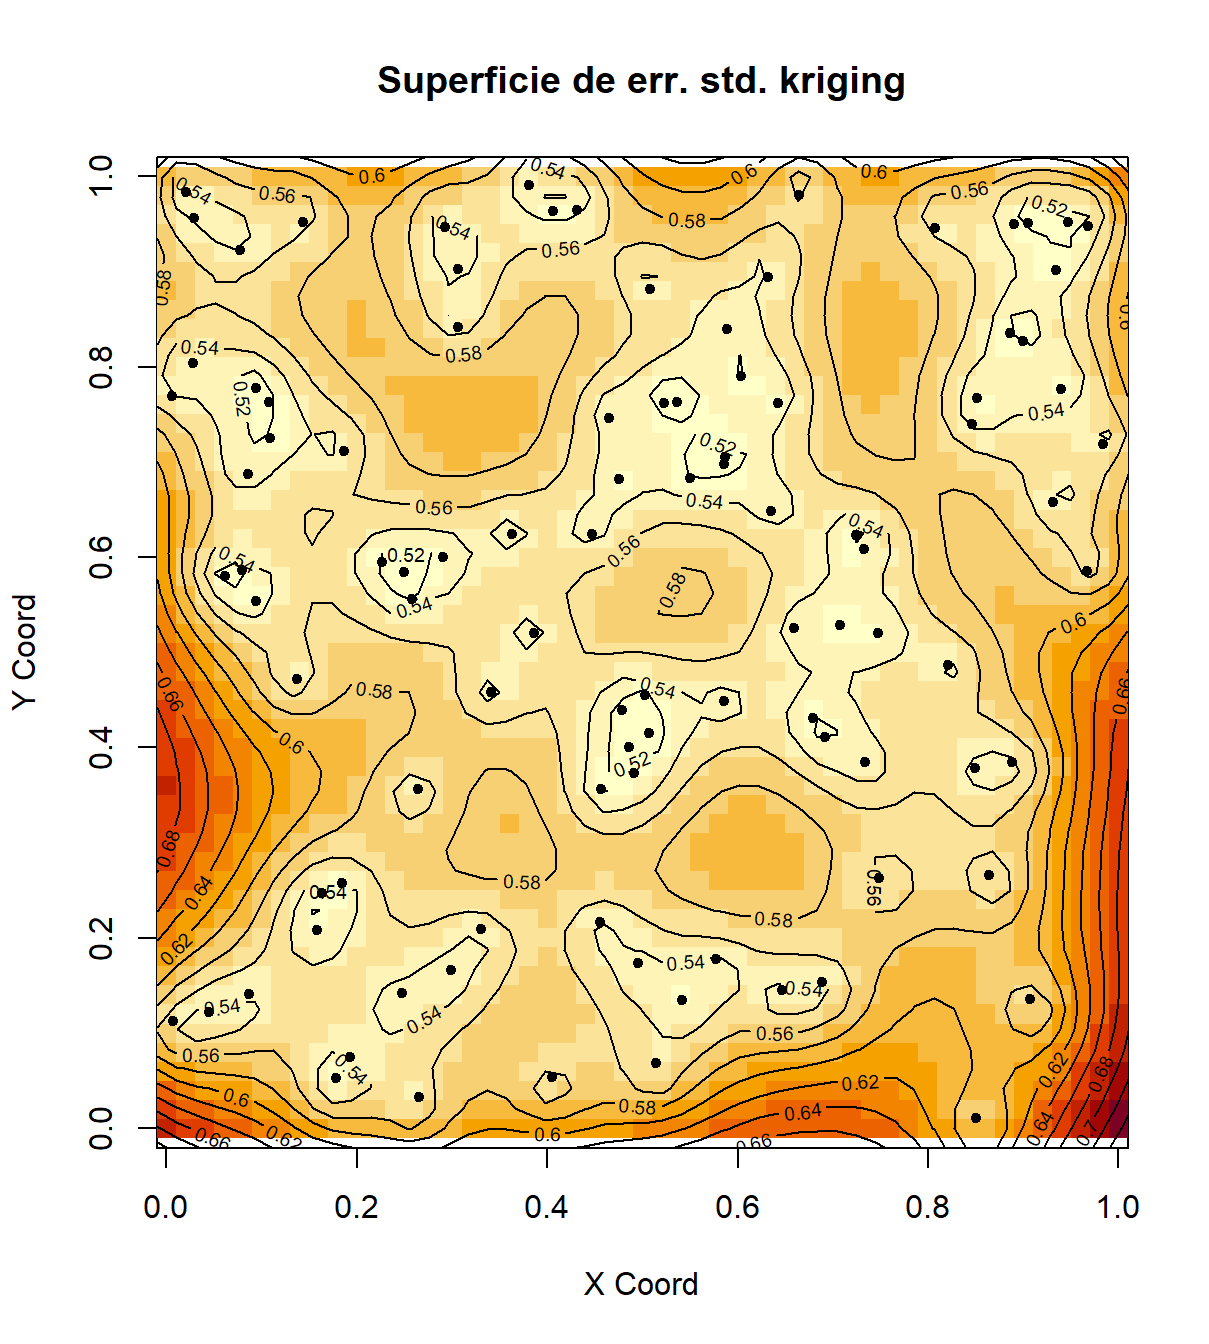
\includegraphics[width=0.7\linewidth]{11-sp_files/figure-latex/unnamed-chunk-22-2} \end{center}

Añadir perfil de Galicia:

\begin{Shaded}
\begin{Highlighting}[]
\NormalTok{sp.layout }\OtherTok{\textless{}{-}} \FunctionTok{list}\NormalTok{(}\StringTok{"sp.polygons"}\NormalTok{, galicia)   }\CommentTok{\# Para añadir elementos se utiliza el parámetro sp.layout}
\FunctionTok{spplot}\NormalTok{(sdf, }\StringTok{"lcpue"}\NormalTok{, }\AttributeTok{main =} \StringTok{"CPUE (escala logarítmica)"}\NormalTok{, }
       \AttributeTok{col.regions =} \FunctionTok{topo.colors}\NormalTok{(}\DecValTok{6}\NormalTok{), }\AttributeTok{cuts =} \DecValTok{5}\NormalTok{, }\AttributeTok{sp.layout =}\NormalTok{ sp.layout )}
\end{Highlighting}
\end{Shaded}

\begin{center}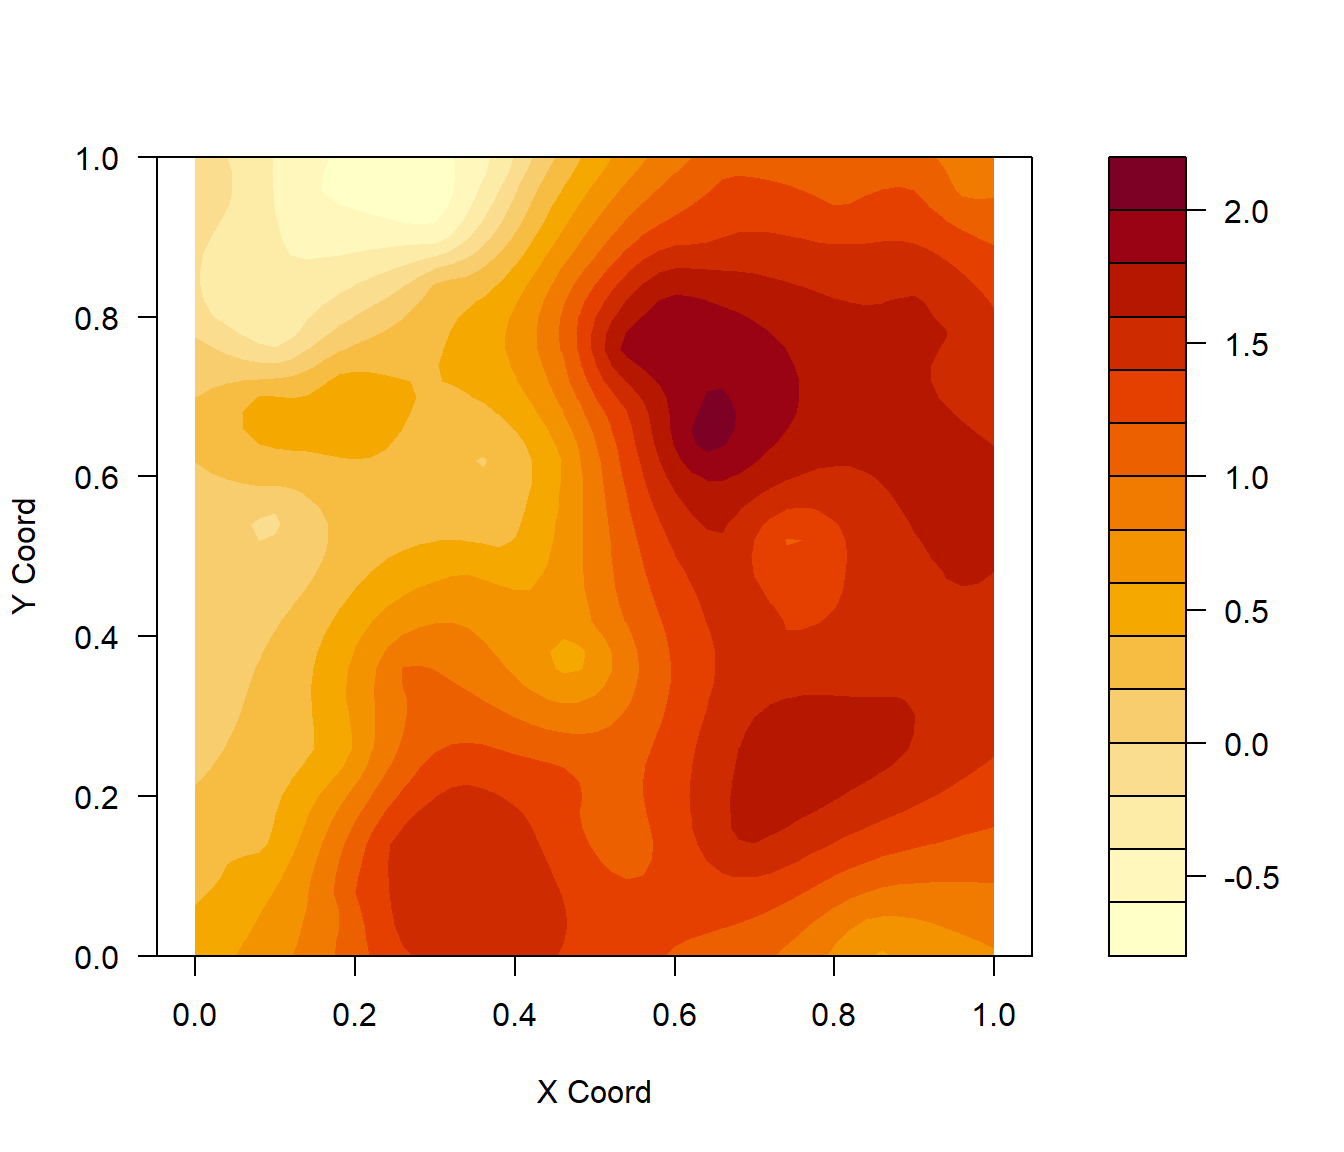
\includegraphics[width=0.7\linewidth]{11-sp_files/figure-latex/unnamed-chunk-23-1} \end{center}

Alternativamente gráficos ggplot (\href{https://ggplot2.tidyverse.org}{\texttt{ggplot2}}) con el paquete \href{https://paleolimbot.github.io/ggspatial}{\texttt{ggspatial}}\ldots{}

\hypertarget{intro-geoR}{%
\chapter{\texorpdfstring{Introducción al paquete \textbf{geoR}}{Introducción al paquete geoR}}\label{intro-geoR}}

El paquete \href{http://www.leg.ufpr.br/geoR}{\texttt{geoR}} proporciona herramientas para el análisis de datos
geoestadísticos en \texttt{R}
(otra alternativa es el paquete \href{http://r-spatial.github.io/gstat}{\texttt{gstat}}, por ejemplo\ldots).
A continuación se ilustran algunas de las capacidades de este paquete.

\hypertarget{inicio-de-una-sesiuxf3n-y-de-carga-de-datos}{%
\section{Inicio de una sesión y de carga de datos}\label{inicio-de-una-sesiuxf3n-y-de-carga-de-datos}}

Después de iniciar la sesión R, cargar \texttt{geoR} con el comando \texttt{library} (o
\texttt{require}). Si el paquete se carga correctamente aparece un mensaje.

\begin{Shaded}
\begin{Highlighting}[]
\FunctionTok{library}\NormalTok{(geoR)}
\end{Highlighting}
\end{Shaded}

\begin{verbatim}
## --------------------------------------------------------------
##  Analysis of Geostatistical Data
##  For an Introduction to geoR go to http://www.leg.ufpr.br/geoR
##  geoR version 1.8-1 (built on 2020-02-08) is now loaded
## --------------------------------------------------------------
\end{verbatim}

\hypertarget{archivos-de-datos}{%
\subsection{Archivos de datos}\label{archivos-de-datos}}

Normalmente, los datos se almacenan como un objeto (una lista) de la
clase \texttt{geodata}. Un objeto de esta clase contiene obligatoriamente dos
elementos:

\begin{itemize}
\item
  \texttt{\$coords}: las coordenadas de las posiciones de los datos.
\item
  \texttt{\$data}: los valores observados de la variables.
\end{itemize}

Opcionalmente pueden tener otros elementos, como covariables
y coordenadas de las fronteras de la zona de estudio.

Hay algunos conjuntos de datos incluidos en el paquete de distribución.

\begin{Shaded}
\begin{Highlighting}[]
\CommentTok{\# data()                    \# lista todos los conjuntos de datos disponibles}
\CommentTok{\# data(package = "geoR")    \# lista los conjuntos de datos en el paquete geoR}

\FunctionTok{data}\NormalTok{(wolfcamp)              }\CommentTok{\# carga el archivo de datos wolfcamp}
\FunctionTok{summary}\NormalTok{(wolfcamp)}
\end{Highlighting}
\end{Shaded}

\begin{verbatim}
## Number of data points: 85 
## 
## Coordinates summary
##       Coord.X   Coord.Y
## min -233.7217 -145.7884
## max  181.5314  136.4061
## 
## Distance summary
##         min         max 
##   0.3669819 436.2067085 
## 
## Data summary
##      Min.   1st Qu.    Median      Mean   3rd Qu.      Max. 
##  312.1095  471.8218  547.7156  610.2845  774.1778 1088.4209
\end{verbatim}

Se pueden importar directamente un archivo de datos en formato texto:

\begin{Shaded}
\begin{Highlighting}[]
\NormalTok{ncep }\OtherTok{\textless{}{-}} \FunctionTok{read.geodata}\NormalTok{(}\StringTok{\textquotesingle{}ncep.txt\textquotesingle{}}\NormalTok{, }\AttributeTok{header =} \ConstantTok{FALSE}\NormalTok{, }\AttributeTok{coords.col =} \DecValTok{1}\SpecialCharTok{:}\DecValTok{2}\NormalTok{, }\AttributeTok{data.col =} \DecValTok{4}\NormalTok{)}
\CommentTok{\# plot(ncep)}
\CommentTok{\# summary(ncep)}
\end{Highlighting}
\end{Shaded}

También se puede convertir un \texttt{data.frame} a un objeto \texttt{geodata}:

\begin{Shaded}
\begin{Highlighting}[]
\NormalTok{ncep.df }\OtherTok{\textless{}{-}} \FunctionTok{read.table}\NormalTok{(}\StringTok{\textquotesingle{}ncep.txt\textquotesingle{}}\NormalTok{, }\AttributeTok{header =} \ConstantTok{FALSE}\NormalTok{)}
\FunctionTok{names}\NormalTok{(ncep.df) }\OtherTok{\textless{}{-}} \FunctionTok{c}\NormalTok{(}\StringTok{\textquotesingle{}x\textquotesingle{}}\NormalTok{, }\StringTok{\textquotesingle{}y\textquotesingle{}}\NormalTok{, }\StringTok{\textquotesingle{}t\textquotesingle{}}\NormalTok{, }\StringTok{\textquotesingle{}z\textquotesingle{}}\NormalTok{)}
\CommentTok{\# str(ncep.df)}
\CommentTok{\# Nota: los datos son espacio{-}temporales, pero geoR sólo admite datos 2D}

\NormalTok{datgeo }\OtherTok{\textless{}{-}} \FunctionTok{as.geodata}\NormalTok{(ncep.df, }\AttributeTok{coords.col =} \DecValTok{1}\SpecialCharTok{:}\DecValTok{2}\NormalTok{, }\AttributeTok{data.col =} \DecValTok{4}\NormalTok{)}
\CommentTok{\# plot(datgeo)}
\CommentTok{\# summary(datgeo)}
\end{Highlighting}
\end{Shaded}

O objetos de datos espaciales (entre ellos los compatibles del paquete \texttt{sp}),
por ejemplo el siguiente código crea un objeto \texttt{SpatialPointsDataFrame}
y lo convierte a \texttt{geodata}:

\begin{Shaded}
\begin{Highlighting}[]
\FunctionTok{library}\NormalTok{(sp)}
\FunctionTok{load}\NormalTok{(}\StringTok{"caballa.galicia.RData"}\NormalTok{)}
\FunctionTok{coordinates}\NormalTok{(caballa.galicia) }\OtherTok{\textless{}{-}} \FunctionTok{c}\NormalTok{(}\StringTok{"x"}\NormalTok{,}\StringTok{"y"}\NormalTok{)}
\FunctionTok{proj4string}\NormalTok{(caballa.galicia) }\OtherTok{\textless{}{-}} \FunctionTok{CRS}\NormalTok{(}\StringTok{"+proj=longlat +ellps=WGS84"}\NormalTok{)}

\NormalTok{datgeo }\OtherTok{\textless{}{-}} \FunctionTok{as.geodata}\NormalTok{(caballa.galicia[}\StringTok{"lcpue"}\NormalTok{])}
\CommentTok{\# Problemas con coordenadas duplicadas  (ver ?duplicated)}
\CommentTok{\# plot(datgeo)}
\CommentTok{\# summary(datgeo)     }
\end{Highlighting}
\end{Shaded}

En la documentación de las funciones \texttt{as.geodata} y \texttt{read.geodata}
hay más información sobre cómo importar/convertir datos.

\hypertarget{anuxe1lisis-descriptivo-de-datos-geoestaduxedsticos}{%
\section{Análisis descriptivo de datos geoestadísticos}\label{anuxe1lisis-descriptivo-de-datos-geoestaduxedsticos}}

Como se mostró anteriormente, el método \texttt{summary} proporciona un breve resumen
descriptivo de los datos (ver \texttt{?summary.geodata}).

La función \texttt{plot()} genera por defecto gráficos de los
valores en las posiciones espaciales (distinguiendo según cuartiles),
los datos frente a las coordenadas y un histograma de los datos:

\begin{Shaded}
\begin{Highlighting}[]
\FunctionTok{plot}\NormalTok{(wolfcamp)}
\end{Highlighting}
\end{Shaded}

\begin{center}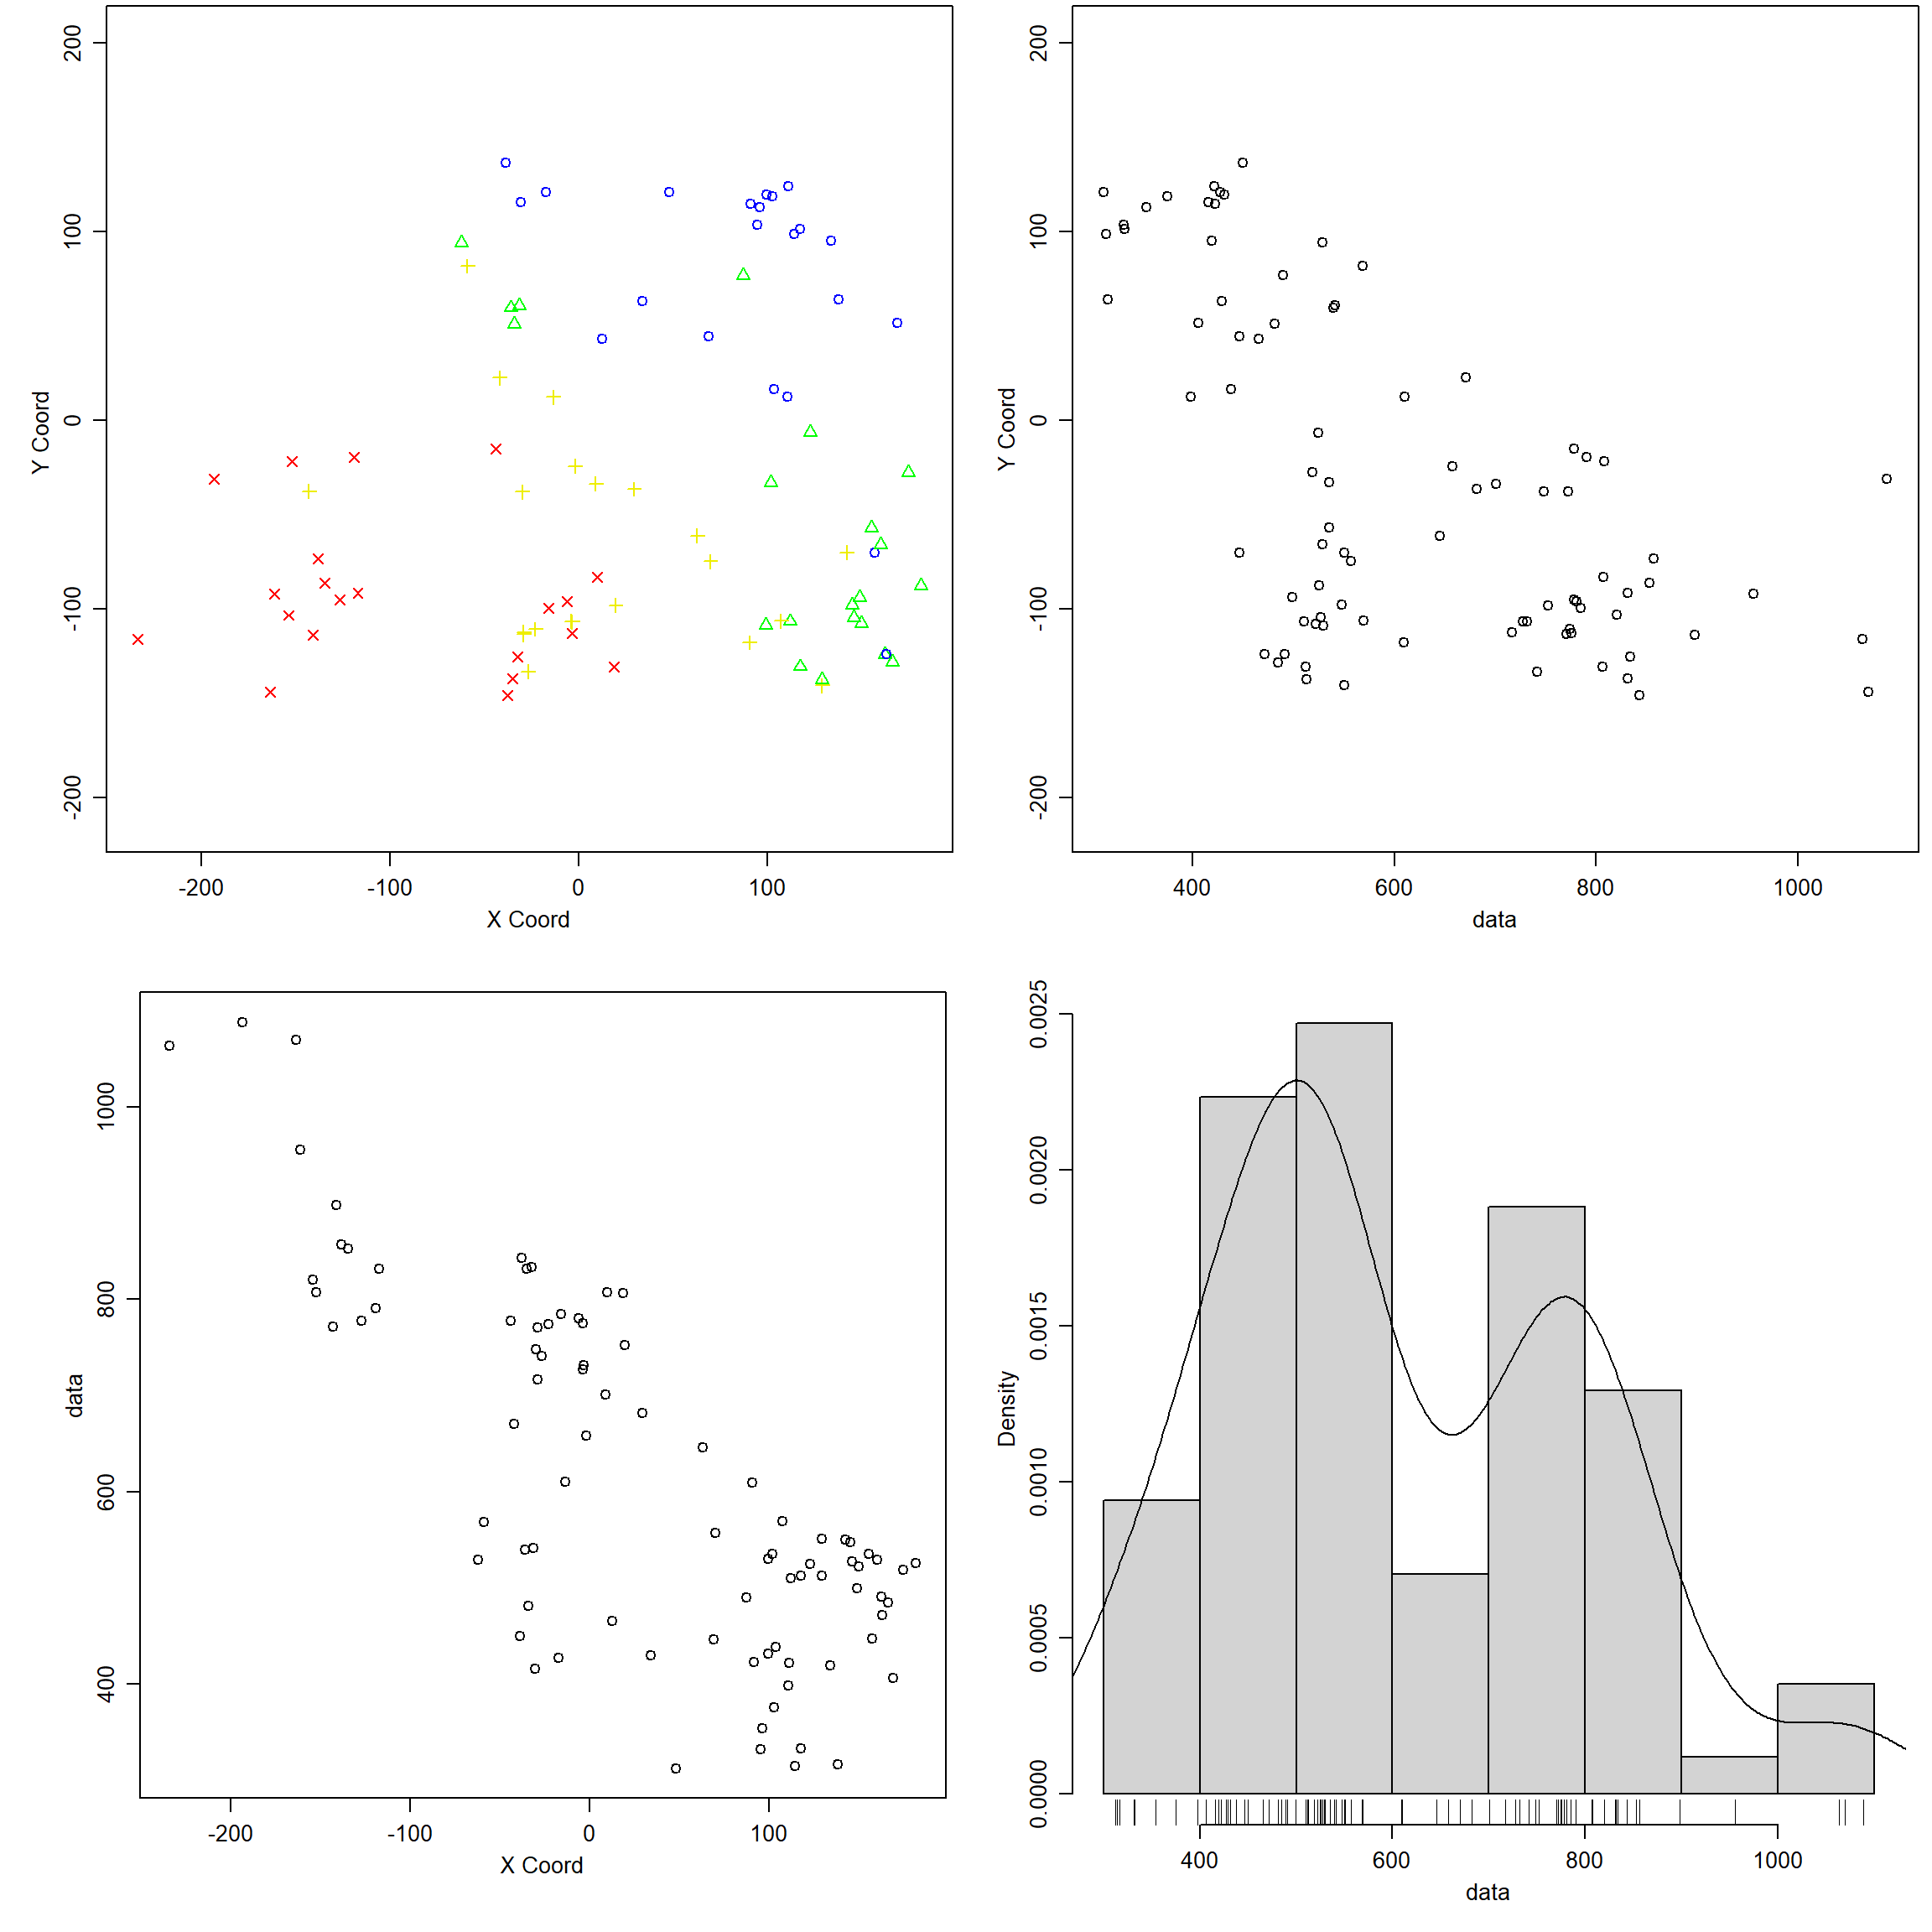
\includegraphics[width=0.9\linewidth]{12-geor_files/figure-latex/plot-geo1-1} \end{center}

Los gráficos de dispersión de los datos frente a las coordenadas nos pueden ayudar
a determinar si hay una tendencia. También, en lugar del histograma,
nos puede interesar un gráfico de dispersión 3D

\begin{Shaded}
\begin{Highlighting}[]
\FunctionTok{plot}\NormalTok{(wolfcamp, }\AttributeTok{lowess =} \ConstantTok{TRUE}\NormalTok{, }\AttributeTok{scatter3d =} \ConstantTok{TRUE}\NormalTok{) }
\end{Highlighting}
\end{Shaded}

\begin{center}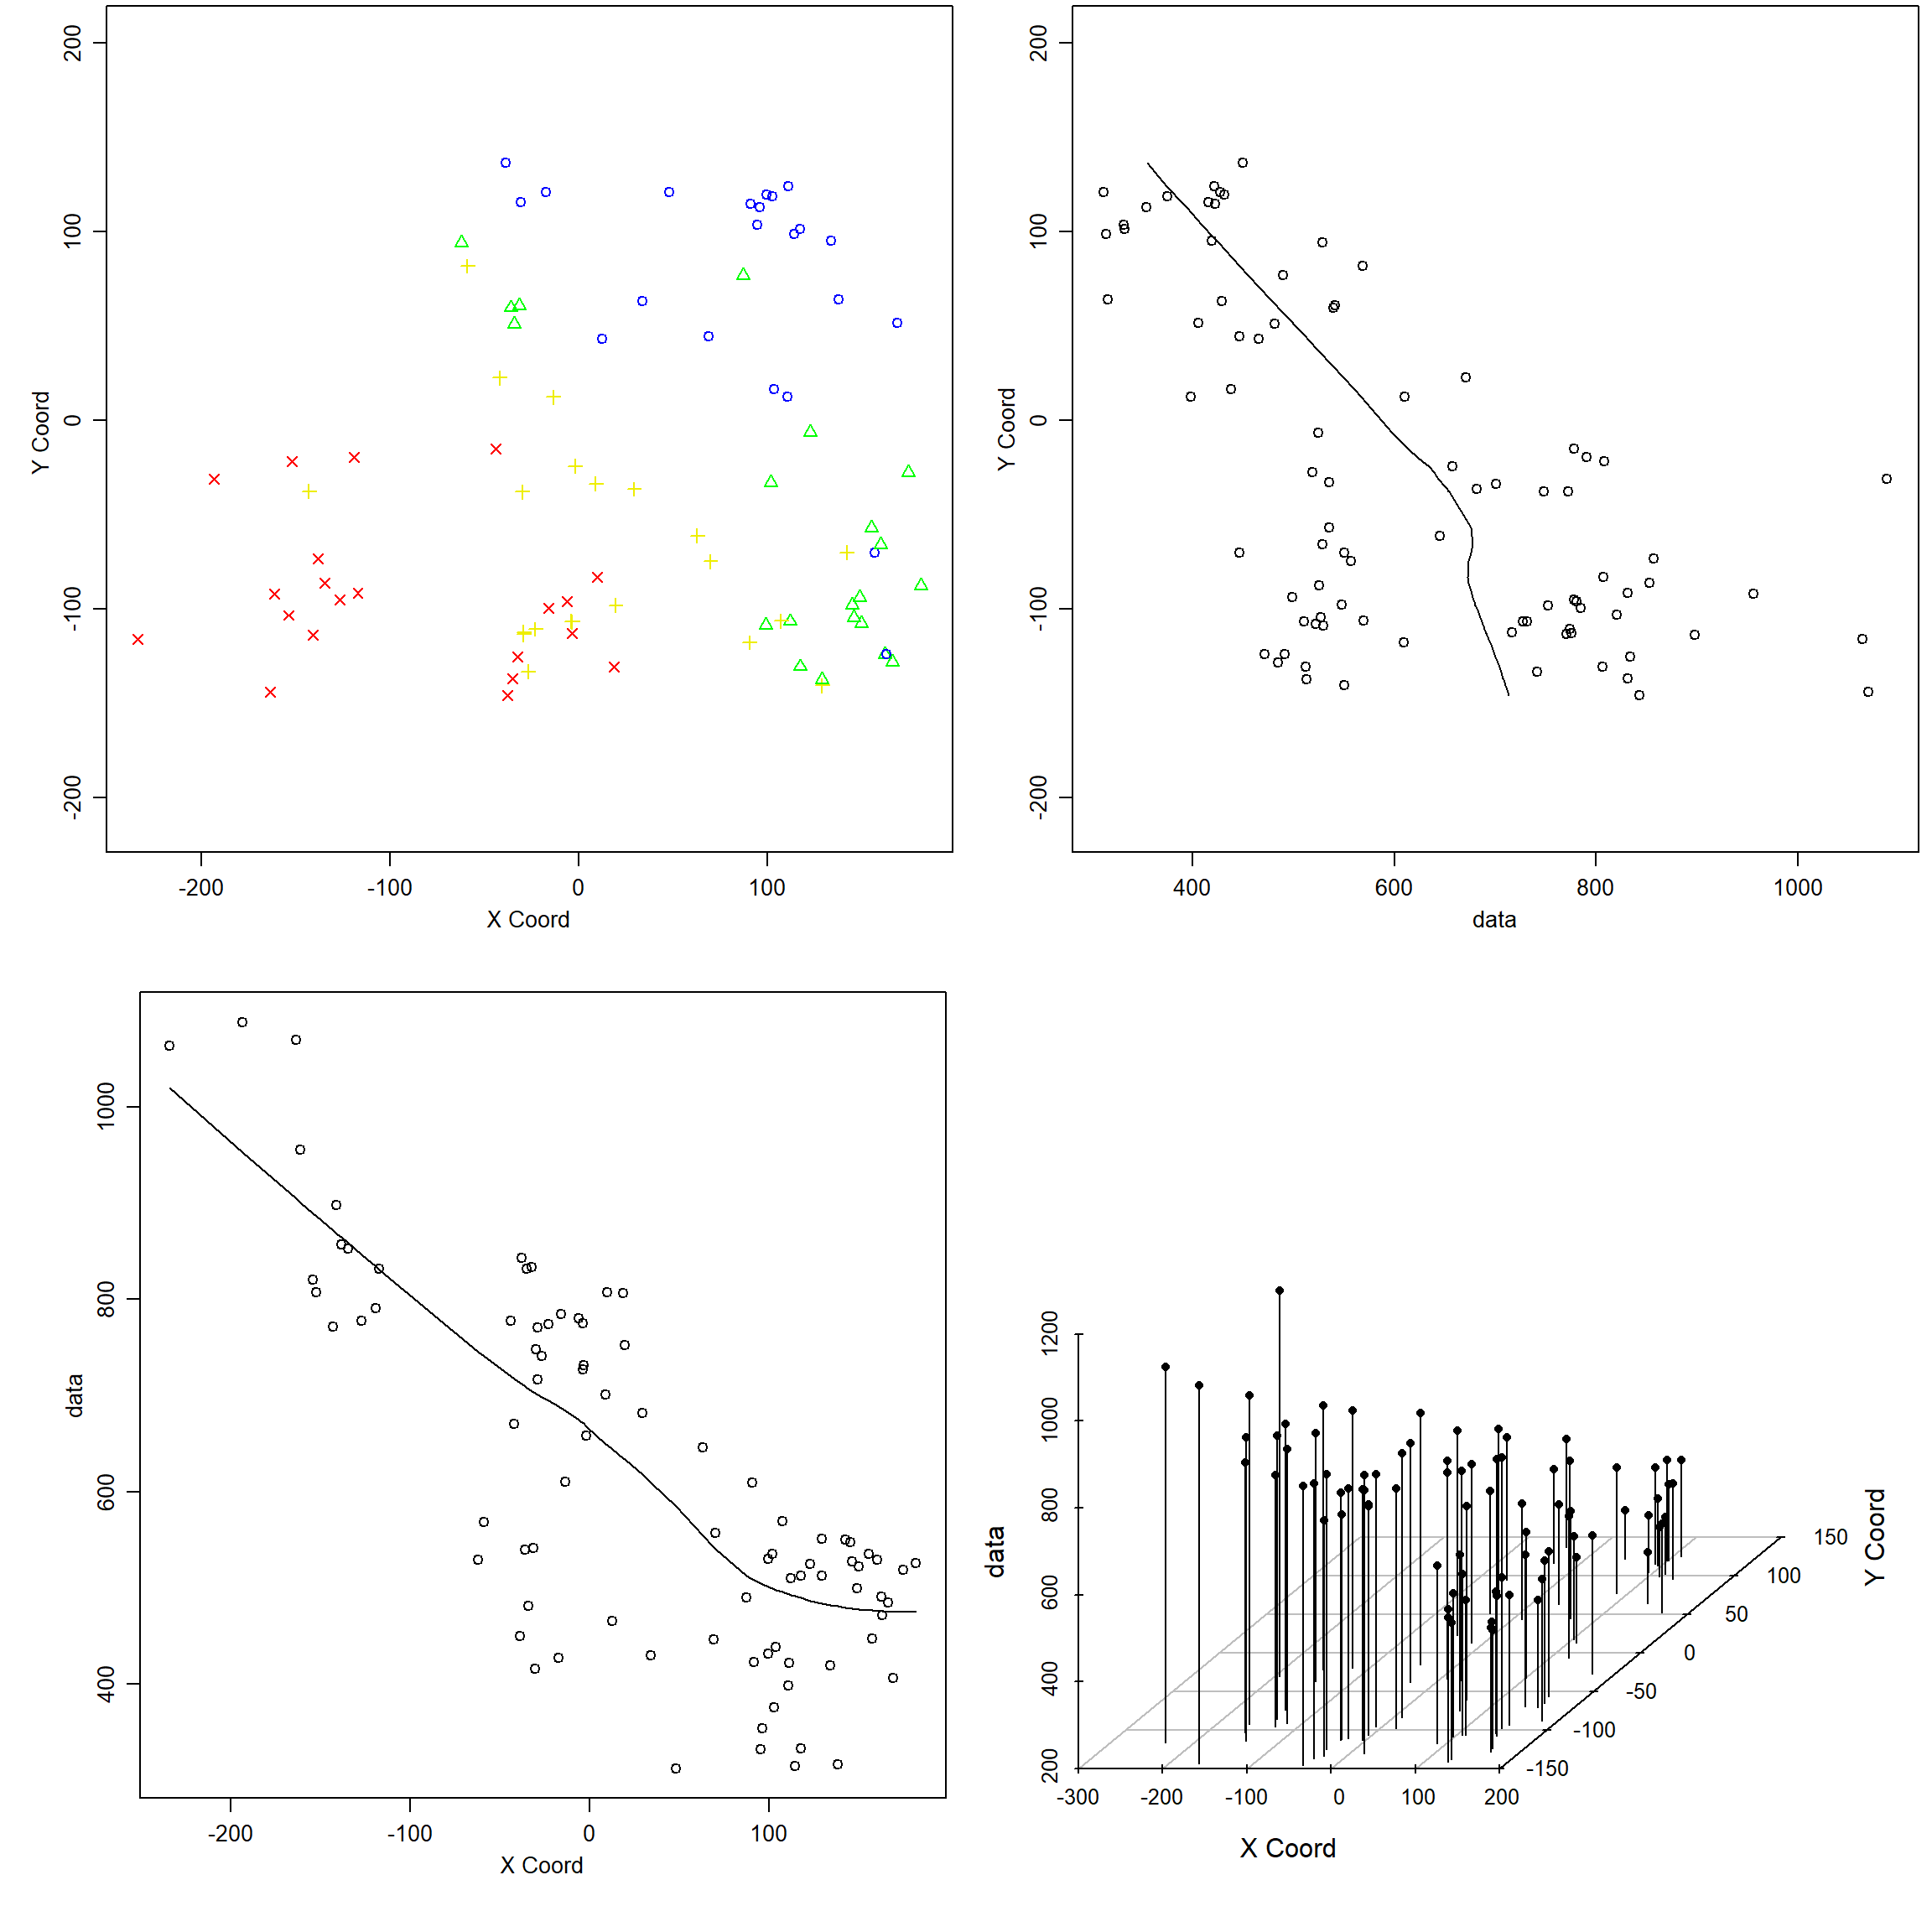
\includegraphics[width=0.9\linewidth]{12-geor_files/figure-latex/plot-geo2-1} \end{center}

Si se asume que hay una tendencia puede interesar eliminarla:

\begin{Shaded}
\begin{Highlighting}[]
\FunctionTok{plot}\NormalTok{(wolfcamp, }\AttributeTok{trend=}\SpecialCharTok{\textasciitilde{}}\NormalTok{coords)}
\end{Highlighting}
\end{Shaded}

\begin{center}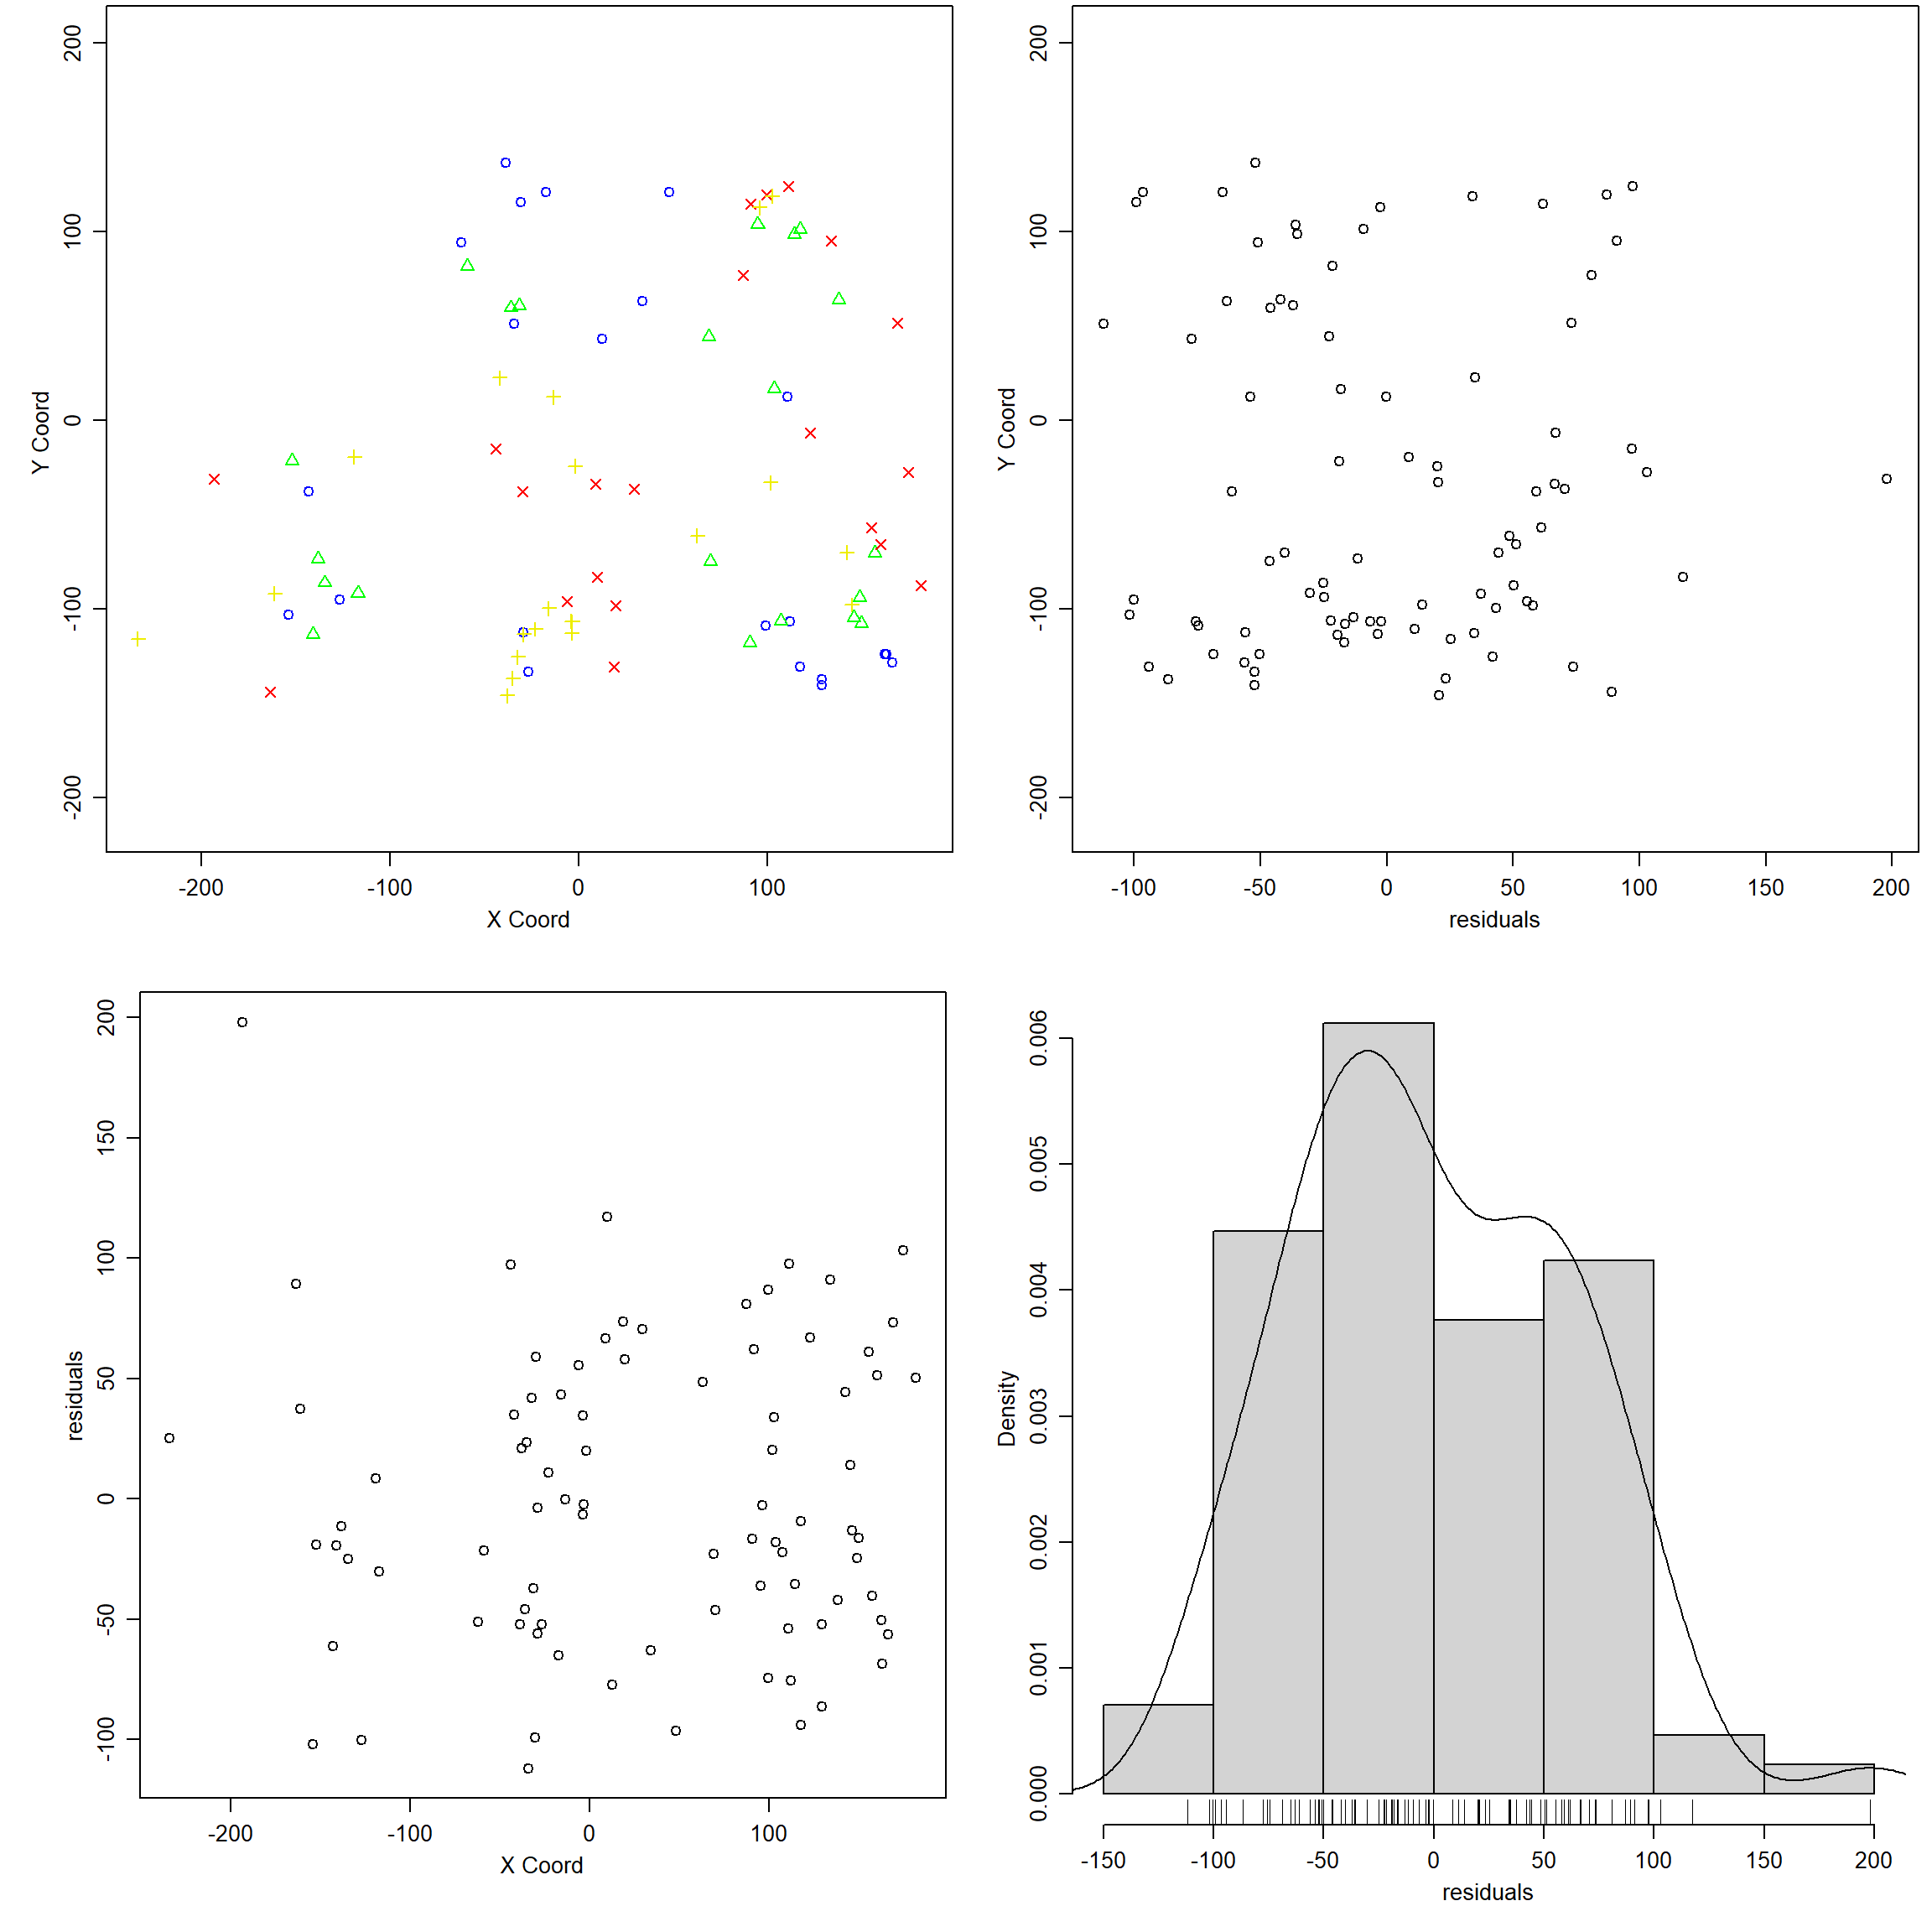
\includegraphics[width=0.9\linewidth]{12-geor_files/figure-latex/plot-geo3-1} \end{center}

El comando \texttt{points(geodata)} (función \texttt{points.geodata}) genera un gráfico con
las posiciones de los datos (y por defecto con el tamaño de los puntos proporcional
al valor):

\begin{Shaded}
\begin{Highlighting}[]
\FunctionTok{points}\NormalTok{(wolfcamp)}
\end{Highlighting}
\end{Shaded}

\begin{center}\includegraphics[width=0.7\linewidth]{12-geor_files/figure-latex/unnamed-chunk-7-1} \end{center}

Se pueden establecer los tamaños de los puntos, simbolos y colores a
partir de los valores de los datos. Por ejemplo, para los puntos, empleando el argumento:
\texttt{pt.divide\ =\ c("data.proportional",\ "rank.proportional",\ "quintiles",}
\texttt{"quartiles",\ "deciles",\ "equal")}.

\begin{Shaded}
\begin{Highlighting}[]
\FunctionTok{points}\NormalTok{(wolfcamp, }\AttributeTok{col =} \StringTok{"gray"}\NormalTok{, }\AttributeTok{pt.divide =} \StringTok{"equal"}\NormalTok{)}
\end{Highlighting}
\end{Shaded}

\begin{center}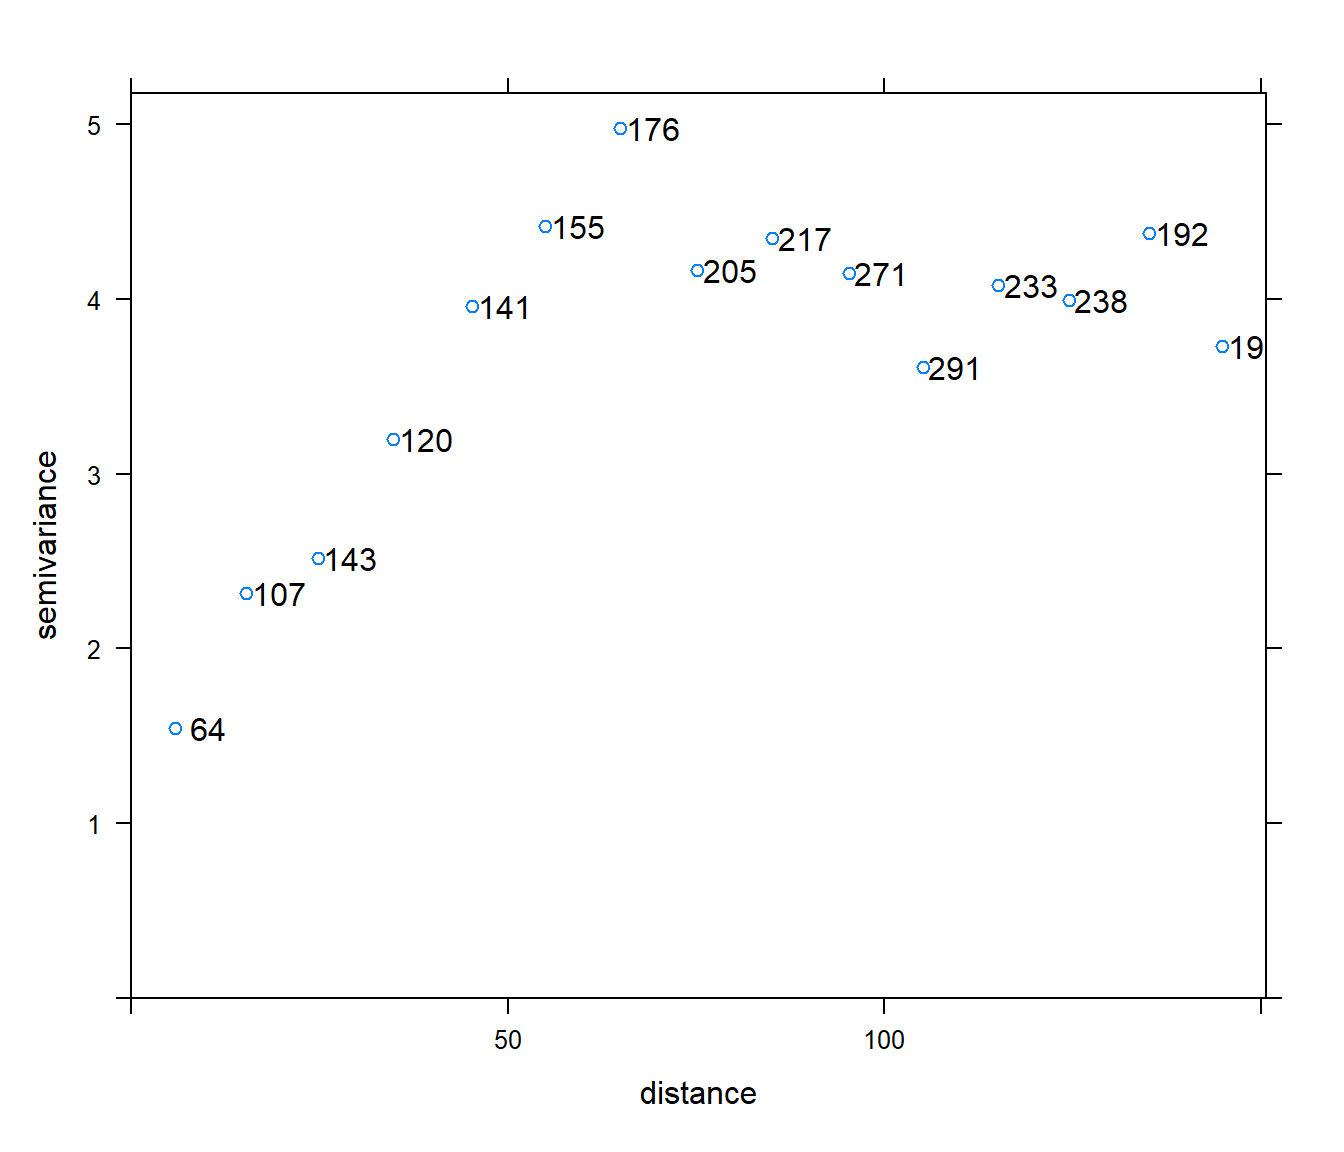
\includegraphics[width=0.7\linewidth]{12-geor_files/figure-latex/unnamed-chunk-8-1} \end{center}

\hypertarget{modelado-de-la-dependencia}{%
\section{Modelado de la dependencia}\label{modelado-de-la-dependencia}}

En la primera parte de esta sección consideraremos un proceso espacial sin
tendencia:

\begin{Shaded}
\begin{Highlighting}[]
\FunctionTok{data}\NormalTok{(s100) }\CommentTok{\# Cargar datos estacionarios}
\FunctionTok{summary}\NormalTok{(s100)}
\end{Highlighting}
\end{Shaded}

\begin{verbatim}
## Number of data points: 100 
## 
## Coordinates summary
##         Coord.X    Coord.Y
## min 0.005638006 0.01091027
## max 0.983920544 0.99124979
## 
## Distance summary
##         min         max 
## 0.007640962 1.278175109 
## 
## Data summary
##       Min.    1st Qu.     Median       Mean    3rd Qu.       Max. 
## -1.1676955  0.2729882  1.1045936  0.9307179  1.6101707  2.8678969 
## 
## Other elements in the geodata object
## [1] "cov.model" "nugget"    "cov.pars"  "kappa"     "lambda"
\end{verbatim}

\begin{Shaded}
\begin{Highlighting}[]
\FunctionTok{plot}\NormalTok{(s100)}
\end{Highlighting}
\end{Shaded}

\begin{center}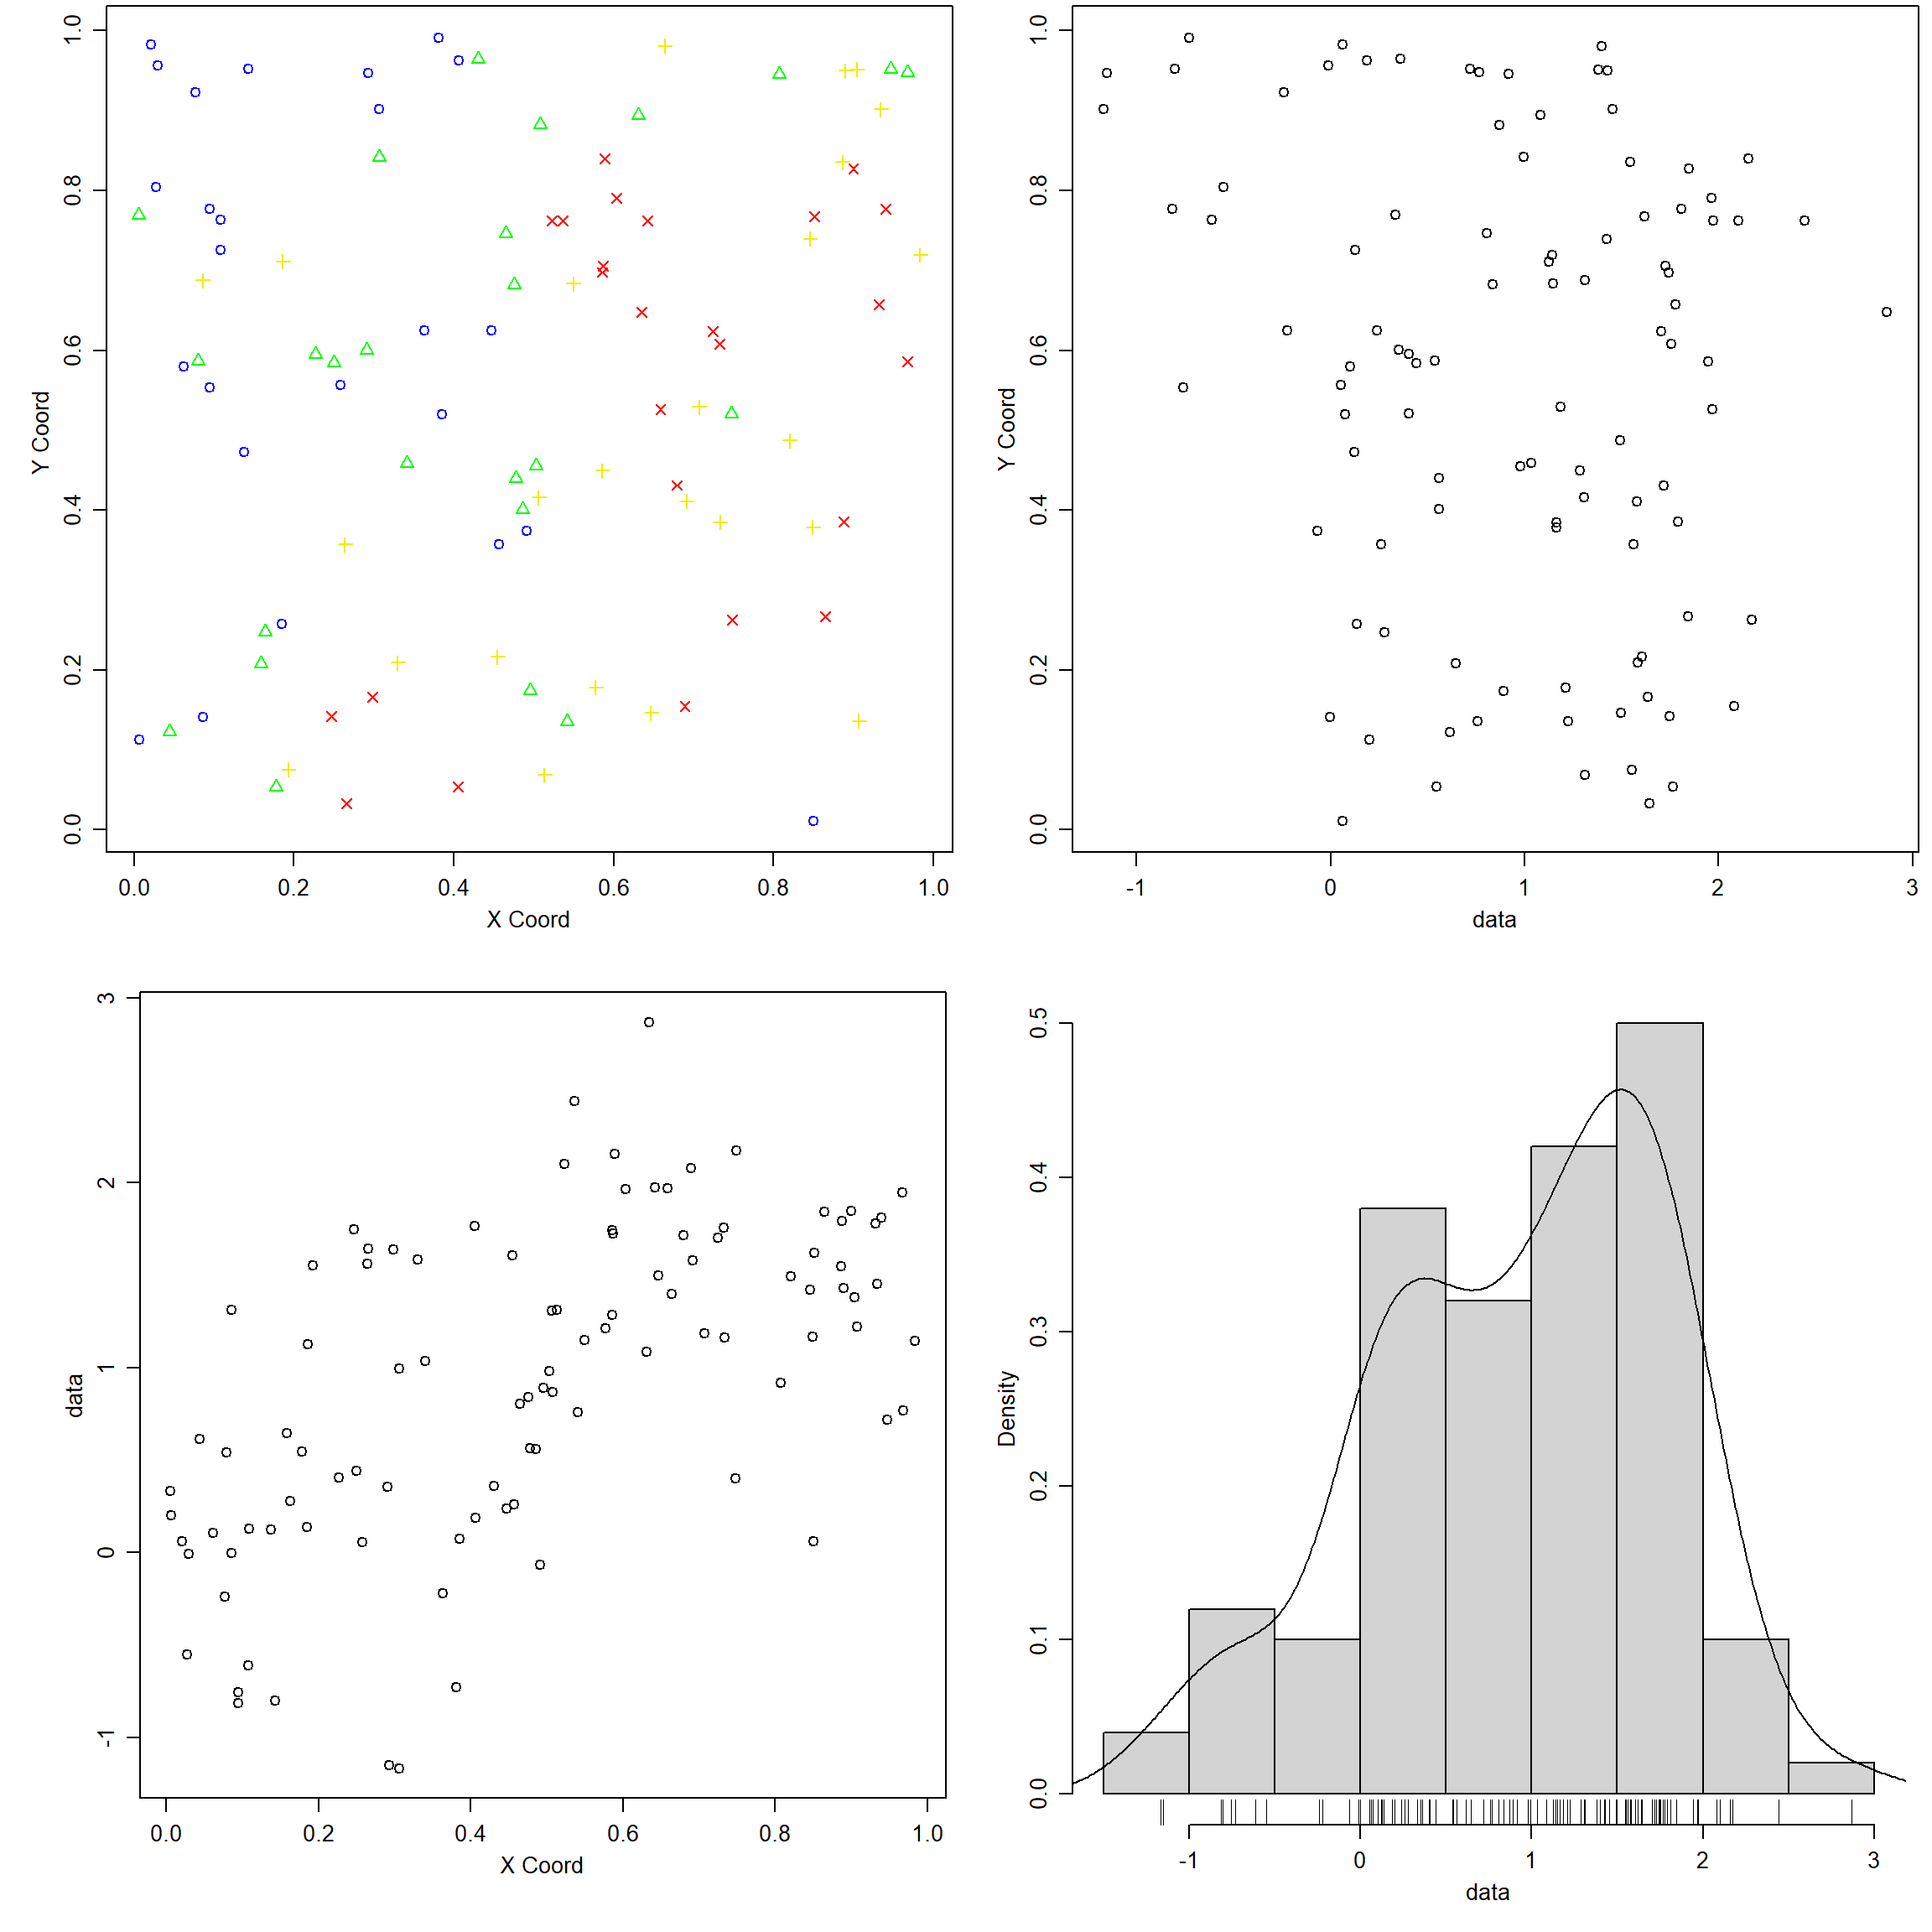
\includegraphics[width=0.9\linewidth]{12-geor_files/figure-latex/plot-s100-1} \end{center}

En el último apartado se tratará el caso general.

\hypertarget{variogramas-empuxedricos}{%
\subsection{Variogramas empíricos}\label{variogramas-empuxedricos}}

Los variogramas empíricos se calculan utilizando la función \texttt{variog}:

\begin{Shaded}
\begin{Highlighting}[]
\NormalTok{oldpar }\OtherTok{\textless{}{-}} \FunctionTok{par}\NormalTok{(}\AttributeTok{mfrow=}\FunctionTok{c}\NormalTok{(}\DecValTok{1}\NormalTok{,}\DecValTok{2}\NormalTok{)) }
\FunctionTok{plot}\NormalTok{(}\FunctionTok{variog}\NormalTok{(s100))}
\end{Highlighting}
\end{Shaded}

\begin{verbatim}
## variog: computing omnidirectional variogram
\end{verbatim}

\begin{Shaded}
\begin{Highlighting}[]
\FunctionTok{plot}\NormalTok{(}\FunctionTok{variog}\NormalTok{(s100, }\AttributeTok{max.dist =} \FloatTok{0.6}\NormalTok{))}
\end{Highlighting}
\end{Shaded}

\begin{verbatim}
## variog: computing omnidirectional variogram
\end{verbatim}

\begin{center}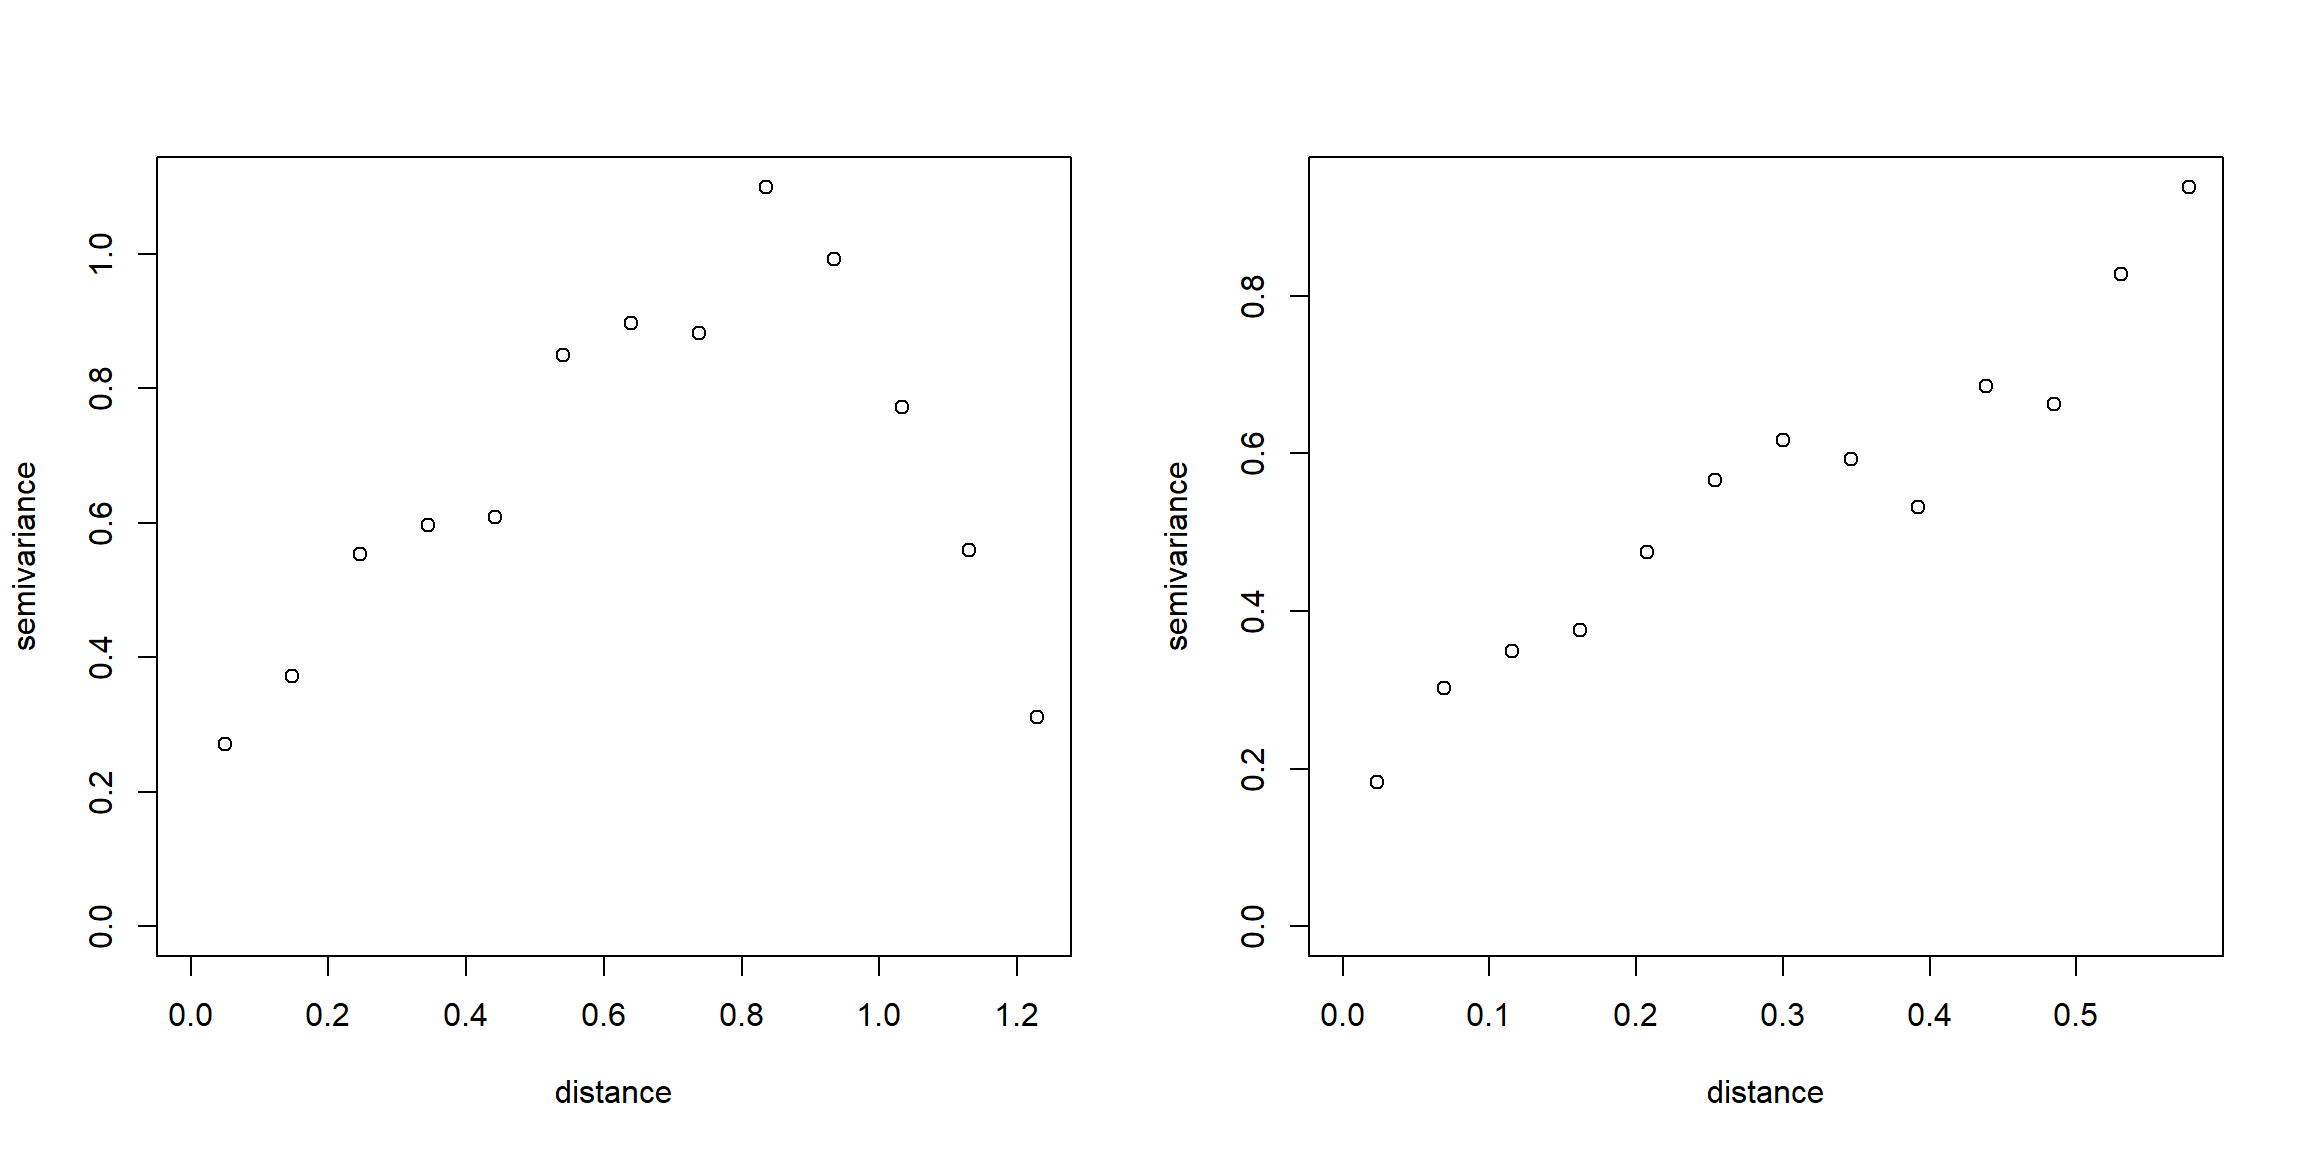
\includegraphics[width=0.9\linewidth]{12-geor_files/figure-latex/plot-variog1-1} \end{center}

\begin{Shaded}
\begin{Highlighting}[]
\FunctionTok{par}\NormalTok{(oldpar)}
\end{Highlighting}
\end{Shaded}

La recomendación es considerar solo saltos hasta la mitad de la máxima
distancia (ver `Distance summary' en resultados del sumario).

\begin{Shaded}
\begin{Highlighting}[]
\NormalTok{vario }\OtherTok{\textless{}{-}} \FunctionTok{variog}\NormalTok{(s100, }\AttributeTok{max.dist =} \FloatTok{0.6}\NormalTok{)}
\end{Highlighting}
\end{Shaded}

\begin{verbatim}
## variog: computing omnidirectional variogram
\end{verbatim}

\begin{Shaded}
\begin{Highlighting}[]
\FunctionTok{names}\NormalTok{(vario)}
\end{Highlighting}
\end{Shaded}

\begin{verbatim}
##  [1] "u"                "v"                "n"                "sd"              
##  [5] "bins.lim"         "ind.bin"          "var.mark"         "beta.ols"        
##  [9] "output.type"      "max.dist"         "estimator.type"   "n.data"          
## [13] "lambda"           "trend"            "pairs.min"        "nugget.tolerance"
## [17] "direction"        "tolerance"        "uvec"             "call"
\end{verbatim}

\begin{Shaded}
\begin{Highlighting}[]
\CommentTok{\# str(vario)}
\end{Highlighting}
\end{Shaded}

NOTA: La componente \texttt{u} contiene los saltos, \texttt{v} las estimaciones del
semivariograma (semivarianzas) y \texttt{n} el número de aportaciones.

Los resultados pueden ser nubes de puntos (semivarianzas), valores
discretizados (binned) o suavizados, dependiendo del parámetro:
\texttt{option\ =\ c("bin",\ "cloud",\ "smooth")}

\begin{Shaded}
\begin{Highlighting}[]
\CommentTok{\# Calculo de los variogramas empíricos}
\NormalTok{vario.b }\OtherTok{\textless{}{-}} \FunctionTok{variog}\NormalTok{(s100, }\AttributeTok{max.dist =} \FloatTok{0.6}\NormalTok{) }\CommentTok{\#discretizado}
\end{Highlighting}
\end{Shaded}

\begin{verbatim}
## variog: computing omnidirectional variogram
\end{verbatim}

\begin{Shaded}
\begin{Highlighting}[]
\NormalTok{vario.c }\OtherTok{\textless{}{-}} \FunctionTok{variog}\NormalTok{(s100, }\AttributeTok{max.dist=}\FloatTok{0.6}\NormalTok{, }\AttributeTok{op=}\StringTok{"cloud"}\NormalTok{)  }\CommentTok{\#nube}
\end{Highlighting}
\end{Shaded}

\begin{verbatim}
## variog: computing omnidirectional variogram
\end{verbatim}

\begin{Shaded}
\begin{Highlighting}[]
\NormalTok{vario.bc }\OtherTok{\textless{}{-}} \FunctionTok{variog}\NormalTok{(s100, }\AttributeTok{max.dist=}\FloatTok{0.6}\NormalTok{, }\AttributeTok{bin.cloud=}\ConstantTok{TRUE}\NormalTok{)  }\CommentTok{\#discretizado+nube}
\end{Highlighting}
\end{Shaded}

\begin{verbatim}
## variog: computing omnidirectional variogram
\end{verbatim}

\begin{Shaded}
\begin{Highlighting}[]
\NormalTok{vario.s }\OtherTok{\textless{}{-}} \FunctionTok{variog}\NormalTok{(s100, }\AttributeTok{max.dist=}\FloatTok{0.6}\NormalTok{, }\AttributeTok{op=}\StringTok{"sm"}\NormalTok{, }\AttributeTok{band=}\FloatTok{0.2}\NormalTok{)  }\CommentTok{\#suavizado}
\end{Highlighting}
\end{Shaded}

\begin{verbatim}
## variog: computing omnidirectional variogram
\end{verbatim}

\begin{Shaded}
\begin{Highlighting}[]
\CommentTok{\# Representación gráfica}
\NormalTok{oldpar}\OtherTok{\textless{}{-}}\FunctionTok{par}\NormalTok{(}\AttributeTok{mfrow=}\FunctionTok{c}\NormalTok{(}\DecValTok{2}\NormalTok{,}\DecValTok{2}\NormalTok{)) }\CommentTok{\# Preparar para 4 gráficos por ventana}
\FunctionTok{plot}\NormalTok{(vario.b, }\AttributeTok{main=}\StringTok{"Variograma empírico"}\NormalTok{)}
\FunctionTok{plot}\NormalTok{(vario.c, }\AttributeTok{main=}\StringTok{"Nube de puntos variograma"}\NormalTok{)}
\FunctionTok{plot}\NormalTok{(vario.bc, }\AttributeTok{bin.cloud=}\ConstantTok{TRUE}\NormalTok{, }\AttributeTok{main=}\StringTok{"Graficos de cajas"}\NormalTok{)}
\FunctionTok{title}\NormalTok{(}\StringTok{"Gráficos de cajas"}\NormalTok{) }\CommentTok{\# Corregir fallo del comando anterior}
\FunctionTok{plot}\NormalTok{(vario.s, }\AttributeTok{main=}\StringTok{"Variograma suavizado"}\NormalTok{)}
\end{Highlighting}
\end{Shaded}

\begin{center}\includegraphics[width=0.9\linewidth]{12-geor_files/figure-latex/plot-variog2-1} \end{center}

\begin{Shaded}
\begin{Highlighting}[]
\FunctionTok{par}\NormalTok{(oldpar) }\CommentTok{\# Restaurar opciones de gráficos}
\end{Highlighting}
\end{Shaded}

Si hay valores atípicos (o la distribución de los datos es asimétrica)
puede ser preferible utilizar el estimador robusto. Se puede
calcular este estimador estableciendo \texttt{estimator.type\ =\ "modulus"}:

\begin{Shaded}
\begin{Highlighting}[]
\NormalTok{varior.b }\OtherTok{\textless{}{-}} \FunctionTok{variog}\NormalTok{(s100, }\AttributeTok{estimator.type =} \StringTok{"modulus"}\NormalTok{, }\AttributeTok{max.dist=}\FloatTok{0.6}\NormalTok{)}
\end{Highlighting}
\end{Shaded}

\begin{verbatim}
## variog: computing omnidirectional variogram
\end{verbatim}

\begin{Shaded}
\begin{Highlighting}[]
\NormalTok{varior.bc }\OtherTok{\textless{}{-}} \FunctionTok{variog}\NormalTok{(s100, }\AttributeTok{estimator.type =} \StringTok{"modulus"}\NormalTok{, }\AttributeTok{max.dist=}\FloatTok{0.6}\NormalTok{, }\AttributeTok{bin.cloud=}\ConstantTok{TRUE}\NormalTok{)}
\end{Highlighting}
\end{Shaded}

\begin{verbatim}
## variog: computing omnidirectional variogram
\end{verbatim}

\begin{Shaded}
\begin{Highlighting}[]
\NormalTok{oldpar}\OtherTok{\textless{}{-}}\FunctionTok{par}\NormalTok{(}\AttributeTok{mfrow=}\FunctionTok{c}\NormalTok{(}\DecValTok{2}\NormalTok{,}\DecValTok{2}\NormalTok{)) }\CommentTok{\#Preparar para 4 gráficos por ventana}
\FunctionTok{plot}\NormalTok{(vario.b, }\AttributeTok{main=}\StringTok{"Estimador clásico"}\NormalTok{)}
\FunctionTok{plot}\NormalTok{(varior.b, }\AttributeTok{main=}\StringTok{"Estimador robusto"}\NormalTok{)}
\FunctionTok{plot}\NormalTok{(vario.bc, }\AttributeTok{bin.cloud=}\ConstantTok{TRUE}\NormalTok{)}
\FunctionTok{plot}\NormalTok{(varior.bc, }\AttributeTok{bin.cloud=}\ConstantTok{TRUE}\NormalTok{)}
\end{Highlighting}
\end{Shaded}

\begin{center}\includegraphics[width=0.9\linewidth]{12-geor_files/figure-latex/plot-variog3-1} \end{center}

\begin{Shaded}
\begin{Highlighting}[]
\FunctionTok{par}\NormalTok{(oldpar) }\CommentTok{\#Restaurar opciones de gráficos}
\end{Highlighting}
\end{Shaded}

En el caso de anisotropía, también se pueden obtener variogramas direccionales con la función
\texttt{variog} mediante los argumentos \texttt{direction} y \texttt{tolerance}. Por ejemplo,
para calcular un variograma en la dirección de 60 grados (con la
tolerancia angular por defecto de 22.5 grados):

\begin{Shaded}
\begin{Highlighting}[]
\NormalTok{vario}\FloatTok{.60} \OtherTok{\textless{}{-}} \FunctionTok{variog}\NormalTok{(s100, }\AttributeTok{max.dist =} \FloatTok{0.6}\NormalTok{, }\AttributeTok{direction =}\NormalTok{ pi}\SpecialCharTok{/}\DecValTok{3}\NormalTok{) }\CommentTok{\#variograma en la dirección de 60 grados}
\end{Highlighting}
\end{Shaded}

\begin{verbatim}
## variog: computing variogram for direction = 60 degrees (1.047 radians)
##         tolerance angle = 22.5 degrees (0.393 radians)
\end{verbatim}

Para estudiar si hay anisotropía, se pueden cálcular de forma rápida variogramas
direccionales con la función \texttt{variog4}. Por defecto calcula cuatro variogramas
direccionales, correspondientes a los ángulos 0, 45, 90 y 135 grados:

\begin{Shaded}
\begin{Highlighting}[]
\NormalTok{vario}\FloatTok{.4} \OtherTok{\textless{}{-}} \FunctionTok{variog4}\NormalTok{(s100, }\AttributeTok{max.dist =} \FloatTok{0.6}\NormalTok{)}
\end{Highlighting}
\end{Shaded}

\begin{verbatim}
## variog: computing variogram for direction = 0 degrees (0 radians)
##         tolerance angle = 22.5 degrees (0.393 radians)
## variog: computing variogram for direction = 45 degrees (0.785 radians)
##         tolerance angle = 22.5 degrees (0.393 radians)
## variog: computing variogram for direction = 90 degrees (1.571 radians)
##         tolerance angle = 22.5 degrees (0.393 radians)
## variog: computing variogram for direction = 135 degrees (2.356 radians)
##         tolerance angle = 22.5 degrees (0.393 radians)
## variog: computing omnidirectional variogram
\end{verbatim}

\begin{Shaded}
\begin{Highlighting}[]
\NormalTok{oldpar }\OtherTok{\textless{}{-}} \FunctionTok{par}\NormalTok{(}\AttributeTok{mfrow=}\FunctionTok{c}\NormalTok{(}\DecValTok{1}\NormalTok{,}\DecValTok{2}\NormalTok{))}
\FunctionTok{plot}\NormalTok{(vario}\FloatTok{.60}\NormalTok{)}
\FunctionTok{title}\NormalTok{(}\AttributeTok{main =} \FunctionTok{expression}\NormalTok{(}\FunctionTok{paste}\NormalTok{(}\StringTok{"direccional, angulo = "}\NormalTok{, }\DecValTok{60} \SpecialCharTok{*}\NormalTok{ degree)))}
\FunctionTok{plot}\NormalTok{(vario}\FloatTok{.4}\NormalTok{, }\AttributeTok{lwd =} \DecValTok{2}\NormalTok{)}
\end{Highlighting}
\end{Shaded}

\begin{center}\includegraphics[width=0.9\linewidth]{12-geor_files/figure-latex/plot-variog4-1} \end{center}

\begin{Shaded}
\begin{Highlighting}[]
\FunctionTok{par}\NormalTok{(oldpar)}
\end{Highlighting}
\end{Shaded}

\hypertarget{ajuste-de-un-modelo-de-variograma}{%
\subsection{Ajuste de un modelo de variograma}\label{ajuste-de-un-modelo-de-variograma}}

Los estimadores empíricos no pueden ser empleados en la práctica (no
verifican necesariamente las propiedades de un variograma válido), por
lo que se suele recurrir en la práctica al ajuste de un modelo válido.
Con el paquete \texttt{geoR} podemos realizar el ajuste:

\begin{enumerate}
\def\labelenumi{\arabic{enumi}.}
\item
  ``A ojo'': representando diferentes modelos sobre un variograma
  empírico (usando la función \texttt{lines.variomodel} o la función
  \texttt{eyefit}).
\item
  Por mínimos cuadrados: ajustando por mínimos cuadrados
  ordinarios (OSL) o ponderados (WLS) al variograma empírico (usando
  la función \texttt{variofit}),
\item
  Por máxima verosimilitud: estimando por máxima verosimilitud (ML) o
  máxima verosimilitud restringida (REML) los parámetros a partir de
  los datos (utilizando la función \texttt{likfit}),
\item
  Métodos bayesianos (utilizando la función \texttt{krige.bayes}).
\end{enumerate}

Ejemplo de ajuste ``a ojo'':

\begin{Shaded}
\begin{Highlighting}[]
\NormalTok{vario.b }\OtherTok{\textless{}{-}} \FunctionTok{variog}\NormalTok{(s100, }\AttributeTok{max.dist=}\FloatTok{0.6}\NormalTok{) }\CommentTok{\#discretizado}
\end{Highlighting}
\end{Shaded}

\begin{verbatim}
## variog: computing omnidirectional variogram
\end{verbatim}

\begin{Shaded}
\begin{Highlighting}[]
\NormalTok{vario.s }\OtherTok{\textless{}{-}} \FunctionTok{variog}\NormalTok{(s100, }\AttributeTok{max.dist=}\FloatTok{0.6}\NormalTok{,}\AttributeTok{option =} \StringTok{"smooth"}\NormalTok{, }\AttributeTok{kernel =} \StringTok{"normal"}\NormalTok{, }\AttributeTok{band =} \FloatTok{0.2}\NormalTok{)  }\CommentTok{\#suavizado}
\end{Highlighting}
\end{Shaded}

\begin{verbatim}
## variog: computing omnidirectional variogram
\end{verbatim}

\begin{Shaded}
\begin{Highlighting}[]
\FunctionTok{plot}\NormalTok{(vario.b)}
\FunctionTok{lines}\NormalTok{(vario.s, }\AttributeTok{type =} \StringTok{"l"}\NormalTok{, }\AttributeTok{lty =} \DecValTok{2}\NormalTok{)}

\FunctionTok{lines.variomodel}\NormalTok{(}\AttributeTok{cov.model =} \StringTok{"exp"}\NormalTok{, }\AttributeTok{cov.pars =} \FunctionTok{c}\NormalTok{(}\DecValTok{1}\NormalTok{,}\FloatTok{0.3}\NormalTok{), }\AttributeTok{nugget =} \DecValTok{0}\NormalTok{, }\AttributeTok{max.dist =} \FloatTok{0.6}\NormalTok{, }\AttributeTok{lwd =} \DecValTok{3}\NormalTok{)}
\FunctionTok{legend}\NormalTok{(}\FloatTok{0.3}\NormalTok{, }\FloatTok{0.3}\NormalTok{, }\FunctionTok{c}\NormalTok{(}\StringTok{"empirico"}\NormalTok{, }\StringTok{"suavizado"}\NormalTok{, }\StringTok{"modelo exponencial"}\NormalTok{), }\AttributeTok{lty =} \FunctionTok{c}\NormalTok{(}\DecValTok{1}\NormalTok{, }\DecValTok{2}\NormalTok{, }\DecValTok{1}\NormalTok{), }\AttributeTok{lwd =} \FunctionTok{c}\NormalTok{(}\DecValTok{1}\NormalTok{, }\DecValTok{1}\NormalTok{, }\DecValTok{3}\NormalTok{))}
\end{Highlighting}
\end{Shaded}

\begin{center}\includegraphics[width=0.7\linewidth]{12-geor_files/figure-latex/unnamed-chunk-11-1} \end{center}

Otros ajustes:

\begin{Shaded}
\begin{Highlighting}[]
\FunctionTok{plot}\NormalTok{(vario.b)}
\FunctionTok{lines.variomodel}\NormalTok{(}\AttributeTok{cov.model =} \StringTok{"exp"}\NormalTok{, }\AttributeTok{cov.pars =} \FunctionTok{c}\NormalTok{(}\FloatTok{0.9}\NormalTok{,}\FloatTok{0.3}\NormalTok{), }\AttributeTok{nug =} \FloatTok{0.1}\NormalTok{, }\AttributeTok{max.dist =} \FloatTok{0.6}\NormalTok{)}
\FunctionTok{lines.variomodel}\NormalTok{(}\AttributeTok{cov.model =} \StringTok{"mat"}\NormalTok{, }\AttributeTok{cov.pars =} \FunctionTok{c}\NormalTok{(}\FloatTok{0.85}\NormalTok{,}\FloatTok{0.2}\NormalTok{), }\AttributeTok{nug =} \FloatTok{0.1}\NormalTok{, }\AttributeTok{kappa =} \DecValTok{1}\NormalTok{, }\AttributeTok{max.dist =} \FloatTok{0.6}\NormalTok{,}\AttributeTok{lty =} \DecValTok{2}\NormalTok{)}
\FunctionTok{lines.variomodel}\NormalTok{(}\AttributeTok{cov.model =} \StringTok{"sph"}\NormalTok{, }\AttributeTok{cov.pars =} \FunctionTok{c}\NormalTok{(}\FloatTok{0.8}\NormalTok{,}\FloatTok{0.8}\NormalTok{), }\AttributeTok{nug =} \FloatTok{0.1}\NormalTok{, }\AttributeTok{max.dist =} \FloatTok{0.6}\NormalTok{, }\AttributeTok{lwd =} \DecValTok{2}\NormalTok{)}
\end{Highlighting}
\end{Shaded}

\begin{center}\includegraphics[width=0.7\linewidth]{12-geor_files/figure-latex/unnamed-chunk-12-1} \end{center}

Nota: no hace falta escribir el nombre completo de los parámetros
(basta con que no dé lugar a confusión).

En las versiones recientes de \texttt{geoR} está disponible una función para
realizar el ajuste gráficamente de forma interactiva
(cuadro de diálogo en tcl/tk):

\begin{Shaded}
\begin{Highlighting}[]
\FunctionTok{eyefit}\NormalTok{(vario.b)}
\end{Highlighting}
\end{Shaded}

Cuando se utilizan las funciones \texttt{variofit} y \texttt{likfit} para la
estimación de parámetros, el efecto pepita (nugget) puede ser estimado o
establecido a un valor fijo. Lo mismo ocurre con los parámetros de
suavidad, anisotropía y transformación de los datos. También se dispone
de opciones para incluir una tendencia. Las tendencias pueden ser
polinomios en función de las coordenadas y/o funciones lineales de otras
covariables.

Ejemplos de estimación por mínimos cuadrados (llamadas a \texttt{variofit}):

\begin{Shaded}
\begin{Highlighting}[]
\CommentTok{\#   Modelo exponencial con par ini umbral 1 y escala 0.5 (1/3 rango =1.5)}

\NormalTok{vario.ols }\OtherTok{\textless{}{-}} \FunctionTok{variofit}\NormalTok{(vario.b, }\AttributeTok{ini =} \FunctionTok{c}\NormalTok{(}\DecValTok{1}\NormalTok{, }\FloatTok{0.5}\NormalTok{), }\AttributeTok{weights =} \StringTok{"equal"}\NormalTok{)  }\CommentTok{\#ordinarios}
\end{Highlighting}
\end{Shaded}

\begin{verbatim}
## variofit: covariance model used is matern 
## variofit: weights used: equal 
## variofit: minimisation function used: optim
\end{verbatim}

\begin{Shaded}
\begin{Highlighting}[]
\NormalTok{vario.wls }\OtherTok{\textless{}{-}} \FunctionTok{variofit}\NormalTok{(vario.b, }\AttributeTok{ini =} \FunctionTok{c}\NormalTok{(}\DecValTok{1}\NormalTok{, }\FloatTok{0.5}\NormalTok{), }\AttributeTok{weights =} \StringTok{"cressie"}\NormalTok{)  }\CommentTok{\#ponderados}
\end{Highlighting}
\end{Shaded}

\begin{verbatim}
## variofit: covariance model used is matern 
## variofit: weights used: cressie 
## variofit: minimisation function used: optim
\end{verbatim}

\begin{Shaded}
\begin{Highlighting}[]
\NormalTok{vario.wls}
\end{Highlighting}
\end{Shaded}

\begin{verbatim}
## variofit: model parameters estimated by WLS (weighted least squares):
## covariance model is: matern with fixed kappa = 0.5 (exponential)
## parameter estimates:
##   tausq sigmasq     phi 
##  0.1955  2.0110  1.4811 
## Practical Range with cor=0.05 for asymptotic range: 4.437092
## 
## variofit: minimised weighted sum of squares = 31.5115
\end{verbatim}

\begin{Shaded}
\begin{Highlighting}[]
\FunctionTok{summary}\NormalTok{(vario.wls)}
\end{Highlighting}
\end{Shaded}

\begin{verbatim}
## $pmethod
## [1] "WLS (weighted least squares)"
## 
## $cov.model
## [1] "matern"
## 
## $spatial.component
##  sigmasq      phi 
## 2.010972 1.481138 
## 
## $spatial.component.extra
## kappa 
##   0.5 
## 
## $nugget.component
##     tausq 
## 0.1955322 
## 
## $fix.nugget
## [1] FALSE
## 
## $fix.kappa
## [1] TRUE
## 
## $practicalRange
## [1] 4.437092
## 
## $sum.of.squares
##   value 
## 31.5115 
## 
## $estimated.pars
##     tausq   sigmasq       phi 
## 0.1955322 2.0109718 1.4811376 
## 
## $weights
## [1] "cressie"
## 
## $call
## variofit(vario = vario.b, ini.cov.pars = c(1, 0.5), weights = "cressie")
## 
## attr(,"class")
## [1] "summary.variomodel"
\end{verbatim}

Ejemplo de estimación por máxima verosimilitud (llamada a \texttt{likfit}):

\begin{Shaded}
\begin{Highlighting}[]
\NormalTok{vario.ml }\OtherTok{\textless{}{-}} \FunctionTok{likfit}\NormalTok{(s100, }\AttributeTok{ini =} \FunctionTok{c}\NormalTok{(}\DecValTok{1}\NormalTok{, }\FloatTok{0.5}\NormalTok{)) }\CommentTok{\#Modelo exponencial con par ini umbral y escala (1/3 rango)}
\end{Highlighting}
\end{Shaded}

\begin{verbatim}
## ---------------------------------------------------------------
## likfit: likelihood maximisation using the function optim.
## likfit: Use control() to pass additional
##          arguments for the maximisation function.
##         For further details see documentation for optim.
## likfit: It is highly advisable to run this function several
##         times with different initial values for the parameters.
## likfit: WARNING: This step can be time demanding!
## ---------------------------------------------------------------
## likfit: end of numerical maximisation.
\end{verbatim}

\begin{Shaded}
\begin{Highlighting}[]
\NormalTok{vario.ml}
\end{Highlighting}
\end{Shaded}

\begin{verbatim}
## likfit: estimated model parameters:
##     beta    tausq  sigmasq      phi 
## "0.7766" "0.0000" "0.7517" "0.1827" 
## Practical Range with cor=0.05 for asymptotic range: 0.547383
## 
## likfit: maximised log-likelihood = -83.57
\end{verbatim}

\begin{Shaded}
\begin{Highlighting}[]
\FunctionTok{summary}\NormalTok{(vario.ml)}
\end{Highlighting}
\end{Shaded}

\begin{verbatim}
## Summary of the parameter estimation
## -----------------------------------
## Estimation method: maximum likelihood 
## 
## Parameters of the mean component (trend):
##   beta 
## 0.7766 
## 
## Parameters of the spatial component:
##    correlation function: exponential
##       (estimated) variance parameter sigmasq (partial sill) =  0.7517
##       (estimated) cor. fct. parameter phi (range parameter)  =  0.1827
##    anisotropy parameters:
##       (fixed) anisotropy angle = 0  ( 0 degrees )
##       (fixed) anisotropy ratio = 1
## 
## Parameter of the error component:
##       (estimated) nugget =  0
## 
## Transformation parameter:
##       (fixed) Box-Cox parameter = 1 (no transformation)
## 
## Practical Range with cor=0.05 for asymptotic range: 0.547383
## 
## Maximised Likelihood:
##    log.L n.params      AIC      BIC 
## "-83.57"      "4"  "175.1"  "185.6" 
## 
## non spatial model:
##    log.L n.params      AIC      BIC 
## "-125.8"      "2"  "255.6"  "260.8" 
## 
## Call:
## likfit(geodata = s100, ini.cov.pars = c(1, 0.5))
\end{verbatim}

Ejemplo de estimación por máxima verosimilitud restringida (opción de
\texttt{likfit}):

\begin{Shaded}
\begin{Highlighting}[]
\NormalTok{vario.reml }\OtherTok{\textless{}{-}} \FunctionTok{likfit}\NormalTok{(s100, }\AttributeTok{ini =} \FunctionTok{c}\NormalTok{(}\DecValTok{1}\NormalTok{, }\FloatTok{0.5}\NormalTok{), }\AttributeTok{lik.method =} \StringTok{"RML"}\NormalTok{)}
\end{Highlighting}
\end{Shaded}

\begin{verbatim}
## ---------------------------------------------------------------
## likfit: likelihood maximisation using the function optim.
## likfit: Use control() to pass additional
##          arguments for the maximisation function.
##         For further details see documentation for optim.
## likfit: It is highly advisable to run this function several
##         times with different initial values for the parameters.
## likfit: WARNING: This step can be time demanding!
## ---------------------------------------------------------------
## likfit: end of numerical maximisation.
\end{verbatim}

\begin{Shaded}
\begin{Highlighting}[]
\FunctionTok{summary}\NormalTok{(vario.reml)}
\end{Highlighting}
\end{Shaded}

\begin{verbatim}
## Summary of the parameter estimation
## -----------------------------------
## Estimation method: restricted maximum likelihood 
## 
## Parameters of the mean component (trend):
##   beta 
## 0.7478 
## 
## Parameters of the spatial component:
##    correlation function: exponential
##       (estimated) variance parameter sigmasq (partial sill) =  0.8473
##       (estimated) cor. fct. parameter phi (range parameter)  =  0.2102
##    anisotropy parameters:
##       (fixed) anisotropy angle = 0  ( 0 degrees )
##       (fixed) anisotropy ratio = 1
## 
## Parameter of the error component:
##       (estimated) nugget =  0
## 
## Transformation parameter:
##       (fixed) Box-Cox parameter = 1 (no transformation)
## 
## Practical Range with cor=0.05 for asymptotic range: 0.6296295
## 
## Maximised Likelihood:
##    log.L n.params      AIC      BIC 
## "-81.53"      "4"  "171.1"  "181.5" 
## 
## non spatial model:
##    log.L n.params      AIC      BIC 
## "-125.1"      "2"  "254.1"  "259.3" 
## 
## Call:
## likfit(geodata = s100, ini.cov.pars = c(1, 0.5), lik.method = "RML")
\end{verbatim}

\textbf{NOTAS}:

\begin{itemize}
\item
  Para fijar el nugget a un valor p.e. 0.15 añadir las opciones:
  \texttt{fix.nugget\ =\ TRUE,\ nugget\ =\ 0.15}.
\item
  Se puede tener en cuenta anisotropía geométrica en los modelos de
  variograma a partir de los parámetros \texttt{psiA} (ángulo, en radianes,
  de la dirección de mayor dependencia espacial i.e.~con el
  máximo rango) y \texttt{psiR} (relación, mayor o igual que 1, entre los
  rangos máximo y mínimo). Se pueden fijar a distintos valores o
  estimarlos incluyendo las opciones \texttt{fix.psiA\ =\ FALSE} y \texttt{fix.psiR\ =\ \ \ \ \ FALSE} en las llamadas a las rutinas de ajuste.)
\end{itemize}

Representación gráfica junto al estimador empírico:

\begin{Shaded}
\begin{Highlighting}[]
\FunctionTok{plot}\NormalTok{(vario.b, }\AttributeTok{main =} \StringTok{"Estimador empírico y modelos ajustados"}\NormalTok{)}
\FunctionTok{lines}\NormalTok{(vario.ml, }\AttributeTok{max.dist =} \FloatTok{0.6}\NormalTok{)}
\FunctionTok{lines}\NormalTok{(vario.reml, }\AttributeTok{lwd =} \DecValTok{2}\NormalTok{, }\AttributeTok{max.dist =} \FloatTok{0.6}\NormalTok{)}
\FunctionTok{lines}\NormalTok{(vario.ols, }\AttributeTok{lty =} \DecValTok{2}\NormalTok{, }\AttributeTok{max.dist =} \FloatTok{0.6}\NormalTok{)}
\FunctionTok{lines}\NormalTok{(vario.wls, }\AttributeTok{lty =} \DecValTok{2}\NormalTok{, }\AttributeTok{lwd =} \DecValTok{2}\NormalTok{, }\AttributeTok{max.dist =} \FloatTok{0.6}\NormalTok{)}
\FunctionTok{legend}\NormalTok{(}\FloatTok{0.3}\NormalTok{, }\FloatTok{0.3}\NormalTok{, }\AttributeTok{legend =} \FunctionTok{c}\NormalTok{(}\StringTok{"ML"}\NormalTok{, }\StringTok{"REML"}\NormalTok{, }\StringTok{"OLS"}\NormalTok{, }\StringTok{"WLS"}\NormalTok{), }\AttributeTok{lty =} \FunctionTok{c}\NormalTok{(}\DecValTok{1}\NormalTok{, }\DecValTok{1}\NormalTok{, }\DecValTok{2}\NormalTok{, }\DecValTok{2}\NormalTok{), }\AttributeTok{lwd =} \FunctionTok{c}\NormalTok{(}\DecValTok{1}\NormalTok{, }\DecValTok{2}\NormalTok{,}\DecValTok{1}\NormalTok{, }\DecValTok{2}\NormalTok{)) }
\end{Highlighting}
\end{Shaded}

\begin{center}\includegraphics[width=0.7\linewidth]{12-geor_files/figure-latex/unnamed-chunk-17-1} \end{center}

\hypertarget{inferencia-sobre-el-variograma}{%
\subsection{Inferencia sobre el variograma}\label{inferencia-sobre-el-variograma}}

Se pueden obtener dos tipos de envolventes (envelopes, i.e.~valores
máximos y mínimos aproximados) del variograma empírico mediante
simulación:

\begin{itemize}
\item
  Bajo la hipótesis de que no hay correlación espacial (obtenidos por
  permutaciones aleatorias de los datos sobre las posiciones
  espaciales), para estudiar si hay una dependencia
  espacial ``significativa''.
\item
  Bajo un modelo de variograma, para ilustrar la variabilidad del
  variograma empírico.
\end{itemize}

\begin{Shaded}
\begin{Highlighting}[]
\NormalTok{env.indep }\OtherTok{\textless{}{-}} \FunctionTok{variog.mc.env}\NormalTok{(s100, }\AttributeTok{obj.var =}\NormalTok{ vario.b)}
\end{Highlighting}
\end{Shaded}

\begin{verbatim}
## variog.env: generating 99 simulations by permutating data values
## variog.env: computing the empirical variogram for the 99 simulations
## variog.env: computing the envelops
\end{verbatim}

\begin{Shaded}
\begin{Highlighting}[]
\NormalTok{env.model }\OtherTok{\textless{}{-}} \FunctionTok{variog.model.env}\NormalTok{(s100, }\AttributeTok{obj.var =}\NormalTok{ vario.b, }\AttributeTok{model =}\NormalTok{ vario.wls)}
\end{Highlighting}
\end{Shaded}

\begin{verbatim}
## variog.env: generating 99 simulations (with  100 points each) using the function grf
## variog.env: adding the mean or trend
## variog.env: computing the empirical variogram for the 99 simulations
## variog.env: computing the envelops
\end{verbatim}

\begin{Shaded}
\begin{Highlighting}[]
\NormalTok{oldpar }\OtherTok{\textless{}{-}} \FunctionTok{par}\NormalTok{(}\AttributeTok{mfrow =} \FunctionTok{c}\NormalTok{(}\DecValTok{1}\NormalTok{, }\DecValTok{2}\NormalTok{))}
\FunctionTok{plot}\NormalTok{(vario.b, }\AttributeTok{envelope =}\NormalTok{ env.indep)}
\FunctionTok{plot}\NormalTok{(vario.b, }\AttributeTok{envelope =}\NormalTok{ env.model)}
\FunctionTok{lines}\NormalTok{(vario.wls, }\AttributeTok{lty =} \DecValTok{2}\NormalTok{, }\AttributeTok{lwd =} \DecValTok{2}\NormalTok{, }\AttributeTok{max.dist =} \FloatTok{0.6}\NormalTok{)}
\end{Highlighting}
\end{Shaded}

\begin{center}\includegraphics[width=0.9\linewidth]{12-geor_files/figure-latex/plot-variog-env-1} \end{center}

\begin{Shaded}
\begin{Highlighting}[]
\FunctionTok{par}\NormalTok{(oldpar)     }
\end{Highlighting}
\end{Shaded}

Para estudiar si hay una dependencia espacial ``significativa'' se puede
emplear también la rutina \texttt{sm.variogram} del paquete \texttt{sm}.
Estableciendo \texttt{model\ =\ "independent"}
devuelve un p-valor para contrastar la hipótesis nula de independencia
(i.e.~se acepta que hay una dependencia espacial si \(p \leq \alpha = 0.05\))
y un gráfico en el que se muestra el estimador empírico robusto, un estimador
suavizado y una región de confianza para el variograma suponiendo que el
proceso es independiente (i.e.~consideraríamos que hay dependencia
espacial si el variograma suavizado no está contenido en esa región).

\begin{Shaded}
\begin{Highlighting}[]
\FunctionTok{library}\NormalTok{(sm)}
\end{Highlighting}
\end{Shaded}

\begin{verbatim}
## Package 'sm', version 2.2-5.7: type help(sm) for summary information
\end{verbatim}

\begin{Shaded}
\begin{Highlighting}[]
\FunctionTok{sm.variogram}\NormalTok{(s100}\SpecialCharTok{$}\NormalTok{coords, s100}\SpecialCharTok{$}\NormalTok{data, }\AttributeTok{model =} \StringTok{"independent"}\NormalTok{)}
\end{Highlighting}
\end{Shaded}

\begin{verbatim}
## Test of spatial independence: p =  0.024
\end{verbatim}

\begin{center}\includegraphics[width=0.7\linewidth]{12-geor_files/figure-latex/unnamed-chunk-18-1} \end{center}

\textbf{Nota}: Se puede realizar contrastes adicionales estableciendo el parámetro \texttt{model}
a \texttt{"isotropic"} o \texttt{"stationary"}.

\hypertarget{estimaciuxf3n-del-variograma-en-procesos-no-estacionarios}{%
\subsection{Estimación del variograma en procesos no estacionarios}\label{estimaciuxf3n-del-variograma-en-procesos-no-estacionarios}}

Cuando el proceso no es estacionario (no se puede emplear directamente los
estimadores empíricos) hay que eliminar la tendencia para estimar el variograma:

\begin{Shaded}
\begin{Highlighting}[]
\NormalTok{oldpar }\OtherTok{\textless{}{-}} \FunctionTok{par}\NormalTok{(}\AttributeTok{mfrow=}\FunctionTok{c}\NormalTok{(}\DecValTok{1}\NormalTok{,}\DecValTok{2}\NormalTok{)) }
\FunctionTok{plot}\NormalTok{(}\FunctionTok{variog}\NormalTok{(wolfcamp, }\AttributeTok{max.dist =} \DecValTok{200}\NormalTok{)) }\CommentTok{\# Supone que el proceso es estacionario}
\end{Highlighting}
\end{Shaded}

\begin{verbatim}
## variog: computing omnidirectional variogram
\end{verbatim}

\begin{Shaded}
\begin{Highlighting}[]
\FunctionTok{plot}\NormalTok{(}\FunctionTok{variog}\NormalTok{(wolfcamp, }\AttributeTok{trend =} \SpecialCharTok{\textasciitilde{}}\NormalTok{coords, }\AttributeTok{max.dist =} \DecValTok{200}\NormalTok{)) }\CommentTok{\# Asume una tendencia lineal en las coordenadas}
\end{Highlighting}
\end{Shaded}

\begin{verbatim}
## variog: computing omnidirectional variogram
\end{verbatim}

\begin{center}\includegraphics[width=0.8\linewidth]{12-geor_files/figure-latex/plot-variog-wolf-1} \end{center}

\begin{Shaded}
\begin{Highlighting}[]
\FunctionTok{par}\NormalTok{(oldpar)}
\end{Highlighting}
\end{Shaded}

\hypertarget{predicciuxf3n-espacial-kriging}{%
\section{Predicción espacial (kriging)}\label{predicciuxf3n-espacial-kriging}}

El paquete \texttt{geoR} dispone de opciones para los métodos kriging
tradicionales, que dependiendo de las suposiciones acerca de la función
de tendencia se clasifican en:

\begin{itemize}
\item
  \emph{Kriging simple} (\textbf{KS}): media conocida
\item
  \emph{Kriging ordinario} (\textbf{KO}): se supone que la media es constante
  y desconocida.
\item
  \emph{Kriging universal} (\textbf{KU}): también denominado kriging con modelo de
  tendencia, se supone que la media es una combinación
  lineal (desconocida) de las coordenadas o de otras
  variables explicativas.
\end{itemize}

Existen también opciones adicionales para kriging trans-normal (con
transformaciones Box-Cox para aproximarse a la normalidad y
transformación de nuevo de resultados a la escala original manteniendo
insesgadez). También admite modelos de variograma geométricamente
anisotrópicos.

Para obtener una rejilla discreta de predicción puede ser de utilidad la
función \texttt{expand.grid}:

\begin{Shaded}
\begin{Highlighting}[]
\CommentTok{\# Rejilla regular 51x51 en cuadrado unidad}
\NormalTok{xx }\OtherTok{\textless{}{-}} \FunctionTok{seq}\NormalTok{(}\DecValTok{0}\NormalTok{, }\DecValTok{1}\NormalTok{, }\AttributeTok{l =} \DecValTok{51}\NormalTok{)}
\NormalTok{yy }\OtherTok{\textless{}{-}} \FunctionTok{seq}\NormalTok{(}\DecValTok{0}\NormalTok{, }\DecValTok{1}\NormalTok{, }\AttributeTok{l =} \DecValTok{51}\NormalTok{)}
\NormalTok{pred.grid }\OtherTok{\textless{}{-}} \FunctionTok{expand.grid}\NormalTok{(}\AttributeTok{x =}\NormalTok{ xx, }\AttributeTok{y =}\NormalTok{ yy) }
\FunctionTok{plot}\NormalTok{(s100}\SpecialCharTok{$}\NormalTok{coords, }\AttributeTok{pch =} \DecValTok{20}\NormalTok{, }\AttributeTok{asp =} \DecValTok{1}\NormalTok{)}
\FunctionTok{points}\NormalTok{(pred.grid, }\AttributeTok{pch =} \DecValTok{3}\NormalTok{, }\AttributeTok{cex =} \FloatTok{0.2}\NormalTok{)}
\end{Highlighting}
\end{Shaded}

\begin{center}\includegraphics[width=0.7\linewidth]{12-geor_files/figure-latex/unnamed-chunk-19-1} \end{center}

El comando para realizar kriging ordinario con variograma \texttt{vario.wls}
sería:

\begin{Shaded}
\begin{Highlighting}[]
\NormalTok{ko.wls }\OtherTok{\textless{}{-}} \FunctionTok{krige.conv}\NormalTok{(s100, }\AttributeTok{loc =}\NormalTok{ pred.grid, }\AttributeTok{krige =} \FunctionTok{krige.control}\NormalTok{(}\AttributeTok{obj.m =}\NormalTok{ vario.wls))}
\end{Highlighting}
\end{Shaded}

\begin{verbatim}
## krige.conv: model with constant mean
## krige.conv: Kriging performed using global neighbourhood
\end{verbatim}

El resultado es una lista incluyendo predicciones (\texttt{ko.wls\$predict}) y
varianzas kriging (\texttt{ko.wls\$krige.var}):

\begin{Shaded}
\begin{Highlighting}[]
\FunctionTok{names}\NormalTok{(ko.wls)}
\end{Highlighting}
\end{Shaded}

\begin{verbatim}
## [1] "predict"      "krige.var"    "beta.est"     "distribution" "message"     
## [6] "call"
\end{verbatim}

Para ver todas las opciones de kriging disponibles ejecutar
\texttt{?krige.control}. Para kriging con vecindario local (archivos de datos
grandes) se puede utilizar la función \texttt{ksline}.

Para representar las superficies se podría utilizar la función \texttt{image()},
aunque la última versión del método \texttt{image.kriging()} puede fallar al añadir
elementos (por lo menos en RMarkdown; tampoco es compatible con \texttt{par(mfrow)}):

\begin{Shaded}
\begin{Highlighting}[]
\CommentTok{\# oldpar \textless{}{-} par(mfrow = c(1, 2)) }
\CommentTok{\# image.kriging no es compatible con mfrow en últimas versiones}
\FunctionTok{image}\NormalTok{(ko.wls, }\AttributeTok{coords.data=}\NormalTok{s100}\SpecialCharTok{$}\NormalTok{coords, }\AttributeTok{main =} \StringTok{"Superficie de predicciones"}\NormalTok{)}
\FunctionTok{contour}\NormalTok{(ko.wls, }\AttributeTok{add =} \ConstantTok{TRUE}\NormalTok{) }\CommentTok{\#añadir gráfico de contorno}
\end{Highlighting}
\end{Shaded}

\begin{center}\includegraphics[width=0.7\linewidth]{12-geor_files/figure-latex/unnamed-chunk-22-1} \end{center}

\begin{Shaded}
\begin{Highlighting}[]
\FunctionTok{image}\NormalTok{(ko.wls, }\AttributeTok{coords.data=}\NormalTok{s100}\SpecialCharTok{$}\NormalTok{coords, }\AttributeTok{values =} \FunctionTok{sqrt}\NormalTok{(ko.wls}\SpecialCharTok{$}\NormalTok{krige.var), }\AttributeTok{main =} \StringTok{"Superficie de err. std. kriging"}\NormalTok{) }
\FunctionTok{contour}\NormalTok{(ko.wls, }\AttributeTok{values =} \FunctionTok{sqrt}\NormalTok{(ko.wls}\SpecialCharTok{$}\NormalTok{krige.var), }\AttributeTok{add =} \ConstantTok{TRUE}\NormalTok{)}
\end{Highlighting}
\end{Shaded}

\begin{center}\includegraphics[width=0.7\linewidth]{12-geor_files/figure-latex/unnamed-chunk-22-2} \end{center}

\begin{Shaded}
\begin{Highlighting}[]
\CommentTok{\# par(oldpar)}
\end{Highlighting}
\end{Shaded}

Otras opciones:

\begin{Shaded}
\begin{Highlighting}[]
\FunctionTok{contour}\NormalTok{(ko.wls,}\AttributeTok{filled =} \ConstantTok{TRUE}\NormalTok{)}
\end{Highlighting}
\end{Shaded}

\begin{center}\includegraphics[width=0.7\linewidth]{12-geor_files/figure-latex/unnamed-chunk-23-1} \end{center}

\begin{Shaded}
\begin{Highlighting}[]
\NormalTok{fcol }\OtherTok{\textless{}{-}} \FunctionTok{topo.colors}\NormalTok{(}\DecValTok{10}\NormalTok{)[}\FunctionTok{cut}\NormalTok{(}\FunctionTok{matrix}\NormalTok{(ko.wls}\SpecialCharTok{$}\NormalTok{pred,}\AttributeTok{nrow=}\DecValTok{51}\NormalTok{,}\AttributeTok{ncol=}\DecValTok{51}\NormalTok{)[}\SpecialCharTok{{-}}\DecValTok{1}\NormalTok{,}\SpecialCharTok{{-}}\DecValTok{1}\NormalTok{],}\DecValTok{10}\NormalTok{,}\AttributeTok{include.lowest=}\ConstantTok{TRUE}\NormalTok{)]}
\FunctionTok{persp}\NormalTok{(ko.wls, }\AttributeTok{theta=}\SpecialCharTok{{-}}\DecValTok{60}\NormalTok{, }\AttributeTok{phi=}\DecValTok{40}\NormalTok{, }\AttributeTok{col=}\NormalTok{fcol)}
\end{Highlighting}
\end{Shaded}

\begin{center}\includegraphics[width=0.7\linewidth]{12-geor_files/figure-latex/unnamed-chunk-23-2} \end{center}

\begin{Shaded}
\begin{Highlighting}[]
\ControlFlowTok{if}\NormalTok{(}\SpecialCharTok{!}\FunctionTok{require}\NormalTok{(plot3D)) }
  \FunctionTok{stop}\NormalTok{(}\StringTok{\textquotesingle{}Required pakage \textasciigrave{}plot3D\textasciigrave{} not installed.\textquotesingle{}}\NormalTok{) }\CommentTok{\# install.packages(\textquotesingle{}plot3D\textquotesingle{})}
\end{Highlighting}
\end{Shaded}

\begin{verbatim}
## Loading required package: plot3D
\end{verbatim}

\begin{Shaded}
\begin{Highlighting}[]
\FunctionTok{persp3D}\NormalTok{(xx, yy, }\FunctionTok{matrix}\NormalTok{(ko.wls}\SpecialCharTok{$}\NormalTok{predict, }\AttributeTok{nrow =} \FunctionTok{length}\NormalTok{(xx)), }\AttributeTok{theta=}\SpecialCharTok{{-}}\DecValTok{60}\NormalTok{, }\AttributeTok{phi=}\DecValTok{40}\NormalTok{)}
\end{Highlighting}
\end{Shaded}

\begin{center}\includegraphics[width=0.7\linewidth]{12-geor_files/figure-latex/unnamed-chunk-23-3} \end{center}

\begin{Shaded}
\begin{Highlighting}[]
\ControlFlowTok{if}\NormalTok{(}\SpecialCharTok{!}\FunctionTok{require}\NormalTok{(npsp)) \{}
  \FunctionTok{cat}\NormalTok{(}\StringTok{"Required pakage \textasciigrave{}npsp\textasciigrave{} not installed!}\SpecialCharTok{\textbackslash{}n}\StringTok{"}\NormalTok{)   }
  \FunctionTok{cat}\NormalTok{(}\StringTok{"On windows, run \textasciigrave{}install.packages(\textquotesingle{}https://github.com/rubenfcasal/npsp/releases/download/v0.7{-}8/npsp\_0.7{-}8.zip\textquotesingle{}, repos = NULL)\textasciigrave{}}\SpecialCharTok{\textbackslash{}n}\StringTok{"}\NormalTok{)  }
\NormalTok{\} }\ControlFlowTok{else}  
  \FunctionTok{spersp}\NormalTok{(xx, yy, ko.wls}\SpecialCharTok{$}\NormalTok{predict, }\AttributeTok{theta=}\SpecialCharTok{{-}}\DecValTok{60}\NormalTok{, }\AttributeTok{phi=}\DecValTok{40}\NormalTok{)}
\end{Highlighting}
\end{Shaded}

\begin{verbatim}
## Loading required package: npsp
\end{verbatim}

\begin{verbatim}
##  Package npsp: Nonparametric Spatial Statistics,
##  version 0.7-9 (built on 2021-05-17).
##  Copyright (C) R. Fernandez-Casal 2012-2021.
##  Type `help(npsp)` for an overview of the package or
##  visit https://rubenfcasal.github.io/npsp.
\end{verbatim}

\begin{verbatim}
## 
## Attaching package: 'npsp'
\end{verbatim}

\begin{verbatim}
## The following object is masked from 'package:sm':
## 
##     binning
\end{verbatim}

\begin{center}\includegraphics[width=0.7\linewidth]{12-geor_files/figure-latex/unnamed-chunk-23-4} \end{center}

\hypertarget{validaciuxf3n-cruzada}{%
\subsection{Validación cruzada}\label{validaciuxf3n-cruzada}}

Para verificar si un modelo (de tendencia y variograma) describe adecuadamente
la variabilidad espacial de los datos (p.e. para comparar modelos), se emplea
normalmente la técnica de validación cruzada, función \texttt{xvalid} en \texttt{geoR}.
Por defecto la validación se realiza sobre los datos eliminando cada
observación (y utilizando las restantes para predecir), aunque se puede
utilizar un conjunto diferente de posiciones (o de datos) mediante el
argumento \texttt{location.xvalid} (y \texttt{data.xvalid}).

En el caso de procesos estacionarios permitiría diagnosticar si el modelo de
variograma describe adecuadamente la dependencia espacial de los datos:

\begin{Shaded}
\begin{Highlighting}[]
\NormalTok{xv.wls }\OtherTok{\textless{}{-}} \FunctionTok{xvalid}\NormalTok{(s100, }\AttributeTok{model =}\NormalTok{ vario.wls)}
\end{Highlighting}
\end{Shaded}

\begin{verbatim}
## xvalid: number of data locations       = 100
## xvalid: number of validation locations = 100
## xvalid: performing cross-validation at location ... 1, 2, 3, 4, 5, 6, 7, 8, 9, 10, 11, 12, 13, 14, 15, 16, 17, 18, 19, 20, 21, 22, 23, 24, 25, 26, 27, 28, 29, 30, 31, 32, 33, 34, 35, 36, 37, 38, 39, 40, 41, 42, 43, 44, 45, 46, 47, 48, 49, 50, 51, 52, 53, 54, 55, 56, 57, 58, 59, 60, 61, 62, 63, 64, 65, 66, 67, 68, 69, 70, 71, 72, 73, 74, 75, 76, 77, 78, 79, 80, 81, 82, 83, 84, 85, 86, 87, 88, 89, 90, 91, 92, 93, 94, 95, 96, 97, 98, 99, 100, 
## xvalid: end of cross-validation
\end{verbatim}

\begin{Shaded}
\begin{Highlighting}[]
\FunctionTok{summary}\NormalTok{(xv.wls)}
\end{Highlighting}
\end{Shaded}

\begin{verbatim}
##                 Min.    1st Qu.     Median         Mean   3rd Qu.     Max.
## errors     -1.429944 -0.4017821 0.04881742 0.0008450629 0.3359677 1.319640
## std.errors -2.110654 -0.7048560 0.07804159 0.0011568059 0.5922810 2.228054
##                   sd
## errors     0.5299818
## std.errors 0.9190753
\end{verbatim}

\begin{Shaded}
\begin{Highlighting}[]
\NormalTok{xv.reml }\OtherTok{\textless{}{-}} \FunctionTok{xvalid}\NormalTok{(s100, }\AttributeTok{model =}\NormalTok{ vario.reml)}
\end{Highlighting}
\end{Shaded}

\begin{verbatim}
## xvalid: number of data locations       = 100
## xvalid: number of validation locations = 100
## xvalid: performing cross-validation at location ... 1, 2, 3, 4, 5, 6, 7, 8, 9, 10, 11, 12, 13, 14, 15, 16, 17, 18, 19, 20, 21, 22, 23, 24, 25, 26, 27, 28, 29, 30, 31, 32, 33, 34, 35, 36, 37, 38, 39, 40, 41, 42, 43, 44, 45, 46, 47, 48, 49, 50, 51, 52, 53, 54, 55, 56, 57, 58, 59, 60, 61, 62, 63, 64, 65, 66, 67, 68, 69, 70, 71, 72, 73, 74, 75, 76, 77, 78, 79, 80, 81, 82, 83, 84, 85, 86, 87, 88, 89, 90, 91, 92, 93, 94, 95, 96, 97, 98, 99, 100, 
## xvalid: end of cross-validation
\end{verbatim}

\begin{Shaded}
\begin{Highlighting}[]
\FunctionTok{summary}\NormalTok{(xv.reml)}
\end{Highlighting}
\end{Shaded}

\begin{verbatim}
##                 Min.    1st Qu.     Median        Mean   3rd Qu.     Max.
## errors     -1.178020 -0.3109277 0.02326020 0.011894019 0.2631596 1.521489
## std.errors -2.419106 -0.7304294 0.07954355 0.009241635 0.5802049 2.690047
##                   sd
## errors     0.4813133
## std.errors 0.9906166
\end{verbatim}

Por defecto la función \texttt{plot} (\texttt{plot.xvalid}) muestra 10 gráficos
diferentes (para más información ejecutar \texttt{?plot.xvalid}), a grosso modo
los cinco primeros se corresponden con residuos simples (valores
observados menos predicciones) y los siguientes con residuos
estandarizados (dividiendo por la raíz cuadrada de la varianza de
predicción).

\begin{Shaded}
\begin{Highlighting}[]
\NormalTok{oldpar }\OtherTok{\textless{}{-}} \FunctionTok{par}\NormalTok{(}\AttributeTok{mfrow =} \FunctionTok{c}\NormalTok{(}\DecValTok{2}\NormalTok{, }\DecValTok{5}\NormalTok{), }\AttributeTok{mar =} \FunctionTok{c}\NormalTok{(}\AttributeTok{bottom =} \FloatTok{4.5}\NormalTok{, }\AttributeTok{left =} \DecValTok{4}\NormalTok{, }\AttributeTok{top =} \DecValTok{2}\NormalTok{, }\AttributeTok{right =} \DecValTok{2}\NormalTok{))}
\FunctionTok{plot}\NormalTok{(xv.wls, }\AttributeTok{ask =} \ConstantTok{FALSE}\NormalTok{)}
\end{Highlighting}
\end{Shaded}

\begin{center}\includegraphics[width=1\linewidth]{12-geor_files/figure-latex/plot-xvalid-1} \end{center}

\begin{Shaded}
\begin{Highlighting}[]
\FunctionTok{par}\NormalTok{(oldpar)}

\CommentTok{\# plot(xv.reml)}
\end{Highlighting}
\end{Shaded}

\textbf{NOTA}: Para re-estimar los parámetros del modelo cada vez que se
elimina una observación (i.e.~validar el procedimiento de estimación)
añadir la opción \texttt{reest\ =\ TRUE} (puede requerir mucho tiempo de
computación).

\hypertarget{referencias}{%
\chapter*{Referencias}\label{referencias}}
\addcontentsline{toc}{chapter}{Referencias}

\textbf{Bibliografía básica}

Bivand, R.S., Pebesma, E.J. y Gómez-Rubio, V. (2008). \emph{Applied Spatial Data Analysis with R}. Springer.

Diggle, P. y Ribeiro, P.J. (2007). \emph{Model-based Geostatistics}. Springer.

Schabenberger, O. y Gotway, C.A. (2005). \emph{Statistical Methods for Spatial Data Analysis}. Chapman and Hall.

\textbf{Bibliografía complementaria}

Chilès, J.P. y P. Delfiner (2012). \emph{Geostatistics: modeling spatial uncertanity}. Wiley.

Cressie, N. (1993). \emph{Statistics for Spatial Data}. John Wiley.

Wikle, C.K., Zammit-Mangion, A. y Cressie, N. (2019). \emph{Spatio-temporal Statistics with R}. Chapman and Hall/CRC (accesible \href{https://spacetimewithr.org}{online}).

\hypertarget{bibliografuxeda-completa}{%
\section*{Bibliografía completa}\label{bibliografuxeda-completa}}
\addcontentsline{toc}{section}{Bibliografía completa}

\hypertarget{refs}{}
\begin{CSLReferences}{1}{0}
\leavevmode\hypertarget{ref-Bivand2013}{}%
Bivand, R. S., Pebesma, E., y Gómez-Rubio, V. (2013). \emph{Applied Spatial Data Analysis with {R}} (Second). Springer. \url{http://www.asdar-book.org/}

\leavevmode\hypertarget{ref-Pebesma2018}{}%
Pebesma, E. (2018). {Simple Features for R: Standardized Support for Spatial Vector Data}. \emph{{The R Journal}}, \emph{10}(1), 439-446. \url{https://doi.org/10.32614/RJ-2018-009}

\leavevmode\hypertarget{ref-Pebesma2021}{}%
Pebesma, E., y Bivand, R. (2021). \emph{Spatial Data Science}. \url{https://keen-swartz-3146c4.netlify.app}

\leavevmode\hypertarget{ref-Pebesma2005}{}%
Pebesma, E. J., y Bivand, R. S. (2005). Classes and methods for spatial data in {R}. \emph{R News}, \emph{5}(2), 9-13. \url{https://CRAN.R-project.org/doc/Rnews/}

\end{CSLReferences}

\end{document}
